\documentclass[twoside]{book}

% Packages required by doxygen
\usepackage{fixltx2e}
\usepackage{calc}
\usepackage{doxygen}
\usepackage[export]{adjustbox} % also loads graphicx
\usepackage{graphicx}
\usepackage[utf8]{inputenc}
\usepackage{makeidx}
\usepackage{multicol}
\usepackage{multirow}
\PassOptionsToPackage{warn}{textcomp}
\usepackage{textcomp}
\usepackage[nointegrals]{wasysym}
\usepackage[table]{xcolor}

% Font selection
\usepackage[T1]{fontenc}
\usepackage[scaled=.90]{helvet}
\usepackage{courier}
\usepackage{amssymb}
\usepackage{sectsty}
\renewcommand{\familydefault}{\sfdefault}
\allsectionsfont{%
  \fontseries{bc}\selectfont%
  \color{darkgray}%
}
\renewcommand{\DoxyLabelFont}{%
  \fontseries{bc}\selectfont%
  \color{darkgray}%
}
\newcommand{\+}{\discretionary{\mbox{\scriptsize$\hookleftarrow$}}{}{}}

% Page & text layout
\usepackage{geometry}
\geometry{%
  a4paper,%
  top=2.5cm,%
  bottom=2.5cm,%
  left=2.5cm,%
  right=2.5cm%
}
\tolerance=750
\hfuzz=15pt
\hbadness=750
\setlength{\emergencystretch}{15pt}
\setlength{\parindent}{0cm}
\setlength{\parskip}{0.2cm}
\makeatletter
\renewcommand{\paragraph}{%
  \@startsection{paragraph}{4}{0ex}{-1.0ex}{1.0ex}{%
    \normalfont\normalsize\bfseries\SS@parafont%
  }%
}
\renewcommand{\subparagraph}{%
  \@startsection{subparagraph}{5}{0ex}{-1.0ex}{1.0ex}{%
    \normalfont\normalsize\bfseries\SS@subparafont%
  }%
}
\makeatother

% Headers & footers
\usepackage{fancyhdr}
\pagestyle{fancyplain}
\fancyhead[LE]{\fancyplain{}{\bfseries\thepage}}
\fancyhead[CE]{\fancyplain{}{}}
\fancyhead[RE]{\fancyplain{}{\bfseries\leftmark}}
\fancyhead[LO]{\fancyplain{}{\bfseries\rightmark}}
\fancyhead[CO]{\fancyplain{}{}}
\fancyhead[RO]{\fancyplain{}{\bfseries\thepage}}
\fancyfoot[LE]{\fancyplain{}{}}
\fancyfoot[CE]{\fancyplain{}{}}
\fancyfoot[RE]{\fancyplain{}{\bfseries\scriptsize Generated on Sun Nov 8 2015 02\+:02\+:50 for Heath Disk Imaging Library by Doxygen }}
\fancyfoot[LO]{\fancyplain{}{\bfseries\scriptsize Generated on Sun Nov 8 2015 02\+:02\+:50 for Heath Disk Imaging Library by Doxygen }}
\fancyfoot[CO]{\fancyplain{}{}}
\fancyfoot[RO]{\fancyplain{}{}}
\renewcommand{\footrulewidth}{0.4pt}
\renewcommand{\chaptermark}[1]{%
  \markboth{#1}{}%
}
\renewcommand{\sectionmark}[1]{%
  \markright{\thesection\ #1}%
}

% Indices & bibliography
\usepackage{natbib}
\usepackage[titles]{tocloft}
\setcounter{tocdepth}{3}
\setcounter{secnumdepth}{5}
\makeindex

% Hyperlinks (required, but should be loaded last)
\usepackage{ifpdf}
\ifpdf
  \usepackage[pdftex,pagebackref=true]{hyperref}
\else
  \usepackage[ps2pdf,pagebackref=true]{hyperref}
\fi
\hypersetup{%
  colorlinks=true,%
  linkcolor=blue,%
  citecolor=blue,%
  unicode%
}

% Custom commands
\newcommand{\clearemptydoublepage}{%
  \newpage{\pagestyle{empty}\cleardoublepage}%
}


%===== C O N T E N T S =====

\begin{document}

% Titlepage & ToC
\hypersetup{pageanchor=false,
             bookmarks=true,
             bookmarksnumbered=true,
             pdfencoding=unicode
            }
\pagenumbering{roman}
\begin{titlepage}
\vspace*{7cm}
\begin{center}%
{\Large Heath Disk Imaging Library }\\
\vspace*{1cm}
{\large Generated by Doxygen 1.8.9.1}\\
\vspace*{0.5cm}
{\small Sun Nov 8 2015 02:02:50}\\
\end{center}
\end{titlepage}
\clearemptydoublepage
\tableofcontents
\clearemptydoublepage
\pagenumbering{arabic}
\hypersetup{pageanchor=true}

%--- Begin generated contents ---
\chapter{Todo List}
\label{todo}
\hypertarget{todo}{}

\begin{DoxyRefList}
\item[\label{todo__todo000003}%
\hypertarget{todo__todo000003}{}%
global\+Scope$>$ Global \hyperlink{disk__util_8h_ab8a7dd8f773ae75ecfca3828e48c0308}{align\+Sector} (B\+Y\+T\+E $\ast$out, B\+Y\+T\+E $\ast$in, W\+O\+R\+D length, B\+Y\+T\+E sync\+Byte=Prefix\+Sync\+Char\+\_\+c)]-\/ change to just 320 and try to get more out even if it is not complete. 

determine if we should write this data or just put 0s.  
\item[\label{todo__todo000003}%
\hypertarget{todo__todo000003}{}%
global\+Scope$>$ Global \hyperlink{disk__util_8h_ab8a7dd8f773ae75ecfca3828e48c0308}{align\+Sector} (B\+Y\+T\+E $\ast$out, B\+Y\+T\+E $\ast$in, W\+O\+R\+D length, B\+Y\+T\+E sync\+Byte=Prefix\+Sync\+Char\+\_\+c)]-\/ change to just 320 and try to get more out even if it is not complete. 

determine if we should write this data or just put 0s.  
\item[\label{todo__todo000001}%
\hypertarget{todo__todo000001}{}%
Global \hyperlink{classDecode_a287c55f9f9888c433d950c08254c1efe}{Decode\+:\+:decode\+F\+M} (B\+Y\+T\+E $\ast$decoded, B\+Y\+T\+E $\ast$fm\+Encoded, unsigned int count)]change count from bytes in decoded buffer to bytes in raw buffer.  
\item[\label{todo__todo000002}%
\hypertarget{todo__todo000002}{}%
Global \hyperlink{classDecode_ab154f17b196d8d2f3681756300da2f30}{Decode\+:\+:decode\+M\+F\+M} (B\+Y\+T\+E $\ast$decoded, B\+Y\+T\+E $\ast$fm\+Encoded, unsigned int count)]change count from bytes in decoded buffer to bytes in raw buffer. 

implement  
\item[\label{todo__todo000012}%
\hypertarget{todo__todo000012}{}%
Global \hyperlink{classH17Disk_a498d909fe673835841cb862efc9d2589}{H17\+Disk\+:\+:add\+Raw\+Sector\+To\+Data\+Block} (uint8\+\_\+t side, uint8\+\_\+t track, uint8\+\_\+t sector, uint8\+\_\+t $\ast$buf, uint16\+\_\+t length)]implememnt  
\item[\label{todo__todo000011}%
\hypertarget{todo__todo000011}{}%
Global \hyperlink{classH17Disk_a49978c35eab8155da4475519bf5e6e78}{H17\+Disk\+:\+:add\+Sector\+To\+Data\+Block} (uint8\+\_\+t side, uint8\+\_\+t track, uint8\+\_\+t sector, uint8\+\_\+t $\ast$buf, uint16\+\_\+t length)]implememnt  
\item[\label{todo__todo000013}%
\hypertarget{todo__todo000013}{}%
Global \hyperlink{classH17Disk_a0c6e6f10c3dceff61a31827a25e32043}{H17\+Disk\+:\+:get\+Sector\+Data} (unsigned char side, unsigned char track, unsigned char sector)]needs to return both the pointer and length. 

implememnt  
\item[\label{todo__todo000010}%
\hypertarget{todo__todo000010}{}%
Global \hyperlink{classH17Disk_ab5299643ce037fb442e0ccb21cb80c5f}{H17\+Disk\+:\+:load\+Block} (unsigned char buf\mbox{[}\mbox{]}, unsigned int size, unsigned int \&length)]check to see if mandatory , and skip the data.  
\item[\label{todo__todo000009}%
\hypertarget{todo__todo000009}{}%
Global \hyperlink{classH17Disk_a29f4d35fba24f0d9cee37bcb02120a6c}{H17\+Disk\+:\+:validate\+Block} (unsigned char buf\mbox{[}\mbox{]}, unsigned int size, unsigned int \&length)]check to see if mandatory , and skip the data.  
\item[\label{todo__todo000007}%
\hypertarget{todo__todo000007}{}%
Global \hyperlink{classH17DiskFlagsBlock_a335188fe3afe1ac2dea9bd64da8bd498}{H17\+Disk\+Flags\+Block\+:\+:H17\+Disk\+Flags\+Block} (uint8\+\_\+t buf\mbox{[}\mbox{]}, uint32\+\_\+t size)]verify the default values 

handle flag block larger than 3, -\/ check mandatory flag.  
\item[\label{todo__todo000006}%
\hypertarget{todo__todo000006}{}%
Global \hyperlink{classH17DiskFlagsBlock_ab22af88da1209fa46912ae9d59566299}{H17\+Disk\+Flags\+Block\+:\+:H17\+Disk\+Flags\+Block} (bool write\+Protect, uint8\+\_\+t distribution, uint8\+\_\+t track\+Source)]verify the default values  
\item[\label{todo__todo000014}%
\hypertarget{todo__todo000014}{}%
Global \hyperlink{classHeathHSDisk_a0fa1e73a54c10657388f4739631832fb}{Heath\+H\+S\+Disk\+:\+:physical\+Track} (B\+Y\+T\+E track)]handle 40 track drives 
\item[\label{todo__todo000005}%
\hypertarget{todo__todo000005}{}%
global\+Scope$>$ Global \hyperlink{disk__util_8h_a6fe02d4965ce98f778a023f33b99a653}{shift\+Byte} (B\+Y\+T\+E first, B\+Y\+T\+E second, B\+Y\+T\+E shift)]update the processing. 
\end{DoxyRefList}
\chapter{Hierarchical Index}
\section{Class Hierarchy}
This inheritance list is sorted roughly, but not completely, alphabetically\+:\begin{DoxyCompactList}
\item \contentsline{section}{cbw\+\_\+rec}{\pageref{fc5025_8h}}{}
\item \contentsline{section}{Decode}{\pageref{classDecode}}{}
\item \contentsline{section}{Disk}{\pageref{classDisk}}{}
\begin{DoxyCompactList}
\item \contentsline{section}{Heath\+H\+S\+Disk}{\pageref{classHeathHSDisk}}{}
\end{DoxyCompactList}
\item \contentsline{section}{Drive}{\pageref{classDrive}}{}
\item \contentsline{section}{Drive\+Info}{\pageref{drive_8h}}{}
\item \contentsline{section}{F\+C5025}{\pageref{classFC5025}}{}
\item \contentsline{section}{H17\+Block}{\pageref{classH17Block}}{}
\begin{DoxyCompactList}
\item \contentsline{section}{H17\+Disk\+Comment\+Block}{\pageref{classH17DiskCommentBlock}}{}
\item \contentsline{section}{H17\+Disk\+Data\+Block}{\pageref{classH17DiskDataBlock}}{}
\item \contentsline{section}{H17\+Disk\+Date\+Block}{\pageref{classH17DiskDateBlock}}{}
\item \contentsline{section}{H17\+Disk\+Flags\+Block}{\pageref{classH17DiskFlagsBlock}}{}
\item \contentsline{section}{H17\+Disk\+Format\+Block}{\pageref{classH17DiskFormatBlock}}{}
\item \contentsline{section}{H17\+Disk\+Imager\+Block}{\pageref{classH17DiskImagerBlock}}{}
\item \contentsline{section}{H17\+Disk\+Label\+Block}{\pageref{classH17DiskLabelBlock}}{}
\item \contentsline{section}{H17\+Disk\+Program\+Block}{\pageref{classH17DiskProgramBlock}}{}
\item \contentsline{section}{H17\+Disk\+Raw\+Data\+Block}{\pageref{classH17DiskRawDataBlock}}{}
\end{DoxyCompactList}
\item \contentsline{section}{H17\+Disk}{\pageref{classH17Disk}}{}
\item \contentsline{section}{Raw\+Sector}{\pageref{classRawSector}}{}
\item \contentsline{section}{Raw\+Track}{\pageref{classRawTrack}}{}
\item \contentsline{section}{Sector}{\pageref{classSector}}{}
\item \contentsline{section}{Sector\+List}{\pageref{disk_8h}}{}
\item \contentsline{section}{Track}{\pageref{classTrack}}{}
\end{DoxyCompactList}

\chapter{Data Structure Index}
\section{Data Structures}
Here are the data structures with brief descriptions\+:\begin{DoxyCompactList}
\item\contentsline{section}{\hyperlink{classDecode}{Decode} }{\pageref{classDecode}}{}
\item\contentsline{section}{\hyperlink{classDisk}{Disk} }{\pageref{classDisk}}{}
\item\contentsline{section}{\hyperlink{classDrive}{Drive} }{\pageref{classDrive}}{}
\item\contentsline{section}{\hyperlink{classFC5025}{F\+C5025} }{\pageref{classFC5025}}{}
\item\contentsline{section}{\hyperlink{classH17Block}{H17\+Block} }{\pageref{classH17Block}}{}
\item\contentsline{section}{\hyperlink{classH17Disk}{H17\+Disk} }{\pageref{classH17Disk}}{}
\item\contentsline{section}{\hyperlink{classH17DiskCommentBlock}{H17\+Disk\+Comment\+Block} }{\pageref{classH17DiskCommentBlock}}{}
\item\contentsline{section}{\hyperlink{classH17DiskDataBlock}{H17\+Disk\+Data\+Block} }{\pageref{classH17DiskDataBlock}}{}
\item\contentsline{section}{\hyperlink{classH17DiskDateBlock}{H17\+Disk\+Date\+Block} }{\pageref{classH17DiskDateBlock}}{}
\item\contentsline{section}{\hyperlink{classH17DiskFlagsBlock}{H17\+Disk\+Flags\+Block} }{\pageref{classH17DiskFlagsBlock}}{}
\item\contentsline{section}{\hyperlink{classH17DiskFormatBlock}{H17\+Disk\+Format\+Block} }{\pageref{classH17DiskFormatBlock}}{}
\item\contentsline{section}{\hyperlink{classH17DiskImagerBlock}{H17\+Disk\+Imager\+Block} }{\pageref{classH17DiskImagerBlock}}{}
\item\contentsline{section}{\hyperlink{classH17DiskLabelBlock}{H17\+Disk\+Label\+Block} }{\pageref{classH17DiskLabelBlock}}{}
\item\contentsline{section}{\hyperlink{classH17DiskProgramBlock}{H17\+Disk\+Program\+Block} }{\pageref{classH17DiskProgramBlock}}{}
\item\contentsline{section}{\hyperlink{classH17DiskRawDataBlock}{H17\+Disk\+Raw\+Data\+Block} }{\pageref{classH17DiskRawDataBlock}}{}
\item\contentsline{section}{\hyperlink{classHeathHSDisk}{Heath\+H\+S\+Disk} }{\pageref{classHeathHSDisk}}{}
\item\contentsline{section}{\hyperlink{classRawSector}{Raw\+Sector} }{\pageref{classRawSector}}{}
\item\contentsline{section}{\hyperlink{classRawTrack}{Raw\+Track} }{\pageref{classRawTrack}}{}
\item\contentsline{section}{\hyperlink{classSector}{Sector} }{\pageref{classSector}}{}
\item\contentsline{section}{\hyperlink{classTrack}{Track} }{\pageref{classTrack}}{}
\end{DoxyCompactList}

\chapter{File Index}
\section{File List}
Here is a list of all documented files with brief descriptions\+:\begin{DoxyCompactList}
\item\contentsline{section}{\hyperlink{decode_8cpp}{decode.\+cpp} }{\pageref{decode_8cpp}}{}
\item\contentsline{section}{\hyperlink{decode_8h}{decode.\+h} }{\pageref{decode_8h}}{}
\item\contentsline{section}{\hyperlink{disk_8cpp}{disk.\+cpp} }{\pageref{disk_8cpp}}{}
\item\contentsline{section}{\hyperlink{disk_8h}{disk.\+h} }{\pageref{disk_8h}}{}
\item\contentsline{section}{\hyperlink{disk__util_8cpp}{disk\+\_\+util.\+cpp} }{\pageref{disk__util_8cpp}}{}
\item\contentsline{section}{\hyperlink{disk__util_8h}{disk\+\_\+util.\+h} }{\pageref{disk__util_8h}}{}
\item\contentsline{section}{\hyperlink{drive_8cpp}{drive.\+cpp} }{\pageref{drive_8cpp}}{}
\item\contentsline{section}{\hyperlink{drive_8h}{drive.\+h} }{\pageref{drive_8h}}{}
\item\contentsline{section}{\hyperlink{dump_8cpp}{dump.\+cpp} }{\pageref{dump_8cpp}}{}
\item\contentsline{section}{\hyperlink{dump_8h}{dump.\+h} }{\pageref{dump_8h}}{}
\item\contentsline{section}{\hyperlink{fc5025_8cpp}{fc5025.\+cpp} }{\pageref{fc5025_8cpp}}{}
\item\contentsline{section}{\hyperlink{fc5025_8h}{fc5025.\+h} }{\pageref{fc5025_8h}}{}
\item\contentsline{section}{\hyperlink{h17block_8cpp}{h17block.\+cpp} }{\pageref{h17block_8cpp}}{}
\item\contentsline{section}{\hyperlink{h17block_8h}{h17block.\+h} }{\pageref{h17block_8h}}{}
\item\contentsline{section}{\hyperlink{h17disk_8cpp}{h17disk.\+cpp} }{\pageref{h17disk_8cpp}}{}
\item\contentsline{section}{\hyperlink{h17disk_8h}{h17disk.\+h} }{\pageref{h17disk_8h}}{}
\item\contentsline{section}{\hyperlink{heath__hs_8cpp}{heath\+\_\+hs.\+cpp} }{\pageref{heath__hs_8cpp}}{}
\item\contentsline{section}{\hyperlink{heath__hs_8h}{heath\+\_\+hs.\+h} }{\pageref{heath__hs_8h}}{}
\item\contentsline{section}{\hyperlink{hi__types_8h}{hi\+\_\+types.\+h} }{\pageref{hi__types_8h}}{}
\item\contentsline{section}{\hyperlink{raw__sector_8cpp}{raw\+\_\+sector.\+cpp} }{\pageref{raw__sector_8cpp}}{}
\item\contentsline{section}{\hyperlink{raw__sector_8h}{raw\+\_\+sector.\+h} }{\pageref{raw__sector_8h}}{}
\item\contentsline{section}{\hyperlink{raw__track_8cpp}{raw\+\_\+track.\+cpp} }{\pageref{raw__track_8cpp}}{}
\item\contentsline{section}{\hyperlink{raw__track_8h}{raw\+\_\+track.\+h} }{\pageref{raw__track_8h}}{}
\item\contentsline{section}{\hyperlink{sector_8cpp}{sector.\+cpp} }{\pageref{sector_8cpp}}{}
\item\contentsline{section}{\hyperlink{sector_8h}{sector.\+h} }{\pageref{sector_8h}}{}
\item\contentsline{section}{{\bfseries track.\+cpp} }{\pageref{track_8cpp}}{}
\item\contentsline{section}{{\bfseries track.\+h} }{\pageref{track_8h}}{}
\end{DoxyCompactList}

\chapter{Data Structure Documentation}
\hypertarget{classDecode}{}\section{Decode Class Reference}
\label{classDecode}\index{Decode@{Decode}}
\subsection*{Static Public Member Functions}
\begin{DoxyCompactItemize}
\item 
static int \hyperlink{classDecode_a287c55f9f9888c433d950c08254c1efe}{decode\+F\+M} (\hyperlink{hi__types_8h_aae9749d96e15ccb4f482dd5f55d98f9b}{B\+Y\+T\+E} $\ast$decoded, \hyperlink{hi__types_8h_aae9749d96e15ccb4f482dd5f55d98f9b}{B\+Y\+T\+E} $\ast$fm\+Encoded, unsigned int count)
\item 
static int \hyperlink{classDecode_ab154f17b196d8d2f3681756300da2f30}{decode\+M\+F\+M} (\hyperlink{hi__types_8h_aae9749d96e15ccb4f482dd5f55d98f9b}{B\+Y\+T\+E} $\ast$decoded, \hyperlink{hi__types_8h_aae9749d96e15ccb4f482dd5f55d98f9b}{B\+Y\+T\+E} $\ast$fm\+Encoded, unsigned int count)
\end{DoxyCompactItemize}
\subsection*{Private Types}
\begin{DoxyCompactItemize}
\item 
\hypertarget{classDecode_a7f036dad7d20d6a279e48625eb635708}{}enum {\bfseries State} \{ {\bfseries none}, 
{\bfseries hi}, 
{\bfseries lo}
 \}\label{classDecode_a7f036dad7d20d6a279e48625eb635708}

\end{DoxyCompactItemize}


\subsection{Detailed Description}


Definition at line 12 of file decode.\+h.



\subsection{Member Function Documentation}
\hypertarget{classDecode_a287c55f9f9888c433d950c08254c1efe}{}\index{Decode@{Decode}!decode\+F\+M@{decode\+F\+M}}
\index{decode\+F\+M@{decode\+F\+M}!Decode@{Decode}}
\subsubsection[{decode\+F\+M}]{\setlength{\rightskip}{0pt plus 5cm}int Decode\+::decode\+F\+M (
\begin{DoxyParamCaption}
\item[{{\bf B\+Y\+T\+E} $\ast$}]{decoded, }
\item[{{\bf B\+Y\+T\+E} $\ast$}]{fm\+Encoded, }
\item[{unsigned int}]{count}
\end{DoxyParamCaption}
)\hspace{0.3cm}{\ttfamily [static]}}\label{classDecode_a287c55f9f9888c433d950c08254c1efe}
\hyperlink{classDecode_a287c55f9f9888c433d950c08254c1efe}{decode\+F\+M()}


\begin{DoxyParams}{Parameters}
{\em decode} & pointer to processed buffer \\
\hline
{\em fm\+Encoded} & pointer to raw buffer \\
\hline
{\em count} & number of bytes in the final processed file\\
\hline
\end{DoxyParams}
\begin{DoxyReturn}{Returns}
number of errors (currently returns zero)
\end{DoxyReturn}
\begin{DoxyRefDesc}{Todo}
\item[\hyperlink{todo__todo000001}{Todo}]change count from bytes in decoded buffer to bytes in raw buffer. \end{DoxyRefDesc}


Definition at line 24 of file decode.\+cpp.



Here is the caller graph for this function\+:\nopagebreak
\begin{figure}[H]
\begin{center}
\leavevmode
\includegraphics[width=350pt]{classDecode_a287c55f9f9888c433d950c08254c1efe_icgraph}
\end{center}
\end{figure}


\hypertarget{classDecode_ab154f17b196d8d2f3681756300da2f30}{}\index{Decode@{Decode}!decode\+M\+F\+M@{decode\+M\+F\+M}}
\index{decode\+M\+F\+M@{decode\+M\+F\+M}!Decode@{Decode}}
\subsubsection[{decode\+M\+F\+M}]{\setlength{\rightskip}{0pt plus 5cm}int Decode\+::decode\+M\+F\+M (
\begin{DoxyParamCaption}
\item[{{\bf B\+Y\+T\+E} $\ast$}]{decoded, }
\item[{{\bf B\+Y\+T\+E} $\ast$}]{mfm\+Encoded, }
\item[{unsigned int}]{count}
\end{DoxyParamCaption}
)\hspace{0.3cm}{\ttfamily [static]}}\label{classDecode_ab154f17b196d8d2f3681756300da2f30}
\hyperlink{classDecode_ab154f17b196d8d2f3681756300da2f30}{decode\+M\+F\+M()}


\begin{DoxyParams}{Parameters}
{\em decode} & pointer to processed buffer \\
\hline
{\em fm\+Encoded} & pointer to raw buffer \\
\hline
{\em count} & number of bytes in the final processed file\\
\hline
\end{DoxyParams}
\begin{DoxyReturn}{Returns}
number of errors (currently returns zero)
\end{DoxyReturn}
\begin{DoxyRefDesc}{Todo}
\item[\hyperlink{todo__todo000002}{Todo}]change count from bytes in decoded buffer to bytes in raw buffer. 

implement \end{DoxyRefDesc}


Definition at line 150 of file decode.\+cpp.



The documentation for this class was generated from the following files\+:\begin{DoxyCompactItemize}
\item 
\hyperlink{decode_8h}{decode.\+h}\item 
\hyperlink{decode_8cpp}{decode.\+cpp}\end{DoxyCompactItemize}

\hypertarget{classDisk}{}\section{Disk Class Reference}
\label{classDisk}\index{Disk@{Disk}}


Inheritance diagram for Disk\+:
\nopagebreak
\begin{figure}[H]
\begin{center}
\leavevmode
\includegraphics[width=157pt]{classDisk__inherit__graph}
\end{center}
\end{figure}
\subsection*{Public Types}
\begin{DoxyCompactItemize}
\item 
\hypertarget{classDisk_a2eaa045357515c1586d007fb0698fce3}{}enum {\bfseries Encoding} \{ {\bfseries enc\+\_\+\+F\+M}, 
{\bfseries enc\+\_\+\+M\+F\+M}
 \}\label{classDisk_a2eaa045357515c1586d007fb0698fce3}

\end{DoxyCompactItemize}
\subsection*{Public Member Functions}
\begin{DoxyCompactItemize}
\item 
\hypertarget{classDisk_a84ae85ab4bd211cf23d8d383ad8f2dce}{}virtual \hyperlink{hi__types_8h_aae9749d96e15ccb4f482dd5f55d98f9b}{B\+Y\+T\+E} {\bfseries min\+Track} (void)=0\label{classDisk_a84ae85ab4bd211cf23d8d383ad8f2dce}

\item 
\hypertarget{classDisk_a6dabc40a2a204e7b8601c120da82a61e}{}virtual \hyperlink{hi__types_8h_aae9749d96e15ccb4f482dd5f55d98f9b}{B\+Y\+T\+E} {\bfseries max\+Track} (void)=0\label{classDisk_a6dabc40a2a204e7b8601c120da82a61e}

\item 
virtual \hyperlink{hi__types_8h_aae9749d96e15ccb4f482dd5f55d98f9b}{B\+Y\+T\+E} \hyperlink{classDisk_afeeca1516865154ea3fa3380a784e0c9}{num\+Tracks} (void)
\item 
\hypertarget{classDisk_ad92b9bba3c3e87e85d07cae62d7dfc4c}{}virtual \hyperlink{hi__types_8h_aae9749d96e15ccb4f482dd5f55d98f9b}{B\+Y\+T\+E} {\bfseries min\+Side} (void)=0\label{classDisk_ad92b9bba3c3e87e85d07cae62d7dfc4c}

\item 
\hypertarget{classDisk_af0afe14e286fcad6aed78431c389af88}{}virtual \hyperlink{hi__types_8h_aae9749d96e15ccb4f482dd5f55d98f9b}{B\+Y\+T\+E} {\bfseries max\+Side} (void)=0\label{classDisk_af0afe14e286fcad6aed78431c389af88}

\item 
virtual \hyperlink{hi__types_8h_aae9749d96e15ccb4f482dd5f55d98f9b}{B\+Y\+T\+E} \hyperlink{classDisk_aacfb8782312379d5d6bc65d3c852d864}{num\+Sides} (void)
\item 
\hypertarget{classDisk_a96696fe210037edf370d617a151bcf58}{}virtual \hyperlink{hi__types_8h_aae9749d96e15ccb4f482dd5f55d98f9b}{B\+Y\+T\+E} {\bfseries min\+Sector} (\hyperlink{hi__types_8h_aae9749d96e15ccb4f482dd5f55d98f9b}{B\+Y\+T\+E} track, \hyperlink{hi__types_8h_aae9749d96e15ccb4f482dd5f55d98f9b}{B\+Y\+T\+E} side)=0\label{classDisk_a96696fe210037edf370d617a151bcf58}

\item 
\hypertarget{classDisk_a95da6961a75776b25f48624dc50a0e98}{}virtual \hyperlink{hi__types_8h_aae9749d96e15ccb4f482dd5f55d98f9b}{B\+Y\+T\+E} {\bfseries max\+Sector} (\hyperlink{hi__types_8h_aae9749d96e15ccb4f482dd5f55d98f9b}{B\+Y\+T\+E} track, \hyperlink{hi__types_8h_aae9749d96e15ccb4f482dd5f55d98f9b}{B\+Y\+T\+E} side)=0\label{classDisk_a95da6961a75776b25f48624dc50a0e98}

\item 
virtual \hyperlink{hi__types_8h_aae9749d96e15ccb4f482dd5f55d98f9b}{B\+Y\+T\+E} \hyperlink{classDisk_a06365b69899e40c025086108ce433376}{num\+Sectors} (\hyperlink{hi__types_8h_aae9749d96e15ccb4f482dd5f55d98f9b}{B\+Y\+T\+E} track, \hyperlink{hi__types_8h_aae9749d96e15ccb4f482dd5f55d98f9b}{B\+Y\+T\+E} side)
\item 
\hypertarget{classDisk_a59222363df1fab4725539fd1d2abc448}{}virtual \hyperlink{hi__types_8h_aae9749d96e15ccb4f482dd5f55d98f9b}{B\+Y\+T\+E} {\bfseries tpi} (void)=0\label{classDisk_a59222363df1fab4725539fd1d2abc448}

\item 
\hypertarget{classDisk_a42f25352e4299f780a6867eb3d9f3a91}{}virtual \hyperlink{hi__types_8h_aae9749d96e15ccb4f482dd5f55d98f9b}{B\+Y\+T\+E} {\bfseries density} (void)=0\label{classDisk_a42f25352e4299f780a6867eb3d9f3a91}

\item 
\hypertarget{classDisk_aa6492dba1769f8764d1393cf54bc6e1a}{}virtual \hyperlink{hi__types_8h_ab24077addd3b7b13e086987ff296552c}{W\+O\+R\+D} {\bfseries sector\+Bytes} (\hyperlink{hi__types_8h_aae9749d96e15ccb4f482dd5f55d98f9b}{B\+Y\+T\+E} side, \hyperlink{hi__types_8h_aae9749d96e15ccb4f482dd5f55d98f9b}{B\+Y\+T\+E} track, \hyperlink{hi__types_8h_aae9749d96e15ccb4f482dd5f55d98f9b}{B\+Y\+T\+E} sector)=0\label{classDisk_aa6492dba1769f8764d1393cf54bc6e1a}

\item 
\hypertarget{classDisk_ad6d91d1992a5020ad409291d8a28e967}{}virtual \hyperlink{hi__types_8h_ab24077addd3b7b13e086987ff296552c}{W\+O\+R\+D} {\bfseries sector\+Raw\+Bytes} (\hyperlink{hi__types_8h_aae9749d96e15ccb4f482dd5f55d98f9b}{B\+Y\+T\+E} side, \hyperlink{hi__types_8h_aae9749d96e15ccb4f482dd5f55d98f9b}{B\+Y\+T\+E} track, \hyperlink{hi__types_8h_aae9749d96e15ccb4f482dd5f55d98f9b}{B\+Y\+T\+E} sector)=0\label{classDisk_ad6d91d1992a5020ad409291d8a28e967}

\item 
\hypertarget{classDisk_a744c63a8b2c1e395f281f54f7116ade2}{}virtual \hyperlink{hi__types_8h_ab24077addd3b7b13e086987ff296552c}{W\+O\+R\+D} {\bfseries track\+Bytes} (\hyperlink{hi__types_8h_aae9749d96e15ccb4f482dd5f55d98f9b}{B\+Y\+T\+E} side, \hyperlink{hi__types_8h_aae9749d96e15ccb4f482dd5f55d98f9b}{B\+Y\+T\+E} track)=0\label{classDisk_a744c63a8b2c1e395f281f54f7116ade2}

\item 
\hypertarget{classDisk_ad2f9f7b51c67fbf4ebf2447cec19e154}{}virtual \hyperlink{hi__types_8h_ab24077addd3b7b13e086987ff296552c}{W\+O\+R\+D} {\bfseries track\+Raw\+Bytes} (\hyperlink{hi__types_8h_aae9749d96e15ccb4f482dd5f55d98f9b}{B\+Y\+T\+E} side, \hyperlink{hi__types_8h_aae9749d96e15ccb4f482dd5f55d98f9b}{B\+Y\+T\+E} track)=0\label{classDisk_ad2f9f7b51c67fbf4ebf2447cec19e154}

\item 
\hypertarget{classDisk_ad76c2df7de610e3a30b725ea4a90f5fe}{}virtual \hyperlink{hi__types_8h_aae9749d96e15ccb4f482dd5f55d98f9b}{B\+Y\+T\+E} {\bfseries physical\+Track} (\hyperlink{hi__types_8h_aae9749d96e15ccb4f482dd5f55d98f9b}{B\+Y\+T\+E} track)=0\label{classDisk_ad76c2df7de610e3a30b725ea4a90f5fe}

\item 
\hypertarget{classDisk_ab2ef55264e354aa0afbd644a4fd0ee33}{}virtual int {\bfseries read\+Sector} (\hyperlink{hi__types_8h_aae9749d96e15ccb4f482dd5f55d98f9b}{B\+Y\+T\+E} $\ast$buffer, \hyperlink{hi__types_8h_aae9749d96e15ccb4f482dd5f55d98f9b}{B\+Y\+T\+E} $\ast$raw\+Buffer, \hyperlink{hi__types_8h_aae9749d96e15ccb4f482dd5f55d98f9b}{B\+Y\+T\+E} side, \hyperlink{hi__types_8h_aae9749d96e15ccb4f482dd5f55d98f9b}{B\+Y\+T\+E} track, \hyperlink{hi__types_8h_aae9749d96e15ccb4f482dd5f55d98f9b}{B\+Y\+T\+E} sector)=0\label{classDisk_ab2ef55264e354aa0afbd644a4fd0ee33}

\item 
virtual void \hyperlink{classDisk_a01a51ea25554387f047fb474c0814d53}{gen\+Best\+Read\+Order} (\hyperlink{disk_8h_structSectorList}{Sector\+List} $\ast$out, \hyperlink{hi__types_8h_aae9749d96e15ccb4f482dd5f55d98f9b}{B\+Y\+T\+E} track, \hyperlink{hi__types_8h_aae9749d96e15ccb4f482dd5f55d98f9b}{B\+Y\+T\+E} side)
\end{DoxyCompactItemize}
\subsection*{Private Member Functions}
\begin{DoxyCompactItemize}
\item 
virtual void \hyperlink{classDisk_a7dca6d0d1a9039beca59a0214d8fa32d}{half\+The\+Sectors} (\hyperlink{disk_8h_structSectorList}{Sector\+List} $\ast$$\ast$out, \hyperlink{hi__types_8h_aae9749d96e15ccb4f482dd5f55d98f9b}{B\+Y\+T\+E} track, \hyperlink{hi__types_8h_aae9749d96e15ccb4f482dd5f55d98f9b}{B\+Y\+T\+E} side, \hyperlink{hi__types_8h_aae9749d96e15ccb4f482dd5f55d98f9b}{B\+Y\+T\+E} which\+\_\+half)
\end{DoxyCompactItemize}


\subsection{Detailed Description}


Definition at line 17 of file disk.\+h.



\subsection{Member Function Documentation}
\hypertarget{classDisk_a01a51ea25554387f047fb474c0814d53}{}\index{Disk@{Disk}!gen\+Best\+Read\+Order@{gen\+Best\+Read\+Order}}
\index{gen\+Best\+Read\+Order@{gen\+Best\+Read\+Order}!Disk@{Disk}}
\subsubsection[{gen\+Best\+Read\+Order}]{\setlength{\rightskip}{0pt plus 5cm}void Disk\+::gen\+Best\+Read\+Order (
\begin{DoxyParamCaption}
\item[{{\bf Sector\+List} $\ast$}]{out, }
\item[{{\bf B\+Y\+T\+E}}]{track, }
\item[{{\bf B\+Y\+T\+E}}]{side}
\end{DoxyParamCaption}
)\hspace{0.3cm}{\ttfamily [virtual]}}\label{classDisk_a01a51ea25554387f047fb474c0814d53}
get the best read order for the given track and side


\begin{DoxyParams}{Parameters}
{\em out} & \\
\hline
{\em track} & \\
\hline
{\em side} & \\
\hline
\end{DoxyParams}


Definition at line 73 of file disk.\+cpp.



Here is the call graph for this function\+:
\nopagebreak
\begin{figure}[H]
\begin{center}
\leavevmode
\includegraphics[width=350pt]{classDisk_a01a51ea25554387f047fb474c0814d53_cgraph}
\end{center}
\end{figure}


\hypertarget{classDisk_a7dca6d0d1a9039beca59a0214d8fa32d}{}\index{Disk@{Disk}!half\+The\+Sectors@{half\+The\+Sectors}}
\index{half\+The\+Sectors@{half\+The\+Sectors}!Disk@{Disk}}
\subsubsection[{half\+The\+Sectors}]{\setlength{\rightskip}{0pt plus 5cm}void Disk\+::half\+The\+Sectors (
\begin{DoxyParamCaption}
\item[{{\bf Sector\+List} $\ast$$\ast$}]{out, }
\item[{{\bf B\+Y\+T\+E}}]{track, }
\item[{{\bf B\+Y\+T\+E}}]{side, }
\item[{{\bf B\+Y\+T\+E}}]{start}
\end{DoxyParamCaption}
)\hspace{0.3cm}{\ttfamily [private]}, {\ttfamily [virtual]}}\label{classDisk_a7dca6d0d1a9039beca59a0214d8fa32d}
return an array of half the sectors to read in


\begin{DoxyParams}{Parameters}
{\em out} & \\
\hline
{\em track} & \\
\hline
{\em side} & \\
\hline
{\em which\+\_\+half} & \\
\hline
\end{DoxyParams}


Definition at line 53 of file disk.\+cpp.



Here is the caller graph for this function\+:
\nopagebreak
\begin{figure}[H]
\begin{center}
\leavevmode
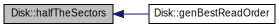
\includegraphics[width=350pt]{classDisk_a7dca6d0d1a9039beca59a0214d8fa32d_icgraph}
\end{center}
\end{figure}


\hypertarget{classDisk_a06365b69899e40c025086108ce433376}{}\index{Disk@{Disk}!num\+Sectors@{num\+Sectors}}
\index{num\+Sectors@{num\+Sectors}!Disk@{Disk}}
\subsubsection[{num\+Sectors}]{\setlength{\rightskip}{0pt plus 5cm}{\bf B\+Y\+T\+E} Disk\+::num\+Sectors (
\begin{DoxyParamCaption}
\item[{{\bf B\+Y\+T\+E}}]{track, }
\item[{{\bf B\+Y\+T\+E}}]{side}
\end{DoxyParamCaption}
)\hspace{0.3cm}{\ttfamily [virtual]}}\label{classDisk_a06365b69899e40c025086108ce433376}
return the number of sectors


\begin{DoxyParams}{Parameters}
{\em track} & \\
\hline
{\em side} & \\
\hline
\end{DoxyParams}
\begin{DoxyReturn}{Returns}
number of sectors 
\end{DoxyReturn}


Definition at line 39 of file disk.\+cpp.

\hypertarget{classDisk_aacfb8782312379d5d6bc65d3c852d864}{}\index{Disk@{Disk}!num\+Sides@{num\+Sides}}
\index{num\+Sides@{num\+Sides}!Disk@{Disk}}
\subsubsection[{num\+Sides}]{\setlength{\rightskip}{0pt plus 5cm}{\bf B\+Y\+T\+E} Disk\+::num\+Sides (
\begin{DoxyParamCaption}
\item[{void}]{}
\end{DoxyParamCaption}
)\hspace{0.3cm}{\ttfamily [virtual]}}\label{classDisk_aacfb8782312379d5d6bc65d3c852d864}
return the number of sides for the disk

\begin{DoxyReturn}{Returns}
number of sides 
\end{DoxyReturn}


Definition at line 16 of file disk.\+cpp.

\hypertarget{classDisk_afeeca1516865154ea3fa3380a784e0c9}{}\index{Disk@{Disk}!num\+Tracks@{num\+Tracks}}
\index{num\+Tracks@{num\+Tracks}!Disk@{Disk}}
\subsubsection[{num\+Tracks}]{\setlength{\rightskip}{0pt plus 5cm}{\bf B\+Y\+T\+E} Disk\+::num\+Tracks (
\begin{DoxyParamCaption}
\item[{void}]{}
\end{DoxyParamCaption}
)\hspace{0.3cm}{\ttfamily [virtual]}}\label{classDisk_afeeca1516865154ea3fa3380a784e0c9}
return the number of tracks for the disk

\begin{DoxyReturn}{Returns}
number of tracks 
\end{DoxyReturn}


Definition at line 26 of file disk.\+cpp.



The documentation for this class was generated from the following files\+:\begin{DoxyCompactItemize}
\item 
\hyperlink{disk_8h}{disk.\+h}\item 
\hyperlink{disk_8cpp}{disk.\+cpp}\end{DoxyCompactItemize}

\hypertarget{classDrive}{}\section{Drive Class Reference}
\label{classDrive}\index{Drive@{Drive}}
\subsection*{Public Member Functions}
\begin{DoxyCompactItemize}
\item 
\hyperlink{classDrive_a4f4e8bf510bd82b4440e89426ee56122}{Drive} (\hyperlink{drive_8h_structDriveInfo}{Drive\+Info} $\ast$drive)
\item 
\hyperlink{classDrive_a9a9f96b1b0b4e841567ccf9fc2d60aaa}{$\sim$\+Drive} ()
\item 
uint8\+\_\+t \hyperlink{classDrive_a7c6f7c9049791e77d26ca6239bc7d274}{get\+Status} ()
\item 
bool \hyperlink{classDrive_a30473c2fd25a65919f11a38be6982c34}{set\+Heads} (uint8\+\_\+t heads)
\item 
bool \hyperlink{classDrive_a102cde6bc5b9af8c7a8e8461c04aa16a}{set\+Tpi} (uint8\+\_\+t tpi)
\item 
bool \hyperlink{classDrive_ac6911a7f8704518bbee6c17b2dad3609}{set\+Rpm} (uint16\+\_\+t rpm)
\item 
\hypertarget{classDrive_a1970efb5b1a6d2d5875541e8e64223a2}{}uint8\+\_\+t {\bfseries get\+Heads} ()\label{classDrive_a1970efb5b1a6d2d5875541e8e64223a2}

\item 
\hypertarget{classDrive_a4c3ab6d75e178f7fbc25dd4253c3487c}{}uint8\+\_\+t {\bfseries get\+Tpi} ()\label{classDrive_a4c3ab6d75e178f7fbc25dd4253c3487c}

\item 
\hypertarget{classDrive_a12704cf292647bdd49d937464ab9b2fd}{}uint16\+\_\+t {\bfseries get\+Rpm} ()\label{classDrive_a12704cf292647bdd49d937464ab9b2fd}

\end{DoxyCompactItemize}
\subsection*{Static Public Member Functions}
\begin{DoxyCompactItemize}
\item 
static \hyperlink{drive_8h_structDriveInfo}{Drive\+Info} $\ast$ \hyperlink{classDrive_a0f266ed4ce8f84a557be46f24c55063c}{get\+\_\+drive\+\_\+list} (void)
\end{DoxyCompactItemize}
\subsection*{Private Attributes}
\begin{DoxyCompactItemize}
\item 
\hypertarget{classDrive_a9e159f1bca0d95a9a045e374650e91c4}{}uint8\+\_\+t {\bfseries status\+\_\+m}\label{classDrive_a9e159f1bca0d95a9a045e374650e91c4}

\item 
\hypertarget{classDrive_afb514e2fca6402ae3c347f05e16a9986}{}uint8\+\_\+t {\bfseries heads\+\_\+m}\label{classDrive_afb514e2fca6402ae3c347f05e16a9986}

\item 
\hypertarget{classDrive_af0f56f9a6d4f541e6692e4eaf5b9a8d5}{}uint8\+\_\+t {\bfseries tpi\+\_\+m}\label{classDrive_af0f56f9a6d4f541e6692e4eaf5b9a8d5}

\item 
\hypertarget{classDrive_a777736f1f50ba6c394808cbb9b8bf051}{}uint16\+\_\+t {\bfseries rpm\+\_\+m}\label{classDrive_a777736f1f50ba6c394808cbb9b8bf051}

\end{DoxyCompactItemize}


\subsection{Detailed Description}


Definition at line 23 of file drive.\+h.



\subsection{Constructor \& Destructor Documentation}
\hypertarget{classDrive_a4f4e8bf510bd82b4440e89426ee56122}{}\index{Drive@{Drive}!Drive@{Drive}}
\index{Drive@{Drive}!Drive@{Drive}}
\subsubsection[{Drive}]{\setlength{\rightskip}{0pt plus 5cm}Drive\+::\+Drive (
\begin{DoxyParamCaption}
\item[{{\bf Drive\+Info} $\ast$}]{drive}
\end{DoxyParamCaption}
)}\label{classDrive_a4f4e8bf510bd82b4440e89426ee56122}
constructor 

Definition at line 18 of file drive.\+cpp.



Here is the call graph for this function\+:\nopagebreak
\begin{figure}[H]
\begin{center}
\leavevmode
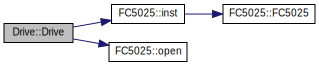
\includegraphics[width=350pt]{classDrive_a4f4e8bf510bd82b4440e89426ee56122_cgraph}
\end{center}
\end{figure}


\hypertarget{classDrive_a9a9f96b1b0b4e841567ccf9fc2d60aaa}{}\index{Drive@{Drive}!````~Drive@{$\sim$\+Drive}}
\index{````~Drive@{$\sim$\+Drive}!Drive@{Drive}}
\subsubsection[{$\sim$\+Drive}]{\setlength{\rightskip}{0pt plus 5cm}Drive\+::$\sim$\+Drive (
\begin{DoxyParamCaption}
{}
\end{DoxyParamCaption}
)}\label{classDrive_a9a9f96b1b0b4e841567ccf9fc2d60aaa}
destructor 

Definition at line 28 of file drive.\+cpp.



Here is the call graph for this function\+:\nopagebreak
\begin{figure}[H]
\begin{center}
\leavevmode
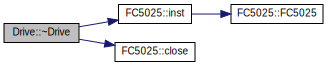
\includegraphics[width=350pt]{classDrive_a9a9f96b1b0b4e841567ccf9fc2d60aaa_cgraph}
\end{center}
\end{figure}




\subsection{Member Function Documentation}
\hypertarget{classDrive_a0f266ed4ce8f84a557be46f24c55063c}{}\index{Drive@{Drive}!get\+\_\+drive\+\_\+list@{get\+\_\+drive\+\_\+list}}
\index{get\+\_\+drive\+\_\+list@{get\+\_\+drive\+\_\+list}!Drive@{Drive}}
\subsubsection[{get\+\_\+drive\+\_\+list}]{\setlength{\rightskip}{0pt plus 5cm}{\bf Drive\+Info} $\ast$ Drive\+::get\+\_\+drive\+\_\+list (
\begin{DoxyParamCaption}
\item[{void}]{}
\end{DoxyParamCaption}
)\hspace{0.3cm}{\ttfamily [static]}}\label{classDrive_a0f266ed4ce8f84a557be46f24c55063c}
get drive list

\begin{DoxyReturn}{Returns}
drive info 
\end{DoxyReturn}


Definition at line 86 of file drive.\+cpp.



Here is the call graph for this function\+:\nopagebreak
\begin{figure}[H]
\begin{center}
\leavevmode
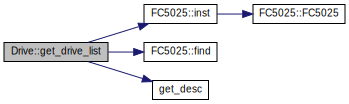
\includegraphics[width=350pt]{classDrive_a0f266ed4ce8f84a557be46f24c55063c_cgraph}
\end{center}
\end{figure}


\hypertarget{classDrive_a7c6f7c9049791e77d26ca6239bc7d274}{}\index{Drive@{Drive}!get\+Status@{get\+Status}}
\index{get\+Status@{get\+Status}!Drive@{Drive}}
\subsubsection[{get\+Status}]{\setlength{\rightskip}{0pt plus 5cm}uint8\+\_\+t Drive\+::get\+Status (
\begin{DoxyParamCaption}
{}
\end{DoxyParamCaption}
)}\label{classDrive_a7c6f7c9049791e77d26ca6239bc7d274}
get status

\begin{DoxyReturn}{Returns}
staus 
\end{DoxyReturn}


Definition at line 39 of file drive.\+cpp.

\hypertarget{classDrive_a30473c2fd25a65919f11a38be6982c34}{}\index{Drive@{Drive}!set\+Heads@{set\+Heads}}
\index{set\+Heads@{set\+Heads}!Drive@{Drive}}
\subsubsection[{set\+Heads}]{\setlength{\rightskip}{0pt plus 5cm}bool Drive\+::set\+Heads (
\begin{DoxyParamCaption}
\item[{uint8\+\_\+t}]{heads}
\end{DoxyParamCaption}
)}\label{classDrive_a30473c2fd25a65919f11a38be6982c34}
set number of heads for the drive


\begin{DoxyParams}{Parameters}
{\em heads} & \\
\hline
\end{DoxyParams}
\begin{DoxyReturn}{Returns}
success 
\end{DoxyReturn}


Definition at line 163 of file drive.\+cpp.

\hypertarget{classDrive_ac6911a7f8704518bbee6c17b2dad3609}{}\index{Drive@{Drive}!set\+Rpm@{set\+Rpm}}
\index{set\+Rpm@{set\+Rpm}!Drive@{Drive}}
\subsubsection[{set\+Rpm}]{\setlength{\rightskip}{0pt plus 5cm}bool Drive\+::set\+Rpm (
\begin{DoxyParamCaption}
\item[{uint16\+\_\+t}]{rpm}
\end{DoxyParamCaption}
)}\label{classDrive_ac6911a7f8704518bbee6c17b2dad3609}
set R\+P\+M of the drive


\begin{DoxyParams}{Parameters}
{\em rpm} & return success \\
\hline
\end{DoxyParams}


Definition at line 205 of file drive.\+cpp.

\hypertarget{classDrive_a102cde6bc5b9af8c7a8e8461c04aa16a}{}\index{Drive@{Drive}!set\+Tpi@{set\+Tpi}}
\index{set\+Tpi@{set\+Tpi}!Drive@{Drive}}
\subsubsection[{set\+Tpi}]{\setlength{\rightskip}{0pt plus 5cm}bool Drive\+::set\+Tpi (
\begin{DoxyParamCaption}
\item[{uint8\+\_\+t}]{tpi}
\end{DoxyParamCaption}
)}\label{classDrive_a102cde6bc5b9af8c7a8e8461c04aa16a}
set tpi for the drive


\begin{DoxyParams}{Parameters}
{\em tpi} & \\
\hline
\end{DoxyParams}
\begin{DoxyReturn}{Returns}
success 
\end{DoxyReturn}


Definition at line 184 of file drive.\+cpp.



The documentation for this class was generated from the following files\+:\begin{DoxyCompactItemize}
\item 
\hyperlink{drive_8h}{drive.\+h}\item 
\hyperlink{drive_8cpp}{drive.\+cpp}\end{DoxyCompactItemize}

\hypertarget{classFC5025}{}\section{F\+C5025 Class Reference}
\label{classFC5025}\index{F\+C5025@{F\+C5025}}


Collaboration diagram for F\+C5025\+:\nopagebreak
\begin{figure}[H]
\begin{center}
\leavevmode
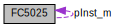
\includegraphics[width=188pt]{classFC5025__coll__graph}
\end{center}
\end{figure}
\subsection*{Public Types}
\begin{DoxyCompactItemize}
\item 
\hypertarget{classFC5025_a20c6ea9759857c2a4035ee76812ab68f}{}enum {\bfseries Opcode} \+: uint8\+\_\+t \{ \\*
{\bfseries Seek} = 0xc0, 
{\bfseries Self\+Test} = 0xc1, 
{\bfseries Flags} = 0xc2, 
{\bfseries Drive\+Status} = 0xc3, 
\\*
{\bfseries Indexes} = 0xc4, 
{\bfseries Read\+Flexible} = 0xc6, 
{\bfseries Read\+Id} = 0xc7
 \}\label{classFC5025_a20c6ea9759857c2a4035ee76812ab68f}

\item 
\hypertarget{classFC5025_a5c77c7b92ba3ef9204ce67d76dc62f8c}{}enum {\bfseries Format} \+: uint8\+\_\+t \{ {\bfseries Apple\+G\+C\+R} = 1, 
{\bfseries Commodore\+G\+C\+R} = 2, 
{\bfseries F\+M} = 3, 
{\bfseries M\+F\+M} = 4
 \}\label{classFC5025_a5c77c7b92ba3ef9204ce67d76dc62f8c}

\item 
\hypertarget{classFC5025_af1902ae236f23ab73eb0d64f737b3095}{}enum {\bfseries Density} \+: uint8\+\_\+t \label{classFC5025_af1902ae236f23ab73eb0d64f737b3095}

\item 
\hypertarget{classFC5025_af510c7f00e18b356f791b31be8101a2e}{}enum {\bfseries Key} \+: uint8\+\_\+t \{ {\bfseries No\+Error} = 0, 
{\bfseries Seek\+Error} = 2, 
{\bfseries Diag\+Error} = 4, 
{\bfseries Command\+Error} = 5
 \}\label{classFC5025_af510c7f00e18b356f791b31be8101a2e}

\item 
\hypertarget{classFC5025_aca67e0584955f19ae89c3be0fa2ed562}{}enum {\bfseries A\+S\+C\+\_\+\+Seek} \+: uint8\+\_\+t \{ {\bfseries No\+Reference\+Position} = 6
 \}\label{classFC5025_aca67e0584955f19ae89c3be0fa2ed562}

\item 
\hypertarget{classFC5025_ada53660e7071c46026f58d5bb85fe5d5}{}enum {\bfseries A\+S\+C\+\_\+\+Diag} \+: uint8\+\_\+t \{ {\bfseries Diagnotic\+Failure} = 0x40
 \}\label{classFC5025_ada53660e7071c46026f58d5bb85fe5d5}

\item 
\hypertarget{classFC5025_a2552265feefbe42c9bb4bc8064c440c3}{}enum {\bfseries A\+S\+C\+Q\+\_\+\+Diag} \+: uint8\+\_\+t \{ {\bfseries Diagnotic\+Failure} = 0x80
 \}\label{classFC5025_a2552265feefbe42c9bb4bc8064c440c3}

\item 
\hypertarget{classFC5025_a96c5fbc52b7a2a52e83eb379a1fd28a2}{}enum {\bfseries A\+S\+C\+\_\+\+Command} \+: uint8\+\_\+t \{ {\bfseries Invalid\+Command} = 0x20, 
{\bfseries Invalid\+Field} = 0x24, 
{\bfseries Sequence\+Error} = 0x2c
 \}\label{classFC5025_a96c5fbc52b7a2a52e83eb379a1fd28a2}

\end{DoxyCompactItemize}
\subsection*{Public Member Functions}
\begin{DoxyCompactItemize}
\item 
int \hyperlink{classFC5025_ac645d8e876d7121ca75db81ef99ee7f4}{bulk\+C\+D\+B} (void $\ast$cdb, int length, int timeout, uint8\+\_\+t $\ast$csw\+\_\+out, uint8\+\_\+t $\ast$xferbuf, int xferlen, int $\ast$xferlen\+\_\+out)
\item 
int \hyperlink{classFC5025_a867a0dfff92f111697ca74655bb42d26}{recalibrate} (void)
\item 
int \hyperlink{classFC5025_ab38385df803acdde0c55e472669ffc2d}{seek} (uint8\+\_\+t track)
\item 
int \hyperlink{classFC5025_aa796eca9259c5c1718e09184d94630a9}{read\+Id} (uint8\+\_\+t $\ast$out, int length, uint8\+\_\+t side, uint8\+\_\+t format, int bitcell, uint8\+\_\+t idam0, uint8\+\_\+t idam1, uint8\+\_\+t idam2)
\item 
int \hyperlink{classFC5025_a9c372002cbdc43034ed601f022e22751}{flags} (uint8\+\_\+t in, uint8\+\_\+t mask, int $\ast$out)
\item 
int \hyperlink{classFC5025_afff5293f6d1011a7b107607f544fedf5}{set\+Density} (int density)
\item 
int \hyperlink{classFC5025_a59d919ef113972193186371c7db7ee9d}{open} (struct usb\+\_\+device $\ast$dev)
\item 
int \hyperlink{classFC5025_a52c3aa7a28679f4afb203805f4c33510}{close} (void)
\item 
int \hyperlink{classFC5025_a644103f08f11ac57a1faf8710a3d7b4c}{find} (struct usb\+\_\+device $\ast$$\ast$devs, int max)
\item 
int \hyperlink{classFC5025_a178ad6a12a928f270db02fdbb463db95}{drive\+Status} (uint8\+\_\+t $\ast$track, uint16\+\_\+t $\ast$speed, uint8\+\_\+t $\ast$sector\+Count, uint8\+\_\+t $\ast$\hyperlink{classFC5025_a9c372002cbdc43034ed601f022e22751}{flags})
\item 
void \hyperlink{classFC5025_a794efc97b600cfa4e5c942458cdf3833}{configure\+Disk\+Drive} (uint8\+\_\+t tracks, uint8\+\_\+t sides, uint16\+\_\+t rpm, uint8\+\_\+t step\+Rate)
\item 
void \hyperlink{classFC5025_a2277f14f5c11732eeabff350d1aa3203}{get\+Disk\+Drive} (uint8\+\_\+t \&tracks, uint8\+\_\+t \&sides, uint16\+\_\+t \&rpm, uint8\+\_\+t \&step\+Rate)
\item 
void \hyperlink{classFC5025_af4a65dba5d2145adc0a0bb69d8ce6ae0}{configure\+Floppy\+Disk} (uint8\+\_\+t tracks, uint8\+\_\+t sides, uint16\+\_\+t rpm)
\end{DoxyCompactItemize}
\subsection*{Static Public Member Functions}
\begin{DoxyCompactItemize}
\item 
static \hyperlink{classFC5025}{F\+C5025} $\ast$ \hyperlink{classFC5025_a3fa1262c4bde8788a2d71d07dfc88630}{inst} ()
\end{DoxyCompactItemize}
\subsection*{Static Public Attributes}
\begin{DoxyCompactItemize}
\item 
\hypertarget{classFC5025_a81fe505f0571c2840b5ac3a0e055d510}{}static const uint8\+\_\+t {\bfseries Read\+Flag\+\_\+\+Side\+\_\+c} = 0x01\label{classFC5025_a81fe505f0571c2840b5ac3a0e055d510}

\item 
\hypertarget{classFC5025_a41fd525aaaa28348be523122c2dd5c63}{}static const uint8\+\_\+t {\bfseries Read\+Flag\+\_\+\+Id\+Field\+\_\+c} = 0x02\label{classFC5025_a41fd525aaaa28348be523122c2dd5c63}

\item 
\hypertarget{classFC5025_a40dc0e101b49a93d22ab60398dc55ca1}{}static const uint8\+\_\+t {\bfseries Read\+Flag\+\_\+\+Overrun\+Recovery\+\_\+c} = 0x04\label{classFC5025_a40dc0e101b49a93d22ab60398dc55ca1}

\item 
\hypertarget{classFC5025_a1a862121d6b98c13b3cc4249cee333ea}{}static const uint8\+\_\+t {\bfseries Read\+Flag\+\_\+\+No\+Autosync\+\_\+c} = 0x08\label{classFC5025_a1a862121d6b98c13b3cc4249cee333ea}

\item 
\hypertarget{classFC5025_aaf2e391a9013cb2fc59dc7ca2559a437}{}static const uint8\+\_\+t {\bfseries Read\+Flag\+\_\+\+Angular\+\_\+c} = 0x10\label{classFC5025_aaf2e391a9013cb2fc59dc7ca2559a437}

\item 
\hypertarget{classFC5025_ac3fdb86284d3dc63ef845b4c4dc66ec6}{}static const uint8\+\_\+t {\bfseries Read\+Flag\+\_\+\+No\+Adaptive\+\_\+c} = 0x20\label{classFC5025_ac3fdb86284d3dc63ef845b4c4dc66ec6}

\end{DoxyCompactItemize}
\subsection*{Private Member Functions}
\begin{DoxyCompactItemize}
\item 
\hyperlink{classFC5025_a01786b9fd3a20919da5e702794fa95e6}{F\+C5025} ()
\item 
virtual \hyperlink{classFC5025_a5ceae55a353876d38857b965e87e6aeb}{$\sim$\+F\+C5025} ()
\item 
int \hyperlink{classFC5025_ad03589bd35682da51fe0cb2e7523688d}{internal\+Seek} (uint8\+\_\+t mode, uint8\+\_\+t step\+Rate, uint8\+\_\+t track)
\end{DoxyCompactItemize}
\subsection*{Private Attributes}
\begin{DoxyCompactItemize}
\item 
\hypertarget{classFC5025_abf6e25d1e52203481358c5cfe3e7af37}{}usb\+\_\+dev\+\_\+handle $\ast$ {\bfseries udev\+\_\+m}\label{classFC5025_abf6e25d1e52203481358c5cfe3e7af37}

\item 
\hypertarget{classFC5025_ad8e41355041f79941a2ae31a2398c20a}{}uint8\+\_\+t {\bfseries last\+Sense\+Key\+\_\+m}\label{classFC5025_ad8e41355041f79941a2ae31a2398c20a}

\item 
\hypertarget{classFC5025_aded61ba4384be70cf0519be5e79da8bb}{}uint8\+\_\+t {\bfseries last\+A\+S\+C\+\_\+m}\label{classFC5025_aded61ba4384be70cf0519be5e79da8bb}

\item 
\hypertarget{classFC5025_a4fd804183b18b85ae5da66dd9d2f288f}{}uint8\+\_\+t {\bfseries last\+A\+S\+C\+Q\+\_\+m}\label{classFC5025_a4fd804183b18b85ae5da66dd9d2f288f}

\item 
\hypertarget{classFC5025_a7d38def4944d0fc41a700f5acb89827a}{}uint8\+\_\+t {\bfseries drive\+\_\+\+Tracks\+\_\+m}\label{classFC5025_a7d38def4944d0fc41a700f5acb89827a}

\item 
\hypertarget{classFC5025_a059f7ea221799ed790c7a72c7ac4606e}{}uint8\+\_\+t {\bfseries drive\+\_\+\+Sides\+\_\+m}\label{classFC5025_a059f7ea221799ed790c7a72c7ac4606e}

\item 
\hypertarget{classFC5025_ad3b4907b0ef1e13b33b60b65c07bbb00}{}uint16\+\_\+t {\bfseries drive\+\_\+\+R\+P\+M\+\_\+m}\label{classFC5025_ad3b4907b0ef1e13b33b60b65c07bbb00}

\item 
\hypertarget{classFC5025_aaea018a0fb54263219f7a5991889dec0}{}uint8\+\_\+t {\bfseries drive\+\_\+\+Step\+Rate\+\_\+m}\label{classFC5025_aaea018a0fb54263219f7a5991889dec0}

\item 
\hypertarget{classFC5025_a7857b1f818b0a9489bb0476a0621529d}{}uint8\+\_\+t {\bfseries disk\+\_\+\+Tracks\+\_\+m}\label{classFC5025_a7857b1f818b0a9489bb0476a0621529d}

\item 
\hypertarget{classFC5025_aa643620f521f2ee83b70a79ad81704b2}{}uint8\+\_\+t {\bfseries disk\+\_\+\+Sides\+\_\+m}\label{classFC5025_aa643620f521f2ee83b70a79ad81704b2}

\item 
\hypertarget{classFC5025_a6b142a76cdcf4ab3b901c82290a534b4}{}uint16\+\_\+t {\bfseries disk\+\_\+\+R\+P\+M\+\_\+m}\label{classFC5025_a6b142a76cdcf4ab3b901c82290a534b4}

\end{DoxyCompactItemize}
\subsection*{Static Private Attributes}
\begin{DoxyCompactItemize}
\item 
\hypertarget{classFC5025_ab2baec0c4357e5e9a1dcbb5ab2826dac}{}static \hyperlink{classFC5025}{F\+C5025} $\ast$ {\bfseries p\+Inst\+\_\+m} = nullptr\label{classFC5025_ab2baec0c4357e5e9a1dcbb5ab2826dac}

\item 
\hypertarget{classFC5025_ae52af5b012e31fac220c555b8e75c16b}{}static const uint16\+\_\+t {\bfseries Vendor\+I\+D\+\_\+c} = 0x16c0\label{classFC5025_ae52af5b012e31fac220c555b8e75c16b}

\item 
\hypertarget{classFC5025_a6fbbb73e88aa88a86093030aa8ff2165}{}static const uint16\+\_\+t {\bfseries Product\+I\+D\+\_\+c} = 0x06d6\label{classFC5025_a6fbbb73e88aa88a86093030aa8ff2165}

\item 
\hypertarget{classFC5025_a9b59e60426e62388838366955ad7cdaf}{}static const uint32\+\_\+t {\bfseries csw\+Signature\+\_\+c} = 0x46435342\label{classFC5025_a9b59e60426e62388838366955ad7cdaf}

\end{DoxyCompactItemize}


\subsection{Detailed Description}


Definition at line 25 of file fc5025.\+h.



\subsection{Constructor \& Destructor Documentation}
\hypertarget{classFC5025_a01786b9fd3a20919da5e702794fa95e6}{}\index{F\+C5025@{F\+C5025}!F\+C5025@{F\+C5025}}
\index{F\+C5025@{F\+C5025}!F\+C5025@{F\+C5025}}
\subsubsection[{F\+C5025}]{\setlength{\rightskip}{0pt plus 5cm}F\+C5025\+::\+F\+C5025 (
\begin{DoxyParamCaption}
{}
\end{DoxyParamCaption}
)\hspace{0.3cm}{\ttfamily [private]}}\label{classFC5025_a01786b9fd3a20919da5e702794fa95e6}
Constructor 

Definition at line 49 of file fc5025.\+cpp.



Here is the caller graph for this function\+:\nopagebreak
\begin{figure}[H]
\begin{center}
\leavevmode
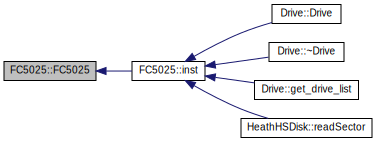
\includegraphics[width=350pt]{classFC5025_a01786b9fd3a20919da5e702794fa95e6_icgraph}
\end{center}
\end{figure}


\hypertarget{classFC5025_a5ceae55a353876d38857b965e87e6aeb}{}\index{F\+C5025@{F\+C5025}!````~F\+C5025@{$\sim$\+F\+C5025}}
\index{````~F\+C5025@{$\sim$\+F\+C5025}!F\+C5025@{F\+C5025}}
\subsubsection[{$\sim$\+F\+C5025}]{\setlength{\rightskip}{0pt plus 5cm}F\+C5025\+::$\sim$\+F\+C5025 (
\begin{DoxyParamCaption}
{}
\end{DoxyParamCaption}
)\hspace{0.3cm}{\ttfamily [private]}, {\ttfamily [virtual]}}\label{classFC5025_a5ceae55a353876d38857b965e87e6aeb}
Destructor 

Definition at line 79 of file fc5025.\+cpp.



\subsection{Member Function Documentation}
\hypertarget{classFC5025_ac645d8e876d7121ca75db81ef99ee7f4}{}\index{F\+C5025@{F\+C5025}!bulk\+C\+D\+B@{bulk\+C\+D\+B}}
\index{bulk\+C\+D\+B@{bulk\+C\+D\+B}!F\+C5025@{F\+C5025}}
\subsubsection[{bulk\+C\+D\+B}]{\setlength{\rightskip}{0pt plus 5cm}int F\+C5025\+::bulk\+C\+D\+B (
\begin{DoxyParamCaption}
\item[{void $\ast$}]{cdb, }
\item[{int}]{length, }
\item[{int}]{timeout, }
\item[{uint8\+\_\+t $\ast$}]{csw\+\_\+out, }
\item[{uint8\+\_\+t $\ast$}]{xferbuf, }
\item[{int}]{xferlen, }
\item[{int $\ast$}]{xferlen\+\_\+out}
\end{DoxyParamCaption}
)}\label{classFC5025_ac645d8e876d7121ca75db81ef99ee7f4}
common cdb


\begin{DoxyParams}{Parameters}
{\em cdb} & \\
\hline
{\em length} & \\
\hline
{\em timeout} & \\
\hline
{\em csw\+\_\+out} & \\
\hline
{\em xferbuf} & \\
\hline
{\em xferlen} & \\
\hline
{\em xferlen\+\_\+out} & \\
\hline
\end{DoxyParams}
\begin{DoxyReturn}{Returns}
status 
\end{DoxyReturn}


Definition at line 115 of file fc5025.\+cpp.



Here is the caller graph for this function\+:\nopagebreak
\begin{figure}[H]
\begin{center}
\leavevmode
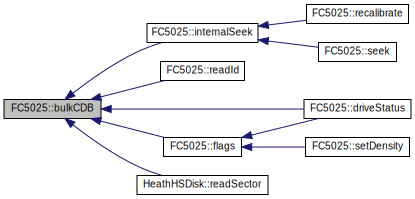
\includegraphics[width=350pt]{classFC5025_ac645d8e876d7121ca75db81ef99ee7f4_icgraph}
\end{center}
\end{figure}


\hypertarget{classFC5025_a52c3aa7a28679f4afb203805f4c33510}{}\index{F\+C5025@{F\+C5025}!close@{close}}
\index{close@{close}!F\+C5025@{F\+C5025}}
\subsubsection[{close}]{\setlength{\rightskip}{0pt plus 5cm}int F\+C5025\+::close (
\begin{DoxyParamCaption}
\item[{void}]{}
\end{DoxyParamCaption}
)}\label{classFC5025_a52c3aa7a28679f4afb203805f4c33510}
close device

\begin{DoxyReturn}{Returns}
status 
\end{DoxyReturn}


Definition at line 468 of file fc5025.\+cpp.



Here is the caller graph for this function\+:\nopagebreak
\begin{figure}[H]
\begin{center}
\leavevmode
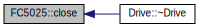
\includegraphics[width=271pt]{classFC5025_a52c3aa7a28679f4afb203805f4c33510_icgraph}
\end{center}
\end{figure}


\hypertarget{classFC5025_a794efc97b600cfa4e5c942458cdf3833}{}\index{F\+C5025@{F\+C5025}!configure\+Disk\+Drive@{configure\+Disk\+Drive}}
\index{configure\+Disk\+Drive@{configure\+Disk\+Drive}!F\+C5025@{F\+C5025}}
\subsubsection[{configure\+Disk\+Drive}]{\setlength{\rightskip}{0pt plus 5cm}void F\+C5025\+::configure\+Disk\+Drive (
\begin{DoxyParamCaption}
\item[{uint8\+\_\+t}]{tracks, }
\item[{uint8\+\_\+t}]{sides, }
\item[{uint16\+\_\+t}]{rpm, }
\item[{uint8\+\_\+t}]{step\+Rate}
\end{DoxyParamCaption}
)}\label{classFC5025_a794efc97b600cfa4e5c942458cdf3833}
configure disk drive


\begin{DoxyParams}{Parameters}
{\em tracks} & \\
\hline
{\em sides} & \\
\hline
{\em rpm} & \\
\hline
{\em step\+Rate} & \\
\hline
\end{DoxyParams}
\begin{DoxyReturn}{Returns}
void 
\end{DoxyReturn}


Definition at line 527 of file fc5025.\+cpp.

\hypertarget{classFC5025_af4a65dba5d2145adc0a0bb69d8ce6ae0}{}\index{F\+C5025@{F\+C5025}!configure\+Floppy\+Disk@{configure\+Floppy\+Disk}}
\index{configure\+Floppy\+Disk@{configure\+Floppy\+Disk}!F\+C5025@{F\+C5025}}
\subsubsection[{configure\+Floppy\+Disk}]{\setlength{\rightskip}{0pt plus 5cm}void F\+C5025\+::configure\+Floppy\+Disk (
\begin{DoxyParamCaption}
\item[{uint8\+\_\+t}]{tracks, }
\item[{uint8\+\_\+t}]{sides, }
\item[{uint16\+\_\+t}]{rpm}
\end{DoxyParamCaption}
)}\label{classFC5025_af4a65dba5d2145adc0a0bb69d8ce6ae0}
configure floppy disk


\begin{DoxyParams}{Parameters}
{\em tracks} & \\
\hline
{\em sides} & \\
\hline
{\em rpm} & \\
\hline
\end{DoxyParams}
\begin{DoxyReturn}{Returns}
void 
\end{DoxyReturn}


Definition at line 570 of file fc5025.\+cpp.

\hypertarget{classFC5025_a178ad6a12a928f270db02fdbb463db95}{}\index{F\+C5025@{F\+C5025}!drive\+Status@{drive\+Status}}
\index{drive\+Status@{drive\+Status}!F\+C5025@{F\+C5025}}
\subsubsection[{drive\+Status}]{\setlength{\rightskip}{0pt plus 5cm}int F\+C5025\+::drive\+Status (
\begin{DoxyParamCaption}
\item[{uint8\+\_\+t $\ast$}]{track, }
\item[{uint16\+\_\+t $\ast$}]{disk\+Speed, }
\item[{uint8\+\_\+t $\ast$}]{sector\+Count, }
\item[{uint8\+\_\+t $\ast$}]{ds\+\_\+flags}
\end{DoxyParamCaption}
)}\label{classFC5025_a178ad6a12a928f270db02fdbb463db95}
get drive status


\begin{DoxyParams}{Parameters}
{\em track} & \\
\hline
{\em disk\+Speed} & \\
\hline
{\em sector\+Count} & \\
\hline
{\em ds\+\_\+flags} & \\
\hline
\end{DoxyParams}
\begin{DoxyReturn}{Returns}
status 
\end{DoxyReturn}


Definition at line 382 of file fc5025.\+cpp.



Here is the call graph for this function\+:\nopagebreak
\begin{figure}[H]
\begin{center}
\leavevmode
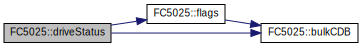
\includegraphics[width=350pt]{classFC5025_a178ad6a12a928f270db02fdbb463db95_cgraph}
\end{center}
\end{figure}


\hypertarget{classFC5025_a644103f08f11ac57a1faf8710a3d7b4c}{}\index{F\+C5025@{F\+C5025}!find@{find}}
\index{find@{find}!F\+C5025@{F\+C5025}}
\subsubsection[{find}]{\setlength{\rightskip}{0pt plus 5cm}int F\+C5025\+::find (
\begin{DoxyParamCaption}
\item[{struct usb\+\_\+device $\ast$$\ast$}]{devs, }
\item[{int}]{max}
\end{DoxyParamCaption}
)}\label{classFC5025_a644103f08f11ac57a1faf8710a3d7b4c}
find devices


\begin{DoxyParams}{Parameters}
{\em devs} & list of the devices found \\
\hline
{\em max} & maximum number of devices to return\\
\hline
\end{DoxyParams}
\begin{DoxyReturn}{Returns}
number of devices found 
\end{DoxyReturn}


Definition at line 487 of file fc5025.\+cpp.



Here is the caller graph for this function\+:\nopagebreak
\begin{figure}[H]
\begin{center}
\leavevmode
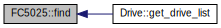
\includegraphics[width=293pt]{classFC5025_a644103f08f11ac57a1faf8710a3d7b4c_icgraph}
\end{center}
\end{figure}


\hypertarget{classFC5025_a9c372002cbdc43034ed601f022e22751}{}\index{F\+C5025@{F\+C5025}!flags@{flags}}
\index{flags@{flags}!F\+C5025@{F\+C5025}}
\subsubsection[{flags}]{\setlength{\rightskip}{0pt plus 5cm}int F\+C5025\+::flags (
\begin{DoxyParamCaption}
\item[{uint8\+\_\+t}]{in, }
\item[{uint8\+\_\+t}]{mask, }
\item[{int $\ast$}]{out}
\end{DoxyParamCaption}
)}\label{classFC5025_a9c372002cbdc43034ed601f022e22751}
set flags


\begin{DoxyParams}{Parameters}
{\em in} & \\
\hline
{\em mask} & \\
\hline
{\em out} & \\
\hline
\end{DoxyParams}
\begin{DoxyReturn}{Returns}
status 
\end{DoxyReturn}


Definition at line 338 of file fc5025.\+cpp.



Here is the call graph for this function\+:\nopagebreak
\begin{figure}[H]
\begin{center}
\leavevmode
\includegraphics[width=291pt]{classFC5025_a9c372002cbdc43034ed601f022e22751_cgraph}
\end{center}
\end{figure}




Here is the caller graph for this function\+:\nopagebreak
\begin{figure}[H]
\begin{center}
\leavevmode
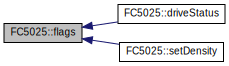
\includegraphics[width=301pt]{classFC5025_a9c372002cbdc43034ed601f022e22751_icgraph}
\end{center}
\end{figure}


\hypertarget{classFC5025_a2277f14f5c11732eeabff350d1aa3203}{}\index{F\+C5025@{F\+C5025}!get\+Disk\+Drive@{get\+Disk\+Drive}}
\index{get\+Disk\+Drive@{get\+Disk\+Drive}!F\+C5025@{F\+C5025}}
\subsubsection[{get\+Disk\+Drive}]{\setlength{\rightskip}{0pt plus 5cm}void F\+C5025\+::get\+Disk\+Drive (
\begin{DoxyParamCaption}
\item[{uint8\+\_\+t \&}]{tracks, }
\item[{uint8\+\_\+t \&}]{sides, }
\item[{uint16\+\_\+t \&}]{rpm, }
\item[{uint8\+\_\+t \&}]{step\+Rate}
\end{DoxyParamCaption}
)}\label{classFC5025_a2277f14f5c11732eeabff350d1aa3203}
get disk drive


\begin{DoxyParams}{Parameters}
{\em tracks} & \\
\hline
{\em sides} & \\
\hline
{\em rpm} & \\
\hline
{\em step\+Rate} & \\
\hline
\end{DoxyParams}
\begin{DoxyReturn}{Returns}
void 
\end{DoxyReturn}


Definition at line 549 of file fc5025.\+cpp.

\hypertarget{classFC5025_a3fa1262c4bde8788a2d71d07dfc88630}{}\index{F\+C5025@{F\+C5025}!inst@{inst}}
\index{inst@{inst}!F\+C5025@{F\+C5025}}
\subsubsection[{inst}]{\setlength{\rightskip}{0pt plus 5cm}{\bf F\+C5025} $\ast$ F\+C5025\+::inst (
\begin{DoxyParamCaption}
{}
\end{DoxyParamCaption}
)\hspace{0.3cm}{\ttfamily [static]}}\label{classFC5025_a3fa1262c4bde8788a2d71d07dfc88630}
get singleton

\begin{DoxyReturn}{Returns}
\hyperlink{classFC5025}{F\+C5025} 
\end{DoxyReturn}


Definition at line 90 of file fc5025.\+cpp.



Here is the call graph for this function\+:\nopagebreak
\begin{figure}[H]
\begin{center}
\leavevmode
\includegraphics[width=281pt]{classFC5025_a3fa1262c4bde8788a2d71d07dfc88630_cgraph}
\end{center}
\end{figure}




Here is the caller graph for this function\+:\nopagebreak
\begin{figure}[H]
\begin{center}
\leavevmode
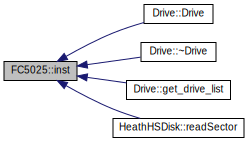
\includegraphics[width=320pt]{classFC5025_a3fa1262c4bde8788a2d71d07dfc88630_icgraph}
\end{center}
\end{figure}


\hypertarget{classFC5025_ad03589bd35682da51fe0cb2e7523688d}{}\index{F\+C5025@{F\+C5025}!internal\+Seek@{internal\+Seek}}
\index{internal\+Seek@{internal\+Seek}!F\+C5025@{F\+C5025}}
\subsubsection[{internal\+Seek}]{\setlength{\rightskip}{0pt plus 5cm}int F\+C5025\+::internal\+Seek (
\begin{DoxyParamCaption}
\item[{uint8\+\_\+t}]{mode, }
\item[{uint8\+\_\+t}]{step\+Rate, }
\item[{uint8\+\_\+t}]{track}
\end{DoxyParamCaption}
)\hspace{0.3cm}{\ttfamily [private]}}\label{classFC5025_ad03589bd35682da51fe0cb2e7523688d}
internal seek command


\begin{DoxyParams}{Parameters}
{\em mode} & \\
\hline
{\em step\+Rate} & \\
\hline
{\em track} & \\
\hline
\end{DoxyParams}
\begin{DoxyReturn}{Returns}
status 
\end{DoxyReturn}


Definition at line 222 of file fc5025.\+cpp.



Here is the call graph for this function\+:\nopagebreak
\begin{figure}[H]
\begin{center}
\leavevmode
\includegraphics[width=324pt]{classFC5025_ad03589bd35682da51fe0cb2e7523688d_cgraph}
\end{center}
\end{figure}




Here is the caller graph for this function\+:\nopagebreak
\begin{figure}[H]
\begin{center}
\leavevmode
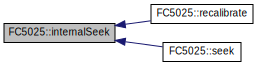
\includegraphics[width=329pt]{classFC5025_ad03589bd35682da51fe0cb2e7523688d_icgraph}
\end{center}
\end{figure}


\hypertarget{classFC5025_a59d919ef113972193186371c7db7ee9d}{}\index{F\+C5025@{F\+C5025}!open@{open}}
\index{open@{open}!F\+C5025@{F\+C5025}}
\subsubsection[{open}]{\setlength{\rightskip}{0pt plus 5cm}int F\+C5025\+::open (
\begin{DoxyParamCaption}
\item[{struct usb\+\_\+device $\ast$}]{dev}
\end{DoxyParamCaption}
)}\label{classFC5025_a59d919ef113972193186371c7db7ee9d}
open device


\begin{DoxyParams}{Parameters}
{\em dev} & device to open\\
\hline
\end{DoxyParams}
\begin{DoxyReturn}{Returns}
0 -\/ success, 1 -\/ failure 
\end{DoxyReturn}


Definition at line 443 of file fc5025.\+cpp.



Here is the caller graph for this function\+:\nopagebreak
\begin{figure}[H]
\begin{center}
\leavevmode
\includegraphics[width=263pt]{classFC5025_a59d919ef113972193186371c7db7ee9d_icgraph}
\end{center}
\end{figure}


\hypertarget{classFC5025_aa796eca9259c5c1718e09184d94630a9}{}\index{F\+C5025@{F\+C5025}!read\+Id@{read\+Id}}
\index{read\+Id@{read\+Id}!F\+C5025@{F\+C5025}}
\subsubsection[{read\+Id}]{\setlength{\rightskip}{0pt plus 5cm}int F\+C5025\+::read\+Id (
\begin{DoxyParamCaption}
\item[{uint8\+\_\+t $\ast$}]{out, }
\item[{int}]{length, }
\item[{uint8\+\_\+t}]{side, }
\item[{uint8\+\_\+t}]{format, }
\item[{int}]{bitcell, }
\item[{uint8\+\_\+t}]{idam0, }
\item[{uint8\+\_\+t}]{idam1, }
\item[{uint8\+\_\+t}]{idam2}
\end{DoxyParamCaption}
)}\label{classFC5025_aa796eca9259c5c1718e09184d94630a9}
read id


\begin{DoxyParams}{Parameters}
{\em out} & \\
\hline
{\em length} & \\
\hline
{\em side} & \\
\hline
{\em format} & \\
\hline
{\em bitcell} & \\
\hline
{\em idam0} & \\
\hline
{\em idam1} & \\
\hline
{\em idam2} & \\
\hline
\end{DoxyParams}
\begin{DoxyReturn}{Returns}
status 
\end{DoxyReturn}


Definition at line 287 of file fc5025.\+cpp.



Here is the call graph for this function\+:\nopagebreak
\begin{figure}[H]
\begin{center}
\leavevmode
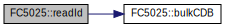
\includegraphics[width=297pt]{classFC5025_aa796eca9259c5c1718e09184d94630a9_cgraph}
\end{center}
\end{figure}


\hypertarget{classFC5025_a867a0dfff92f111697ca74655bb42d26}{}\index{F\+C5025@{F\+C5025}!recalibrate@{recalibrate}}
\index{recalibrate@{recalibrate}!F\+C5025@{F\+C5025}}
\subsubsection[{recalibrate}]{\setlength{\rightskip}{0pt plus 5cm}int F\+C5025\+::recalibrate (
\begin{DoxyParamCaption}
\item[{void}]{}
\end{DoxyParamCaption}
)}\label{classFC5025_a867a0dfff92f111697ca74655bb42d26}
recalibrate -\/ try to find track zero

\begin{DoxyReturn}{Returns}
status 
\end{DoxyReturn}


Definition at line 254 of file fc5025.\+cpp.



Here is the call graph for this function\+:\nopagebreak
\begin{figure}[H]
\begin{center}
\leavevmode
\includegraphics[width=350pt]{classFC5025_a867a0dfff92f111697ca74655bb42d26_cgraph}
\end{center}
\end{figure}


\hypertarget{classFC5025_ab38385df803acdde0c55e472669ffc2d}{}\index{F\+C5025@{F\+C5025}!seek@{seek}}
\index{seek@{seek}!F\+C5025@{F\+C5025}}
\subsubsection[{seek}]{\setlength{\rightskip}{0pt plus 5cm}int F\+C5025\+::seek (
\begin{DoxyParamCaption}
\item[{uint8\+\_\+t}]{track}
\end{DoxyParamCaption}
)}\label{classFC5025_ab38385df803acdde0c55e472669ffc2d}
seek to a specified track


\begin{DoxyParams}{Parameters}
{\em track} & \\
\hline
\end{DoxyParams}
\begin{DoxyReturn}{Returns}
status 
\end{DoxyReturn}


Definition at line 267 of file fc5025.\+cpp.



Here is the call graph for this function\+:\nopagebreak
\begin{figure}[H]
\begin{center}
\leavevmode
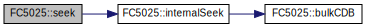
\includegraphics[width=350pt]{classFC5025_ab38385df803acdde0c55e472669ffc2d_cgraph}
\end{center}
\end{figure}


\hypertarget{classFC5025_afff5293f6d1011a7b107607f544fedf5}{}\index{F\+C5025@{F\+C5025}!set\+Density@{set\+Density}}
\index{set\+Density@{set\+Density}!F\+C5025@{F\+C5025}}
\subsubsection[{set\+Density}]{\setlength{\rightskip}{0pt plus 5cm}int F\+C5025\+::set\+Density (
\begin{DoxyParamCaption}
\item[{int}]{density}
\end{DoxyParamCaption}
)}\label{classFC5025_afff5293f6d1011a7b107607f544fedf5}
set density


\begin{DoxyParams}{Parameters}
{\em density} & \\
\hline
\end{DoxyParams}
\begin{DoxyReturn}{Returns}
status 
\end{DoxyReturn}


Definition at line 430 of file fc5025.\+cpp.



Here is the call graph for this function\+:\nopagebreak
\begin{figure}[H]
\begin{center}
\leavevmode
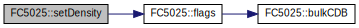
\includegraphics[width=350pt]{classFC5025_afff5293f6d1011a7b107607f544fedf5_cgraph}
\end{center}
\end{figure}




The documentation for this class was generated from the following files\+:\begin{DoxyCompactItemize}
\item 
\hyperlink{fc5025_8h}{fc5025.\+h}\item 
\hyperlink{fc5025_8cpp}{fc5025.\+cpp}\end{DoxyCompactItemize}

\input{classH17Block}
\hypertarget{classH17Disk}{}\section{H17\+Disk Class Reference}
\label{classH17Disk}\index{H17\+Disk@{H17\+Disk}}


Collaboration diagram for H17\+Disk\+:
\nopagebreak
\begin{figure}[H]
\begin{center}
\leavevmode
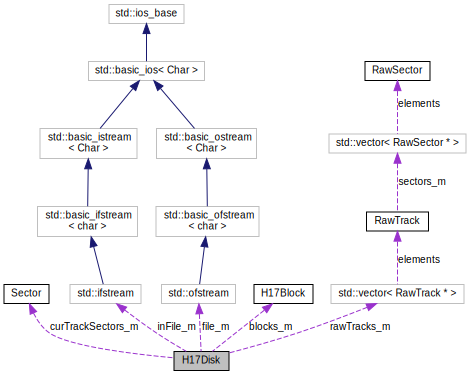
\includegraphics[width=350pt]{classH17Disk__coll__graph}
\end{center}
\end{figure}
\subsection*{Public Member Functions}
\begin{DoxyCompactItemize}
\item 
\hyperlink{classH17Disk_af65aae49c99d4be95b6493b696dbc758}{H17\+Disk} ()
\item 
virtual \hyperlink{classH17Disk_af2d62014dd9e0cdf5604845e1d1f381c}{$\sim$\+H17\+Disk} ()
\item 
virtual bool \hyperlink{classH17Disk_ad29344c720e1a09c4de310d51ce40449}{open\+For\+Write} (char $\ast$name)
\item 
virtual bool \hyperlink{classH17Disk_a2d9e6faca3284d426af174b18554d4a9}{open\+For\+Read} (char $\ast$name)
\item 
virtual bool \hyperlink{classH17Disk_aa375761378f8a80cb8c5e479008c0e32}{open\+For\+Recovery} (char $\ast$name)
\item 
virtual bool \hyperlink{classH17Disk_a8e41c133b13e5c9c2c8f1d39b73d5292}{load\+File} ()
\item 
virtual bool \hyperlink{classH17Disk_adfb88c5c9f3c67a0923a4d24e5efe791}{save\+File} (char $\ast$name)
\item 
virtual bool \hyperlink{classH17Disk_a92edc41852a329daed3e91f50e0271c7}{save\+As\+H8\+D} (char $\ast$name)
\item 
virtual bool \hyperlink{classH17Disk_a0a7412197ca1478393a45885cc132916}{save\+As\+Raw} (char $\ast$name)
\item 
virtual bool \hyperlink{classH17Disk_a0741de759498d3ba29f4bdef4e943590}{load\+Buffer} (unsigned char buf\mbox{[}$\,$\mbox{]}, unsigned int size)
\item 
virtual bool \hyperlink{classH17Disk_a96fe20794510f9235881fd62497f598f}{load\+Header} (unsigned char buf\mbox{[}$\,$\mbox{]}, unsigned int size, unsigned int \&length)
\item 
virtual bool \hyperlink{classH17Disk_ab5299643ce037fb442e0ccb21cb80c5f}{load\+Block} (unsigned char buf\mbox{[}$\,$\mbox{]}, unsigned int size, unsigned int \&length)
\item 
virtual bool \hyperlink{classH17Disk_a4c484465d1c422d5ce5b4661bc72dd3a}{load\+Disk\+Format\+Block} (unsigned char buf\mbox{[}$\,$\mbox{]}, unsigned int size)
\item 
virtual bool \hyperlink{classH17Disk_a8dfa864cc65f81413d3b518c6c1e67e6}{load\+Flags\+Block} (unsigned char buf\mbox{[}$\,$\mbox{]}, unsigned int size)
\item 
virtual bool \hyperlink{classH17Disk_a3a4c239c85de3b29d6d89c8854c8ed9b}{load\+Label\+Block} (unsigned char buf\mbox{[}$\,$\mbox{]}, unsigned int size)
\item 
virtual bool \hyperlink{classH17Disk_a4b28a58f502aedd83052dbbba759ba28}{load\+Comment\+Block} (unsigned char buf\mbox{[}$\,$\mbox{]}, unsigned int size)
\item 
virtual bool \hyperlink{classH17Disk_a06965b624586dda02e6a1cf7ebf53984}{load\+Date\+Block} (unsigned char buf\mbox{[}$\,$\mbox{]}, unsigned int size)
\item 
virtual bool \hyperlink{classH17Disk_a6183e4e35db3b2ae16a9322f377556e4}{load\+Imager\+Block} (unsigned char buf\mbox{[}$\,$\mbox{]}, unsigned int size)
\item 
virtual bool \hyperlink{classH17Disk_aead615d628b0e4c68f69bd746aeabdb1}{load\+Program\+Block} (unsigned char buf\mbox{[}$\,$\mbox{]}, unsigned int size)
\item 
virtual bool \hyperlink{classH17Disk_a36b7999d189ddc7dc05ba9adcbf3b946}{load\+Data\+Block} (unsigned char buf\mbox{[}$\,$\mbox{]}, unsigned int size)
\item 
virtual bool \hyperlink{classH17Disk_a22308e6d39b0bcb15b6234ea12f61a60}{load\+Track\+Block} (unsigned char buf\mbox{[}$\,$\mbox{]}, unsigned int size, unsigned int \&length)
\item 
virtual bool \hyperlink{classH17Disk_ac9e769a95201984cd0dfae38a7a6d80a}{load\+Sector\+Block} (unsigned char buf\mbox{[}$\,$\mbox{]}, unsigned int size, unsigned int \&length)
\item 
virtual bool \hyperlink{classH17Disk_a31ecffc2c61fe921e9a2ef4018ce5c99}{load\+Raw\+Data\+Block} (unsigned char buf\mbox{[}$\,$\mbox{]}, unsigned int size)
\item 
virtual bool \hyperlink{classH17Disk_abc735f36c5a4ab5f1a7d418639fda508}{load\+Raw\+Track\+Block} (unsigned char buf\mbox{[}$\,$\mbox{]}, unsigned int size, unsigned int \&length)
\item 
virtual bool \hyperlink{classH17Disk_a7fc528a2dc311ed9e614a1b212017033}{load\+Raw\+Sector\+Block} (unsigned char buf\mbox{[}$\,$\mbox{]}, unsigned int size, unsigned int \&length)
\item 
virtual bool \hyperlink{classH17Disk_aa6f27c9eaafd2242fd90ff28f19140ca}{analyze} ()
\item 
virtual bool \hyperlink{classH17Disk_a503d2a03bfe0f9bbe3a8bd8dc7d2ec17}{decode\+File} (char $\ast$name)
\item 
virtual bool \hyperlink{classH17Disk_ada058d8b970b4e72569e2fe000817f75}{decode\+Buffer} (unsigned char buf\mbox{[}$\,$\mbox{]}, unsigned int size)
\item 
virtual bool \hyperlink{classH17Disk_ad9402e7823ac0a2741dc316cae361ecd}{validate\+Header} (unsigned char buf\mbox{[}$\,$\mbox{]}, unsigned int size, unsigned int \&length)
\item 
virtual bool \hyperlink{classH17Disk_a29f4d35fba24f0d9cee37bcb02120a6c}{validate\+Block} (unsigned char buf\mbox{[}$\,$\mbox{]}, unsigned int size, unsigned int \&length)
\item 
virtual bool \hyperlink{classH17Disk_aaf268125dfe0bb84c288aff63f5e865d}{validate\+Disk\+Format\+Block} (unsigned char buf\mbox{[}$\,$\mbox{]}, unsigned int size)
\item 
virtual bool \hyperlink{classH17Disk_a676a126b40c2697cbdeb32648a69c15d}{validate\+Flags\+Block} (unsigned char buf\mbox{[}$\,$\mbox{]}, unsigned int size)
\item 
virtual bool \hyperlink{classH17Disk_a80cc18809c189366f4c8ecf494286129}{validate\+Label\+Block} (unsigned char buf\mbox{[}$\,$\mbox{]}, unsigned int size)
\item 
virtual bool \hyperlink{classH17Disk_a0f8be0fb5d8f55eb6843b6668f60facd}{validate\+Comment\+Block} (unsigned char buf\mbox{[}$\,$\mbox{]}, unsigned int size)
\item 
virtual bool \hyperlink{classH17Disk_a08c7c7f0cad0cc24224fc73227b9648e}{validate\+Date\+Block} (unsigned char buf\mbox{[}$\,$\mbox{]}, unsigned int size)
\item 
virtual bool \hyperlink{classH17Disk_a592a6390ad6a382cae246886993954a7}{validate\+Imager\+Block} (unsigned char buf\mbox{[}$\,$\mbox{]}, unsigned int size)
\item 
virtual bool \hyperlink{classH17Disk_adc15505d580fdb29e57c67293d5b3cda}{validate\+Program\+Block} (unsigned char buf\mbox{[}$\,$\mbox{]}, unsigned int size)
\item 
virtual bool \hyperlink{classH17Disk_a593434e6ce0538943cb044b7d0c9c273}{validate\+Data\+Block} (unsigned char buf\mbox{[}$\,$\mbox{]}, unsigned int size)
\item 
virtual bool \hyperlink{classH17Disk_a532c7c77626521afd001ed4a32610912}{validate\+Track\+Block} (unsigned char buf\mbox{[}$\,$\mbox{]}, unsigned int size, unsigned int \&length)
\item 
virtual bool \hyperlink{classH17Disk_a11e3a3c52730f4502a61f69035d7ab38}{validate\+Sector\+Block} (unsigned char buf\mbox{[}$\,$\mbox{]}, unsigned int size, unsigned int \&length)
\item 
virtual bool \hyperlink{classH17Disk_ae1f57f11daa4d4c624d255851838d704}{validate\+Raw\+Data\+Block} (unsigned char buf\mbox{[}$\,$\mbox{]}, unsigned int size)
\item 
virtual bool \hyperlink{classH17Disk_a8f0fa7dbd52e633a2faa267e453cc486}{validate\+Raw\+Track\+Block} (unsigned char buf\mbox{[}$\,$\mbox{]}, unsigned int size, unsigned int \&length)
\item 
virtual bool \hyperlink{classH17Disk_a60b9074cacd5a89f4b8e8dfb37bccf08}{validate\+Raw\+Sector\+Block} (unsigned char buf\mbox{[}$\,$\mbox{]}, unsigned int size, unsigned int \&length)
\item 
virtual void \hyperlink{classH17Disk_a63841bed6a8d9e91a221dc5f72672710}{dump\+Sector\+Header} (unsigned char buf\mbox{[}$\,$\mbox{]})
\item 
virtual void \hyperlink{classH17Disk_a8748c1a43e28a7bb8cea81e837964c54}{dump\+Sector\+Data} (unsigned char buf\mbox{[}$\,$\mbox{]})
\item 
virtual bool \hyperlink{classH17Disk_a6246024e33209823c50cb30d4ea18d2c}{close\+File} (void)
\item 
virtual void \hyperlink{classH17Disk_aadb042dda8ca52912ce9c76aaa7ca9e5}{disable\+Raw} ()
\item 
virtual bool \hyperlink{classH17Disk_a8390bffa0553266decd2e1c21831ea5f}{write\+Header} ()
\item 
virtual bool \hyperlink{classH17Disk_a40df944449f21c6f5319024f0e179f7c}{set\+Sides} (unsigned char sides)
\item 
virtual bool \hyperlink{classH17Disk_a2e492914d9f408f25f1223253d20f5bc}{set\+Tracks} (unsigned char tracks)
\item 
virtual bool \hyperlink{classH17Disk_a888f6eb9e66d45410eb80903df0133d3}{write\+Disk\+Format\+Block} ()
\item 
virtual bool \hyperlink{classH17Disk_aeedd102e18abe2cdcf8630d3cdc5492e}{set\+W\+P\+Parameter} (bool val)
\item 
virtual bool \hyperlink{classH17Disk_a9aaab4accbcfce3205c0eadc9679a9f9}{set\+Distribution\+Parameter} (unsigned char val)
\item 
virtual bool \hyperlink{classH17Disk_adda59abe2fa07a5b565f061346e1439a}{set\+Track\+Data\+Parameter} (unsigned char val)
\item 
virtual bool \hyperlink{classH17Disk_ac4229315d8704036fe339189cbb649cb}{write\+Label} (unsigned char $\ast$buf, uint32\+\_\+t length)
\item 
virtual bool \hyperlink{classH17Disk_a00a11fce25f33fd27437ac32e5f6139a}{write\+Comment} (unsigned char $\ast$buf, uint32\+\_\+t length)
\item 
virtual bool \hyperlink{classH17Disk_ab397651808bc9ffd033584cbe5c1a8be}{write\+Date} (unsigned char $\ast$buf, uint32\+\_\+t length)
\item 
virtual bool \hyperlink{classH17Disk_abed5956f503f0cd51cdb8ebe6cb26c9d}{write\+Imager} (unsigned char $\ast$buf, uint32\+\_\+t length)
\item 
virtual bool \hyperlink{classH17Disk_a71da855358f9c45a027be13ae2009a5e}{write\+Program} (unsigned char $\ast$buf, uint32\+\_\+t length)
\item 
virtual bool \hyperlink{classH17Disk_a678d8b2633be207d5e3879f41991bcf5}{write\+Parameters} ()
\item 
virtual bool \hyperlink{classH17Disk_ae95a1ef9181111102784f12dc00e341b}{start\+Data} ()
\item 
virtual bool \hyperlink{classH17Disk_a0eecc11273d8051ccb68b6975fa55fba}{start\+Track} (unsigned char side, unsigned char track)
\item 
virtual bool \hyperlink{classH17Disk_a1fae79b5db5de046c5d7a2a3d72fcaab}{add\+Sector} (unsigned char sector, unsigned char error, unsigned char $\ast$buf, uint16\+\_\+t length)
\item 
virtual bool \hyperlink{classH17Disk_afd9cbcab815df9a9385ef3864be219e0}{add\+Raw\+Sector} (unsigned char sector, unsigned char $\ast$buf, uint16\+\_\+t length)
\item 
virtual bool \hyperlink{classH17Disk_a4ce50bcef73aef7b49adaeacc9c0990c}{end\+Track} ()
\item 
virtual bool \hyperlink{classH17Disk_a846793318bb41bf41782dd16b156ce14}{end\+Data\+Block} ()
\item 
virtual bool \hyperlink{classH17Disk_a453aedc5aa6cb970c6e174eadb4c6479}{write\+Raw\+Data\+Block} ()
\item 
virtual char $\ast$ \hyperlink{classH17Disk_a0c6e6f10c3dceff61a31827a25e32043}{get\+Sector\+Data} (unsigned char side, unsigned char track, unsigned char sector)
\item 
virtual bool \hyperlink{classH17Disk_a49978c35eab8155da4475519bf5e6e78}{add\+Sector\+To\+Data\+Block} (uint8\+\_\+t side, uint8\+\_\+t track, uint8\+\_\+t sector, uint8\+\_\+t $\ast$buf, uint16\+\_\+t length)
\item 
virtual bool \hyperlink{classH17Disk_a498d909fe673835841cb862efc9d2589}{add\+Raw\+Sector\+To\+Data\+Block} (uint8\+\_\+t side, uint8\+\_\+t track, uint8\+\_\+t sector, uint8\+\_\+t $\ast$buf, uint16\+\_\+t length)
\end{DoxyCompactItemize}
\subsection*{Static Public Attributes}
\begin{DoxyCompactItemize}
\item 
\hypertarget{classH17Disk_a9bbca767478f686785bbb432820103dc}{}static const uint8\+\_\+t {\bfseries Disk\+Format\+Block\+\_\+c} = 0x00\label{classH17Disk_a9bbca767478f686785bbb432820103dc}

\item 
\hypertarget{classH17Disk_a945579b168d52f682d6197f4a00e0693}{}static const uint8\+\_\+t {\bfseries Flags\+Block\+\_\+c} = 0x01\label{classH17Disk_a945579b168d52f682d6197f4a00e0693}

\item 
\hypertarget{classH17Disk_af2b94de0c8f90b5ba6692276c5763bf5}{}static const uint8\+\_\+t {\bfseries Label\+Block\+\_\+c} = 0x02\label{classH17Disk_af2b94de0c8f90b5ba6692276c5763bf5}

\item 
\hypertarget{classH17Disk_ab4e55131dd806954fda38f12c82f4ccd}{}static const uint8\+\_\+t {\bfseries Comment\+Block\+\_\+c} = 0x03\label{classH17Disk_ab4e55131dd806954fda38f12c82f4ccd}

\item 
\hypertarget{classH17Disk_afb42adda895a1c0a2679d1159b203807}{}static const uint8\+\_\+t {\bfseries Date\+Block\+\_\+c} = 0x04\label{classH17Disk_afb42adda895a1c0a2679d1159b203807}

\item 
\hypertarget{classH17Disk_a7d6a12e1f97bdde25bc8acbcd62a9b25}{}static const uint8\+\_\+t {\bfseries Imager\+Block\+\_\+c} = 0x05\label{classH17Disk_a7d6a12e1f97bdde25bc8acbcd62a9b25}

\item 
\hypertarget{classH17Disk_a2930786a1a6aeb478c29e48bf7167875}{}static const uint8\+\_\+t {\bfseries Program\+Block\+\_\+c} = 0x06\label{classH17Disk_a2930786a1a6aeb478c29e48bf7167875}

\item 
\hypertarget{classH17Disk_a718ad42cffb439324ba3b487ca99851b}{}static const uint8\+\_\+t {\bfseries Data\+Block\+\_\+c} = 0x10\label{classH17Disk_a718ad42cffb439324ba3b487ca99851b}

\item 
\hypertarget{classH17Disk_a55eaf676459f71f5509542b6cbf0f0c3}{}static const uint8\+\_\+t {\bfseries Raw\+Data\+Block\+\_\+c} = 0x30\label{classH17Disk_a55eaf676459f71f5509542b6cbf0f0c3}

\item 
\hypertarget{classH17Disk_a302ca6b5d130750da7216c91630374e6}{}static const uint8\+\_\+t {\bfseries Track\+Data\+Id} = 0x11\label{classH17Disk_a302ca6b5d130750da7216c91630374e6}

\item 
\hypertarget{classH17Disk_aef3444308bb936ec9e80cab4b7230b4b}{}static const uint8\+\_\+t {\bfseries Sector\+Data\+Id} = 0x12\label{classH17Disk_aef3444308bb936ec9e80cab4b7230b4b}

\item 
\hypertarget{classH17Disk_a0a408dcfd99d390b9f266fb6db3972a4}{}static const uint8\+\_\+t {\bfseries Raw\+Track\+Data\+Id} = 0x31\label{classH17Disk_a0a408dcfd99d390b9f266fb6db3972a4}

\item 
\hypertarget{classH17Disk_a49f93facafda64ffc06a4a8c428d5986}{}static const uint8\+\_\+t {\bfseries Raw\+Sector\+Data\+Id} = 0x32\label{classH17Disk_a49f93facafda64ffc06a4a8c428d5986}

\item 
\hypertarget{classH17Disk_acd5a918e086c473bfbb792d9e65adfbc}{}static const uint8\+\_\+t {\bfseries Dist\+Unknown} = 0x00\label{classH17Disk_acd5a918e086c473bfbb792d9e65adfbc}

\item 
\hypertarget{classH17Disk_a5ad1666fc009b8d9ef74b4d7c40f3315}{}static const uint8\+\_\+t {\bfseries Distribution\+Disk} = 0x01\label{classH17Disk_a5ad1666fc009b8d9ef74b4d7c40f3315}

\item 
\hypertarget{classH17Disk_ad6726b8fddf981888c09ed73dae7b3a7}{}static const uint8\+\_\+t {\bfseries Working\+Disk} = 0x02\label{classH17Disk_ad6726b8fddf981888c09ed73dae7b3a7}

\item 
\hypertarget{classH17Disk_af68c66fb0b3f8e3bbe017595707775eb}{}static const uint8\+\_\+t {\bfseries Track\+Data\+Unknown} = 0x00\label{classH17Disk_af68c66fb0b3f8e3bbe017595707775eb}

\item 
\hypertarget{classH17Disk_acc335396cc8aad60bd1adb24014ef47d}{}static const uint8\+\_\+t {\bfseries Track\+Data\+Generated\+From\+H8d\+Conversion} = 0x00\label{classH17Disk_acc335396cc8aad60bd1adb24014ef47d}

\item 
\hypertarget{classH17Disk_a34e88c0f1230ed1632b588e5d98844d6}{}static const uint8\+\_\+t {\bfseries Track\+Data\+Created\+On\+Emulator} = 0x01\label{classH17Disk_a34e88c0f1230ed1632b588e5d98844d6}

\item 
\hypertarget{classH17Disk_a3bb6ae30d5b6c2b9332ec999cc4f2f96}{}static const uint8\+\_\+t {\bfseries Track\+Data\+Captured\+On\+H89} = 0x02\label{classH17Disk_a3bb6ae30d5b6c2b9332ec999cc4f2f96}

\item 
\hypertarget{classH17Disk_a8d298ae22c09c87f89a495bcf45ce203}{}static const uint8\+\_\+t {\bfseries Track\+Data\+Captured\+On\+F\+C5025} = 0x03\label{classH17Disk_a8d298ae22c09c87f89a495bcf45ce203}

\item 
\hypertarget{classH17Disk_af29b5cb1331413d4b684ca468179f32f}{}static const uint8\+\_\+t {\bfseries version\+Major\+\_\+c} = 1\label{classH17Disk_af29b5cb1331413d4b684ca468179f32f}

\item 
\hypertarget{classH17Disk_a4e4ed280004572abf1f811fd0c672945}{}static const uint8\+\_\+t {\bfseries version\+Minor\+\_\+c} = 0\label{classH17Disk_a4e4ed280004572abf1f811fd0c672945}

\item 
\hypertarget{classH17Disk_a7597129877594030fab087e982ac4b1a}{}static const uint8\+\_\+t {\bfseries version\+Point\+\_\+c} = 0\label{classH17Disk_a7597129877594030fab087e982ac4b1a}

\end{DoxyCompactItemize}
\subsection*{Private Member Functions}
\begin{DoxyCompactItemize}
\item 
bool \hyperlink{classH17Disk_a988a0510cf62884ebf3dc3fc9c43d0b8}{write\+Block\+Header} (uint8\+\_\+t block\+Id, uint8\+\_\+t flag, uint32\+\_\+t length)
\item 
virtual bool \hyperlink{classH17Disk_a6317e8bd90eed1f3785bcde079c72ae6}{set\+Defaults} ()
\item 
virtual bool \hyperlink{classH17Disk_ad8755a4e016bea07fd30796d7b6c1ca0}{set\+Default\+Disk\+Format} ()
\item 
virtual bool \hyperlink{classH17Disk_a78bd33233d9597f81e69db936efe5356}{set\+Default\+Flags} ()
\end{DoxyCompactItemize}
\subsection*{Private Attributes}
\begin{DoxyCompactItemize}
\item 
\hypertarget{classH17Disk_a71b2b57e3f318205fcfa368046c510a6}{}unsigned char {\bfseries sides\+\_\+m}\label{classH17Disk_a71b2b57e3f318205fcfa368046c510a6}

\item 
\hypertarget{classH17Disk_ab992a0a5a5287a1d94225c5198d473e5}{}unsigned char {\bfseries tracks\+\_\+m}\label{classH17Disk_ab992a0a5a5287a1d94225c5198d473e5}

\item 
\hypertarget{classH17Disk_a3ac5f7c1b2563a8a530a3275c93161b1}{}unsigned char {\bfseries cur\+Side\+\_\+m}\label{classH17Disk_a3ac5f7c1b2563a8a530a3275c93161b1}

\item 
\hypertarget{classH17Disk_aa9e20f2d7324ad9442624cd7d4666769}{}unsigned char {\bfseries cur\+Track\+\_\+m}\label{classH17Disk_aa9e20f2d7324ad9442624cd7d4666769}

\item 
\hypertarget{classH17Disk_a117c856e648d824a935b993dce770eec}{}unsigned char {\bfseries distribution\+\_\+m}\label{classH17Disk_a117c856e648d824a935b993dce770eec}

\item 
\hypertarget{classH17Disk_a6ae4e766c5122aa5f18744f1dbf2c7c4}{}unsigned char {\bfseries track\+Data\+Source\+\_\+m}\label{classH17Disk_a6ae4e766c5122aa5f18744f1dbf2c7c4}

\item 
\hypertarget{classH17Disk_af4c5a9e09f0618ae91f6310bd445ec28}{}bool {\bfseries write\+Protect\+\_\+m}\label{classH17Disk_af4c5a9e09f0618ae91f6310bd445ec28}

\item 
\hypertarget{classH17Disk_a912a1f67ff39154b47b670ac500ec8b7}{}bool {\bfseries disable\+Raw\+\_\+m}\label{classH17Disk_a912a1f67ff39154b47b670ac500ec8b7}

\item 
\hypertarget{classH17Disk_a29e98dea922bdab941b0f427c2f578e5}{}uint8\+\_\+t {\bfseries version\+Major\+\_\+m}\label{classH17Disk_a29e98dea922bdab941b0f427c2f578e5}

\item 
\hypertarget{classH17Disk_a7bc973d0242dc1bdf94cd0a9aadb7670}{}uint8\+\_\+t {\bfseries version\+Minor\+\_\+m}\label{classH17Disk_a7bc973d0242dc1bdf94cd0a9aadb7670}

\item 
\hypertarget{classH17Disk_a6b076c30a6370615424ab9858db65158}{}uint8\+\_\+t {\bfseries version\+Point\+\_\+m}\label{classH17Disk_a6b076c30a6370615424ab9858db65158}

\item 
\hypertarget{classH17Disk_a402b049d3a8b40631f057564d45b0ff6}{}\hyperlink{classH17Block}{H17\+Block} $\ast$ {\bfseries blocks\+\_\+m} \mbox{[}256\mbox{]}\label{classH17Disk_a402b049d3a8b40631f057564d45b0ff6}

\item 
\hypertarget{classH17Disk_a3d0a09a0ffa8b191378fcf7af2340504}{}std\+::ifstream {\bfseries in\+File\+\_\+m}\label{classH17Disk_a3d0a09a0ffa8b191378fcf7af2340504}

\item 
\hypertarget{classH17Disk_a2fbb3e436545a76ac93b2fe4edf9c992}{}std\+::ofstream {\bfseries file\+\_\+m}\label{classH17Disk_a2fbb3e436545a76ac93b2fe4edf9c992}

\item 
\hypertarget{classH17Disk_a5cacf1ebefc3747a7fdd285f39859c4f}{}unsigned int {\bfseries data\+Size\+\_\+m}\label{classH17Disk_a5cacf1ebefc3747a7fdd285f39859c4f}

\item 
\hypertarget{classH17Disk_aee2cc50a379661f551c3c2dc01676320}{}std\+::streampos {\bfseries data\+Block\+Size\+Pos\+\_\+m}\label{classH17Disk_aee2cc50a379661f551c3c2dc01676320}

\item 
\hypertarget{classH17Disk_ae0e2dda11e979df7749be2a6f4090a74}{}std\+::streampos {\bfseries track\+Size\+Pos\+\_\+m}\label{classH17Disk_ae0e2dda11e979df7749be2a6f4090a74}

\item 
\hypertarget{classH17Disk_adbb1ec562a4101fb1e9086e367fc83d6}{}std\+::vector$<$ \hyperlink{classRawTrack}{Raw\+Track} $\ast$ $>$ {\bfseries raw\+Tracks\+\_\+m}\label{classH17Disk_adbb1ec562a4101fb1e9086e367fc83d6}

\item 
\hypertarget{classH17Disk_a49f2f0ec5b217018bd69b4a77d2cd9fa}{}\hyperlink{classSector}{Sector} $\ast$ {\bfseries cur\+Track\+Sectors\+\_\+m} \mbox{[}max\+Sectors\+\_\+c\mbox{]}\label{classH17Disk_a49f2f0ec5b217018bd69b4a77d2cd9fa}

\item 
\hypertarget{classH17Disk_aac87ed97c6b59cd3ba06e3a7dc1a3e29}{}unsigned int {\bfseries sector\+Errs\+\_\+m}\label{classH17Disk_aac87ed97c6b59cd3ba06e3a7dc1a3e29}

\end{DoxyCompactItemize}
\subsection*{Static Private Attributes}
\begin{DoxyCompactItemize}
\item 
\hypertarget{classH17Disk_a7de986f94227f7a2547a66d4417ab59b}{}static const unsigned char {\bfseries max\+Sectors\+\_\+c} = 10\label{classH17Disk_a7de986f94227f7a2547a66d4417ab59b}

\item 
\hypertarget{classH17Disk_a4ffe92b2a4cb611051a262e169ed282e}{}static const uint8\+\_\+t {\bfseries default\+Sides\+\_\+c} = 1\label{classH17Disk_a4ffe92b2a4cb611051a262e169ed282e}

\item 
\hypertarget{classH17Disk_a863d630f06b705a51c4661df1023ca5c}{}static const uint8\+\_\+t {\bfseries default\+Tracks\+\_\+c} = 40\label{classH17Disk_a863d630f06b705a51c4661df1023ca5c}

\end{DoxyCompactItemize}


\subsection{Detailed Description}


Definition at line 18 of file h17disk.\+h.



\subsection{Constructor \& Destructor Documentation}
\hypertarget{classH17Disk_af65aae49c99d4be95b6493b696dbc758}{}\index{H17\+Disk@{H17\+Disk}!H17\+Disk@{H17\+Disk}}
\index{H17\+Disk@{H17\+Disk}!H17\+Disk@{H17\+Disk}}
\subsubsection[{H17\+Disk}]{\setlength{\rightskip}{0pt plus 5cm}H17\+Disk\+::\+H17\+Disk (
\begin{DoxyParamCaption}
{}
\end{DoxyParamCaption}
)}\label{classH17Disk_af65aae49c99d4be95b6493b696dbc758}
Constructor

Defaults to single-\/sided, 40 tracks 

Definition at line 24 of file h17disk.\+cpp.

\hypertarget{classH17Disk_af2d62014dd9e0cdf5604845e1d1f381c}{}\index{H17\+Disk@{H17\+Disk}!````~H17\+Disk@{$\sim$\+H17\+Disk}}
\index{````~H17\+Disk@{$\sim$\+H17\+Disk}!H17\+Disk@{H17\+Disk}}
\subsubsection[{$\sim$\+H17\+Disk}]{\setlength{\rightskip}{0pt plus 5cm}H17\+Disk\+::$\sim$\+H17\+Disk (
\begin{DoxyParamCaption}
{}
\end{DoxyParamCaption}
)\hspace{0.3cm}{\ttfamily [virtual]}}\label{classH17Disk_af2d62014dd9e0cdf5604845e1d1f381c}
destructor 

Definition at line 55 of file h17disk.\+cpp.



\subsection{Member Function Documentation}
\hypertarget{classH17Disk_afd9cbcab815df9a9385ef3864be219e0}{}\index{H17\+Disk@{H17\+Disk}!add\+Raw\+Sector@{add\+Raw\+Sector}}
\index{add\+Raw\+Sector@{add\+Raw\+Sector}!H17\+Disk@{H17\+Disk}}
\subsubsection[{add\+Raw\+Sector}]{\setlength{\rightskip}{0pt plus 5cm}bool H17\+Disk\+::add\+Raw\+Sector (
\begin{DoxyParamCaption}
\item[{unsigned char}]{sector, }
\item[{unsigned char $\ast$}]{buf, }
\item[{uint16\+\_\+t}]{length}
\end{DoxyParamCaption}
)\hspace{0.3cm}{\ttfamily [virtual]}}\label{classH17Disk_afd9cbcab815df9a9385ef3864be219e0}
add raw data sector


\begin{DoxyParams}{Parameters}
{\em sector} & \\
\hline
{\em buf} & \\
\hline
{\em length} & \\
\hline
\end{DoxyParams}
\begin{DoxyReturn}{Returns}
success 
\end{DoxyReturn}


Definition at line 2122 of file h17disk.\+cpp.

\hypertarget{classH17Disk_a498d909fe673835841cb862efc9d2589}{}\index{H17\+Disk@{H17\+Disk}!add\+Raw\+Sector\+To\+Data\+Block@{add\+Raw\+Sector\+To\+Data\+Block}}
\index{add\+Raw\+Sector\+To\+Data\+Block@{add\+Raw\+Sector\+To\+Data\+Block}!H17\+Disk@{H17\+Disk}}
\subsubsection[{add\+Raw\+Sector\+To\+Data\+Block}]{\setlength{\rightskip}{0pt plus 5cm}bool H17\+Disk\+::add\+Raw\+Sector\+To\+Data\+Block (
\begin{DoxyParamCaption}
\item[{uint8\+\_\+t}]{side, }
\item[{uint8\+\_\+t}]{track, }
\item[{uint8\+\_\+t}]{sector, }
\item[{uint8\+\_\+t $\ast$}]{buf, }
\item[{uint16\+\_\+t}]{length}
\end{DoxyParamCaption}
)\hspace{0.3cm}{\ttfamily [virtual]}}\label{classH17Disk_a498d909fe673835841cb862efc9d2589}
add raw sector to data block


\begin{DoxyParams}{Parameters}
{\em side} & \\
\hline
{\em track} & \\
\hline
{\em sector} & \\
\hline
{\em buf} & \\
\hline
{\em length} & \\
\hline
\end{DoxyParams}
\begin{DoxyRefDesc}{Todo}
\item[\hyperlink{todo__todo000012}{Todo}]implememnt \end{DoxyRefDesc}


Definition at line 2176 of file h17disk.\+cpp.

\hypertarget{classH17Disk_a1fae79b5db5de046c5d7a2a3d72fcaab}{}\index{H17\+Disk@{H17\+Disk}!add\+Sector@{add\+Sector}}
\index{add\+Sector@{add\+Sector}!H17\+Disk@{H17\+Disk}}
\subsubsection[{add\+Sector}]{\setlength{\rightskip}{0pt plus 5cm}bool H17\+Disk\+::add\+Sector (
\begin{DoxyParamCaption}
\item[{unsigned char}]{sector, }
\item[{unsigned char}]{error, }
\item[{unsigned char $\ast$}]{buf, }
\item[{uint16\+\_\+t}]{length}
\end{DoxyParamCaption}
)\hspace{0.3cm}{\ttfamily [virtual]}}\label{classH17Disk_a1fae79b5db5de046c5d7a2a3d72fcaab}
add a sector to the track


\begin{DoxyParams}{Parameters}
{\em sector} & \\
\hline
{\em error} & -\/ error code \\
\hline
{\em buf} & -\/ pointer to buffer \\
\hline
{\em length} & -\/ length of buffer\\
\hline
\end{DoxyParams}
\begin{DoxyReturn}{Returns}
success 
\end{DoxyReturn}


Definition at line 1975 of file h17disk.\+cpp.

\hypertarget{classH17Disk_a49978c35eab8155da4475519bf5e6e78}{}\index{H17\+Disk@{H17\+Disk}!add\+Sector\+To\+Data\+Block@{add\+Sector\+To\+Data\+Block}}
\index{add\+Sector\+To\+Data\+Block@{add\+Sector\+To\+Data\+Block}!H17\+Disk@{H17\+Disk}}
\subsubsection[{add\+Sector\+To\+Data\+Block}]{\setlength{\rightskip}{0pt plus 5cm}bool H17\+Disk\+::add\+Sector\+To\+Data\+Block (
\begin{DoxyParamCaption}
\item[{uint8\+\_\+t}]{side, }
\item[{uint8\+\_\+t}]{track, }
\item[{uint8\+\_\+t}]{sector, }
\item[{uint8\+\_\+t $\ast$}]{buf, }
\item[{uint16\+\_\+t}]{length}
\end{DoxyParamCaption}
)\hspace{0.3cm}{\ttfamily [virtual]}}\label{classH17Disk_a49978c35eab8155da4475519bf5e6e78}
add sector to data block


\begin{DoxyParams}{Parameters}
{\em side} & \\
\hline
{\em track} & \\
\hline
{\em sector} & \\
\hline
{\em buf} & \\
\hline
{\em length} & \\
\hline
\end{DoxyParams}
\begin{DoxyRefDesc}{Todo}
\item[\hyperlink{todo__todo000011}{Todo}]implememnt \end{DoxyRefDesc}


Definition at line 2149 of file h17disk.\+cpp.

\hypertarget{classH17Disk_aa6f27c9eaafd2242fd90ff28f19140ca}{}\index{H17\+Disk@{H17\+Disk}!analyze@{analyze}}
\index{analyze@{analyze}!H17\+Disk@{H17\+Disk}}
\subsubsection[{analyze}]{\setlength{\rightskip}{0pt plus 5cm}bool H17\+Disk\+::analyze (
\begin{DoxyParamCaption}
{}
\end{DoxyParamCaption}
)\hspace{0.3cm}{\ttfamily [virtual]}}\label{classH17Disk_aa6f27c9eaafd2242fd90ff28f19140ca}
analyze the disk image

\begin{DoxyReturn}{Returns}
success 
\end{DoxyReturn}


Definition at line 268 of file h17disk.\+cpp.

\hypertarget{classH17Disk_a6246024e33209823c50cb30d4ea18d2c}{}\index{H17\+Disk@{H17\+Disk}!close\+File@{close\+File}}
\index{close\+File@{close\+File}!H17\+Disk@{H17\+Disk}}
\subsubsection[{close\+File}]{\setlength{\rightskip}{0pt plus 5cm}bool H17\+Disk\+::close\+File (
\begin{DoxyParamCaption}
\item[{void}]{}
\end{DoxyParamCaption}
)\hspace{0.3cm}{\ttfamily [virtual]}}\label{classH17Disk_a6246024e33209823c50cb30d4ea18d2c}
close file

\begin{DoxyReturn}{Returns}
success 
\end{DoxyReturn}


Definition at line 1763 of file h17disk.\+cpp.

\hypertarget{classH17Disk_ada058d8b970b4e72569e2fe000817f75}{}\index{H17\+Disk@{H17\+Disk}!decode\+Buffer@{decode\+Buffer}}
\index{decode\+Buffer@{decode\+Buffer}!H17\+Disk@{H17\+Disk}}
\subsubsection[{decode\+Buffer}]{\setlength{\rightskip}{0pt plus 5cm}bool H17\+Disk\+::decode\+Buffer (
\begin{DoxyParamCaption}
\item[{unsigned char}]{buf\mbox{[}$\,$\mbox{]}, }
\item[{unsigned int}]{size}
\end{DoxyParamCaption}
)\hspace{0.3cm}{\ttfamily [virtual]}}\label{classH17Disk_ada058d8b970b4e72569e2fe000817f75}
decodes memory buffer of a h17disk file


\begin{DoxyParams}{Parameters}
{\em buf} & \\
\hline
{\em size} & \\
\hline
\end{DoxyParams}
\begin{DoxyReturn}{Returns}
success 
\end{DoxyReturn}


Definition at line 340 of file h17disk.\+cpp.



Here is the call graph for this function\+:
\nopagebreak
\begin{figure}[H]
\begin{center}
\leavevmode
\includegraphics[width=350pt]{classH17Disk_ada058d8b970b4e72569e2fe000817f75_cgraph}
\end{center}
\end{figure}




Here is the caller graph for this function\+:
\nopagebreak
\begin{figure}[H]
\begin{center}
\leavevmode
\includegraphics[width=343pt]{classH17Disk_ada058d8b970b4e72569e2fe000817f75_icgraph}
\end{center}
\end{figure}


\hypertarget{classH17Disk_a503d2a03bfe0f9bbe3a8bd8dc7d2ec17}{}\index{H17\+Disk@{H17\+Disk}!decode\+File@{decode\+File}}
\index{decode\+File@{decode\+File}!H17\+Disk@{H17\+Disk}}
\subsubsection[{decode\+File}]{\setlength{\rightskip}{0pt plus 5cm}bool H17\+Disk\+::decode\+File (
\begin{DoxyParamCaption}
\item[{char $\ast$}]{name}
\end{DoxyParamCaption}
)\hspace{0.3cm}{\ttfamily [virtual]}}\label{classH17Disk_a503d2a03bfe0f9bbe3a8bd8dc7d2ec17}
decode file and dump results to screen


\begin{DoxyParams}{Parameters}
{\em name} & file name\\
\hline
\end{DoxyParams}
\begin{DoxyReturn}{Returns}
success 
\end{DoxyReturn}


Definition at line 306 of file h17disk.\+cpp.



Here is the call graph for this function\+:
\nopagebreak
\begin{figure}[H]
\begin{center}
\leavevmode
\includegraphics[width=350pt]{classH17Disk_a503d2a03bfe0f9bbe3a8bd8dc7d2ec17_cgraph}
\end{center}
\end{figure}


\hypertarget{classH17Disk_aadb042dda8ca52912ce9c76aaa7ca9e5}{}\index{H17\+Disk@{H17\+Disk}!disable\+Raw@{disable\+Raw}}
\index{disable\+Raw@{disable\+Raw}!H17\+Disk@{H17\+Disk}}
\subsubsection[{disable\+Raw}]{\setlength{\rightskip}{0pt plus 5cm}void H17\+Disk\+::disable\+Raw (
\begin{DoxyParamCaption}
{}
\end{DoxyParamCaption}
)\hspace{0.3cm}{\ttfamily [virtual]}}\label{classH17Disk_aadb042dda8ca52912ce9c76aaa7ca9e5}
disable raw blocks 

Definition at line 72 of file h17disk.\+cpp.

\hypertarget{classH17Disk_a8748c1a43e28a7bb8cea81e837964c54}{}\index{H17\+Disk@{H17\+Disk}!dump\+Sector\+Data@{dump\+Sector\+Data}}
\index{dump\+Sector\+Data@{dump\+Sector\+Data}!H17\+Disk@{H17\+Disk}}
\subsubsection[{dump\+Sector\+Data}]{\setlength{\rightskip}{0pt plus 5cm}void H17\+Disk\+::dump\+Sector\+Data (
\begin{DoxyParamCaption}
\item[{unsigned char}]{buf\mbox{[}$\,$\mbox{]}}
\end{DoxyParamCaption}
)\hspace{0.3cm}{\ttfamily [virtual]}}\label{classH17Disk_a8748c1a43e28a7bb8cea81e837964c54}
dump Sector\+Data


\begin{DoxyParams}{Parameters}
{\em buf} & data buffer \\
\hline
\end{DoxyParams}


Definition at line 1343 of file h17disk.\+cpp.



Here is the caller graph for this function\+:
\nopagebreak
\begin{figure}[H]
\begin{center}
\leavevmode
\includegraphics[width=350pt]{classH17Disk_a8748c1a43e28a7bb8cea81e837964c54_icgraph}
\end{center}
\end{figure}


\hypertarget{classH17Disk_a63841bed6a8d9e91a221dc5f72672710}{}\index{H17\+Disk@{H17\+Disk}!dump\+Sector\+Header@{dump\+Sector\+Header}}
\index{dump\+Sector\+Header@{dump\+Sector\+Header}!H17\+Disk@{H17\+Disk}}
\subsubsection[{dump\+Sector\+Header}]{\setlength{\rightskip}{0pt plus 5cm}void H17\+Disk\+::dump\+Sector\+Header (
\begin{DoxyParamCaption}
\item[{unsigned char}]{buf\mbox{[}$\,$\mbox{]}}
\end{DoxyParamCaption}
)\hspace{0.3cm}{\ttfamily [virtual]}}\label{classH17Disk_a63841bed6a8d9e91a221dc5f72672710}
dump Sector\+Header


\begin{DoxyParams}{Parameters}
{\em buf} & data buffer \\
\hline
\end{DoxyParams}


Definition at line 1328 of file h17disk.\+cpp.



Here is the caller graph for this function\+:
\nopagebreak
\begin{figure}[H]
\begin{center}
\leavevmode
\includegraphics[width=350pt]{classH17Disk_a63841bed6a8d9e91a221dc5f72672710_icgraph}
\end{center}
\end{figure}


\hypertarget{classH17Disk_a846793318bb41bf41782dd16b156ce14}{}\index{H17\+Disk@{H17\+Disk}!end\+Data\+Block@{end\+Data\+Block}}
\index{end\+Data\+Block@{end\+Data\+Block}!H17\+Disk@{H17\+Disk}}
\subsubsection[{end\+Data\+Block}]{\setlength{\rightskip}{0pt plus 5cm}bool H17\+Disk\+::end\+Data\+Block (
\begin{DoxyParamCaption}
{}
\end{DoxyParamCaption}
)\hspace{0.3cm}{\ttfamily [virtual]}}\label{classH17Disk_a846793318bb41bf41782dd16b156ce14}
end data block and update size

\begin{DoxyReturn}{Returns}
success 
\end{DoxyReturn}


Definition at line 2048 of file h17disk.\+cpp.

\hypertarget{classH17Disk_a4ce50bcef73aef7b49adaeacc9c0990c}{}\index{H17\+Disk@{H17\+Disk}!end\+Track@{end\+Track}}
\index{end\+Track@{end\+Track}!H17\+Disk@{H17\+Disk}}
\subsubsection[{end\+Track}]{\setlength{\rightskip}{0pt plus 5cm}bool H17\+Disk\+::end\+Track (
\begin{DoxyParamCaption}
{}
\end{DoxyParamCaption}
)\hspace{0.3cm}{\ttfamily [virtual]}}\label{classH17Disk_a4ce50bcef73aef7b49adaeacc9c0990c}
end track and update size of track

\begin{DoxyReturn}{Returns}
success 
\end{DoxyReturn}


Definition at line 2000 of file h17disk.\+cpp.



Here is the call graph for this function\+:
\nopagebreak
\begin{figure}[H]
\begin{center}
\leavevmode
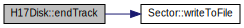
\includegraphics[width=316pt]{classH17Disk_a4ce50bcef73aef7b49adaeacc9c0990c_cgraph}
\end{center}
\end{figure}


\hypertarget{classH17Disk_a0c6e6f10c3dceff61a31827a25e32043}{}\index{H17\+Disk@{H17\+Disk}!get\+Sector\+Data@{get\+Sector\+Data}}
\index{get\+Sector\+Data@{get\+Sector\+Data}!H17\+Disk@{H17\+Disk}}
\subsubsection[{get\+Sector\+Data}]{\setlength{\rightskip}{0pt plus 5cm}char $\ast$ H17\+Disk\+::get\+Sector\+Data (
\begin{DoxyParamCaption}
\item[{unsigned char}]{side, }
\item[{unsigned char}]{track, }
\item[{unsigned char}]{sector}
\end{DoxyParamCaption}
)\hspace{0.3cm}{\ttfamily [virtual]}}\label{classH17Disk_a0c6e6f10c3dceff61a31827a25e32043}
get sector data


\begin{DoxyParams}{Parameters}
{\em side} & \\
\hline
{\em track} & \\
\hline
{\em sector} & \\
\hline
\end{DoxyParams}
\begin{DoxyReturn}{Returns}
pointer to buffer
\end{DoxyReturn}
\begin{DoxyRefDesc}{Todo}
\item[\hyperlink{todo__todo000013}{Todo}]needs to return both the pointer and length. 

implememnt \end{DoxyRefDesc}


Definition at line 2204 of file h17disk.\+cpp.

\hypertarget{classH17Disk_ab5299643ce037fb442e0ccb21cb80c5f}{}\index{H17\+Disk@{H17\+Disk}!load\+Block@{load\+Block}}
\index{load\+Block@{load\+Block}!H17\+Disk@{H17\+Disk}}
\subsubsection[{load\+Block}]{\setlength{\rightskip}{0pt plus 5cm}bool H17\+Disk\+::load\+Block (
\begin{DoxyParamCaption}
\item[{unsigned char}]{buf\mbox{[}$\,$\mbox{]}, }
\item[{unsigned int}]{size, }
\item[{unsigned int \&}]{length}
\end{DoxyParamCaption}
)\hspace{0.3cm}{\ttfamily [virtual]}}\label{classH17Disk_ab5299643ce037fb442e0ccb21cb80c5f}
load block


\begin{DoxyParams}{Parameters}
{\em buf} & data buffer \\
\hline
{\em size} & size of buffer \\
\hline
{\em } & \\
\hline
\end{DoxyParams}
\begin{DoxyRefDesc}{Todo}
\item[\hyperlink{todo__todo000010}{Todo}]check to see if mandatory , and skip the data. \end{DoxyRefDesc}


Definition at line 563 of file h17disk.\+cpp.



Here is the call graph for this function\+:
\nopagebreak
\begin{figure}[H]
\begin{center}
\leavevmode
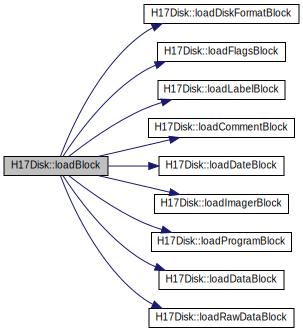
\includegraphics[width=350pt]{classH17Disk_ab5299643ce037fb442e0ccb21cb80c5f_cgraph}
\end{center}
\end{figure}




Here is the caller graph for this function\+:
\nopagebreak
\begin{figure}[H]
\begin{center}
\leavevmode
\includegraphics[width=350pt]{classH17Disk_ab5299643ce037fb442e0ccb21cb80c5f_icgraph}
\end{center}
\end{figure}


\hypertarget{classH17Disk_a0741de759498d3ba29f4bdef4e943590}{}\index{H17\+Disk@{H17\+Disk}!load\+Buffer@{load\+Buffer}}
\index{load\+Buffer@{load\+Buffer}!H17\+Disk@{H17\+Disk}}
\subsubsection[{load\+Buffer}]{\setlength{\rightskip}{0pt plus 5cm}bool H17\+Disk\+::load\+Buffer (
\begin{DoxyParamCaption}
\item[{unsigned char}]{buf\mbox{[}$\,$\mbox{]}, }
\item[{unsigned int}]{size}
\end{DoxyParamCaption}
)\hspace{0.3cm}{\ttfamily [virtual]}}\label{classH17Disk_a0741de759498d3ba29f4bdef4e943590}
load buffer into a h17disk object


\begin{DoxyParams}{Parameters}
{\em buf} & \\
\hline
{\em size} & \\
\hline
\end{DoxyParams}
\begin{DoxyReturn}{Returns}
success 
\end{DoxyReturn}


Definition at line 375 of file h17disk.\+cpp.



Here is the call graph for this function\+:
\nopagebreak
\begin{figure}[H]
\begin{center}
\leavevmode
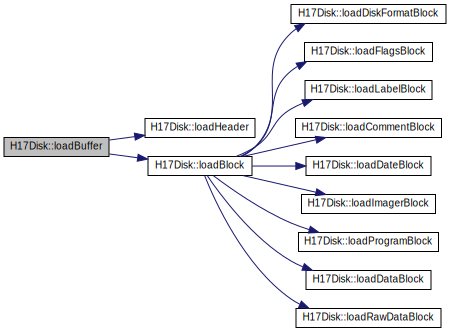
\includegraphics[width=350pt]{classH17Disk_a0741de759498d3ba29f4bdef4e943590_cgraph}
\end{center}
\end{figure}




Here is the caller graph for this function\+:
\nopagebreak
\begin{figure}[H]
\begin{center}
\leavevmode
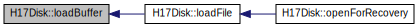
\includegraphics[width=350pt]{classH17Disk_a0741de759498d3ba29f4bdef4e943590_icgraph}
\end{center}
\end{figure}


\hypertarget{classH17Disk_a4b28a58f502aedd83052dbbba759ba28}{}\index{H17\+Disk@{H17\+Disk}!load\+Comment\+Block@{load\+Comment\+Block}}
\index{load\+Comment\+Block@{load\+Comment\+Block}!H17\+Disk@{H17\+Disk}}
\subsubsection[{load\+Comment\+Block}]{\setlength{\rightskip}{0pt plus 5cm}bool H17\+Disk\+::load\+Comment\+Block (
\begin{DoxyParamCaption}
\item[{unsigned char}]{buf\mbox{[}$\,$\mbox{]}, }
\item[{unsigned int}]{size}
\end{DoxyParamCaption}
)\hspace{0.3cm}{\ttfamily [virtual]}}\label{classH17Disk_a4b28a58f502aedd83052dbbba759ba28}
load Comment\+Block


\begin{DoxyParams}{Parameters}
{\em buf} & data buffer \\
\hline
{\em size} & size of buffer\\
\hline
\end{DoxyParams}
\begin{DoxyReturn}{Returns}
if load was successful 
\end{DoxyReturn}


Definition at line 761 of file h17disk.\+cpp.



Here is the caller graph for this function\+:
\nopagebreak
\begin{figure}[H]
\begin{center}
\leavevmode
\includegraphics[width=350pt]{classH17Disk_a4b28a58f502aedd83052dbbba759ba28_icgraph}
\end{center}
\end{figure}


\hypertarget{classH17Disk_a36b7999d189ddc7dc05ba9adcbf3b946}{}\index{H17\+Disk@{H17\+Disk}!load\+Data\+Block@{load\+Data\+Block}}
\index{load\+Data\+Block@{load\+Data\+Block}!H17\+Disk@{H17\+Disk}}
\subsubsection[{load\+Data\+Block}]{\setlength{\rightskip}{0pt plus 5cm}bool H17\+Disk\+::load\+Data\+Block (
\begin{DoxyParamCaption}
\item[{unsigned char}]{buf\mbox{[}$\,$\mbox{]}, }
\item[{unsigned int}]{size}
\end{DoxyParamCaption}
)\hspace{0.3cm}{\ttfamily [virtual]}}\label{classH17Disk_a36b7999d189ddc7dc05ba9adcbf3b946}
load Data\+Block


\begin{DoxyParams}{Parameters}
{\em buf} & data buffer \\
\hline
{\em size} & size of buffer\\
\hline
\end{DoxyParams}
\begin{DoxyReturn}{Returns}
if load was successful 
\end{DoxyReturn}


Definition at line 1034 of file h17disk.\+cpp.



Here is the caller graph for this function\+:
\nopagebreak
\begin{figure}[H]
\begin{center}
\leavevmode
\includegraphics[width=350pt]{classH17Disk_a36b7999d189ddc7dc05ba9adcbf3b946_icgraph}
\end{center}
\end{figure}


\hypertarget{classH17Disk_a06965b624586dda02e6a1cf7ebf53984}{}\index{H17\+Disk@{H17\+Disk}!load\+Date\+Block@{load\+Date\+Block}}
\index{load\+Date\+Block@{load\+Date\+Block}!H17\+Disk@{H17\+Disk}}
\subsubsection[{load\+Date\+Block}]{\setlength{\rightskip}{0pt plus 5cm}bool H17\+Disk\+::load\+Date\+Block (
\begin{DoxyParamCaption}
\item[{unsigned char}]{buf\mbox{[}$\,$\mbox{]}, }
\item[{unsigned int}]{size}
\end{DoxyParamCaption}
)\hspace{0.3cm}{\ttfamily [virtual]}}\label{classH17Disk_a06965b624586dda02e6a1cf7ebf53984}
load Date\+Block


\begin{DoxyParams}{Parameters}
{\em buf} & data buffer \\
\hline
{\em size} & size of buffer\\
\hline
\end{DoxyParams}
\begin{DoxyReturn}{Returns}
if load was successful 
\end{DoxyReturn}


Definition at line 811 of file h17disk.\+cpp.



Here is the caller graph for this function\+:
\nopagebreak
\begin{figure}[H]
\begin{center}
\leavevmode
\includegraphics[width=350pt]{classH17Disk_a06965b624586dda02e6a1cf7ebf53984_icgraph}
\end{center}
\end{figure}


\hypertarget{classH17Disk_a4c484465d1c422d5ce5b4661bc72dd3a}{}\index{H17\+Disk@{H17\+Disk}!load\+Disk\+Format\+Block@{load\+Disk\+Format\+Block}}
\index{load\+Disk\+Format\+Block@{load\+Disk\+Format\+Block}!H17\+Disk@{H17\+Disk}}
\subsubsection[{load\+Disk\+Format\+Block}]{\setlength{\rightskip}{0pt plus 5cm}bool H17\+Disk\+::load\+Disk\+Format\+Block (
\begin{DoxyParamCaption}
\item[{unsigned char}]{buf\mbox{[}$\,$\mbox{]}, }
\item[{unsigned int}]{size}
\end{DoxyParamCaption}
)\hspace{0.3cm}{\ttfamily [virtual]}}\label{classH17Disk_a4c484465d1c422d5ce5b4661bc72dd3a}
Load Disk\+Format\+Block


\begin{DoxyParams}{Parameters}
{\em buf} & data buffer \\
\hline
{\em size} & size of buffer\\
\hline
\end{DoxyParams}
\begin{DoxyReturn}{Returns}
if validation was succesful 
\end{DoxyReturn}


Definition at line 660 of file h17disk.\+cpp.



Here is the caller graph for this function\+:
\nopagebreak
\begin{figure}[H]
\begin{center}
\leavevmode
\includegraphics[width=350pt]{classH17Disk_a4c484465d1c422d5ce5b4661bc72dd3a_icgraph}
\end{center}
\end{figure}


\hypertarget{classH17Disk_a8e41c133b13e5c9c2c8f1d39b73d5292}{}\index{H17\+Disk@{H17\+Disk}!load\+File@{load\+File}}
\index{load\+File@{load\+File}!H17\+Disk@{H17\+Disk}}
\subsubsection[{load\+File}]{\setlength{\rightskip}{0pt plus 5cm}bool H17\+Disk\+::load\+File (
\begin{DoxyParamCaption}
{}
\end{DoxyParamCaption}
)\hspace{0.3cm}{\ttfamily [virtual]}}\label{classH17Disk_a8e41c133b13e5c9c2c8f1d39b73d5292}
load file after in\+File\+\_\+m has been opened

\begin{DoxyReturn}{Returns}
success 
\end{DoxyReturn}


Definition at line 148 of file h17disk.\+cpp.



Here is the call graph for this function\+:
\nopagebreak
\begin{figure}[H]
\begin{center}
\leavevmode
\includegraphics[width=350pt]{classH17Disk_a8e41c133b13e5c9c2c8f1d39b73d5292_cgraph}
\end{center}
\end{figure}




Here is the caller graph for this function\+:
\nopagebreak
\begin{figure}[H]
\begin{center}
\leavevmode
\includegraphics[width=349pt]{classH17Disk_a8e41c133b13e5c9c2c8f1d39b73d5292_icgraph}
\end{center}
\end{figure}


\hypertarget{classH17Disk_a8dfa864cc65f81413d3b518c6c1e67e6}{}\index{H17\+Disk@{H17\+Disk}!load\+Flags\+Block@{load\+Flags\+Block}}
\index{load\+Flags\+Block@{load\+Flags\+Block}!H17\+Disk@{H17\+Disk}}
\subsubsection[{load\+Flags\+Block}]{\setlength{\rightskip}{0pt plus 5cm}bool H17\+Disk\+::load\+Flags\+Block (
\begin{DoxyParamCaption}
\item[{unsigned char}]{buf\mbox{[}$\,$\mbox{]}, }
\item[{unsigned int}]{size}
\end{DoxyParamCaption}
)\hspace{0.3cm}{\ttfamily [virtual]}}\label{classH17Disk_a8dfa864cc65f81413d3b518c6c1e67e6}
load Flags\+Block


\begin{DoxyParams}{Parameters}
{\em buf} & data buffer \\
\hline
{\em size} & size of buffer\\
\hline
\end{DoxyParams}
\begin{DoxyReturn}{Returns}
if load was successful 
\end{DoxyReturn}


Definition at line 970 of file h17disk.\+cpp.



Here is the caller graph for this function\+:
\nopagebreak
\begin{figure}[H]
\begin{center}
\leavevmode
\includegraphics[width=350pt]{classH17Disk_a8dfa864cc65f81413d3b518c6c1e67e6_icgraph}
\end{center}
\end{figure}


\hypertarget{classH17Disk_a96fe20794510f9235881fd62497f598f}{}\index{H17\+Disk@{H17\+Disk}!load\+Header@{load\+Header}}
\index{load\+Header@{load\+Header}!H17\+Disk@{H17\+Disk}}
\subsubsection[{load\+Header}]{\setlength{\rightskip}{0pt plus 5cm}bool H17\+Disk\+::load\+Header (
\begin{DoxyParamCaption}
\item[{unsigned char}]{buf\mbox{[}$\,$\mbox{]}, }
\item[{unsigned int}]{size, }
\item[{unsigned int \&}]{length}
\end{DoxyParamCaption}
)\hspace{0.3cm}{\ttfamily [virtual]}}\label{classH17Disk_a96fe20794510f9235881fd62497f598f}
load header of h17disk file


\begin{DoxyParams}{Parameters}
{\em buf} & data buffer \\
\hline
{\em size} & size of buffer \\
\hline
{\em } & \\
\hline
\end{DoxyParams}


Definition at line 454 of file h17disk.\+cpp.



Here is the caller graph for this function\+:
\nopagebreak
\begin{figure}[H]
\begin{center}
\leavevmode
\includegraphics[width=350pt]{classH17Disk_a96fe20794510f9235881fd62497f598f_icgraph}
\end{center}
\end{figure}


\hypertarget{classH17Disk_a6183e4e35db3b2ae16a9322f377556e4}{}\index{H17\+Disk@{H17\+Disk}!load\+Imager\+Block@{load\+Imager\+Block}}
\index{load\+Imager\+Block@{load\+Imager\+Block}!H17\+Disk@{H17\+Disk}}
\subsubsection[{load\+Imager\+Block}]{\setlength{\rightskip}{0pt plus 5cm}bool H17\+Disk\+::load\+Imager\+Block (
\begin{DoxyParamCaption}
\item[{unsigned char}]{buf\mbox{[}$\,$\mbox{]}, }
\item[{unsigned int}]{size}
\end{DoxyParamCaption}
)\hspace{0.3cm}{\ttfamily [virtual]}}\label{classH17Disk_a6183e4e35db3b2ae16a9322f377556e4}
load Imager\+Block


\begin{DoxyParams}{Parameters}
{\em buf} & data buffer \\
\hline
{\em size} & size of buffer\\
\hline
\end{DoxyParams}
\begin{DoxyReturn}{Returns}
if load was successful 
\end{DoxyReturn}


Definition at line 860 of file h17disk.\+cpp.



Here is the caller graph for this function\+:
\nopagebreak
\begin{figure}[H]
\begin{center}
\leavevmode
\includegraphics[width=350pt]{classH17Disk_a6183e4e35db3b2ae16a9322f377556e4_icgraph}
\end{center}
\end{figure}


\hypertarget{classH17Disk_a3a4c239c85de3b29d6d89c8854c8ed9b}{}\index{H17\+Disk@{H17\+Disk}!load\+Label\+Block@{load\+Label\+Block}}
\index{load\+Label\+Block@{load\+Label\+Block}!H17\+Disk@{H17\+Disk}}
\subsubsection[{load\+Label\+Block}]{\setlength{\rightskip}{0pt plus 5cm}bool H17\+Disk\+::load\+Label\+Block (
\begin{DoxyParamCaption}
\item[{unsigned char}]{buf\mbox{[}$\,$\mbox{]}, }
\item[{unsigned int}]{size}
\end{DoxyParamCaption}
)\hspace{0.3cm}{\ttfamily [virtual]}}\label{classH17Disk_a3a4c239c85de3b29d6d89c8854c8ed9b}
load Label\+Block


\begin{DoxyParams}{Parameters}
{\em buf} & data buffer \\
\hline
{\em size} & size of buffer\\
\hline
\end{DoxyParams}
\begin{DoxyReturn}{Returns}
if load was successful 
\end{DoxyReturn}


Definition at line 711 of file h17disk.\+cpp.



Here is the caller graph for this function\+:
\nopagebreak
\begin{figure}[H]
\begin{center}
\leavevmode
\includegraphics[width=350pt]{classH17Disk_a3a4c239c85de3b29d6d89c8854c8ed9b_icgraph}
\end{center}
\end{figure}


\hypertarget{classH17Disk_aead615d628b0e4c68f69bd746aeabdb1}{}\index{H17\+Disk@{H17\+Disk}!load\+Program\+Block@{load\+Program\+Block}}
\index{load\+Program\+Block@{load\+Program\+Block}!H17\+Disk@{H17\+Disk}}
\subsubsection[{load\+Program\+Block}]{\setlength{\rightskip}{0pt plus 5cm}bool H17\+Disk\+::load\+Program\+Block (
\begin{DoxyParamCaption}
\item[{unsigned char}]{buf\mbox{[}$\,$\mbox{]}, }
\item[{unsigned int}]{size}
\end{DoxyParamCaption}
)\hspace{0.3cm}{\ttfamily [virtual]}}\label{classH17Disk_aead615d628b0e4c68f69bd746aeabdb1}
load Program\+Block


\begin{DoxyParams}{Parameters}
{\em buf} & data buffer \\
\hline
{\em size} & size of buffer\\
\hline
\end{DoxyParams}
\begin{DoxyReturn}{Returns}
if load was successful 
\end{DoxyReturn}


Definition at line 910 of file h17disk.\+cpp.



Here is the caller graph for this function\+:
\nopagebreak
\begin{figure}[H]
\begin{center}
\leavevmode
\includegraphics[width=350pt]{classH17Disk_aead615d628b0e4c68f69bd746aeabdb1_icgraph}
\end{center}
\end{figure}


\hypertarget{classH17Disk_a31ecffc2c61fe921e9a2ef4018ce5c99}{}\index{H17\+Disk@{H17\+Disk}!load\+Raw\+Data\+Block@{load\+Raw\+Data\+Block}}
\index{load\+Raw\+Data\+Block@{load\+Raw\+Data\+Block}!H17\+Disk@{H17\+Disk}}
\subsubsection[{load\+Raw\+Data\+Block}]{\setlength{\rightskip}{0pt plus 5cm}bool H17\+Disk\+::load\+Raw\+Data\+Block (
\begin{DoxyParamCaption}
\item[{unsigned char}]{buf\mbox{[}$\,$\mbox{]}, }
\item[{unsigned int}]{size}
\end{DoxyParamCaption}
)\hspace{0.3cm}{\ttfamily [virtual]}}\label{classH17Disk_a31ecffc2c61fe921e9a2ef4018ce5c99}
load Raw\+Data\+Block


\begin{DoxyParams}{Parameters}
{\em buf} & data buffer \\
\hline
{\em size} & size of buffer\\
\hline
\end{DoxyParams}
\begin{DoxyReturn}{Returns}
if load was successful 
\end{DoxyReturn}


Definition at line 1426 of file h17disk.\+cpp.



Here is the caller graph for this function\+:
\nopagebreak
\begin{figure}[H]
\begin{center}
\leavevmode
\includegraphics[width=350pt]{classH17Disk_a31ecffc2c61fe921e9a2ef4018ce5c99_icgraph}
\end{center}
\end{figure}


\hypertarget{classH17Disk_a7fc528a2dc311ed9e614a1b212017033}{}\index{H17\+Disk@{H17\+Disk}!load\+Raw\+Sector\+Block@{load\+Raw\+Sector\+Block}}
\index{load\+Raw\+Sector\+Block@{load\+Raw\+Sector\+Block}!H17\+Disk@{H17\+Disk}}
\subsubsection[{load\+Raw\+Sector\+Block}]{\setlength{\rightskip}{0pt plus 5cm}bool H17\+Disk\+::load\+Raw\+Sector\+Block (
\begin{DoxyParamCaption}
\item[{unsigned char}]{buf\mbox{[}$\,$\mbox{]}, }
\item[{unsigned int}]{size, }
\item[{unsigned int \&}]{length}
\end{DoxyParamCaption}
)\hspace{0.3cm}{\ttfamily [virtual]}}\label{classH17Disk_a7fc528a2dc311ed9e614a1b212017033}
load raw sector block


\begin{DoxyParams}{Parameters}
{\em buf} & \\
\hline
{\em size} & \\
\hline
{\em length} & \\
\hline
\end{DoxyParams}
\begin{DoxyReturn}{Returns}
success 
\end{DoxyReturn}


Definition at line 1608 of file h17disk.\+cpp.

\hypertarget{classH17Disk_abc735f36c5a4ab5f1a7d418639fda508}{}\index{H17\+Disk@{H17\+Disk}!load\+Raw\+Track\+Block@{load\+Raw\+Track\+Block}}
\index{load\+Raw\+Track\+Block@{load\+Raw\+Track\+Block}!H17\+Disk@{H17\+Disk}}
\subsubsection[{load\+Raw\+Track\+Block}]{\setlength{\rightskip}{0pt plus 5cm}bool H17\+Disk\+::load\+Raw\+Track\+Block (
\begin{DoxyParamCaption}
\item[{unsigned char}]{buf\mbox{[}$\,$\mbox{]}, }
\item[{unsigned int}]{size, }
\item[{unsigned int \&}]{length}
\end{DoxyParamCaption}
)\hspace{0.3cm}{\ttfamily [virtual]}}\label{classH17Disk_abc735f36c5a4ab5f1a7d418639fda508}
load Raw\+Track\+Block


\begin{DoxyParams}{Parameters}
{\em buf} & data buffer \\
\hline
{\em size} & size of buffer\\
\hline
\end{DoxyParams}
\begin{DoxyReturn}{Returns}
if load was successful 
\end{DoxyReturn}


Definition at line 1498 of file h17disk.\+cpp.

\hypertarget{classH17Disk_ac9e769a95201984cd0dfae38a7a6d80a}{}\index{H17\+Disk@{H17\+Disk}!load\+Sector\+Block@{load\+Sector\+Block}}
\index{load\+Sector\+Block@{load\+Sector\+Block}!H17\+Disk@{H17\+Disk}}
\subsubsection[{load\+Sector\+Block}]{\setlength{\rightskip}{0pt plus 5cm}bool H17\+Disk\+::load\+Sector\+Block (
\begin{DoxyParamCaption}
\item[{unsigned char}]{buf\mbox{[}$\,$\mbox{]}, }
\item[{unsigned int}]{size, }
\item[{unsigned int \&}]{length}
\end{DoxyParamCaption}
)\hspace{0.3cm}{\ttfamily [virtual]}}\label{classH17Disk_ac9e769a95201984cd0dfae38a7a6d80a}
load Sector\+Block


\begin{DoxyParams}{Parameters}
{\em buf} & data buffer \\
\hline
{\em size} & size of buffer\\
\hline
\end{DoxyParams}
\begin{DoxyReturn}{Returns}
\{bool\} if load was successful 
\end{DoxyReturn}


Definition at line 1303 of file h17disk.\+cpp.

\hypertarget{classH17Disk_a22308e6d39b0bcb15b6234ea12f61a60}{}\index{H17\+Disk@{H17\+Disk}!load\+Track\+Block@{load\+Track\+Block}}
\index{load\+Track\+Block@{load\+Track\+Block}!H17\+Disk@{H17\+Disk}}
\subsubsection[{load\+Track\+Block}]{\setlength{\rightskip}{0pt plus 5cm}bool H17\+Disk\+::load\+Track\+Block (
\begin{DoxyParamCaption}
\item[{unsigned char}]{buf\mbox{[}$\,$\mbox{]}, }
\item[{unsigned int}]{size, }
\item[{unsigned int \&}]{length}
\end{DoxyParamCaption}
)\hspace{0.3cm}{\ttfamily [virtual]}}\label{classH17Disk_a22308e6d39b0bcb15b6234ea12f61a60}
load Track\+Block


\begin{DoxyParams}{Parameters}
{\em buf} & data buffer \\
\hline
{\em size} & size of buffer \\
\hline
{\em length} & bytes used in buffer for this block\\
\hline
\end{DoxyParams}
\begin{DoxyReturn}{Returns}
if load was successful 
\end{DoxyReturn}


Definition at line 1111 of file h17disk.\+cpp.

\hypertarget{classH17Disk_a2d9e6faca3284d426af174b18554d4a9}{}\index{H17\+Disk@{H17\+Disk}!open\+For\+Read@{open\+For\+Read}}
\index{open\+For\+Read@{open\+For\+Read}!H17\+Disk@{H17\+Disk}}
\subsubsection[{open\+For\+Read}]{\setlength{\rightskip}{0pt plus 5cm}bool H17\+Disk\+::open\+For\+Read (
\begin{DoxyParamCaption}
\item[{char $\ast$}]{name}
\end{DoxyParamCaption}
)\hspace{0.3cm}{\ttfamily [virtual]}}\label{classH17Disk_a2d9e6faca3284d426af174b18554d4a9}
open file for read


\begin{DoxyParams}{Parameters}
{\em name} & file name\\
\hline
\end{DoxyParams}
\begin{DoxyReturn}{Returns}
success 
\end{DoxyReturn}


Definition at line 106 of file h17disk.\+cpp.



Here is the caller graph for this function\+:
\nopagebreak
\begin{figure}[H]
\begin{center}
\leavevmode
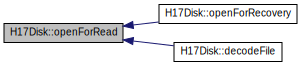
\includegraphics[width=350pt]{classH17Disk_a2d9e6faca3284d426af174b18554d4a9_icgraph}
\end{center}
\end{figure}


\hypertarget{classH17Disk_aa375761378f8a80cb8c5e479008c0e32}{}\index{H17\+Disk@{H17\+Disk}!open\+For\+Recovery@{open\+For\+Recovery}}
\index{open\+For\+Recovery@{open\+For\+Recovery}!H17\+Disk@{H17\+Disk}}
\subsubsection[{open\+For\+Recovery}]{\setlength{\rightskip}{0pt plus 5cm}bool H17\+Disk\+::open\+For\+Recovery (
\begin{DoxyParamCaption}
\item[{char $\ast$}]{name}
\end{DoxyParamCaption}
)\hspace{0.3cm}{\ttfamily [virtual]}}\label{classH17Disk_aa375761378f8a80cb8c5e479008c0e32}
open for recovery

Not yet implemented


\begin{DoxyParams}{Parameters}
{\em name} & file name\\
\hline
\end{DoxyParams}
\begin{DoxyReturn}{Returns}
success 
\end{DoxyReturn}


Definition at line 129 of file h17disk.\+cpp.



Here is the call graph for this function\+:
\nopagebreak
\begin{figure}[H]
\begin{center}
\leavevmode
\includegraphics[width=350pt]{classH17Disk_aa375761378f8a80cb8c5e479008c0e32_cgraph}
\end{center}
\end{figure}


\hypertarget{classH17Disk_ad29344c720e1a09c4de310d51ce40449}{}\index{H17\+Disk@{H17\+Disk}!open\+For\+Write@{open\+For\+Write}}
\index{open\+For\+Write@{open\+For\+Write}!H17\+Disk@{H17\+Disk}}
\subsubsection[{open\+For\+Write}]{\setlength{\rightskip}{0pt plus 5cm}bool H17\+Disk\+::open\+For\+Write (
\begin{DoxyParamCaption}
\item[{char $\ast$}]{name}
\end{DoxyParamCaption}
)\hspace{0.3cm}{\ttfamily [virtual]}}\label{classH17Disk_ad29344c720e1a09c4de310d51ce40449}
open file for writing


\begin{DoxyParams}{Parameters}
{\em name} & file name\\
\hline
\end{DoxyParams}
\begin{DoxyReturn}{Returns}
success 
\end{DoxyReturn}


Definition at line 85 of file h17disk.\+cpp.



Here is the caller graph for this function\+:
\nopagebreak
\begin{figure}[H]
\begin{center}
\leavevmode
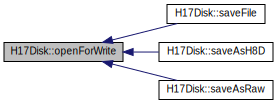
\includegraphics[width=349pt]{classH17Disk_ad29344c720e1a09c4de310d51ce40449_icgraph}
\end{center}
\end{figure}


\hypertarget{classH17Disk_a92edc41852a329daed3e91f50e0271c7}{}\index{H17\+Disk@{H17\+Disk}!save\+As\+H8\+D@{save\+As\+H8\+D}}
\index{save\+As\+H8\+D@{save\+As\+H8\+D}!H17\+Disk@{H17\+Disk}}
\subsubsection[{save\+As\+H8\+D}]{\setlength{\rightskip}{0pt plus 5cm}bool H17\+Disk\+::save\+As\+H8\+D (
\begin{DoxyParamCaption}
\item[{char $\ast$}]{name}
\end{DoxyParamCaption}
)\hspace{0.3cm}{\ttfamily [virtual]}}\label{classH17Disk_a92edc41852a329daed3e91f50e0271c7}
save h17disk image as a H8\+D file


\begin{DoxyParams}{Parameters}
{\em name} & H8\+D file name\\
\hline
\end{DoxyParams}
\begin{DoxyReturn}{Returns}
success 
\end{DoxyReturn}


Definition at line 214 of file h17disk.\+cpp.



Here is the call graph for this function\+:
\nopagebreak
\begin{figure}[H]
\begin{center}
\leavevmode
\includegraphics[width=349pt]{classH17Disk_a92edc41852a329daed3e91f50e0271c7_cgraph}
\end{center}
\end{figure}


\hypertarget{classH17Disk_a0a7412197ca1478393a45885cc132916}{}\index{H17\+Disk@{H17\+Disk}!save\+As\+Raw@{save\+As\+Raw}}
\index{save\+As\+Raw@{save\+As\+Raw}!H17\+Disk@{H17\+Disk}}
\subsubsection[{save\+As\+Raw}]{\setlength{\rightskip}{0pt plus 5cm}bool H17\+Disk\+::save\+As\+Raw (
\begin{DoxyParamCaption}
\item[{char $\ast$}]{name}
\end{DoxyParamCaption}
)\hspace{0.3cm}{\ttfamily [virtual]}}\label{classH17Disk_a0a7412197ca1478393a45885cc132916}
save h17disk image as a raw file


\begin{DoxyParams}{Parameters}
{\em name} & raw file name\\
\hline
\end{DoxyParams}
\begin{DoxyReturn}{Returns}
success 
\end{DoxyReturn}


Definition at line 242 of file h17disk.\+cpp.



Here is the call graph for this function\+:
\nopagebreak
\begin{figure}[H]
\begin{center}
\leavevmode
\includegraphics[width=349pt]{classH17Disk_a0a7412197ca1478393a45885cc132916_cgraph}
\end{center}
\end{figure}


\hypertarget{classH17Disk_adfb88c5c9f3c67a0923a4d24e5efe791}{}\index{H17\+Disk@{H17\+Disk}!save\+File@{save\+File}}
\index{save\+File@{save\+File}!H17\+Disk@{H17\+Disk}}
\subsubsection[{save\+File}]{\setlength{\rightskip}{0pt plus 5cm}bool H17\+Disk\+::save\+File (
\begin{DoxyParamCaption}
\item[{char $\ast$}]{name}
\end{DoxyParamCaption}
)\hspace{0.3cm}{\ttfamily [virtual]}}\label{classH17Disk_adfb88c5c9f3c67a0923a4d24e5efe791}
save file


\begin{DoxyParams}{Parameters}
{\em name} & file name\\
\hline
\end{DoxyParams}
\begin{DoxyReturn}{Returns}
success 
\end{DoxyReturn}


Definition at line 185 of file h17disk.\+cpp.



Here is the call graph for this function\+:
\nopagebreak
\begin{figure}[H]
\begin{center}
\leavevmode
\includegraphics[width=350pt]{classH17Disk_adfb88c5c9f3c67a0923a4d24e5efe791_cgraph}
\end{center}
\end{figure}


\hypertarget{classH17Disk_ad8755a4e016bea07fd30796d7b6c1ca0}{}\index{H17\+Disk@{H17\+Disk}!set\+Default\+Disk\+Format@{set\+Default\+Disk\+Format}}
\index{set\+Default\+Disk\+Format@{set\+Default\+Disk\+Format}!H17\+Disk@{H17\+Disk}}
\subsubsection[{set\+Default\+Disk\+Format}]{\setlength{\rightskip}{0pt plus 5cm}bool H17\+Disk\+::set\+Default\+Disk\+Format (
\begin{DoxyParamCaption}
{}
\end{DoxyParamCaption}
)\hspace{0.3cm}{\ttfamily [private]}, {\ttfamily [virtual]}}\label{classH17Disk_ad8755a4e016bea07fd30796d7b6c1ca0}
set default disk parameters

\begin{DoxyReturn}{Returns}
success 
\end{DoxyReturn}


Definition at line 2241 of file h17disk.\+cpp.



Here is the caller graph for this function\+:
\nopagebreak
\begin{figure}[H]
\begin{center}
\leavevmode
\includegraphics[width=350pt]{classH17Disk_ad8755a4e016bea07fd30796d7b6c1ca0_icgraph}
\end{center}
\end{figure}


\hypertarget{classH17Disk_a78bd33233d9597f81e69db936efe5356}{}\index{H17\+Disk@{H17\+Disk}!set\+Default\+Flags@{set\+Default\+Flags}}
\index{set\+Default\+Flags@{set\+Default\+Flags}!H17\+Disk@{H17\+Disk}}
\subsubsection[{set\+Default\+Flags}]{\setlength{\rightskip}{0pt plus 5cm}bool H17\+Disk\+::set\+Default\+Flags (
\begin{DoxyParamCaption}
{}
\end{DoxyParamCaption}
)\hspace{0.3cm}{\ttfamily [private]}, {\ttfamily [virtual]}}\label{classH17Disk_a78bd33233d9597f81e69db936efe5356}
set default flags

\begin{DoxyReturn}{Returns}
success 
\end{DoxyReturn}


Definition at line 2255 of file h17disk.\+cpp.



Here is the caller graph for this function\+:
\nopagebreak
\begin{figure}[H]
\begin{center}
\leavevmode
\includegraphics[width=350pt]{classH17Disk_a78bd33233d9597f81e69db936efe5356_icgraph}
\end{center}
\end{figure}


\hypertarget{classH17Disk_a6317e8bd90eed1f3785bcde079c72ae6}{}\index{H17\+Disk@{H17\+Disk}!set\+Defaults@{set\+Defaults}}
\index{set\+Defaults@{set\+Defaults}!H17\+Disk@{H17\+Disk}}
\subsubsection[{set\+Defaults}]{\setlength{\rightskip}{0pt plus 5cm}bool H17\+Disk\+::set\+Defaults (
\begin{DoxyParamCaption}
{}
\end{DoxyParamCaption}
)\hspace{0.3cm}{\ttfamily [private]}, {\ttfamily [virtual]}}\label{classH17Disk_a6317e8bd90eed1f3785bcde079c72ae6}
set default values for a h17disk file format

\begin{DoxyReturn}{Returns}
success 
\end{DoxyReturn}


Definition at line 2218 of file h17disk.\+cpp.



Here is the call graph for this function\+:
\nopagebreak
\begin{figure}[H]
\begin{center}
\leavevmode
\includegraphics[width=350pt]{classH17Disk_a6317e8bd90eed1f3785bcde079c72ae6_cgraph}
\end{center}
\end{figure}




Here is the caller graph for this function\+:
\nopagebreak
\begin{figure}[H]
\begin{center}
\leavevmode
\includegraphics[width=350pt]{classH17Disk_a6317e8bd90eed1f3785bcde079c72ae6_icgraph}
\end{center}
\end{figure}


\hypertarget{classH17Disk_a9aaab4accbcfce3205c0eadc9679a9f9}{}\index{H17\+Disk@{H17\+Disk}!set\+Distribution\+Parameter@{set\+Distribution\+Parameter}}
\index{set\+Distribution\+Parameter@{set\+Distribution\+Parameter}!H17\+Disk@{H17\+Disk}}
\subsubsection[{set\+Distribution\+Parameter}]{\setlength{\rightskip}{0pt plus 5cm}bool H17\+Disk\+::set\+Distribution\+Parameter (
\begin{DoxyParamCaption}
\item[{unsigned char}]{val}
\end{DoxyParamCaption}
)\hspace{0.3cm}{\ttfamily [virtual]}}\label{classH17Disk_a9aaab4accbcfce3205c0eadc9679a9f9}
set distribution parameter


\begin{DoxyParams}{Parameters}
{\em val} & \\
\hline
\end{DoxyParams}
\begin{DoxyReturn}{Returns}
success 
\end{DoxyReturn}


Definition at line 1714 of file h17disk.\+cpp.

\hypertarget{classH17Disk_a40df944449f21c6f5319024f0e179f7c}{}\index{H17\+Disk@{H17\+Disk}!set\+Sides@{set\+Sides}}
\index{set\+Sides@{set\+Sides}!H17\+Disk@{H17\+Disk}}
\subsubsection[{set\+Sides}]{\setlength{\rightskip}{0pt plus 5cm}bool H17\+Disk\+::set\+Sides (
\begin{DoxyParamCaption}
\item[{unsigned char}]{sides}
\end{DoxyParamCaption}
)\hspace{0.3cm}{\ttfamily [virtual]}}\label{classH17Disk_a40df944449f21c6f5319024f0e179f7c}
set the number of sides


\begin{DoxyParams}{Parameters}
{\em sides} & \\
\hline
\end{DoxyParams}
\begin{DoxyReturn}{Returns}
success 
\end{DoxyReturn}


Definition at line 1658 of file h17disk.\+cpp.

\hypertarget{classH17Disk_adda59abe2fa07a5b565f061346e1439a}{}\index{H17\+Disk@{H17\+Disk}!set\+Track\+Data\+Parameter@{set\+Track\+Data\+Parameter}}
\index{set\+Track\+Data\+Parameter@{set\+Track\+Data\+Parameter}!H17\+Disk@{H17\+Disk}}
\subsubsection[{set\+Track\+Data\+Parameter}]{\setlength{\rightskip}{0pt plus 5cm}bool H17\+Disk\+::set\+Track\+Data\+Parameter (
\begin{DoxyParamCaption}
\item[{unsigned char}]{val}
\end{DoxyParamCaption}
)\hspace{0.3cm}{\ttfamily [virtual]}}\label{classH17Disk_adda59abe2fa07a5b565f061346e1439a}
set track data parameter


\begin{DoxyParams}{Parameters}
{\em val} & \\
\hline
\end{DoxyParams}
\begin{DoxyReturn}{Returns}
success 
\end{DoxyReturn}


Definition at line 1728 of file h17disk.\+cpp.

\hypertarget{classH17Disk_a2e492914d9f408f25f1223253d20f5bc}{}\index{H17\+Disk@{H17\+Disk}!set\+Tracks@{set\+Tracks}}
\index{set\+Tracks@{set\+Tracks}!H17\+Disk@{H17\+Disk}}
\subsubsection[{set\+Tracks}]{\setlength{\rightskip}{0pt plus 5cm}bool H17\+Disk\+::set\+Tracks (
\begin{DoxyParamCaption}
\item[{unsigned char}]{tracks}
\end{DoxyParamCaption}
)\hspace{0.3cm}{\ttfamily [virtual]}}\label{classH17Disk_a2e492914d9f408f25f1223253d20f5bc}
set the number of tracks for the disk


\begin{DoxyParams}{Parameters}
{\em tracks} & \\
\hline
\end{DoxyParams}
\begin{DoxyReturn}{Returns}
success 
\end{DoxyReturn}


Definition at line 1672 of file h17disk.\+cpp.

\hypertarget{classH17Disk_aeedd102e18abe2cdcf8630d3cdc5492e}{}\index{H17\+Disk@{H17\+Disk}!set\+W\+P\+Parameter@{set\+W\+P\+Parameter}}
\index{set\+W\+P\+Parameter@{set\+W\+P\+Parameter}!H17\+Disk@{H17\+Disk}}
\subsubsection[{set\+W\+P\+Parameter}]{\setlength{\rightskip}{0pt plus 5cm}bool H17\+Disk\+::set\+W\+P\+Parameter (
\begin{DoxyParamCaption}
\item[{bool}]{val}
\end{DoxyParamCaption}
)\hspace{0.3cm}{\ttfamily [virtual]}}\label{classH17Disk_aeedd102e18abe2cdcf8630d3cdc5492e}
set write-\/protect for disk


\begin{DoxyParams}{Parameters}
{\em val} & \\
\hline
\end{DoxyParams}
\begin{DoxyReturn}{Returns}
success 
\end{DoxyReturn}


Definition at line 1700 of file h17disk.\+cpp.

\hypertarget{classH17Disk_ae95a1ef9181111102784f12dc00e341b}{}\index{H17\+Disk@{H17\+Disk}!start\+Data@{start\+Data}}
\index{start\+Data@{start\+Data}!H17\+Disk@{H17\+Disk}}
\subsubsection[{start\+Data}]{\setlength{\rightskip}{0pt plus 5cm}bool H17\+Disk\+::start\+Data (
\begin{DoxyParamCaption}
{}
\end{DoxyParamCaption}
)\hspace{0.3cm}{\ttfamily [virtual]}}\label{classH17Disk_ae95a1ef9181111102784f12dc00e341b}
start data block

\begin{DoxyReturn}{Returns}
success 
\end{DoxyReturn}


Definition at line 1904 of file h17disk.\+cpp.



Here is the call graph for this function\+:
\nopagebreak
\begin{figure}[H]
\begin{center}
\leavevmode
\includegraphics[width=350pt]{classH17Disk_ae95a1ef9181111102784f12dc00e341b_cgraph}
\end{center}
\end{figure}


\hypertarget{classH17Disk_a0eecc11273d8051ccb68b6975fa55fba}{}\index{H17\+Disk@{H17\+Disk}!start\+Track@{start\+Track}}
\index{start\+Track@{start\+Track}!H17\+Disk@{H17\+Disk}}
\subsubsection[{start\+Track}]{\setlength{\rightskip}{0pt plus 5cm}bool H17\+Disk\+::start\+Track (
\begin{DoxyParamCaption}
\item[{unsigned char}]{side, }
\item[{unsigned char}]{track}
\end{DoxyParamCaption}
)\hspace{0.3cm}{\ttfamily [virtual]}}\label{classH17Disk_a0eecc11273d8051ccb68b6975fa55fba}
start track for data.


\begin{DoxyParams}{Parameters}
{\em side} & \\
\hline
{\em track} & \\
\hline
\end{DoxyParams}
\begin{DoxyReturn}{Returns}
success 
\end{DoxyReturn}


Definition at line 1927 of file h17disk.\+cpp.

\hypertarget{classH17Disk_a29f4d35fba24f0d9cee37bcb02120a6c}{}\index{H17\+Disk@{H17\+Disk}!validate\+Block@{validate\+Block}}
\index{validate\+Block@{validate\+Block}!H17\+Disk@{H17\+Disk}}
\subsubsection[{validate\+Block}]{\setlength{\rightskip}{0pt plus 5cm}bool H17\+Disk\+::validate\+Block (
\begin{DoxyParamCaption}
\item[{unsigned char}]{buf\mbox{[}$\,$\mbox{]}, }
\item[{unsigned int}]{size, }
\item[{unsigned int \&}]{length}
\end{DoxyParamCaption}
)\hspace{0.3cm}{\ttfamily [virtual]}}\label{classH17Disk_a29f4d35fba24f0d9cee37bcb02120a6c}
validate block


\begin{DoxyParams}{Parameters}
{\em buf} & data buffer \\
\hline
{\em size} & size of buffer \\
\hline
{\em } & \\
\hline
\end{DoxyParams}
\begin{DoxyRefDesc}{Todo}
\item[\hyperlink{todo__todo000009}{Todo}]check to see if mandatory , and skip the data. \end{DoxyRefDesc}


Definition at line 490 of file h17disk.\+cpp.



Here is the call graph for this function\+:
\nopagebreak
\begin{figure}[H]
\begin{center}
\leavevmode
\includegraphics[width=350pt]{classH17Disk_a29f4d35fba24f0d9cee37bcb02120a6c_cgraph}
\end{center}
\end{figure}




Here is the caller graph for this function\+:
\nopagebreak
\begin{figure}[H]
\begin{center}
\leavevmode
\includegraphics[width=350pt]{classH17Disk_a29f4d35fba24f0d9cee37bcb02120a6c_icgraph}
\end{center}
\end{figure}


\hypertarget{classH17Disk_a0f8be0fb5d8f55eb6843b6668f60facd}{}\index{H17\+Disk@{H17\+Disk}!validate\+Comment\+Block@{validate\+Comment\+Block}}
\index{validate\+Comment\+Block@{validate\+Comment\+Block}!H17\+Disk@{H17\+Disk}}
\subsubsection[{validate\+Comment\+Block}]{\setlength{\rightskip}{0pt plus 5cm}bool H17\+Disk\+::validate\+Comment\+Block (
\begin{DoxyParamCaption}
\item[{unsigned char}]{buf\mbox{[}$\,$\mbox{]}, }
\item[{unsigned int}]{size}
\end{DoxyParamCaption}
)\hspace{0.3cm}{\ttfamily [virtual]}}\label{classH17Disk_a0f8be0fb5d8f55eb6843b6668f60facd}
validate Comment\+Block


\begin{DoxyParams}{Parameters}
{\em buf} & data buffer \\
\hline
{\em size} & size of buffer\\
\hline
\end{DoxyParams}
\begin{DoxyReturn}{Returns}
if load was successful 
\end{DoxyReturn}


Definition at line 738 of file h17disk.\+cpp.



Here is the caller graph for this function\+:
\nopagebreak
\begin{figure}[H]
\begin{center}
\leavevmode
\includegraphics[width=350pt]{classH17Disk_a0f8be0fb5d8f55eb6843b6668f60facd_icgraph}
\end{center}
\end{figure}


\hypertarget{classH17Disk_a593434e6ce0538943cb044b7d0c9c273}{}\index{H17\+Disk@{H17\+Disk}!validate\+Data\+Block@{validate\+Data\+Block}}
\index{validate\+Data\+Block@{validate\+Data\+Block}!H17\+Disk@{H17\+Disk}}
\subsubsection[{validate\+Data\+Block}]{\setlength{\rightskip}{0pt plus 5cm}bool H17\+Disk\+::validate\+Data\+Block (
\begin{DoxyParamCaption}
\item[{unsigned char}]{buf\mbox{[}$\,$\mbox{]}, }
\item[{unsigned int}]{size}
\end{DoxyParamCaption}
)\hspace{0.3cm}{\ttfamily [virtual]}}\label{classH17Disk_a593434e6ce0538943cb044b7d0c9c273}
validate Data\+Block


\begin{DoxyParams}{Parameters}
{\em buf} & data buffer \\
\hline
{\em size} & size of buffer\\
\hline
\end{DoxyParams}
\begin{DoxyReturn}{Returns}
if load was successful 
\end{DoxyReturn}


Definition at line 997 of file h17disk.\+cpp.



Here is the call graph for this function\+:
\nopagebreak
\begin{figure}[H]
\begin{center}
\leavevmode
\includegraphics[width=350pt]{classH17Disk_a593434e6ce0538943cb044b7d0c9c273_cgraph}
\end{center}
\end{figure}




Here is the caller graph for this function\+:
\nopagebreak
\begin{figure}[H]
\begin{center}
\leavevmode
\includegraphics[width=350pt]{classH17Disk_a593434e6ce0538943cb044b7d0c9c273_icgraph}
\end{center}
\end{figure}


\hypertarget{classH17Disk_a08c7c7f0cad0cc24224fc73227b9648e}{}\index{H17\+Disk@{H17\+Disk}!validate\+Date\+Block@{validate\+Date\+Block}}
\index{validate\+Date\+Block@{validate\+Date\+Block}!H17\+Disk@{H17\+Disk}}
\subsubsection[{validate\+Date\+Block}]{\setlength{\rightskip}{0pt plus 5cm}bool H17\+Disk\+::validate\+Date\+Block (
\begin{DoxyParamCaption}
\item[{unsigned char}]{buf\mbox{[}$\,$\mbox{]}, }
\item[{unsigned int}]{size}
\end{DoxyParamCaption}
)\hspace{0.3cm}{\ttfamily [virtual]}}\label{classH17Disk_a08c7c7f0cad0cc24224fc73227b9648e}
validate Date\+Block


\begin{DoxyParams}{Parameters}
{\em buf} & data buffer \\
\hline
{\em size} & size of buffer\\
\hline
\end{DoxyParams}
\begin{DoxyReturn}{Returns}
if load was successful 
\end{DoxyReturn}


Definition at line 788 of file h17disk.\+cpp.



Here is the caller graph for this function\+:
\nopagebreak
\begin{figure}[H]
\begin{center}
\leavevmode
\includegraphics[width=350pt]{classH17Disk_a08c7c7f0cad0cc24224fc73227b9648e_icgraph}
\end{center}
\end{figure}


\hypertarget{classH17Disk_aaf268125dfe0bb84c288aff63f5e865d}{}\index{H17\+Disk@{H17\+Disk}!validate\+Disk\+Format\+Block@{validate\+Disk\+Format\+Block}}
\index{validate\+Disk\+Format\+Block@{validate\+Disk\+Format\+Block}!H17\+Disk@{H17\+Disk}}
\subsubsection[{validate\+Disk\+Format\+Block}]{\setlength{\rightskip}{0pt plus 5cm}bool H17\+Disk\+::validate\+Disk\+Format\+Block (
\begin{DoxyParamCaption}
\item[{unsigned char}]{buf\mbox{[}$\,$\mbox{]}, }
\item[{unsigned int}]{size}
\end{DoxyParamCaption}
)\hspace{0.3cm}{\ttfamily [virtual]}}\label{classH17Disk_aaf268125dfe0bb84c288aff63f5e865d}
validate Disk\+Format\+Block


\begin{DoxyParams}{Parameters}
{\em buf} & data buffer \\
\hline
{\em size} & size of buffer\\
\hline
\end{DoxyParams}
\begin{DoxyReturn}{Returns}
if validation was succesful 
\end{DoxyReturn}


Definition at line 631 of file h17disk.\+cpp.



Here is the caller graph for this function\+:
\nopagebreak
\begin{figure}[H]
\begin{center}
\leavevmode
\includegraphics[width=350pt]{classH17Disk_aaf268125dfe0bb84c288aff63f5e865d_icgraph}
\end{center}
\end{figure}


\hypertarget{classH17Disk_a676a126b40c2697cbdeb32648a69c15d}{}\index{H17\+Disk@{H17\+Disk}!validate\+Flags\+Block@{validate\+Flags\+Block}}
\index{validate\+Flags\+Block@{validate\+Flags\+Block}!H17\+Disk@{H17\+Disk}}
\subsubsection[{validate\+Flags\+Block}]{\setlength{\rightskip}{0pt plus 5cm}bool H17\+Disk\+::validate\+Flags\+Block (
\begin{DoxyParamCaption}
\item[{unsigned char}]{buf\mbox{[}$\,$\mbox{]}, }
\item[{unsigned int}]{size}
\end{DoxyParamCaption}
)\hspace{0.3cm}{\ttfamily [virtual]}}\label{classH17Disk_a676a126b40c2697cbdeb32648a69c15d}
validate Flags\+Block


\begin{DoxyParams}{Parameters}
{\em buf} & data buffer \\
\hline
{\em size} & size of buffer\\
\hline
\end{DoxyParams}
\begin{DoxyReturn}{Returns}
if validation was successful 
\end{DoxyReturn}


Definition at line 936 of file h17disk.\+cpp.



Here is the caller graph for this function\+:
\nopagebreak
\begin{figure}[H]
\begin{center}
\leavevmode
\includegraphics[width=350pt]{classH17Disk_a676a126b40c2697cbdeb32648a69c15d_icgraph}
\end{center}
\end{figure}


\hypertarget{classH17Disk_ad9402e7823ac0a2741dc316cae361ecd}{}\index{H17\+Disk@{H17\+Disk}!validate\+Header@{validate\+Header}}
\index{validate\+Header@{validate\+Header}!H17\+Disk@{H17\+Disk}}
\subsubsection[{validate\+Header}]{\setlength{\rightskip}{0pt plus 5cm}bool H17\+Disk\+::validate\+Header (
\begin{DoxyParamCaption}
\item[{unsigned char}]{buf\mbox{[}$\,$\mbox{]}, }
\item[{unsigned int}]{size, }
\item[{unsigned int \&}]{length}
\end{DoxyParamCaption}
)\hspace{0.3cm}{\ttfamily [virtual]}}\label{classH17Disk_ad9402e7823ac0a2741dc316cae361ecd}
validate header of a h17disk file.


\begin{DoxyParams}{Parameters}
{\em buf} & data buffer \\
\hline
{\em size} & size of buffer \\
\hline
{\em } & \\
\hline
\end{DoxyParams}


Definition at line 419 of file h17disk.\+cpp.



Here is the caller graph for this function\+:
\nopagebreak
\begin{figure}[H]
\begin{center}
\leavevmode
\includegraphics[width=350pt]{classH17Disk_ad9402e7823ac0a2741dc316cae361ecd_icgraph}
\end{center}
\end{figure}


\hypertarget{classH17Disk_a592a6390ad6a382cae246886993954a7}{}\index{H17\+Disk@{H17\+Disk}!validate\+Imager\+Block@{validate\+Imager\+Block}}
\index{validate\+Imager\+Block@{validate\+Imager\+Block}!H17\+Disk@{H17\+Disk}}
\subsubsection[{validate\+Imager\+Block}]{\setlength{\rightskip}{0pt plus 5cm}bool H17\+Disk\+::validate\+Imager\+Block (
\begin{DoxyParamCaption}
\item[{unsigned char}]{buf\mbox{[}$\,$\mbox{]}, }
\item[{unsigned int}]{size}
\end{DoxyParamCaption}
)\hspace{0.3cm}{\ttfamily [virtual]}}\label{classH17Disk_a592a6390ad6a382cae246886993954a7}
validate Imager\+Block


\begin{DoxyParams}{Parameters}
{\em buf} & data buffer \\
\hline
{\em size} & size of buffer\\
\hline
\end{DoxyParams}
\begin{DoxyReturn}{Returns}
if load was successful 
\end{DoxyReturn}


Definition at line 837 of file h17disk.\+cpp.



Here is the caller graph for this function\+:
\nopagebreak
\begin{figure}[H]
\begin{center}
\leavevmode
\includegraphics[width=350pt]{classH17Disk_a592a6390ad6a382cae246886993954a7_icgraph}
\end{center}
\end{figure}


\hypertarget{classH17Disk_a80cc18809c189366f4c8ecf494286129}{}\index{H17\+Disk@{H17\+Disk}!validate\+Label\+Block@{validate\+Label\+Block}}
\index{validate\+Label\+Block@{validate\+Label\+Block}!H17\+Disk@{H17\+Disk}}
\subsubsection[{validate\+Label\+Block}]{\setlength{\rightskip}{0pt plus 5cm}bool H17\+Disk\+::validate\+Label\+Block (
\begin{DoxyParamCaption}
\item[{unsigned char}]{buf\mbox{[}$\,$\mbox{]}, }
\item[{unsigned int}]{size}
\end{DoxyParamCaption}
)\hspace{0.3cm}{\ttfamily [virtual]}}\label{classH17Disk_a80cc18809c189366f4c8ecf494286129}
validate Label\+Block


\begin{DoxyParams}{Parameters}
{\em buf} & data buffer \\
\hline
{\em size} & size of buffer\\
\hline
\end{DoxyParams}
\begin{DoxyReturn}{Returns}
if validation was succesful 
\end{DoxyReturn}


Definition at line 688 of file h17disk.\+cpp.



Here is the caller graph for this function\+:
\nopagebreak
\begin{figure}[H]
\begin{center}
\leavevmode
\includegraphics[width=350pt]{classH17Disk_a80cc18809c189366f4c8ecf494286129_icgraph}
\end{center}
\end{figure}


\hypertarget{classH17Disk_adc15505d580fdb29e57c67293d5b3cda}{}\index{H17\+Disk@{H17\+Disk}!validate\+Program\+Block@{validate\+Program\+Block}}
\index{validate\+Program\+Block@{validate\+Program\+Block}!H17\+Disk@{H17\+Disk}}
\subsubsection[{validate\+Program\+Block}]{\setlength{\rightskip}{0pt plus 5cm}bool H17\+Disk\+::validate\+Program\+Block (
\begin{DoxyParamCaption}
\item[{unsigned char}]{buf\mbox{[}$\,$\mbox{]}, }
\item[{unsigned int}]{size}
\end{DoxyParamCaption}
)\hspace{0.3cm}{\ttfamily [virtual]}}\label{classH17Disk_adc15505d580fdb29e57c67293d5b3cda}
validate Program\+Block


\begin{DoxyParams}{Parameters}
{\em buf} & data buffer \\
\hline
{\em size} & size of buffer\\
\hline
\end{DoxyParams}
\begin{DoxyReturn}{Returns}
if validation was successful 
\end{DoxyReturn}


Definition at line 887 of file h17disk.\+cpp.



Here is the caller graph for this function\+:
\nopagebreak
\begin{figure}[H]
\begin{center}
\leavevmode
\includegraphics[width=350pt]{classH17Disk_adc15505d580fdb29e57c67293d5b3cda_icgraph}
\end{center}
\end{figure}


\hypertarget{classH17Disk_ae1f57f11daa4d4c624d255851838d704}{}\index{H17\+Disk@{H17\+Disk}!validate\+Raw\+Data\+Block@{validate\+Raw\+Data\+Block}}
\index{validate\+Raw\+Data\+Block@{validate\+Raw\+Data\+Block}!H17\+Disk@{H17\+Disk}}
\subsubsection[{validate\+Raw\+Data\+Block}]{\setlength{\rightskip}{0pt plus 5cm}bool H17\+Disk\+::validate\+Raw\+Data\+Block (
\begin{DoxyParamCaption}
\item[{unsigned char}]{buf\mbox{[}$\,$\mbox{]}, }
\item[{unsigned int}]{size}
\end{DoxyParamCaption}
)\hspace{0.3cm}{\ttfamily [virtual]}}\label{classH17Disk_ae1f57f11daa4d4c624d255851838d704}
validate Raw\+Data\+Block


\begin{DoxyParams}{Parameters}
{\em buf} & data buffer \\
\hline
{\em size} & size of buffer\\
\hline
\end{DoxyParams}
\begin{DoxyReturn}{Returns}
if load was successful 
\end{DoxyReturn}


Definition at line 1390 of file h17disk.\+cpp.



Here is the call graph for this function\+:
\nopagebreak
\begin{figure}[H]
\begin{center}
\leavevmode
\includegraphics[width=350pt]{classH17Disk_ae1f57f11daa4d4c624d255851838d704_cgraph}
\end{center}
\end{figure}




Here is the caller graph for this function\+:
\nopagebreak
\begin{figure}[H]
\begin{center}
\leavevmode
\includegraphics[width=350pt]{classH17Disk_ae1f57f11daa4d4c624d255851838d704_icgraph}
\end{center}
\end{figure}


\hypertarget{classH17Disk_a60b9074cacd5a89f4b8e8dfb37bccf08}{}\index{H17\+Disk@{H17\+Disk}!validate\+Raw\+Sector\+Block@{validate\+Raw\+Sector\+Block}}
\index{validate\+Raw\+Sector\+Block@{validate\+Raw\+Sector\+Block}!H17\+Disk@{H17\+Disk}}
\subsubsection[{validate\+Raw\+Sector\+Block}]{\setlength{\rightskip}{0pt plus 5cm}bool H17\+Disk\+::validate\+Raw\+Sector\+Block (
\begin{DoxyParamCaption}
\item[{unsigned char}]{buf\mbox{[}$\,$\mbox{]}, }
\item[{unsigned int}]{size, }
\item[{unsigned int \&}]{length}
\end{DoxyParamCaption}
)\hspace{0.3cm}{\ttfamily [virtual]}}\label{classH17Disk_a60b9074cacd5a89f4b8e8dfb37bccf08}
validate raw sector block


\begin{DoxyParams}{Parameters}
{\em buf} & \\
\hline
{\em size} & \\
\hline
{\em length} & \\
\hline
\end{DoxyParams}
\begin{DoxyReturn}{Returns}
success 
\end{DoxyReturn}


Definition at line 1546 of file h17disk.\+cpp.



Here is the call graph for this function\+:
\nopagebreak
\begin{figure}[H]
\begin{center}
\leavevmode
\includegraphics[width=350pt]{classH17Disk_a60b9074cacd5a89f4b8e8dfb37bccf08_cgraph}
\end{center}
\end{figure}




Here is the caller graph for this function\+:
\nopagebreak
\begin{figure}[H]
\begin{center}
\leavevmode
\includegraphics[width=350pt]{classH17Disk_a60b9074cacd5a89f4b8e8dfb37bccf08_icgraph}
\end{center}
\end{figure}


\hypertarget{classH17Disk_a8f0fa7dbd52e633a2faa267e453cc486}{}\index{H17\+Disk@{H17\+Disk}!validate\+Raw\+Track\+Block@{validate\+Raw\+Track\+Block}}
\index{validate\+Raw\+Track\+Block@{validate\+Raw\+Track\+Block}!H17\+Disk@{H17\+Disk}}
\subsubsection[{validate\+Raw\+Track\+Block}]{\setlength{\rightskip}{0pt plus 5cm}bool H17\+Disk\+::validate\+Raw\+Track\+Block (
\begin{DoxyParamCaption}
\item[{unsigned char}]{buf\mbox{[}$\,$\mbox{]}, }
\item[{unsigned int}]{size, }
\item[{unsigned int \&}]{length}
\end{DoxyParamCaption}
)\hspace{0.3cm}{\ttfamily [virtual]}}\label{classH17Disk_a8f0fa7dbd52e633a2faa267e453cc486}
validate Raw\+Track\+Block


\begin{DoxyParams}{Parameters}
{\em buf} & data buffer \\
\hline
{\em size} & size of buffer \\
\hline
{\em length} & length of buffer used\\
\hline
\end{DoxyParams}
\begin{DoxyReturn}{Returns}
if load was successful 
\end{DoxyReturn}


Definition at line 1453 of file h17disk.\+cpp.



Here is the call graph for this function\+:
\nopagebreak
\begin{figure}[H]
\begin{center}
\leavevmode
\includegraphics[width=350pt]{classH17Disk_a8f0fa7dbd52e633a2faa267e453cc486_cgraph}
\end{center}
\end{figure}




Here is the caller graph for this function\+:
\nopagebreak
\begin{figure}[H]
\begin{center}
\leavevmode
\includegraphics[width=350pt]{classH17Disk_a8f0fa7dbd52e633a2faa267e453cc486_icgraph}
\end{center}
\end{figure}


\hypertarget{classH17Disk_a11e3a3c52730f4502a61f69035d7ab38}{}\index{H17\+Disk@{H17\+Disk}!validate\+Sector\+Block@{validate\+Sector\+Block}}
\index{validate\+Sector\+Block@{validate\+Sector\+Block}!H17\+Disk@{H17\+Disk}}
\subsubsection[{validate\+Sector\+Block}]{\setlength{\rightskip}{0pt plus 5cm}bool H17\+Disk\+::validate\+Sector\+Block (
\begin{DoxyParamCaption}
\item[{unsigned char}]{buf\mbox{[}$\,$\mbox{]}, }
\item[{unsigned int}]{size, }
\item[{unsigned int \&}]{length}
\end{DoxyParamCaption}
)\hspace{0.3cm}{\ttfamily [virtual]}}\label{classH17Disk_a11e3a3c52730f4502a61f69035d7ab38}
validate Sector\+Block


\begin{DoxyParams}{Parameters}
{\em buf} & data buffer \\
\hline
{\em size} & size of buffer \\
\hline
{\em length} & bytes used in buffer for this block\\
\hline
\end{DoxyParams}
\begin{DoxyReturn}{Returns}
if load was successful 
\end{DoxyReturn}


Definition at line 1140 of file h17disk.\+cpp.



Here is the call graph for this function\+:
\nopagebreak
\begin{figure}[H]
\begin{center}
\leavevmode
\includegraphics[width=350pt]{classH17Disk_a11e3a3c52730f4502a61f69035d7ab38_cgraph}
\end{center}
\end{figure}




Here is the caller graph for this function\+:
\nopagebreak
\begin{figure}[H]
\begin{center}
\leavevmode
\includegraphics[width=350pt]{classH17Disk_a11e3a3c52730f4502a61f69035d7ab38_icgraph}
\end{center}
\end{figure}


\hypertarget{classH17Disk_a532c7c77626521afd001ed4a32610912}{}\index{H17\+Disk@{H17\+Disk}!validate\+Track\+Block@{validate\+Track\+Block}}
\index{validate\+Track\+Block@{validate\+Track\+Block}!H17\+Disk@{H17\+Disk}}
\subsubsection[{validate\+Track\+Block}]{\setlength{\rightskip}{0pt plus 5cm}bool H17\+Disk\+::validate\+Track\+Block (
\begin{DoxyParamCaption}
\item[{unsigned char}]{buf\mbox{[}$\,$\mbox{]}, }
\item[{unsigned int}]{size, }
\item[{unsigned int \&}]{length}
\end{DoxyParamCaption}
)\hspace{0.3cm}{\ttfamily [virtual]}}\label{classH17Disk_a532c7c77626521afd001ed4a32610912}
validate Track\+Block


\begin{DoxyParams}{Parameters}
{\em buf} & data buffer \\
\hline
{\em size} & size of buffer \\
\hline
{\em length} & bytes used in buffer for this block\\
\hline
\end{DoxyParams}
\begin{DoxyReturn}{Returns}
if load was successful 
\end{DoxyReturn}


Definition at line 1062 of file h17disk.\+cpp.



Here is the call graph for this function\+:
\nopagebreak
\begin{figure}[H]
\begin{center}
\leavevmode
\includegraphics[width=350pt]{classH17Disk_a532c7c77626521afd001ed4a32610912_cgraph}
\end{center}
\end{figure}




Here is the caller graph for this function\+:
\nopagebreak
\begin{figure}[H]
\begin{center}
\leavevmode
\includegraphics[width=350pt]{classH17Disk_a532c7c77626521afd001ed4a32610912_icgraph}
\end{center}
\end{figure}


\hypertarget{classH17Disk_a988a0510cf62884ebf3dc3fc9c43d0b8}{}\index{H17\+Disk@{H17\+Disk}!write\+Block\+Header@{write\+Block\+Header}}
\index{write\+Block\+Header@{write\+Block\+Header}!H17\+Disk@{H17\+Disk}}
\subsubsection[{write\+Block\+Header}]{\setlength{\rightskip}{0pt plus 5cm}bool H17\+Disk\+::write\+Block\+Header (
\begin{DoxyParamCaption}
\item[{uint8\+\_\+t}]{block\+Id, }
\item[{uint8\+\_\+t}]{flag, }
\item[{uint32\+\_\+t}]{length}
\end{DoxyParamCaption}
)\hspace{0.3cm}{\ttfamily [private]}}\label{classH17Disk_a988a0510cf62884ebf3dc3fc9c43d0b8}
Common code to write the block header


\begin{DoxyParams}{Parameters}
{\em block\+Id} & Block I\+D \\
\hline
{\em flag} & Flag Byte \\
\hline
{\em length} & length of block\\
\hline
\end{DoxyParams}
\begin{DoxyReturn}{Returns}
if successful 
\end{DoxyReturn}


Definition at line 1785 of file h17disk.\+cpp.



Here is the caller graph for this function\+:
\nopagebreak
\begin{figure}[H]
\begin{center}
\leavevmode
\includegraphics[width=350pt]{classH17Disk_a988a0510cf62884ebf3dc3fc9c43d0b8_icgraph}
\end{center}
\end{figure}


\hypertarget{classH17Disk_a00a11fce25f33fd27437ac32e5f6139a}{}\index{H17\+Disk@{H17\+Disk}!write\+Comment@{write\+Comment}}
\index{write\+Comment@{write\+Comment}!H17\+Disk@{H17\+Disk}}
\subsubsection[{write\+Comment}]{\setlength{\rightskip}{0pt plus 5cm}bool H17\+Disk\+::write\+Comment (
\begin{DoxyParamCaption}
\item[{unsigned char $\ast$}]{buf, }
\item[{uint32\+\_\+t}]{length}
\end{DoxyParamCaption}
)\hspace{0.3cm}{\ttfamily [virtual]}}\label{classH17Disk_a00a11fce25f33fd27437ac32e5f6139a}
write comment block


\begin{DoxyParams}{Parameters}
{\em buf} & \\
\hline
{\em length} & \\
\hline
\end{DoxyParams}
\begin{DoxyReturn}{Returns}
success 
\end{DoxyReturn}


Definition at line 1831 of file h17disk.\+cpp.



Here is the call graph for this function\+:
\nopagebreak
\begin{figure}[H]
\begin{center}
\leavevmode
\includegraphics[width=350pt]{classH17Disk_a00a11fce25f33fd27437ac32e5f6139a_cgraph}
\end{center}
\end{figure}


\hypertarget{classH17Disk_ab397651808bc9ffd033584cbe5c1a8be}{}\index{H17\+Disk@{H17\+Disk}!write\+Date@{write\+Date}}
\index{write\+Date@{write\+Date}!H17\+Disk@{H17\+Disk}}
\subsubsection[{write\+Date}]{\setlength{\rightskip}{0pt plus 5cm}bool H17\+Disk\+::write\+Date (
\begin{DoxyParamCaption}
\item[{unsigned char $\ast$}]{buf, }
\item[{uint32\+\_\+t}]{length}
\end{DoxyParamCaption}
)\hspace{0.3cm}{\ttfamily [virtual]}}\label{classH17Disk_ab397651808bc9ffd033584cbe5c1a8be}
write date block


\begin{DoxyParams}{Parameters}
{\em buf} & \\
\hline
{\em length} & \\
\hline
\end{DoxyParams}
\begin{DoxyReturn}{Returns}
success 
\end{DoxyReturn}


Definition at line 1850 of file h17disk.\+cpp.



Here is the call graph for this function\+:
\nopagebreak
\begin{figure}[H]
\begin{center}
\leavevmode
\includegraphics[width=350pt]{classH17Disk_ab397651808bc9ffd033584cbe5c1a8be_cgraph}
\end{center}
\end{figure}


\hypertarget{classH17Disk_a888f6eb9e66d45410eb80903df0133d3}{}\index{H17\+Disk@{H17\+Disk}!write\+Disk\+Format\+Block@{write\+Disk\+Format\+Block}}
\index{write\+Disk\+Format\+Block@{write\+Disk\+Format\+Block}!H17\+Disk@{H17\+Disk}}
\subsubsection[{write\+Disk\+Format\+Block}]{\setlength{\rightskip}{0pt plus 5cm}bool H17\+Disk\+::write\+Disk\+Format\+Block (
\begin{DoxyParamCaption}
{}
\end{DoxyParamCaption}
)\hspace{0.3cm}{\ttfamily [virtual]}}\label{classH17Disk_a888f6eb9e66d45410eb80903df0133d3}
write disk format block

\begin{DoxyReturn}{Returns}
success 
\end{DoxyReturn}


Definition at line 1684 of file h17disk.\+cpp.



Here is the call graph for this function\+:
\nopagebreak
\begin{figure}[H]
\begin{center}
\leavevmode
\includegraphics[width=350pt]{classH17Disk_a888f6eb9e66d45410eb80903df0133d3_cgraph}
\end{center}
\end{figure}


\hypertarget{classH17Disk_a8390bffa0553266decd2e1c21831ea5f}{}\index{H17\+Disk@{H17\+Disk}!write\+Header@{write\+Header}}
\index{write\+Header@{write\+Header}!H17\+Disk@{H17\+Disk}}
\subsubsection[{write\+Header}]{\setlength{\rightskip}{0pt plus 5cm}bool H17\+Disk\+::write\+Header (
\begin{DoxyParamCaption}
{}
\end{DoxyParamCaption}
)\hspace{0.3cm}{\ttfamily [virtual]}}\label{classH17Disk_a8390bffa0553266decd2e1c21831ea5f}
write File Header

\begin{DoxyReturn}{Returns}
success 
\end{DoxyReturn}


Definition at line 1633 of file h17disk.\+cpp.



Here is the caller graph for this function\+:
\nopagebreak
\begin{figure}[H]
\begin{center}
\leavevmode
\includegraphics[width=327pt]{classH17Disk_a8390bffa0553266decd2e1c21831ea5f_icgraph}
\end{center}
\end{figure}


\hypertarget{classH17Disk_abed5956f503f0cd51cdb8ebe6cb26c9d}{}\index{H17\+Disk@{H17\+Disk}!write\+Imager@{write\+Imager}}
\index{write\+Imager@{write\+Imager}!H17\+Disk@{H17\+Disk}}
\subsubsection[{write\+Imager}]{\setlength{\rightskip}{0pt plus 5cm}bool H17\+Disk\+::write\+Imager (
\begin{DoxyParamCaption}
\item[{unsigned char $\ast$}]{buf, }
\item[{uint32\+\_\+t}]{length}
\end{DoxyParamCaption}
)\hspace{0.3cm}{\ttfamily [virtual]}}\label{classH17Disk_abed5956f503f0cd51cdb8ebe6cb26c9d}
write imager block


\begin{DoxyParams}{Parameters}
{\em buf} & \\
\hline
{\em length} & \\
\hline
\end{DoxyParams}
\begin{DoxyReturn}{Returns}
success 
\end{DoxyReturn}


Definition at line 1869 of file h17disk.\+cpp.



Here is the call graph for this function\+:
\nopagebreak
\begin{figure}[H]
\begin{center}
\leavevmode
\includegraphics[width=350pt]{classH17Disk_abed5956f503f0cd51cdb8ebe6cb26c9d_cgraph}
\end{center}
\end{figure}


\hypertarget{classH17Disk_ac4229315d8704036fe339189cbb649cb}{}\index{H17\+Disk@{H17\+Disk}!write\+Label@{write\+Label}}
\index{write\+Label@{write\+Label}!H17\+Disk@{H17\+Disk}}
\subsubsection[{write\+Label}]{\setlength{\rightskip}{0pt plus 5cm}bool H17\+Disk\+::write\+Label (
\begin{DoxyParamCaption}
\item[{unsigned char $\ast$}]{buf, }
\item[{uint32\+\_\+t}]{length}
\end{DoxyParamCaption}
)\hspace{0.3cm}{\ttfamily [virtual]}}\label{classH17Disk_ac4229315d8704036fe339189cbb649cb}
write label block


\begin{DoxyParams}{Parameters}
{\em buf} & \\
\hline
{\em length} & \\
\hline
\end{DoxyParams}
\begin{DoxyReturn}{Returns}
success 
\end{DoxyReturn}


Definition at line 1812 of file h17disk.\+cpp.



Here is the call graph for this function\+:
\nopagebreak
\begin{figure}[H]
\begin{center}
\leavevmode
\includegraphics[width=350pt]{classH17Disk_ac4229315d8704036fe339189cbb649cb_cgraph}
\end{center}
\end{figure}


\hypertarget{classH17Disk_a678d8b2633be207d5e3879f41991bcf5}{}\index{H17\+Disk@{H17\+Disk}!write\+Parameters@{write\+Parameters}}
\index{write\+Parameters@{write\+Parameters}!H17\+Disk@{H17\+Disk}}
\subsubsection[{write\+Parameters}]{\setlength{\rightskip}{0pt plus 5cm}bool H17\+Disk\+::write\+Parameters (
\begin{DoxyParamCaption}
{}
\end{DoxyParamCaption}
)\hspace{0.3cm}{\ttfamily [virtual]}}\label{classH17Disk_a678d8b2633be207d5e3879f41991bcf5}
write parameter block

\begin{DoxyReturn}{Returns}
success 
\end{DoxyReturn}


Definition at line 1740 of file h17disk.\+cpp.



Here is the call graph for this function\+:
\nopagebreak
\begin{figure}[H]
\begin{center}
\leavevmode
\includegraphics[width=350pt]{classH17Disk_a678d8b2633be207d5e3879f41991bcf5_cgraph}
\end{center}
\end{figure}


\hypertarget{classH17Disk_a71da855358f9c45a027be13ae2009a5e}{}\index{H17\+Disk@{H17\+Disk}!write\+Program@{write\+Program}}
\index{write\+Program@{write\+Program}!H17\+Disk@{H17\+Disk}}
\subsubsection[{write\+Program}]{\setlength{\rightskip}{0pt plus 5cm}bool H17\+Disk\+::write\+Program (
\begin{DoxyParamCaption}
\item[{unsigned char $\ast$}]{buf, }
\item[{uint32\+\_\+t}]{length}
\end{DoxyParamCaption}
)\hspace{0.3cm}{\ttfamily [virtual]}}\label{classH17Disk_a71da855358f9c45a027be13ae2009a5e}
write program


\begin{DoxyParams}{Parameters}
{\em buf} & \\
\hline
{\em length} & \\
\hline
\end{DoxyParams}
\begin{DoxyReturn}{Returns}
success 
\end{DoxyReturn}


Definition at line 1888 of file h17disk.\+cpp.



Here is the call graph for this function\+:
\nopagebreak
\begin{figure}[H]
\begin{center}
\leavevmode
\includegraphics[width=350pt]{classH17Disk_a71da855358f9c45a027be13ae2009a5e_cgraph}
\end{center}
\end{figure}


\hypertarget{classH17Disk_a453aedc5aa6cb970c6e174eadb4c6479}{}\index{H17\+Disk@{H17\+Disk}!write\+Raw\+Data\+Block@{write\+Raw\+Data\+Block}}
\index{write\+Raw\+Data\+Block@{write\+Raw\+Data\+Block}!H17\+Disk@{H17\+Disk}}
\subsubsection[{write\+Raw\+Data\+Block}]{\setlength{\rightskip}{0pt plus 5cm}bool H17\+Disk\+::write\+Raw\+Data\+Block (
\begin{DoxyParamCaption}
{}
\end{DoxyParamCaption}
)\hspace{0.3cm}{\ttfamily [virtual]}}\label{classH17Disk_a453aedc5aa6cb970c6e174eadb4c6479}
write raw data block

\begin{DoxyReturn}{Returns}
success 
\end{DoxyReturn}


Definition at line 2074 of file h17disk.\+cpp.



The documentation for this class was generated from the following files\+:\begin{DoxyCompactItemize}
\item 
\hyperlink{h17disk_8h}{h17disk.\+h}\item 
\hyperlink{h17disk_8cpp}{h17disk.\+cpp}\end{DoxyCompactItemize}

\input{classH17DiskCommentBlock}
\hypertarget{classH17DiskDataBlock}{}\section{H17\+Disk\+Data\+Block Class Reference}
\label{classH17DiskDataBlock}\index{H17\+Disk\+Data\+Block@{H17\+Disk\+Data\+Block}}


Inheritance diagram for H17\+Disk\+Data\+Block\+:
\nopagebreak
\begin{figure}[H]
\begin{center}
\leavevmode
\includegraphics[width=181pt]{classH17DiskDataBlock__inherit__graph}
\end{center}
\end{figure}


Collaboration diagram for H17\+Disk\+Data\+Block\+:
\nopagebreak
\begin{figure}[H]
\begin{center}
\leavevmode
\includegraphics[width=272pt]{classH17DiskDataBlock__coll__graph}
\end{center}
\end{figure}
\subsection*{Public Member Functions}
\begin{DoxyCompactItemize}
\item 
\hypertarget{classH17DiskDataBlock_a539b4d785f3b4395d9f47cbc131130fa}{}{\bfseries H17\+Disk\+Data\+Block} (uint8\+\_\+t buf\mbox{[}$\,$\mbox{]}, uint32\+\_\+t size)\label{classH17DiskDataBlock_a539b4d785f3b4395d9f47cbc131130fa}

\item 
virtual uint8\+\_\+t \hyperlink{classH17DiskDataBlock_a944cae8a6ba7b97a668654f787b908be}{get\+Block\+Id} ()
\item 
virtual bool \hyperlink{classH17DiskDataBlock_a6d7181e767bbc590cfee7c589c56930a}{write\+To\+File} (std\+::ofstream \&file)
\item 
virtual bool \hyperlink{classH17DiskDataBlock_a7a3764e8bc657aaf14e22ab92b63286d}{get\+Mandatory} ()
\item 
virtual bool \hyperlink{classH17DiskDataBlock_a6a940fded933fb4817c7b2b9dc7cea71}{dump} (uint8\+\_\+t level)
\item 
virtual bool \hyperlink{classH17DiskDataBlock_af03dbc5721ae46852aa286866959e45c}{analyze} ()
\item 
\hypertarget{classH17DiskDataBlock_ab7b123e3dc0d676b742c3730f4705f7d}{}virtual void {\bfseries print\+Block\+Name} ()\label{classH17DiskDataBlock_ab7b123e3dc0d676b742c3730f4705f7d}

\item 
virtual bool \hyperlink{classH17DiskDataBlock_ae78e78ea9f088f377b6de4fbec38b966}{write\+As\+H8\+D} (std\+::ofstream \&file)
\item 
virtual bool \hyperlink{classH17DiskDataBlock_a07b43b2694f0d89847b701d9c17f22f9}{write\+As\+Raw} (std\+::ofstream \&file)
\item 
virtual uint32\+\_\+t \hyperlink{classH17Block_aa2e87b141623b4c897c5337ea0535d1c}{get\+Data\+Size} ()
\item 
virtual uint8\+\_\+t $\ast$ \hyperlink{classH17Block_a6c2432cccdacdfb1a335bd924f19d942}{get\+Data} ()
\item 
virtual uint32\+\_\+t \hyperlink{classH17Block_a0327b6359cdf502269bbb7c6f35fae18}{get\+Block\+Size} ()
\item 
virtual uint32\+\_\+t \hyperlink{classH17Block_ad71ae203afc8713d4ee7416757fadbbe}{get\+Header\+Size} ()
\item 
virtual bool \hyperlink{classH17Block_a5c4d56a6c991c87fb9215797ce63b804}{write\+Block\+Header} (std\+::ofstream \&file)
\end{DoxyCompactItemize}
\subsection*{Static Public Attributes}
\begin{DoxyCompactItemize}
\item 
\hypertarget{classH17Block_a2c0bb47f26439845bada4b36ad517a19}{}static const uint8\+\_\+t {\bfseries Disk\+Format\+Block\+\_\+c} = 0x00\label{classH17Block_a2c0bb47f26439845bada4b36ad517a19}

\item 
\hypertarget{classH17Block_a321d17f4fa4f0c3bae07903dc9d63e89}{}static const uint8\+\_\+t {\bfseries Flags\+Block\+\_\+c} = 0x01\label{classH17Block_a321d17f4fa4f0c3bae07903dc9d63e89}

\item 
\hypertarget{classH17Block_a665b016e0c21812300c78e27bd27cacc}{}static const uint8\+\_\+t {\bfseries Label\+Block\+\_\+c} = 0x02\label{classH17Block_a665b016e0c21812300c78e27bd27cacc}

\item 
\hypertarget{classH17Block_a7e113d95265854d65ee7cfd9b8036bb4}{}static const uint8\+\_\+t {\bfseries Comment\+Block\+\_\+c} = 0x03\label{classH17Block_a7e113d95265854d65ee7cfd9b8036bb4}

\item 
\hypertarget{classH17Block_a6533f08296fa7781ab424014c53d0339}{}static const uint8\+\_\+t {\bfseries Date\+Block\+\_\+c} = 0x04\label{classH17Block_a6533f08296fa7781ab424014c53d0339}

\item 
\hypertarget{classH17Block_a6d3c62d3bb52383b0d42c96a0edf084e}{}static const uint8\+\_\+t {\bfseries Imager\+Block\+\_\+c} = 0x05\label{classH17Block_a6d3c62d3bb52383b0d42c96a0edf084e}

\item 
\hypertarget{classH17Block_a82d84c0c8a48dd51d2aa81a2bb25b388}{}static const uint8\+\_\+t {\bfseries Program\+Block\+\_\+c} = 0x06\label{classH17Block_a82d84c0c8a48dd51d2aa81a2bb25b388}

\item 
\hypertarget{classH17Block_ae6f576b907f36413c246f4d0121f81a2}{}static const uint8\+\_\+t {\bfseries Data\+Block\+\_\+c} = 0x10\label{classH17Block_ae6f576b907f36413c246f4d0121f81a2}

\item 
\hypertarget{classH17Block_a40da95004bf44a8b227e58d273de483f}{}static const uint8\+\_\+t {\bfseries Raw\+Data\+Block\+\_\+c} = 0x30\label{classH17Block_a40da95004bf44a8b227e58d273de483f}

\item 
\hypertarget{classH17Block_abba04ea8a19a2c67c52b2044e9d7e6b5}{}static const uint8\+\_\+t {\bfseries Track\+Data\+Id} = 0x11\label{classH17Block_abba04ea8a19a2c67c52b2044e9d7e6b5}

\item 
\hypertarget{classH17Block_aba48bf0cd556e2450f6ae849dee5aa58}{}static const uint8\+\_\+t {\bfseries Sector\+Data\+Id} = 0x12\label{classH17Block_aba48bf0cd556e2450f6ae849dee5aa58}

\item 
\hypertarget{classH17Block_af851d13f0569ae7860ce8e5953bfa5f5}{}static const uint8\+\_\+t {\bfseries Raw\+Track\+Data\+Id} = 0x31\label{classH17Block_af851d13f0569ae7860ce8e5953bfa5f5}

\item 
\hypertarget{classH17Block_a0510af71536a81a626c9956302b744bf}{}static const uint8\+\_\+t {\bfseries Raw\+Sector\+Data\+Id} = 0x32\label{classH17Block_a0510af71536a81a626c9956302b744bf}

\end{DoxyCompactItemize}
\subsection*{Protected Member Functions}
\begin{DoxyCompactItemize}
\item 
virtual bool \hyperlink{classH17Block_a09d4bee92e3b1862412b53a369f9dcc8}{dump\+Text} ()
\end{DoxyCompactItemize}
\subsection*{Protected Attributes}
\begin{DoxyCompactItemize}
\item 
\hypertarget{classH17Block_af5613c8a2286e67b7f8235162453d8c1}{}uint32\+\_\+t {\bfseries size\+\_\+m}\label{classH17Block_af5613c8a2286e67b7f8235162453d8c1}

\item 
\hypertarget{classH17Block_a279340cf9f0dba5b047297e38d430bb1}{}uint8\+\_\+t $\ast$ {\bfseries buf\+\_\+m}\label{classH17Block_a279340cf9f0dba5b047297e38d430bb1}

\end{DoxyCompactItemize}
\subsection*{Static Protected Attributes}
\begin{DoxyCompactItemize}
\item 
\hypertarget{classH17Block_a12fca0c1752b9473f618bd35cac1844f}{}static const uint32\+\_\+t {\bfseries block\+Header\+Size\+\_\+c} = 6\label{classH17Block_a12fca0c1752b9473f618bd35cac1844f}

\end{DoxyCompactItemize}
\subsection*{Private Attributes}
\begin{DoxyCompactItemize}
\item 
\hypertarget{classH17DiskDataBlock_ad13d99e9b61c91cbe5140c7957833f4f}{}std\+::vector$<$ \hyperlink{classTrack}{Track} $\ast$ $>$ {\bfseries tracks\+\_\+m}\label{classH17DiskDataBlock_ad13d99e9b61c91cbe5140c7957833f4f}

\end{DoxyCompactItemize}


\subsection{Detailed Description}


Definition at line 200 of file h17block.\+h.



\subsection{Member Function Documentation}
\hypertarget{classH17DiskDataBlock_af03dbc5721ae46852aa286866959e45c}{}\index{H17\+Disk\+Data\+Block@{H17\+Disk\+Data\+Block}!analyze@{analyze}}
\index{analyze@{analyze}!H17\+Disk\+Data\+Block@{H17\+Disk\+Data\+Block}}
\subsubsection[{analyze}]{\setlength{\rightskip}{0pt plus 5cm}bool H17\+Disk\+Data\+Block\+::analyze (
\begin{DoxyParamCaption}
{}
\end{DoxyParamCaption}
)\hspace{0.3cm}{\ttfamily [virtual]}}\label{classH17DiskDataBlock_af03dbc5721ae46852aa286866959e45c}
analyze the tracks

\begin{DoxyReturn}{Returns}
success 
\end{DoxyReturn}


Reimplemented from \hyperlink{classH17Block}{H17\+Block}.



Definition at line 916 of file h17block.\+cpp.

\hypertarget{classH17DiskDataBlock_a6a940fded933fb4817c7b2b9dc7cea71}{}\index{H17\+Disk\+Data\+Block@{H17\+Disk\+Data\+Block}!dump@{dump}}
\index{dump@{dump}!H17\+Disk\+Data\+Block@{H17\+Disk\+Data\+Block}}
\subsubsection[{dump}]{\setlength{\rightskip}{0pt plus 5cm}bool H17\+Disk\+Data\+Block\+::dump (
\begin{DoxyParamCaption}
\item[{uint8\+\_\+t}]{level}
\end{DoxyParamCaption}
)\hspace{0.3cm}{\ttfamily [virtual]}}\label{classH17DiskDataBlock_a6a940fded933fb4817c7b2b9dc7cea71}
dump the block to stdout


\begin{DoxyParams}{Parameters}
{\em level} & -\/ detail level to display 0 -\/ none 1 -\/ minimal 2 -\/ some 3 -\/ lots 4 -\/ complete\\
\hline
\end{DoxyParams}
\begin{DoxyReturn}{Returns}
success 
\end{DoxyReturn}


Reimplemented from \hyperlink{classH17Block_ac17cf2a0e1699277192063e13bee30b1}{H17\+Block}.



Definition at line 904 of file h17block.\+cpp.

\hypertarget{classH17Block_a09d4bee92e3b1862412b53a369f9dcc8}{}\index{H17\+Disk\+Data\+Block@{H17\+Disk\+Data\+Block}!dump\+Text@{dump\+Text}}
\index{dump\+Text@{dump\+Text}!H17\+Disk\+Data\+Block@{H17\+Disk\+Data\+Block}}
\subsubsection[{dump\+Text}]{\setlength{\rightskip}{0pt plus 5cm}bool H17\+Block\+::dump\+Text (
\begin{DoxyParamCaption}
{}
\end{DoxyParamCaption}
)\hspace{0.3cm}{\ttfamily [protected]}, {\ttfamily [virtual]}, {\ttfamily [inherited]}}\label{classH17Block_a09d4bee92e3b1862412b53a369f9dcc8}
dump text

\begin{DoxyReturn}{Returns}
true 
\end{DoxyReturn}


Definition at line 168 of file h17block.\+cpp.



Here is the caller graph for this function\+:
\nopagebreak
\begin{figure}[H]
\begin{center}
\leavevmode
\includegraphics[width=350pt]{classH17Block_a09d4bee92e3b1862412b53a369f9dcc8_icgraph}
\end{center}
\end{figure}


\hypertarget{classH17DiskDataBlock_a944cae8a6ba7b97a668654f787b908be}{}\index{H17\+Disk\+Data\+Block@{H17\+Disk\+Data\+Block}!get\+Block\+Id@{get\+Block\+Id}}
\index{get\+Block\+Id@{get\+Block\+Id}!H17\+Disk\+Data\+Block@{H17\+Disk\+Data\+Block}}
\subsubsection[{get\+Block\+Id}]{\setlength{\rightskip}{0pt plus 5cm}uint8\+\_\+t H17\+Disk\+Data\+Block\+::get\+Block\+Id (
\begin{DoxyParamCaption}
{}
\end{DoxyParamCaption}
)\hspace{0.3cm}{\ttfamily [virtual]}}\label{classH17DiskDataBlock_a944cae8a6ba7b97a668654f787b908be}
get block id

\begin{DoxyReturn}{Returns}
block id 
\end{DoxyReturn}


Implements \hyperlink{classH17Block}{H17\+Block}.



Definition at line 827 of file h17block.\+cpp.

\hypertarget{classH17Block_a0327b6359cdf502269bbb7c6f35fae18}{}\index{H17\+Disk\+Data\+Block@{H17\+Disk\+Data\+Block}!get\+Block\+Size@{get\+Block\+Size}}
\index{get\+Block\+Size@{get\+Block\+Size}!H17\+Disk\+Data\+Block@{H17\+Disk\+Data\+Block}}
\subsubsection[{get\+Block\+Size}]{\setlength{\rightskip}{0pt plus 5cm}uint32\+\_\+t H17\+Block\+::get\+Block\+Size (
\begin{DoxyParamCaption}
{}
\end{DoxyParamCaption}
)\hspace{0.3cm}{\ttfamily [virtual]}, {\ttfamily [inherited]}}\label{classH17Block_a0327b6359cdf502269bbb7c6f35fae18}
return total block size in bytes

\begin{DoxyReturn}{Returns}
total block size in bytes 
\end{DoxyReturn}


Definition at line 63 of file h17block.\+cpp.



Here is the call graph for this function\+:
\nopagebreak
\begin{figure}[H]
\begin{center}
\leavevmode
\includegraphics[width=350pt]{classH17Block_a0327b6359cdf502269bbb7c6f35fae18_cgraph}
\end{center}
\end{figure}


\hypertarget{classH17Block_a6c2432cccdacdfb1a335bd924f19d942}{}\index{H17\+Disk\+Data\+Block@{H17\+Disk\+Data\+Block}!get\+Data@{get\+Data}}
\index{get\+Data@{get\+Data}!H17\+Disk\+Data\+Block@{H17\+Disk\+Data\+Block}}
\subsubsection[{get\+Data}]{\setlength{\rightskip}{0pt plus 5cm}uint8\+\_\+t $\ast$ H17\+Block\+::get\+Data (
\begin{DoxyParamCaption}
{}
\end{DoxyParamCaption}
)\hspace{0.3cm}{\ttfamily [virtual]}, {\ttfamily [inherited]}}\label{classH17Block_a6c2432cccdacdfb1a335bd924f19d942}
get pointer to data buffer

\begin{DoxyReturn}{Returns}
pointer 
\end{DoxyReturn}


Definition at line 82 of file h17block.\+cpp.



Here is the caller graph for this function\+:
\nopagebreak
\begin{figure}[H]
\begin{center}
\leavevmode
\includegraphics[width=350pt]{classH17Block_a6c2432cccdacdfb1a335bd924f19d942_icgraph}
\end{center}
\end{figure}


\hypertarget{classH17Block_aa2e87b141623b4c897c5337ea0535d1c}{}\index{H17\+Disk\+Data\+Block@{H17\+Disk\+Data\+Block}!get\+Data\+Size@{get\+Data\+Size}}
\index{get\+Data\+Size@{get\+Data\+Size}!H17\+Disk\+Data\+Block@{H17\+Disk\+Data\+Block}}
\subsubsection[{get\+Data\+Size}]{\setlength{\rightskip}{0pt plus 5cm}uint32\+\_\+t H17\+Block\+::get\+Data\+Size (
\begin{DoxyParamCaption}
{}
\end{DoxyParamCaption}
)\hspace{0.3cm}{\ttfamily [virtual]}, {\ttfamily [inherited]}}\label{classH17Block_aa2e87b141623b4c897c5337ea0535d1c}
return size of data portion of block in bytes

\begin{DoxyReturn}{Returns}
size of data porition of block in bytes 
\end{DoxyReturn}


Reimplemented in \hyperlink{classH17DiskFlagsBlock_addf34cf69e125df697a0281fe5fd6a1d}{H17\+Disk\+Flags\+Block}, and \hyperlink{classH17DiskFormatBlock_aac397509c1ce80ed4d41caee0caf6c56}{H17\+Disk\+Format\+Block}.



Definition at line 72 of file h17block.\+cpp.



Here is the caller graph for this function\+:
\nopagebreak
\begin{figure}[H]
\begin{center}
\leavevmode
\includegraphics[width=350pt]{classH17Block_aa2e87b141623b4c897c5337ea0535d1c_icgraph}
\end{center}
\end{figure}


\hypertarget{classH17Block_ad71ae203afc8713d4ee7416757fadbbe}{}\index{H17\+Disk\+Data\+Block@{H17\+Disk\+Data\+Block}!get\+Header\+Size@{get\+Header\+Size}}
\index{get\+Header\+Size@{get\+Header\+Size}!H17\+Disk\+Data\+Block@{H17\+Disk\+Data\+Block}}
\subsubsection[{get\+Header\+Size}]{\setlength{\rightskip}{0pt plus 5cm}uint32\+\_\+t H17\+Block\+::get\+Header\+Size (
\begin{DoxyParamCaption}
{}
\end{DoxyParamCaption}
)\hspace{0.3cm}{\ttfamily [virtual]}, {\ttfamily [inherited]}}\label{classH17Block_ad71ae203afc8713d4ee7416757fadbbe}
return header size in bytes

\begin{DoxyReturn}{Returns}
header size in bytes 
\end{DoxyReturn}


Definition at line 54 of file h17block.\+cpp.



Here is the caller graph for this function\+:
\nopagebreak
\begin{figure}[H]
\begin{center}
\leavevmode
\includegraphics[width=350pt]{classH17Block_ad71ae203afc8713d4ee7416757fadbbe_icgraph}
\end{center}
\end{figure}


\hypertarget{classH17DiskDataBlock_a7a3764e8bc657aaf14e22ab92b63286d}{}\index{H17\+Disk\+Data\+Block@{H17\+Disk\+Data\+Block}!get\+Mandatory@{get\+Mandatory}}
\index{get\+Mandatory@{get\+Mandatory}!H17\+Disk\+Data\+Block@{H17\+Disk\+Data\+Block}}
\subsubsection[{get\+Mandatory}]{\setlength{\rightskip}{0pt plus 5cm}bool H17\+Disk\+Data\+Block\+::get\+Mandatory (
\begin{DoxyParamCaption}
{}
\end{DoxyParamCaption}
)\hspace{0.3cm}{\ttfamily [virtual]}}\label{classH17DiskDataBlock_a7a3764e8bc657aaf14e22ab92b63286d}
get mandatory flag

\begin{DoxyReturn}{Returns}
true 
\end{DoxyReturn}


Implements \hyperlink{classH17Block}{H17\+Block}.



Definition at line 947 of file h17block.\+cpp.

\hypertarget{classH17DiskDataBlock_ae78e78ea9f088f377b6de4fbec38b966}{}\index{H17\+Disk\+Data\+Block@{H17\+Disk\+Data\+Block}!write\+As\+H8\+D@{write\+As\+H8\+D}}
\index{write\+As\+H8\+D@{write\+As\+H8\+D}!H17\+Disk\+Data\+Block@{H17\+Disk\+Data\+Block}}
\subsubsection[{write\+As\+H8\+D}]{\setlength{\rightskip}{0pt plus 5cm}bool H17\+Disk\+Data\+Block\+::write\+As\+H8\+D (
\begin{DoxyParamCaption}
\item[{std\+::ofstream \&}]{file}
\end{DoxyParamCaption}
)\hspace{0.3cm}{\ttfamily [virtual]}}\label{classH17DiskDataBlock_ae78e78ea9f088f377b6de4fbec38b966}
write data to a file


\begin{DoxyParams}{Parameters}
{\em file} & \\
\hline
\end{DoxyParams}
\begin{DoxyReturn}{Returns}
success 
\end{DoxyReturn}


Definition at line 860 of file h17block.\+cpp.

\hypertarget{classH17DiskDataBlock_a07b43b2694f0d89847b701d9c17f22f9}{}\index{H17\+Disk\+Data\+Block@{H17\+Disk\+Data\+Block}!write\+As\+Raw@{write\+As\+Raw}}
\index{write\+As\+Raw@{write\+As\+Raw}!H17\+Disk\+Data\+Block@{H17\+Disk\+Data\+Block}}
\subsubsection[{write\+As\+Raw}]{\setlength{\rightskip}{0pt plus 5cm}bool H17\+Disk\+Data\+Block\+::write\+As\+Raw (
\begin{DoxyParamCaption}
\item[{std\+::ofstream \&}]{file}
\end{DoxyParamCaption}
)\hspace{0.3cm}{\ttfamily [virtual]}}\label{classH17DiskDataBlock_a07b43b2694f0d89847b701d9c17f22f9}
write data to a file


\begin{DoxyParams}{Parameters}
{\em file} & \\
\hline
\end{DoxyParams}
\begin{DoxyReturn}{Returns}
success 
\end{DoxyReturn}


Definition at line 879 of file h17block.\+cpp.

\hypertarget{classH17Block_a5c4d56a6c991c87fb9215797ce63b804}{}\index{H17\+Disk\+Data\+Block@{H17\+Disk\+Data\+Block}!write\+Block\+Header@{write\+Block\+Header}}
\index{write\+Block\+Header@{write\+Block\+Header}!H17\+Disk\+Data\+Block@{H17\+Disk\+Data\+Block}}
\subsubsection[{write\+Block\+Header}]{\setlength{\rightskip}{0pt plus 5cm}bool H17\+Block\+::write\+Block\+Header (
\begin{DoxyParamCaption}
\item[{std\+::ofstream \&}]{file}
\end{DoxyParamCaption}
)\hspace{0.3cm}{\ttfamily [virtual]}, {\ttfamily [inherited]}}\label{classH17Block_a5c4d56a6c991c87fb9215797ce63b804}
Common code to write the block header


\begin{DoxyParams}{Parameters}
{\em block\+Id} & Block I\+D \\
\hline
{\em flag} & Flag Byte \\
\hline
{\em length} & length of block\\
\hline
\end{DoxyParams}
\begin{DoxyReturn}{Returns}
if successful 
\end{DoxyReturn}


Definition at line 95 of file h17block.\+cpp.



Here is the call graph for this function\+:
\nopagebreak
\begin{figure}[H]
\begin{center}
\leavevmode
\includegraphics[width=350pt]{classH17Block_a5c4d56a6c991c87fb9215797ce63b804_cgraph}
\end{center}
\end{figure}




Here is the caller graph for this function\+:
\nopagebreak
\begin{figure}[H]
\begin{center}
\leavevmode
\includegraphics[width=350pt]{classH17Block_a5c4d56a6c991c87fb9215797ce63b804_icgraph}
\end{center}
\end{figure}


\hypertarget{classH17DiskDataBlock_a6d7181e767bbc590cfee7c589c56930a}{}\index{H17\+Disk\+Data\+Block@{H17\+Disk\+Data\+Block}!write\+To\+File@{write\+To\+File}}
\index{write\+To\+File@{write\+To\+File}!H17\+Disk\+Data\+Block@{H17\+Disk\+Data\+Block}}
\subsubsection[{write\+To\+File}]{\setlength{\rightskip}{0pt plus 5cm}bool H17\+Disk\+Data\+Block\+::write\+To\+File (
\begin{DoxyParamCaption}
\item[{std\+::ofstream \&}]{file}
\end{DoxyParamCaption}
)\hspace{0.3cm}{\ttfamily [virtual]}}\label{classH17DiskDataBlock_a6d7181e767bbc590cfee7c589c56930a}
write data to a file


\begin{DoxyParams}{Parameters}
{\em file} & \\
\hline
\end{DoxyParams}
\begin{DoxyReturn}{Returns}
success 
\end{DoxyReturn}


Reimplemented from \hyperlink{classH17Block_a59901675cd140c907fb6de4c8e0452d5}{H17\+Block}.



Definition at line 839 of file h17block.\+cpp.



Here is the call graph for this function\+:
\nopagebreak
\begin{figure}[H]
\begin{center}
\leavevmode
\includegraphics[width=350pt]{classH17DiskDataBlock_a6d7181e767bbc590cfee7c589c56930a_cgraph}
\end{center}
\end{figure}




The documentation for this class was generated from the following files\+:\begin{DoxyCompactItemize}
\item 
\hyperlink{h17block_8h}{h17block.\+h}\item 
\hyperlink{h17block_8cpp}{h17block.\+cpp}\end{DoxyCompactItemize}

\input{classH17DiskDateBlock}
\input{classH17DiskFlagsBlock}
\hypertarget{classH17DiskFormatBlock}{}\section{H17\+Disk\+Format\+Block Class Reference}
\label{classH17DiskFormatBlock}\index{H17\+Disk\+Format\+Block@{H17\+Disk\+Format\+Block}}


Inheritance diagram for H17\+Disk\+Format\+Block\+:\nopagebreak
\begin{figure}[H]
\begin{center}
\leavevmode
\includegraphics[width=190pt]{classH17DiskFormatBlock__inherit__graph}
\end{center}
\end{figure}


Collaboration diagram for H17\+Disk\+Format\+Block\+:\nopagebreak
\begin{figure}[H]
\begin{center}
\leavevmode
\includegraphics[width=190pt]{classH17DiskFormatBlock__coll__graph}
\end{center}
\end{figure}
\subsection*{Public Member Functions}
\begin{DoxyCompactItemize}
\item 
\hyperlink{classH17DiskFormatBlock_a4a1efec9e012dbf3bfd6ed13f1bcd237}{H17\+Disk\+Format\+Block} (uint8\+\_\+t buf\mbox{[}$\,$\mbox{]}, uint32\+\_\+t size)
\item 
\hyperlink{classH17DiskFormatBlock_a8402886a5ae98187049377ece6f2bdcc}{H17\+Disk\+Format\+Block} (uint8\+\_\+t sides, uint8\+\_\+t tracks)
\item 
virtual \hyperlink{classH17DiskFormatBlock_a4ef228b0bbbdea345504c0fdc5b56072}{$\sim$\+H17\+Disk\+Format\+Block} ()
\item 
virtual uint8\+\_\+t \hyperlink{classH17DiskFormatBlock_aac958f000c2a3cef00ef7f12699ae0d8}{get\+Block\+Id} ()
\item 
virtual bool \hyperlink{classH17DiskFormatBlock_af49df48b3a9626b2dab1731fd366ee8f}{write\+To\+File} (std\+::ofstream \&file)
\item 
virtual bool \hyperlink{classH17DiskFormatBlock_a369c003e9e3cb73d103edfcee7f9f847}{get\+Mandatory} ()
\item 
virtual uint32\+\_\+t \hyperlink{classH17DiskFormatBlock_aac397509c1ce80ed4d41caee0caf6c56}{get\+Data\+Size} ()
\item 
virtual bool \hyperlink{classH17DiskFormatBlock_a055968ac29519bdfc82ef37e35d45fd6}{dump} (uint8\+\_\+t level)
\item 
virtual void \hyperlink{classH17DiskFormatBlock_a0a0ea5025af3abdbb7fdd962e5d3df4a}{print\+Block\+Name} ()
\item 
virtual uint8\+\_\+t $\ast$ \hyperlink{classH17Block_a6c2432cccdacdfb1a335bd924f19d942}{get\+Data} ()
\item 
virtual uint32\+\_\+t \hyperlink{classH17Block_a0327b6359cdf502269bbb7c6f35fae18}{get\+Block\+Size} ()
\item 
virtual uint32\+\_\+t \hyperlink{classH17Block_ad71ae203afc8713d4ee7416757fadbbe}{get\+Header\+Size} ()
\item 
virtual bool \hyperlink{classH17Block_a5c4d56a6c991c87fb9215797ce63b804}{write\+Block\+Header} (std\+::ofstream \&file)
\item 
\hypertarget{classH17Block_ae53600d945ed3ffac13d3a769a1e1ab2}{}virtual bool {\bfseries analyze} ()\label{classH17Block_ae53600d945ed3ffac13d3a769a1e1ab2}

\end{DoxyCompactItemize}
\subsection*{Static Public Attributes}
\begin{DoxyCompactItemize}
\item 
\hypertarget{classH17Block_a2c0bb47f26439845bada4b36ad517a19}{}static const uint8\+\_\+t {\bfseries Disk\+Format\+Block\+\_\+c} = 0x00\label{classH17Block_a2c0bb47f26439845bada4b36ad517a19}

\item 
\hypertarget{classH17Block_a321d17f4fa4f0c3bae07903dc9d63e89}{}static const uint8\+\_\+t {\bfseries Flags\+Block\+\_\+c} = 0x01\label{classH17Block_a321d17f4fa4f0c3bae07903dc9d63e89}

\item 
\hypertarget{classH17Block_a665b016e0c21812300c78e27bd27cacc}{}static const uint8\+\_\+t {\bfseries Label\+Block\+\_\+c} = 0x02\label{classH17Block_a665b016e0c21812300c78e27bd27cacc}

\item 
\hypertarget{classH17Block_a7e113d95265854d65ee7cfd9b8036bb4}{}static const uint8\+\_\+t {\bfseries Comment\+Block\+\_\+c} = 0x03\label{classH17Block_a7e113d95265854d65ee7cfd9b8036bb4}

\item 
\hypertarget{classH17Block_a6533f08296fa7781ab424014c53d0339}{}static const uint8\+\_\+t {\bfseries Date\+Block\+\_\+c} = 0x04\label{classH17Block_a6533f08296fa7781ab424014c53d0339}

\item 
\hypertarget{classH17Block_a6d3c62d3bb52383b0d42c96a0edf084e}{}static const uint8\+\_\+t {\bfseries Imager\+Block\+\_\+c} = 0x05\label{classH17Block_a6d3c62d3bb52383b0d42c96a0edf084e}

\item 
\hypertarget{classH17Block_a82d84c0c8a48dd51d2aa81a2bb25b388}{}static const uint8\+\_\+t {\bfseries Program\+Block\+\_\+c} = 0x06\label{classH17Block_a82d84c0c8a48dd51d2aa81a2bb25b388}

\item 
\hypertarget{classH17Block_ae6f576b907f36413c246f4d0121f81a2}{}static const uint8\+\_\+t {\bfseries Data\+Block\+\_\+c} = 0x10\label{classH17Block_ae6f576b907f36413c246f4d0121f81a2}

\item 
\hypertarget{classH17Block_a40da95004bf44a8b227e58d273de483f}{}static const uint8\+\_\+t {\bfseries Raw\+Data\+Block\+\_\+c} = 0x30\label{classH17Block_a40da95004bf44a8b227e58d273de483f}

\item 
\hypertarget{classH17Block_abba04ea8a19a2c67c52b2044e9d7e6b5}{}static const uint8\+\_\+t {\bfseries Track\+Data\+Id} = 0x11\label{classH17Block_abba04ea8a19a2c67c52b2044e9d7e6b5}

\item 
\hypertarget{classH17Block_aba48bf0cd556e2450f6ae849dee5aa58}{}static const uint8\+\_\+t {\bfseries Sector\+Data\+Id} = 0x12\label{classH17Block_aba48bf0cd556e2450f6ae849dee5aa58}

\item 
\hypertarget{classH17Block_af851d13f0569ae7860ce8e5953bfa5f5}{}static const uint8\+\_\+t {\bfseries Raw\+Track\+Data\+Id} = 0x31\label{classH17Block_af851d13f0569ae7860ce8e5953bfa5f5}

\item 
\hypertarget{classH17Block_a0510af71536a81a626c9956302b744bf}{}static const uint8\+\_\+t {\bfseries Raw\+Sector\+Data\+Id} = 0x32\label{classH17Block_a0510af71536a81a626c9956302b744bf}

\end{DoxyCompactItemize}
\subsection*{Protected Member Functions}
\begin{DoxyCompactItemize}
\item 
virtual bool \hyperlink{classH17Block_a09d4bee92e3b1862412b53a369f9dcc8}{dump\+Text} ()
\end{DoxyCompactItemize}
\subsection*{Protected Attributes}
\begin{DoxyCompactItemize}
\item 
\hypertarget{classH17Block_af5613c8a2286e67b7f8235162453d8c1}{}uint32\+\_\+t {\bfseries size\+\_\+m}\label{classH17Block_af5613c8a2286e67b7f8235162453d8c1}

\item 
\hypertarget{classH17Block_a279340cf9f0dba5b047297e38d430bb1}{}uint8\+\_\+t $\ast$ {\bfseries buf\+\_\+m}\label{classH17Block_a279340cf9f0dba5b047297e38d430bb1}

\end{DoxyCompactItemize}
\subsection*{Static Protected Attributes}
\begin{DoxyCompactItemize}
\item 
\hypertarget{classH17Block_a12fca0c1752b9473f618bd35cac1844f}{}static const uint32\+\_\+t {\bfseries block\+Header\+Size\+\_\+c} = 6\label{classH17Block_a12fca0c1752b9473f618bd35cac1844f}

\end{DoxyCompactItemize}
\subsection*{Private Attributes}
\begin{DoxyCompactItemize}
\item 
\hypertarget{classH17DiskFormatBlock_af781e3c91b7aba5bdb1430a3de854dcb}{}uint8\+\_\+t {\bfseries sides\+\_\+m}\label{classH17DiskFormatBlock_af781e3c91b7aba5bdb1430a3de854dcb}

\item 
\hypertarget{classH17DiskFormatBlock_a50c92f29dd01e91e05d43660a9b5afdf}{}uint8\+\_\+t {\bfseries tracks\+\_\+m}\label{classH17DiskFormatBlock_a50c92f29dd01e91e05d43660a9b5afdf}

\end{DoxyCompactItemize}


\subsection{Detailed Description}


Definition at line 68 of file h17block.\+h.



\subsection{Constructor \& Destructor Documentation}
\hypertarget{classH17DiskFormatBlock_a4a1efec9e012dbf3bfd6ed13f1bcd237}{}\index{H17\+Disk\+Format\+Block@{H17\+Disk\+Format\+Block}!H17\+Disk\+Format\+Block@{H17\+Disk\+Format\+Block}}
\index{H17\+Disk\+Format\+Block@{H17\+Disk\+Format\+Block}!H17\+Disk\+Format\+Block@{H17\+Disk\+Format\+Block}}
\subsubsection[{H17\+Disk\+Format\+Block}]{\setlength{\rightskip}{0pt plus 5cm}H17\+Disk\+Format\+Block\+::\+H17\+Disk\+Format\+Block (
\begin{DoxyParamCaption}
\item[{uint8\+\_\+t}]{buf\mbox{[}$\,$\mbox{]}, }
\item[{uint32\+\_\+t}]{size}
\end{DoxyParamCaption}
)}\label{classH17DiskFormatBlock_a4a1efec9e012dbf3bfd6ed13f1bcd237}
constructor


\begin{DoxyParams}{Parameters}
{\em buf} & \\
\hline
{\em size} & \\
\hline
\end{DoxyParams}


Definition at line 199 of file h17block.\+cpp.

\hypertarget{classH17DiskFormatBlock_a8402886a5ae98187049377ece6f2bdcc}{}\index{H17\+Disk\+Format\+Block@{H17\+Disk\+Format\+Block}!H17\+Disk\+Format\+Block@{H17\+Disk\+Format\+Block}}
\index{H17\+Disk\+Format\+Block@{H17\+Disk\+Format\+Block}!H17\+Disk\+Format\+Block@{H17\+Disk\+Format\+Block}}
\subsubsection[{H17\+Disk\+Format\+Block}]{\setlength{\rightskip}{0pt plus 5cm}H17\+Disk\+Format\+Block\+::\+H17\+Disk\+Format\+Block (
\begin{DoxyParamCaption}
\item[{uint8\+\_\+t}]{sides = {\ttfamily 1}, }
\item[{uint8\+\_\+t}]{tracks = {\ttfamily 40}}
\end{DoxyParamCaption}
)}\label{classH17DiskFormatBlock_a8402886a5ae98187049377ece6f2bdcc}
constructor


\begin{DoxyParams}{Parameters}
{\em sides} & \\
\hline
{\em tracks} & \\
\hline
\end{DoxyParams}


Definition at line 225 of file h17block.\+cpp.

\hypertarget{classH17DiskFormatBlock_a4ef228b0bbbdea345504c0fdc5b56072}{}\index{H17\+Disk\+Format\+Block@{H17\+Disk\+Format\+Block}!````~H17\+Disk\+Format\+Block@{$\sim$\+H17\+Disk\+Format\+Block}}
\index{````~H17\+Disk\+Format\+Block@{$\sim$\+H17\+Disk\+Format\+Block}!H17\+Disk\+Format\+Block@{H17\+Disk\+Format\+Block}}
\subsubsection[{$\sim$\+H17\+Disk\+Format\+Block}]{\setlength{\rightskip}{0pt plus 5cm}H17\+Disk\+Format\+Block\+::$\sim$\+H17\+Disk\+Format\+Block (
\begin{DoxyParamCaption}
{}
\end{DoxyParamCaption}
)\hspace{0.3cm}{\ttfamily [virtual]}}\label{classH17DiskFormatBlock_a4ef228b0bbbdea345504c0fdc5b56072}
destructor 

Definition at line 236 of file h17block.\+cpp.



\subsection{Member Function Documentation}
\hypertarget{classH17DiskFormatBlock_a055968ac29519bdfc82ef37e35d45fd6}{}\index{H17\+Disk\+Format\+Block@{H17\+Disk\+Format\+Block}!dump@{dump}}
\index{dump@{dump}!H17\+Disk\+Format\+Block@{H17\+Disk\+Format\+Block}}
\subsubsection[{dump}]{\setlength{\rightskip}{0pt plus 5cm}bool H17\+Disk\+Format\+Block\+::dump (
\begin{DoxyParamCaption}
\item[{uint8\+\_\+t}]{level}
\end{DoxyParamCaption}
)\hspace{0.3cm}{\ttfamily [virtual]}}\label{classH17DiskFormatBlock_a055968ac29519bdfc82ef37e35d45fd6}
dump the block to stdout


\begin{DoxyParams}{Parameters}
{\em level} & -\/ detail level to display 0 -\/ none 1 -\/ minimal 2 -\/ some 3 -\/ lots 4 -\/ complete\\
\hline
\end{DoxyParams}
\begin{DoxyReturn}{Returns}
success 
\end{DoxyReturn}


Reimplemented from \hyperlink{classH17Block_ac17cf2a0e1699277192063e13bee30b1}{H17\+Block}.



Definition at line 295 of file h17block.\+cpp.

\hypertarget{classH17Block_a09d4bee92e3b1862412b53a369f9dcc8}{}\index{H17\+Disk\+Format\+Block@{H17\+Disk\+Format\+Block}!dump\+Text@{dump\+Text}}
\index{dump\+Text@{dump\+Text}!H17\+Disk\+Format\+Block@{H17\+Disk\+Format\+Block}}
\subsubsection[{dump\+Text}]{\setlength{\rightskip}{0pt plus 5cm}bool H17\+Block\+::dump\+Text (
\begin{DoxyParamCaption}
{}
\end{DoxyParamCaption}
)\hspace{0.3cm}{\ttfamily [protected]}, {\ttfamily [virtual]}, {\ttfamily [inherited]}}\label{classH17Block_a09d4bee92e3b1862412b53a369f9dcc8}
dump text

\begin{DoxyReturn}{Returns}
true 
\end{DoxyReturn}


Definition at line 177 of file h17block.\+cpp.



Here is the caller graph for this function\+:\nopagebreak
\begin{figure}[H]
\begin{center}
\leavevmode
\includegraphics[width=350pt]{classH17Block_a09d4bee92e3b1862412b53a369f9dcc8_icgraph}
\end{center}
\end{figure}


\hypertarget{classH17DiskFormatBlock_aac958f000c2a3cef00ef7f12699ae0d8}{}\index{H17\+Disk\+Format\+Block@{H17\+Disk\+Format\+Block}!get\+Block\+Id@{get\+Block\+Id}}
\index{get\+Block\+Id@{get\+Block\+Id}!H17\+Disk\+Format\+Block@{H17\+Disk\+Format\+Block}}
\subsubsection[{get\+Block\+Id}]{\setlength{\rightskip}{0pt plus 5cm}uint8\+\_\+t H17\+Disk\+Format\+Block\+::get\+Block\+Id (
\begin{DoxyParamCaption}
{}
\end{DoxyParamCaption}
)\hspace{0.3cm}{\ttfamily [virtual]}}\label{classH17DiskFormatBlock_aac958f000c2a3cef00ef7f12699ae0d8}
get block id

\begin{DoxyReturn}{Returns}
id 
\end{DoxyReturn}


Implements \hyperlink{classH17Block}{H17\+Block}.



Definition at line 257 of file h17block.\+cpp.

\hypertarget{classH17Block_a0327b6359cdf502269bbb7c6f35fae18}{}\index{H17\+Disk\+Format\+Block@{H17\+Disk\+Format\+Block}!get\+Block\+Size@{get\+Block\+Size}}
\index{get\+Block\+Size@{get\+Block\+Size}!H17\+Disk\+Format\+Block@{H17\+Disk\+Format\+Block}}
\subsubsection[{get\+Block\+Size}]{\setlength{\rightskip}{0pt plus 5cm}uint32\+\_\+t H17\+Block\+::get\+Block\+Size (
\begin{DoxyParamCaption}
{}
\end{DoxyParamCaption}
)\hspace{0.3cm}{\ttfamily [virtual]}, {\ttfamily [inherited]}}\label{classH17Block_a0327b6359cdf502269bbb7c6f35fae18}
return total block size in bytes

\begin{DoxyReturn}{Returns}
total block size in bytes 
\end{DoxyReturn}


Definition at line 65 of file h17block.\+cpp.



Here is the call graph for this function\+:\nopagebreak
\begin{figure}[H]
\begin{center}
\leavevmode
\includegraphics[width=350pt]{classH17Block_a0327b6359cdf502269bbb7c6f35fae18_cgraph}
\end{center}
\end{figure}


\hypertarget{classH17Block_a6c2432cccdacdfb1a335bd924f19d942}{}\index{H17\+Disk\+Format\+Block@{H17\+Disk\+Format\+Block}!get\+Data@{get\+Data}}
\index{get\+Data@{get\+Data}!H17\+Disk\+Format\+Block@{H17\+Disk\+Format\+Block}}
\subsubsection[{get\+Data}]{\setlength{\rightskip}{0pt plus 5cm}uint8\+\_\+t $\ast$ H17\+Block\+::get\+Data (
\begin{DoxyParamCaption}
{}
\end{DoxyParamCaption}
)\hspace{0.3cm}{\ttfamily [virtual]}, {\ttfamily [inherited]}}\label{classH17Block_a6c2432cccdacdfb1a335bd924f19d942}
get pointer to data buffer

\begin{DoxyReturn}{Returns}
pointer 
\end{DoxyReturn}


Definition at line 86 of file h17block.\+cpp.



Here is the caller graph for this function\+:\nopagebreak
\begin{figure}[H]
\begin{center}
\leavevmode
\includegraphics[width=350pt]{classH17Block_a6c2432cccdacdfb1a335bd924f19d942_icgraph}
\end{center}
\end{figure}


\hypertarget{classH17DiskFormatBlock_aac397509c1ce80ed4d41caee0caf6c56}{}\index{H17\+Disk\+Format\+Block@{H17\+Disk\+Format\+Block}!get\+Data\+Size@{get\+Data\+Size}}
\index{get\+Data\+Size@{get\+Data\+Size}!H17\+Disk\+Format\+Block@{H17\+Disk\+Format\+Block}}
\subsubsection[{get\+Data\+Size}]{\setlength{\rightskip}{0pt plus 5cm}uint32\+\_\+t H17\+Disk\+Format\+Block\+::get\+Data\+Size (
\begin{DoxyParamCaption}
{}
\end{DoxyParamCaption}
)\hspace{0.3cm}{\ttfamily [virtual]}}\label{classH17DiskFormatBlock_aac397509c1ce80ed4d41caee0caf6c56}
get size of data portion of block

\begin{DoxyReturn}{Returns}
size in bytes 
\end{DoxyReturn}


Reimplemented from \hyperlink{classH17Block_aa2e87b141623b4c897c5337ea0535d1c}{H17\+Block}.



Definition at line 323 of file h17block.\+cpp.

\hypertarget{classH17Block_ad71ae203afc8713d4ee7416757fadbbe}{}\index{H17\+Disk\+Format\+Block@{H17\+Disk\+Format\+Block}!get\+Header\+Size@{get\+Header\+Size}}
\index{get\+Header\+Size@{get\+Header\+Size}!H17\+Disk\+Format\+Block@{H17\+Disk\+Format\+Block}}
\subsubsection[{get\+Header\+Size}]{\setlength{\rightskip}{0pt plus 5cm}uint32\+\_\+t H17\+Block\+::get\+Header\+Size (
\begin{DoxyParamCaption}
{}
\end{DoxyParamCaption}
)\hspace{0.3cm}{\ttfamily [virtual]}, {\ttfamily [inherited]}}\label{classH17Block_ad71ae203afc8713d4ee7416757fadbbe}
return header size in bytes

\begin{DoxyReturn}{Returns}
header size in bytes 
\end{DoxyReturn}


Definition at line 55 of file h17block.\+cpp.



Here is the caller graph for this function\+:\nopagebreak
\begin{figure}[H]
\begin{center}
\leavevmode
\includegraphics[width=350pt]{classH17Block_ad71ae203afc8713d4ee7416757fadbbe_icgraph}
\end{center}
\end{figure}


\hypertarget{classH17DiskFormatBlock_a369c003e9e3cb73d103edfcee7f9f847}{}\index{H17\+Disk\+Format\+Block@{H17\+Disk\+Format\+Block}!get\+Mandatory@{get\+Mandatory}}
\index{get\+Mandatory@{get\+Mandatory}!H17\+Disk\+Format\+Block@{H17\+Disk\+Format\+Block}}
\subsubsection[{get\+Mandatory}]{\setlength{\rightskip}{0pt plus 5cm}bool H17\+Disk\+Format\+Block\+::get\+Mandatory (
\begin{DoxyParamCaption}
{}
\end{DoxyParamCaption}
)\hspace{0.3cm}{\ttfamily [virtual]}}\label{classH17DiskFormatBlock_a369c003e9e3cb73d103edfcee7f9f847}
get mandatory flag

\begin{DoxyReturn}{Returns}
true 
\end{DoxyReturn}


Implements \hyperlink{classH17Block}{H17\+Block}.



Definition at line 312 of file h17block.\+cpp.

\hypertarget{classH17DiskFormatBlock_a0a0ea5025af3abdbb7fdd962e5d3df4a}{}\index{H17\+Disk\+Format\+Block@{H17\+Disk\+Format\+Block}!print\+Block\+Name@{print\+Block\+Name}}
\index{print\+Block\+Name@{print\+Block\+Name}!H17\+Disk\+Format\+Block@{H17\+Disk\+Format\+Block}}
\subsubsection[{print\+Block\+Name}]{\setlength{\rightskip}{0pt plus 5cm}void H17\+Disk\+Format\+Block\+::print\+Block\+Name (
\begin{DoxyParamCaption}
{}
\end{DoxyParamCaption}
)\hspace{0.3cm}{\ttfamily [virtual]}}\label{classH17DiskFormatBlock_a0a0ea5025af3abdbb7fdd962e5d3df4a}
print block name 

Implements \hyperlink{classH17Block}{H17\+Block}.



Definition at line 246 of file h17block.\+cpp.

\hypertarget{classH17Block_a5c4d56a6c991c87fb9215797ce63b804}{}\index{H17\+Disk\+Format\+Block@{H17\+Disk\+Format\+Block}!write\+Block\+Header@{write\+Block\+Header}}
\index{write\+Block\+Header@{write\+Block\+Header}!H17\+Disk\+Format\+Block@{H17\+Disk\+Format\+Block}}
\subsubsection[{write\+Block\+Header}]{\setlength{\rightskip}{0pt plus 5cm}bool H17\+Block\+::write\+Block\+Header (
\begin{DoxyParamCaption}
\item[{std\+::ofstream \&}]{file}
\end{DoxyParamCaption}
)\hspace{0.3cm}{\ttfamily [virtual]}, {\ttfamily [inherited]}}\label{classH17Block_a5c4d56a6c991c87fb9215797ce63b804}
Common code to write the block header


\begin{DoxyParams}{Parameters}
{\em block\+Id} & Block I\+D \\
\hline
{\em flag} & Flag Byte \\
\hline
{\em length} & length of block\\
\hline
\end{DoxyParams}
\begin{DoxyReturn}{Returns}
if successful 
\end{DoxyReturn}


Definition at line 100 of file h17block.\+cpp.



Here is the call graph for this function\+:\nopagebreak
\begin{figure}[H]
\begin{center}
\leavevmode
\includegraphics[width=350pt]{classH17Block_a5c4d56a6c991c87fb9215797ce63b804_cgraph}
\end{center}
\end{figure}




Here is the caller graph for this function\+:\nopagebreak
\begin{figure}[H]
\begin{center}
\leavevmode
\includegraphics[width=350pt]{classH17Block_a5c4d56a6c991c87fb9215797ce63b804_icgraph}
\end{center}
\end{figure}


\hypertarget{classH17DiskFormatBlock_af49df48b3a9626b2dab1731fd366ee8f}{}\index{H17\+Disk\+Format\+Block@{H17\+Disk\+Format\+Block}!write\+To\+File@{write\+To\+File}}
\index{write\+To\+File@{write\+To\+File}!H17\+Disk\+Format\+Block@{H17\+Disk\+Format\+Block}}
\subsubsection[{write\+To\+File}]{\setlength{\rightskip}{0pt plus 5cm}bool H17\+Disk\+Format\+Block\+::write\+To\+File (
\begin{DoxyParamCaption}
\item[{std\+::ofstream \&}]{file}
\end{DoxyParamCaption}
)\hspace{0.3cm}{\ttfamily [virtual]}}\label{classH17DiskFormatBlock_af49df48b3a9626b2dab1731fd366ee8f}
write block to file


\begin{DoxyParams}{Parameters}
{\em file} & \\
\hline
\end{DoxyParams}
\begin{DoxyReturn}{Returns}
status 
\end{DoxyReturn}


Reimplemented from \hyperlink{classH17Block_a59901675cd140c907fb6de4c8e0452d5}{H17\+Block}.



Definition at line 270 of file h17block.\+cpp.



Here is the call graph for this function\+:\nopagebreak
\begin{figure}[H]
\begin{center}
\leavevmode
\includegraphics[width=350pt]{classH17DiskFormatBlock_af49df48b3a9626b2dab1731fd366ee8f_cgraph}
\end{center}
\end{figure}




The documentation for this class was generated from the following files\+:\begin{DoxyCompactItemize}
\item 
\hyperlink{h17block_8h}{h17block.\+h}\item 
\hyperlink{h17block_8cpp}{h17block.\+cpp}\end{DoxyCompactItemize}

\hypertarget{classH17DiskImagerBlock}{}\section{H17\+Disk\+Imager\+Block Class Reference}
\label{classH17DiskImagerBlock}\index{H17\+Disk\+Imager\+Block@{H17\+Disk\+Imager\+Block}}


Inheritance diagram for H17\+Disk\+Imager\+Block\+:\nopagebreak
\begin{figure}[H]
\begin{center}
\leavevmode
\includegraphics[width=190pt]{classH17DiskImagerBlock__inherit__graph}
\end{center}
\end{figure}


Collaboration diagram for H17\+Disk\+Imager\+Block\+:\nopagebreak
\begin{figure}[H]
\begin{center}
\leavevmode
\includegraphics[width=190pt]{classH17DiskImagerBlock__coll__graph}
\end{center}
\end{figure}
\subsection*{Public Member Functions}
\begin{DoxyCompactItemize}
\item 
\hypertarget{classH17DiskImagerBlock_a5d56f11809b7ecbeced95e21fd8c677b}{}{\bfseries H17\+Disk\+Imager\+Block} (uint8\+\_\+t buf\mbox{[}$\,$\mbox{]}, uint32\+\_\+t size)\label{classH17DiskImagerBlock_a5d56f11809b7ecbeced95e21fd8c677b}

\item 
virtual uint8\+\_\+t \hyperlink{classH17DiskImagerBlock_a983d1c86b95b0a24008d839f17e38ebb}{get\+Block\+Id} ()
\item 
virtual bool \hyperlink{classH17DiskImagerBlock_a5ca72acbfd1ef9b7f0036809eb1d1e6e}{get\+Mandatory} ()
\item 
virtual bool \hyperlink{classH17DiskImagerBlock_a457c26e0bcb745fac78eb33c36d8c3cb}{dump} (uint8\+\_\+t level)
\item 
\hypertarget{classH17DiskImagerBlock_a151026dcf4962b0f8b0bac4c17c2a769}{}virtual void {\bfseries print\+Block\+Name} ()\label{classH17DiskImagerBlock_a151026dcf4962b0f8b0bac4c17c2a769}

\item 
virtual uint32\+\_\+t \hyperlink{classH17Block_aa2e87b141623b4c897c5337ea0535d1c}{get\+Data\+Size} ()
\item 
virtual uint8\+\_\+t $\ast$ \hyperlink{classH17Block_a6c2432cccdacdfb1a335bd924f19d942}{get\+Data} ()
\item 
virtual uint32\+\_\+t \hyperlink{classH17Block_a0327b6359cdf502269bbb7c6f35fae18}{get\+Block\+Size} ()
\item 
virtual uint32\+\_\+t \hyperlink{classH17Block_ad71ae203afc8713d4ee7416757fadbbe}{get\+Header\+Size} ()
\item 
virtual bool \hyperlink{classH17Block_a5c4d56a6c991c87fb9215797ce63b804}{write\+Block\+Header} (std\+::ofstream \&file)
\item 
virtual bool \hyperlink{classH17Block_a59901675cd140c907fb6de4c8e0452d5}{write\+To\+File} (std\+::ofstream \&file)
\item 
\hypertarget{classH17Block_ae53600d945ed3ffac13d3a769a1e1ab2}{}virtual bool {\bfseries analyze} ()\label{classH17Block_ae53600d945ed3ffac13d3a769a1e1ab2}

\end{DoxyCompactItemize}
\subsection*{Static Public Attributes}
\begin{DoxyCompactItemize}
\item 
\hypertarget{classH17Block_a2c0bb47f26439845bada4b36ad517a19}{}static const uint8\+\_\+t {\bfseries Disk\+Format\+Block\+\_\+c} = 0x00\label{classH17Block_a2c0bb47f26439845bada4b36ad517a19}

\item 
\hypertarget{classH17Block_a321d17f4fa4f0c3bae07903dc9d63e89}{}static const uint8\+\_\+t {\bfseries Flags\+Block\+\_\+c} = 0x01\label{classH17Block_a321d17f4fa4f0c3bae07903dc9d63e89}

\item 
\hypertarget{classH17Block_a665b016e0c21812300c78e27bd27cacc}{}static const uint8\+\_\+t {\bfseries Label\+Block\+\_\+c} = 0x02\label{classH17Block_a665b016e0c21812300c78e27bd27cacc}

\item 
\hypertarget{classH17Block_a7e113d95265854d65ee7cfd9b8036bb4}{}static const uint8\+\_\+t {\bfseries Comment\+Block\+\_\+c} = 0x03\label{classH17Block_a7e113d95265854d65ee7cfd9b8036bb4}

\item 
\hypertarget{classH17Block_a6533f08296fa7781ab424014c53d0339}{}static const uint8\+\_\+t {\bfseries Date\+Block\+\_\+c} = 0x04\label{classH17Block_a6533f08296fa7781ab424014c53d0339}

\item 
\hypertarget{classH17Block_a6d3c62d3bb52383b0d42c96a0edf084e}{}static const uint8\+\_\+t {\bfseries Imager\+Block\+\_\+c} = 0x05\label{classH17Block_a6d3c62d3bb52383b0d42c96a0edf084e}

\item 
\hypertarget{classH17Block_a82d84c0c8a48dd51d2aa81a2bb25b388}{}static const uint8\+\_\+t {\bfseries Program\+Block\+\_\+c} = 0x06\label{classH17Block_a82d84c0c8a48dd51d2aa81a2bb25b388}

\item 
\hypertarget{classH17Block_ae6f576b907f36413c246f4d0121f81a2}{}static const uint8\+\_\+t {\bfseries Data\+Block\+\_\+c} = 0x10\label{classH17Block_ae6f576b907f36413c246f4d0121f81a2}

\item 
\hypertarget{classH17Block_a40da95004bf44a8b227e58d273de483f}{}static const uint8\+\_\+t {\bfseries Raw\+Data\+Block\+\_\+c} = 0x30\label{classH17Block_a40da95004bf44a8b227e58d273de483f}

\item 
\hypertarget{classH17Block_abba04ea8a19a2c67c52b2044e9d7e6b5}{}static const uint8\+\_\+t {\bfseries Track\+Data\+Id} = 0x11\label{classH17Block_abba04ea8a19a2c67c52b2044e9d7e6b5}

\item 
\hypertarget{classH17Block_aba48bf0cd556e2450f6ae849dee5aa58}{}static const uint8\+\_\+t {\bfseries Sector\+Data\+Id} = 0x12\label{classH17Block_aba48bf0cd556e2450f6ae849dee5aa58}

\item 
\hypertarget{classH17Block_af851d13f0569ae7860ce8e5953bfa5f5}{}static const uint8\+\_\+t {\bfseries Raw\+Track\+Data\+Id} = 0x31\label{classH17Block_af851d13f0569ae7860ce8e5953bfa5f5}

\item 
\hypertarget{classH17Block_a0510af71536a81a626c9956302b744bf}{}static const uint8\+\_\+t {\bfseries Raw\+Sector\+Data\+Id} = 0x32\label{classH17Block_a0510af71536a81a626c9956302b744bf}

\end{DoxyCompactItemize}
\subsection*{Protected Member Functions}
\begin{DoxyCompactItemize}
\item 
virtual bool \hyperlink{classH17Block_a09d4bee92e3b1862412b53a369f9dcc8}{dump\+Text} ()
\end{DoxyCompactItemize}
\subsection*{Protected Attributes}
\begin{DoxyCompactItemize}
\item 
\hypertarget{classH17Block_af5613c8a2286e67b7f8235162453d8c1}{}uint32\+\_\+t {\bfseries size\+\_\+m}\label{classH17Block_af5613c8a2286e67b7f8235162453d8c1}

\item 
\hypertarget{classH17Block_a279340cf9f0dba5b047297e38d430bb1}{}uint8\+\_\+t $\ast$ {\bfseries buf\+\_\+m}\label{classH17Block_a279340cf9f0dba5b047297e38d430bb1}

\end{DoxyCompactItemize}
\subsection*{Static Protected Attributes}
\begin{DoxyCompactItemize}
\item 
\hypertarget{classH17Block_a12fca0c1752b9473f618bd35cac1844f}{}static const uint32\+\_\+t {\bfseries block\+Header\+Size\+\_\+c} = 6\label{classH17Block_a12fca0c1752b9473f618bd35cac1844f}

\end{DoxyCompactItemize}


\subsection{Detailed Description}


Definition at line 166 of file h17block.\+h.



\subsection{Member Function Documentation}
\hypertarget{classH17DiskImagerBlock_a457c26e0bcb745fac78eb33c36d8c3cb}{}\index{H17\+Disk\+Imager\+Block@{H17\+Disk\+Imager\+Block}!dump@{dump}}
\index{dump@{dump}!H17\+Disk\+Imager\+Block@{H17\+Disk\+Imager\+Block}}
\subsubsection[{dump}]{\setlength{\rightskip}{0pt plus 5cm}bool H17\+Disk\+Imager\+Block\+::dump (
\begin{DoxyParamCaption}
\item[{uint8\+\_\+t}]{level}
\end{DoxyParamCaption}
)\hspace{0.3cm}{\ttfamily [virtual]}}\label{classH17DiskImagerBlock_a457c26e0bcb745fac78eb33c36d8c3cb}
dump the block to stdout


\begin{DoxyParams}{Parameters}
{\em level} & -\/ detail level to display 0 -\/ none 1 -\/ minimal 2 -\/ some 3 -\/ lots 4 -\/ complete\\
\hline
\end{DoxyParams}
\begin{DoxyReturn}{Returns}
success 
\end{DoxyReturn}


Reimplemented from \hyperlink{classH17Block_ac17cf2a0e1699277192063e13bee30b1}{H17\+Block}.



Definition at line 728 of file h17block.\+cpp.



Here is the call graph for this function\+:\nopagebreak
\begin{figure}[H]
\begin{center}
\leavevmode
\includegraphics[width=335pt]{classH17DiskImagerBlock_a457c26e0bcb745fac78eb33c36d8c3cb_cgraph}
\end{center}
\end{figure}


\hypertarget{classH17Block_a09d4bee92e3b1862412b53a369f9dcc8}{}\index{H17\+Disk\+Imager\+Block@{H17\+Disk\+Imager\+Block}!dump\+Text@{dump\+Text}}
\index{dump\+Text@{dump\+Text}!H17\+Disk\+Imager\+Block@{H17\+Disk\+Imager\+Block}}
\subsubsection[{dump\+Text}]{\setlength{\rightskip}{0pt plus 5cm}bool H17\+Block\+::dump\+Text (
\begin{DoxyParamCaption}
{}
\end{DoxyParamCaption}
)\hspace{0.3cm}{\ttfamily [protected]}, {\ttfamily [virtual]}, {\ttfamily [inherited]}}\label{classH17Block_a09d4bee92e3b1862412b53a369f9dcc8}
dump text

\begin{DoxyReturn}{Returns}
true 
\end{DoxyReturn}


Definition at line 177 of file h17block.\+cpp.



Here is the caller graph for this function\+:\nopagebreak
\begin{figure}[H]
\begin{center}
\leavevmode
\includegraphics[width=350pt]{classH17Block_a09d4bee92e3b1862412b53a369f9dcc8_icgraph}
\end{center}
\end{figure}


\hypertarget{classH17DiskImagerBlock_a983d1c86b95b0a24008d839f17e38ebb}{}\index{H17\+Disk\+Imager\+Block@{H17\+Disk\+Imager\+Block}!get\+Block\+Id@{get\+Block\+Id}}
\index{get\+Block\+Id@{get\+Block\+Id}!H17\+Disk\+Imager\+Block@{H17\+Disk\+Imager\+Block}}
\subsubsection[{get\+Block\+Id}]{\setlength{\rightskip}{0pt plus 5cm}uint8\+\_\+t H17\+Disk\+Imager\+Block\+::get\+Block\+Id (
\begin{DoxyParamCaption}
{}
\end{DoxyParamCaption}
)\hspace{0.3cm}{\ttfamily [virtual]}}\label{classH17DiskImagerBlock_a983d1c86b95b0a24008d839f17e38ebb}
get block id

\begin{DoxyReturn}{Returns}
block id 
\end{DoxyReturn}


Implements \hyperlink{classH17Block}{H17\+Block}.



Definition at line 711 of file h17block.\+cpp.

\hypertarget{classH17Block_a0327b6359cdf502269bbb7c6f35fae18}{}\index{H17\+Disk\+Imager\+Block@{H17\+Disk\+Imager\+Block}!get\+Block\+Size@{get\+Block\+Size}}
\index{get\+Block\+Size@{get\+Block\+Size}!H17\+Disk\+Imager\+Block@{H17\+Disk\+Imager\+Block}}
\subsubsection[{get\+Block\+Size}]{\setlength{\rightskip}{0pt plus 5cm}uint32\+\_\+t H17\+Block\+::get\+Block\+Size (
\begin{DoxyParamCaption}
{}
\end{DoxyParamCaption}
)\hspace{0.3cm}{\ttfamily [virtual]}, {\ttfamily [inherited]}}\label{classH17Block_a0327b6359cdf502269bbb7c6f35fae18}
return total block size in bytes

\begin{DoxyReturn}{Returns}
total block size in bytes 
\end{DoxyReturn}


Definition at line 65 of file h17block.\+cpp.



Here is the call graph for this function\+:\nopagebreak
\begin{figure}[H]
\begin{center}
\leavevmode
\includegraphics[width=350pt]{classH17Block_a0327b6359cdf502269bbb7c6f35fae18_cgraph}
\end{center}
\end{figure}


\hypertarget{classH17Block_a6c2432cccdacdfb1a335bd924f19d942}{}\index{H17\+Disk\+Imager\+Block@{H17\+Disk\+Imager\+Block}!get\+Data@{get\+Data}}
\index{get\+Data@{get\+Data}!H17\+Disk\+Imager\+Block@{H17\+Disk\+Imager\+Block}}
\subsubsection[{get\+Data}]{\setlength{\rightskip}{0pt plus 5cm}uint8\+\_\+t $\ast$ H17\+Block\+::get\+Data (
\begin{DoxyParamCaption}
{}
\end{DoxyParamCaption}
)\hspace{0.3cm}{\ttfamily [virtual]}, {\ttfamily [inherited]}}\label{classH17Block_a6c2432cccdacdfb1a335bd924f19d942}
get pointer to data buffer

\begin{DoxyReturn}{Returns}
pointer 
\end{DoxyReturn}


Definition at line 86 of file h17block.\+cpp.



Here is the caller graph for this function\+:\nopagebreak
\begin{figure}[H]
\begin{center}
\leavevmode
\includegraphics[width=350pt]{classH17Block_a6c2432cccdacdfb1a335bd924f19d942_icgraph}
\end{center}
\end{figure}


\hypertarget{classH17Block_aa2e87b141623b4c897c5337ea0535d1c}{}\index{H17\+Disk\+Imager\+Block@{H17\+Disk\+Imager\+Block}!get\+Data\+Size@{get\+Data\+Size}}
\index{get\+Data\+Size@{get\+Data\+Size}!H17\+Disk\+Imager\+Block@{H17\+Disk\+Imager\+Block}}
\subsubsection[{get\+Data\+Size}]{\setlength{\rightskip}{0pt plus 5cm}uint32\+\_\+t H17\+Block\+::get\+Data\+Size (
\begin{DoxyParamCaption}
{}
\end{DoxyParamCaption}
)\hspace{0.3cm}{\ttfamily [virtual]}, {\ttfamily [inherited]}}\label{classH17Block_aa2e87b141623b4c897c5337ea0535d1c}
return size of data portion of block in bytes

\begin{DoxyReturn}{Returns}
size of data porition of block in bytes 
\end{DoxyReturn}


Reimplemented in \hyperlink{classH17DiskFlagsBlock_addf34cf69e125df697a0281fe5fd6a1d}{H17\+Disk\+Flags\+Block}, and \hyperlink{classH17DiskFormatBlock_aac397509c1ce80ed4d41caee0caf6c56}{H17\+Disk\+Format\+Block}.



Definition at line 75 of file h17block.\+cpp.



Here is the caller graph for this function\+:\nopagebreak
\begin{figure}[H]
\begin{center}
\leavevmode
\includegraphics[width=350pt]{classH17Block_aa2e87b141623b4c897c5337ea0535d1c_icgraph}
\end{center}
\end{figure}


\hypertarget{classH17Block_ad71ae203afc8713d4ee7416757fadbbe}{}\index{H17\+Disk\+Imager\+Block@{H17\+Disk\+Imager\+Block}!get\+Header\+Size@{get\+Header\+Size}}
\index{get\+Header\+Size@{get\+Header\+Size}!H17\+Disk\+Imager\+Block@{H17\+Disk\+Imager\+Block}}
\subsubsection[{get\+Header\+Size}]{\setlength{\rightskip}{0pt plus 5cm}uint32\+\_\+t H17\+Block\+::get\+Header\+Size (
\begin{DoxyParamCaption}
{}
\end{DoxyParamCaption}
)\hspace{0.3cm}{\ttfamily [virtual]}, {\ttfamily [inherited]}}\label{classH17Block_ad71ae203afc8713d4ee7416757fadbbe}
return header size in bytes

\begin{DoxyReturn}{Returns}
header size in bytes 
\end{DoxyReturn}


Definition at line 55 of file h17block.\+cpp.



Here is the caller graph for this function\+:\nopagebreak
\begin{figure}[H]
\begin{center}
\leavevmode
\includegraphics[width=350pt]{classH17Block_ad71ae203afc8713d4ee7416757fadbbe_icgraph}
\end{center}
\end{figure}


\hypertarget{classH17DiskImagerBlock_a5ca72acbfd1ef9b7f0036809eb1d1e6e}{}\index{H17\+Disk\+Imager\+Block@{H17\+Disk\+Imager\+Block}!get\+Mandatory@{get\+Mandatory}}
\index{get\+Mandatory@{get\+Mandatory}!H17\+Disk\+Imager\+Block@{H17\+Disk\+Imager\+Block}}
\subsubsection[{get\+Mandatory}]{\setlength{\rightskip}{0pt plus 5cm}bool H17\+Disk\+Imager\+Block\+::get\+Mandatory (
\begin{DoxyParamCaption}
{}
\end{DoxyParamCaption}
)\hspace{0.3cm}{\ttfamily [virtual]}}\label{classH17DiskImagerBlock_a5ca72acbfd1ef9b7f0036809eb1d1e6e}
get mandatory flag

\begin{DoxyReturn}{Returns}
true 
\end{DoxyReturn}


Implements \hyperlink{classH17Block}{H17\+Block}.



Definition at line 743 of file h17block.\+cpp.

\hypertarget{classH17Block_a5c4d56a6c991c87fb9215797ce63b804}{}\index{H17\+Disk\+Imager\+Block@{H17\+Disk\+Imager\+Block}!write\+Block\+Header@{write\+Block\+Header}}
\index{write\+Block\+Header@{write\+Block\+Header}!H17\+Disk\+Imager\+Block@{H17\+Disk\+Imager\+Block}}
\subsubsection[{write\+Block\+Header}]{\setlength{\rightskip}{0pt plus 5cm}bool H17\+Block\+::write\+Block\+Header (
\begin{DoxyParamCaption}
\item[{std\+::ofstream \&}]{file}
\end{DoxyParamCaption}
)\hspace{0.3cm}{\ttfamily [virtual]}, {\ttfamily [inherited]}}\label{classH17Block_a5c4d56a6c991c87fb9215797ce63b804}
Common code to write the block header


\begin{DoxyParams}{Parameters}
{\em block\+Id} & Block I\+D \\
\hline
{\em flag} & Flag Byte \\
\hline
{\em length} & length of block\\
\hline
\end{DoxyParams}
\begin{DoxyReturn}{Returns}
if successful 
\end{DoxyReturn}


Definition at line 100 of file h17block.\+cpp.



Here is the call graph for this function\+:\nopagebreak
\begin{figure}[H]
\begin{center}
\leavevmode
\includegraphics[width=350pt]{classH17Block_a5c4d56a6c991c87fb9215797ce63b804_cgraph}
\end{center}
\end{figure}




Here is the caller graph for this function\+:\nopagebreak
\begin{figure}[H]
\begin{center}
\leavevmode
\includegraphics[width=350pt]{classH17Block_a5c4d56a6c991c87fb9215797ce63b804_icgraph}
\end{center}
\end{figure}


\hypertarget{classH17Block_a59901675cd140c907fb6de4c8e0452d5}{}\index{H17\+Disk\+Imager\+Block@{H17\+Disk\+Imager\+Block}!write\+To\+File@{write\+To\+File}}
\index{write\+To\+File@{write\+To\+File}!H17\+Disk\+Imager\+Block@{H17\+Disk\+Imager\+Block}}
\subsubsection[{write\+To\+File}]{\setlength{\rightskip}{0pt plus 5cm}bool H17\+Block\+::write\+To\+File (
\begin{DoxyParamCaption}
\item[{std\+::ofstream \&}]{file}
\end{DoxyParamCaption}
)\hspace{0.3cm}{\ttfamily [virtual]}, {\ttfamily [inherited]}}\label{classH17Block_a59901675cd140c907fb6de4c8e0452d5}
write block to file


\begin{DoxyParams}{Parameters}
{\em file} & -\/ file to write to\\
\hline
\end{DoxyParams}
\begin{DoxyReturn}{Returns}
if successful 
\end{DoxyReturn}


Reimplemented in \hyperlink{classH17DiskRawDataBlock_a1f7e142b548e0c6c6b6984fda36571c4}{H17\+Disk\+Raw\+Data\+Block}, \hyperlink{classH17DiskDataBlock_a6d7181e767bbc590cfee7c589c56930a}{H17\+Disk\+Data\+Block}, \hyperlink{classH17DiskFlagsBlock_a50319616d0931d82ddfb58c00f5909c6}{H17\+Disk\+Flags\+Block}, and \hyperlink{classH17DiskFormatBlock_af49df48b3a9626b2dab1731fd366ee8f}{H17\+Disk\+Format\+Block}.



Definition at line 124 of file h17block.\+cpp.



Here is the call graph for this function\+:\nopagebreak
\begin{figure}[H]
\begin{center}
\leavevmode
\includegraphics[width=350pt]{classH17Block_a59901675cd140c907fb6de4c8e0452d5_cgraph}
\end{center}
\end{figure}




Here is the caller graph for this function\+:\nopagebreak
\begin{figure}[H]
\begin{center}
\leavevmode
\includegraphics[width=327pt]{classH17Block_a59901675cd140c907fb6de4c8e0452d5_icgraph}
\end{center}
\end{figure}




The documentation for this class was generated from the following files\+:\begin{DoxyCompactItemize}
\item 
\hyperlink{h17block_8h}{h17block.\+h}\item 
\hyperlink{h17block_8cpp}{h17block.\+cpp}\end{DoxyCompactItemize}

\input{classH17DiskLabelBlock}
\input{classH17DiskProgramBlock}
\hypertarget{classH17DiskRawDataBlock}{}\section{H17\+Disk\+Raw\+Data\+Block Class Reference}
\label{classH17DiskRawDataBlock}\index{H17\+Disk\+Raw\+Data\+Block@{H17\+Disk\+Raw\+Data\+Block}}


Inheritance diagram for H17\+Disk\+Raw\+Data\+Block\+:
\nopagebreak
\begin{figure}[H]
\begin{center}
\leavevmode
\includegraphics[width=201pt]{classH17DiskRawDataBlock__inherit__graph}
\end{center}
\end{figure}


Collaboration diagram for H17\+Disk\+Raw\+Data\+Block\+:
\nopagebreak
\begin{figure}[H]
\begin{center}
\leavevmode
\includegraphics[width=292pt]{classH17DiskRawDataBlock__coll__graph}
\end{center}
\end{figure}
\subsection*{Public Member Functions}
\begin{DoxyCompactItemize}
\item 
\hypertarget{classH17DiskRawDataBlock_a38985e3d002a8e2b61fe94c92e8f88ed}{}{\bfseries H17\+Disk\+Raw\+Data\+Block} (uint8\+\_\+t buf\mbox{[}$\,$\mbox{]}, uint32\+\_\+t size)\label{classH17DiskRawDataBlock_a38985e3d002a8e2b61fe94c92e8f88ed}

\item 
virtual uint8\+\_\+t \hyperlink{classH17DiskRawDataBlock_a79f9a190799eb468771618de21830464}{get\+Block\+Id} ()
\item 
virtual bool \hyperlink{classH17DiskRawDataBlock_a1f7e142b548e0c6c6b6984fda36571c4}{write\+To\+File} (std\+::ofstream \&file)
\item 
virtual bool \hyperlink{classH17DiskRawDataBlock_a45656c24c20b6f3697cfb362a41eec91}{get\+Mandatory} ()
\item 
virtual bool \hyperlink{classH17DiskRawDataBlock_a1abf25a2913da6a6bcbeab31d22789d7}{dump} (uint8\+\_\+t level)
\item 
\hypertarget{classH17DiskRawDataBlock_a062e6d77facc569af30c551225215132}{}virtual void {\bfseries print\+Block\+Name} ()\label{classH17DiskRawDataBlock_a062e6d77facc569af30c551225215132}

\item 
virtual uint32\+\_\+t \hyperlink{classH17Block_aa2e87b141623b4c897c5337ea0535d1c}{get\+Data\+Size} ()
\item 
virtual uint8\+\_\+t $\ast$ \hyperlink{classH17Block_a6c2432cccdacdfb1a335bd924f19d942}{get\+Data} ()
\item 
virtual uint32\+\_\+t \hyperlink{classH17Block_a0327b6359cdf502269bbb7c6f35fae18}{get\+Block\+Size} ()
\item 
virtual uint32\+\_\+t \hyperlink{classH17Block_ad71ae203afc8713d4ee7416757fadbbe}{get\+Header\+Size} ()
\item 
virtual bool \hyperlink{classH17Block_a5c4d56a6c991c87fb9215797ce63b804}{write\+Block\+Header} (std\+::ofstream \&file)
\item 
\hypertarget{classH17Block_ae53600d945ed3ffac13d3a769a1e1ab2}{}virtual bool {\bfseries analyze} ()\label{classH17Block_ae53600d945ed3ffac13d3a769a1e1ab2}

\end{DoxyCompactItemize}
\subsection*{Static Public Attributes}
\begin{DoxyCompactItemize}
\item 
\hypertarget{classH17Block_a2c0bb47f26439845bada4b36ad517a19}{}static const uint8\+\_\+t {\bfseries Disk\+Format\+Block\+\_\+c} = 0x00\label{classH17Block_a2c0bb47f26439845bada4b36ad517a19}

\item 
\hypertarget{classH17Block_a321d17f4fa4f0c3bae07903dc9d63e89}{}static const uint8\+\_\+t {\bfseries Flags\+Block\+\_\+c} = 0x01\label{classH17Block_a321d17f4fa4f0c3bae07903dc9d63e89}

\item 
\hypertarget{classH17Block_a665b016e0c21812300c78e27bd27cacc}{}static const uint8\+\_\+t {\bfseries Label\+Block\+\_\+c} = 0x02\label{classH17Block_a665b016e0c21812300c78e27bd27cacc}

\item 
\hypertarget{classH17Block_a7e113d95265854d65ee7cfd9b8036bb4}{}static const uint8\+\_\+t {\bfseries Comment\+Block\+\_\+c} = 0x03\label{classH17Block_a7e113d95265854d65ee7cfd9b8036bb4}

\item 
\hypertarget{classH17Block_a6533f08296fa7781ab424014c53d0339}{}static const uint8\+\_\+t {\bfseries Date\+Block\+\_\+c} = 0x04\label{classH17Block_a6533f08296fa7781ab424014c53d0339}

\item 
\hypertarget{classH17Block_a6d3c62d3bb52383b0d42c96a0edf084e}{}static const uint8\+\_\+t {\bfseries Imager\+Block\+\_\+c} = 0x05\label{classH17Block_a6d3c62d3bb52383b0d42c96a0edf084e}

\item 
\hypertarget{classH17Block_a82d84c0c8a48dd51d2aa81a2bb25b388}{}static const uint8\+\_\+t {\bfseries Program\+Block\+\_\+c} = 0x06\label{classH17Block_a82d84c0c8a48dd51d2aa81a2bb25b388}

\item 
\hypertarget{classH17Block_ae6f576b907f36413c246f4d0121f81a2}{}static const uint8\+\_\+t {\bfseries Data\+Block\+\_\+c} = 0x10\label{classH17Block_ae6f576b907f36413c246f4d0121f81a2}

\item 
\hypertarget{classH17Block_a40da95004bf44a8b227e58d273de483f}{}static const uint8\+\_\+t {\bfseries Raw\+Data\+Block\+\_\+c} = 0x30\label{classH17Block_a40da95004bf44a8b227e58d273de483f}

\item 
\hypertarget{classH17Block_abba04ea8a19a2c67c52b2044e9d7e6b5}{}static const uint8\+\_\+t {\bfseries Track\+Data\+Id} = 0x11\label{classH17Block_abba04ea8a19a2c67c52b2044e9d7e6b5}

\item 
\hypertarget{classH17Block_aba48bf0cd556e2450f6ae849dee5aa58}{}static const uint8\+\_\+t {\bfseries Sector\+Data\+Id} = 0x12\label{classH17Block_aba48bf0cd556e2450f6ae849dee5aa58}

\item 
\hypertarget{classH17Block_af851d13f0569ae7860ce8e5953bfa5f5}{}static const uint8\+\_\+t {\bfseries Raw\+Track\+Data\+Id} = 0x31\label{classH17Block_af851d13f0569ae7860ce8e5953bfa5f5}

\item 
\hypertarget{classH17Block_a0510af71536a81a626c9956302b744bf}{}static const uint8\+\_\+t {\bfseries Raw\+Sector\+Data\+Id} = 0x32\label{classH17Block_a0510af71536a81a626c9956302b744bf}

\end{DoxyCompactItemize}
\subsection*{Protected Member Functions}
\begin{DoxyCompactItemize}
\item 
virtual bool \hyperlink{classH17Block_a09d4bee92e3b1862412b53a369f9dcc8}{dump\+Text} ()
\end{DoxyCompactItemize}
\subsection*{Protected Attributes}
\begin{DoxyCompactItemize}
\item 
\hypertarget{classH17Block_af5613c8a2286e67b7f8235162453d8c1}{}uint32\+\_\+t {\bfseries size\+\_\+m}\label{classH17Block_af5613c8a2286e67b7f8235162453d8c1}

\item 
\hypertarget{classH17Block_a279340cf9f0dba5b047297e38d430bb1}{}uint8\+\_\+t $\ast$ {\bfseries buf\+\_\+m}\label{classH17Block_a279340cf9f0dba5b047297e38d430bb1}

\end{DoxyCompactItemize}
\subsection*{Static Protected Attributes}
\begin{DoxyCompactItemize}
\item 
\hypertarget{classH17Block_a12fca0c1752b9473f618bd35cac1844f}{}static const uint32\+\_\+t {\bfseries block\+Header\+Size\+\_\+c} = 6\label{classH17Block_a12fca0c1752b9473f618bd35cac1844f}

\end{DoxyCompactItemize}
\subsection*{Private Attributes}
\begin{DoxyCompactItemize}
\item 
\hypertarget{classH17DiskRawDataBlock_a8e45d00b46c6c9b8fd143d9fc3bdbfb9}{}std\+::vector$<$ \hyperlink{classRawTrack}{Raw\+Track} $\ast$ $>$ {\bfseries raw\+Tracks\+\_\+m}\label{classH17DiskRawDataBlock_a8e45d00b46c6c9b8fd143d9fc3bdbfb9}

\end{DoxyCompactItemize}


\subsection{Detailed Description}


Definition at line 225 of file h17block.\+h.



\subsection{Member Function Documentation}
\hypertarget{classH17DiskRawDataBlock_a1abf25a2913da6a6bcbeab31d22789d7}{}\index{H17\+Disk\+Raw\+Data\+Block@{H17\+Disk\+Raw\+Data\+Block}!dump@{dump}}
\index{dump@{dump}!H17\+Disk\+Raw\+Data\+Block@{H17\+Disk\+Raw\+Data\+Block}}
\subsubsection[{dump}]{\setlength{\rightskip}{0pt plus 5cm}bool H17\+Disk\+Raw\+Data\+Block\+::dump (
\begin{DoxyParamCaption}
\item[{uint8\+\_\+t}]{level}
\end{DoxyParamCaption}
)\hspace{0.3cm}{\ttfamily [virtual]}}\label{classH17DiskRawDataBlock_a1abf25a2913da6a6bcbeab31d22789d7}
dump the block to stdout


\begin{DoxyParams}{Parameters}
{\em level} & -\/ detail level to display 0 -\/ none 1 -\/ minimal 2 -\/ some 3 -\/ lots 4 -\/ complete\\
\hline
\end{DoxyParams}
\begin{DoxyReturn}{Returns}
success 
\end{DoxyReturn}


Reimplemented from \hyperlink{classH17Block_ac17cf2a0e1699277192063e13bee30b1}{H17\+Block}.



Definition at line 1030 of file h17block.\+cpp.

\hypertarget{classH17Block_a09d4bee92e3b1862412b53a369f9dcc8}{}\index{H17\+Disk\+Raw\+Data\+Block@{H17\+Disk\+Raw\+Data\+Block}!dump\+Text@{dump\+Text}}
\index{dump\+Text@{dump\+Text}!H17\+Disk\+Raw\+Data\+Block@{H17\+Disk\+Raw\+Data\+Block}}
\subsubsection[{dump\+Text}]{\setlength{\rightskip}{0pt plus 5cm}bool H17\+Block\+::dump\+Text (
\begin{DoxyParamCaption}
{}
\end{DoxyParamCaption}
)\hspace{0.3cm}{\ttfamily [protected]}, {\ttfamily [virtual]}, {\ttfamily [inherited]}}\label{classH17Block_a09d4bee92e3b1862412b53a369f9dcc8}
dump text

\begin{DoxyReturn}{Returns}
true 
\end{DoxyReturn}


Definition at line 168 of file h17block.\+cpp.



Here is the caller graph for this function\+:
\nopagebreak
\begin{figure}[H]
\begin{center}
\leavevmode
\includegraphics[width=350pt]{classH17Block_a09d4bee92e3b1862412b53a369f9dcc8_icgraph}
\end{center}
\end{figure}


\hypertarget{classH17DiskRawDataBlock_a79f9a190799eb468771618de21830464}{}\index{H17\+Disk\+Raw\+Data\+Block@{H17\+Disk\+Raw\+Data\+Block}!get\+Block\+Id@{get\+Block\+Id}}
\index{get\+Block\+Id@{get\+Block\+Id}!H17\+Disk\+Raw\+Data\+Block@{H17\+Disk\+Raw\+Data\+Block}}
\subsubsection[{get\+Block\+Id}]{\setlength{\rightskip}{0pt plus 5cm}uint8\+\_\+t H17\+Disk\+Raw\+Data\+Block\+::get\+Block\+Id (
\begin{DoxyParamCaption}
{}
\end{DoxyParamCaption}
)\hspace{0.3cm}{\ttfamily [virtual]}}\label{classH17DiskRawDataBlock_a79f9a190799eb468771618de21830464}
get block id

\begin{DoxyReturn}{Returns}
block id 
\end{DoxyReturn}


Implements \hyperlink{classH17Block}{H17\+Block}.



Definition at line 997 of file h17block.\+cpp.

\hypertarget{classH17Block_a0327b6359cdf502269bbb7c6f35fae18}{}\index{H17\+Disk\+Raw\+Data\+Block@{H17\+Disk\+Raw\+Data\+Block}!get\+Block\+Size@{get\+Block\+Size}}
\index{get\+Block\+Size@{get\+Block\+Size}!H17\+Disk\+Raw\+Data\+Block@{H17\+Disk\+Raw\+Data\+Block}}
\subsubsection[{get\+Block\+Size}]{\setlength{\rightskip}{0pt plus 5cm}uint32\+\_\+t H17\+Block\+::get\+Block\+Size (
\begin{DoxyParamCaption}
{}
\end{DoxyParamCaption}
)\hspace{0.3cm}{\ttfamily [virtual]}, {\ttfamily [inherited]}}\label{classH17Block_a0327b6359cdf502269bbb7c6f35fae18}
return total block size in bytes

\begin{DoxyReturn}{Returns}
total block size in bytes 
\end{DoxyReturn}


Definition at line 63 of file h17block.\+cpp.



Here is the call graph for this function\+:
\nopagebreak
\begin{figure}[H]
\begin{center}
\leavevmode
\includegraphics[width=350pt]{classH17Block_a0327b6359cdf502269bbb7c6f35fae18_cgraph}
\end{center}
\end{figure}


\hypertarget{classH17Block_a6c2432cccdacdfb1a335bd924f19d942}{}\index{H17\+Disk\+Raw\+Data\+Block@{H17\+Disk\+Raw\+Data\+Block}!get\+Data@{get\+Data}}
\index{get\+Data@{get\+Data}!H17\+Disk\+Raw\+Data\+Block@{H17\+Disk\+Raw\+Data\+Block}}
\subsubsection[{get\+Data}]{\setlength{\rightskip}{0pt plus 5cm}uint8\+\_\+t $\ast$ H17\+Block\+::get\+Data (
\begin{DoxyParamCaption}
{}
\end{DoxyParamCaption}
)\hspace{0.3cm}{\ttfamily [virtual]}, {\ttfamily [inherited]}}\label{classH17Block_a6c2432cccdacdfb1a335bd924f19d942}
get pointer to data buffer

\begin{DoxyReturn}{Returns}
pointer 
\end{DoxyReturn}


Definition at line 82 of file h17block.\+cpp.



Here is the caller graph for this function\+:
\nopagebreak
\begin{figure}[H]
\begin{center}
\leavevmode
\includegraphics[width=350pt]{classH17Block_a6c2432cccdacdfb1a335bd924f19d942_icgraph}
\end{center}
\end{figure}


\hypertarget{classH17Block_aa2e87b141623b4c897c5337ea0535d1c}{}\index{H17\+Disk\+Raw\+Data\+Block@{H17\+Disk\+Raw\+Data\+Block}!get\+Data\+Size@{get\+Data\+Size}}
\index{get\+Data\+Size@{get\+Data\+Size}!H17\+Disk\+Raw\+Data\+Block@{H17\+Disk\+Raw\+Data\+Block}}
\subsubsection[{get\+Data\+Size}]{\setlength{\rightskip}{0pt plus 5cm}uint32\+\_\+t H17\+Block\+::get\+Data\+Size (
\begin{DoxyParamCaption}
{}
\end{DoxyParamCaption}
)\hspace{0.3cm}{\ttfamily [virtual]}, {\ttfamily [inherited]}}\label{classH17Block_aa2e87b141623b4c897c5337ea0535d1c}
return size of data portion of block in bytes

\begin{DoxyReturn}{Returns}
size of data porition of block in bytes 
\end{DoxyReturn}


Reimplemented in \hyperlink{classH17DiskFlagsBlock_addf34cf69e125df697a0281fe5fd6a1d}{H17\+Disk\+Flags\+Block}, and \hyperlink{classH17DiskFormatBlock_aac397509c1ce80ed4d41caee0caf6c56}{H17\+Disk\+Format\+Block}.



Definition at line 72 of file h17block.\+cpp.



Here is the caller graph for this function\+:
\nopagebreak
\begin{figure}[H]
\begin{center}
\leavevmode
\includegraphics[width=350pt]{classH17Block_aa2e87b141623b4c897c5337ea0535d1c_icgraph}
\end{center}
\end{figure}


\hypertarget{classH17Block_ad71ae203afc8713d4ee7416757fadbbe}{}\index{H17\+Disk\+Raw\+Data\+Block@{H17\+Disk\+Raw\+Data\+Block}!get\+Header\+Size@{get\+Header\+Size}}
\index{get\+Header\+Size@{get\+Header\+Size}!H17\+Disk\+Raw\+Data\+Block@{H17\+Disk\+Raw\+Data\+Block}}
\subsubsection[{get\+Header\+Size}]{\setlength{\rightskip}{0pt plus 5cm}uint32\+\_\+t H17\+Block\+::get\+Header\+Size (
\begin{DoxyParamCaption}
{}
\end{DoxyParamCaption}
)\hspace{0.3cm}{\ttfamily [virtual]}, {\ttfamily [inherited]}}\label{classH17Block_ad71ae203afc8713d4ee7416757fadbbe}
return header size in bytes

\begin{DoxyReturn}{Returns}
header size in bytes 
\end{DoxyReturn}


Definition at line 54 of file h17block.\+cpp.



Here is the caller graph for this function\+:
\nopagebreak
\begin{figure}[H]
\begin{center}
\leavevmode
\includegraphics[width=350pt]{classH17Block_ad71ae203afc8713d4ee7416757fadbbe_icgraph}
\end{center}
\end{figure}


\hypertarget{classH17DiskRawDataBlock_a45656c24c20b6f3697cfb362a41eec91}{}\index{H17\+Disk\+Raw\+Data\+Block@{H17\+Disk\+Raw\+Data\+Block}!get\+Mandatory@{get\+Mandatory}}
\index{get\+Mandatory@{get\+Mandatory}!H17\+Disk\+Raw\+Data\+Block@{H17\+Disk\+Raw\+Data\+Block}}
\subsubsection[{get\+Mandatory}]{\setlength{\rightskip}{0pt plus 5cm}bool H17\+Disk\+Raw\+Data\+Block\+::get\+Mandatory (
\begin{DoxyParamCaption}
{}
\end{DoxyParamCaption}
)\hspace{0.3cm}{\ttfamily [virtual]}}\label{classH17DiskRawDataBlock_a45656c24c20b6f3697cfb362a41eec91}
get mandatory flag

\begin{DoxyReturn}{Returns}
true 
\end{DoxyReturn}


Implements \hyperlink{classH17Block}{H17\+Block}.



Definition at line 1040 of file h17block.\+cpp.

\hypertarget{classH17Block_a5c4d56a6c991c87fb9215797ce63b804}{}\index{H17\+Disk\+Raw\+Data\+Block@{H17\+Disk\+Raw\+Data\+Block}!write\+Block\+Header@{write\+Block\+Header}}
\index{write\+Block\+Header@{write\+Block\+Header}!H17\+Disk\+Raw\+Data\+Block@{H17\+Disk\+Raw\+Data\+Block}}
\subsubsection[{write\+Block\+Header}]{\setlength{\rightskip}{0pt plus 5cm}bool H17\+Block\+::write\+Block\+Header (
\begin{DoxyParamCaption}
\item[{std\+::ofstream \&}]{file}
\end{DoxyParamCaption}
)\hspace{0.3cm}{\ttfamily [virtual]}, {\ttfamily [inherited]}}\label{classH17Block_a5c4d56a6c991c87fb9215797ce63b804}
Common code to write the block header


\begin{DoxyParams}{Parameters}
{\em block\+Id} & Block I\+D \\
\hline
{\em flag} & Flag Byte \\
\hline
{\em length} & length of block\\
\hline
\end{DoxyParams}
\begin{DoxyReturn}{Returns}
if successful 
\end{DoxyReturn}


Definition at line 95 of file h17block.\+cpp.



Here is the call graph for this function\+:
\nopagebreak
\begin{figure}[H]
\begin{center}
\leavevmode
\includegraphics[width=350pt]{classH17Block_a5c4d56a6c991c87fb9215797ce63b804_cgraph}
\end{center}
\end{figure}




Here is the caller graph for this function\+:
\nopagebreak
\begin{figure}[H]
\begin{center}
\leavevmode
\includegraphics[width=350pt]{classH17Block_a5c4d56a6c991c87fb9215797ce63b804_icgraph}
\end{center}
\end{figure}


\hypertarget{classH17DiskRawDataBlock_a1f7e142b548e0c6c6b6984fda36571c4}{}\index{H17\+Disk\+Raw\+Data\+Block@{H17\+Disk\+Raw\+Data\+Block}!write\+To\+File@{write\+To\+File}}
\index{write\+To\+File@{write\+To\+File}!H17\+Disk\+Raw\+Data\+Block@{H17\+Disk\+Raw\+Data\+Block}}
\subsubsection[{write\+To\+File}]{\setlength{\rightskip}{0pt plus 5cm}bool H17\+Disk\+Raw\+Data\+Block\+::write\+To\+File (
\begin{DoxyParamCaption}
\item[{std\+::ofstream \&}]{file}
\end{DoxyParamCaption}
)\hspace{0.3cm}{\ttfamily [virtual]}}\label{classH17DiskRawDataBlock_a1f7e142b548e0c6c6b6984fda36571c4}
write block to file


\begin{DoxyParams}{Parameters}
{\em file} & -\/ file to write to\\
\hline
\end{DoxyParams}
\begin{DoxyReturn}{Returns}
if successful 
\end{DoxyReturn}


Reimplemented from \hyperlink{classH17Block_a59901675cd140c907fb6de4c8e0452d5}{H17\+Block}.



Definition at line 1003 of file h17block.\+cpp.



Here is the call graph for this function\+:
\nopagebreak
\begin{figure}[H]
\begin{center}
\leavevmode
\includegraphics[width=350pt]{classH17DiskRawDataBlock_a1f7e142b548e0c6c6b6984fda36571c4_cgraph}
\end{center}
\end{figure}




The documentation for this class was generated from the following files\+:\begin{DoxyCompactItemize}
\item 
\hyperlink{h17block_8h}{h17block.\+h}\item 
\hyperlink{h17block_8cpp}{h17block.\+cpp}\end{DoxyCompactItemize}

\hypertarget{classHeathHSDisk}{}\section{Heath\+H\+S\+Disk Class Reference}
\label{classHeathHSDisk}\index{Heath\+H\+S\+Disk@{Heath\+H\+S\+Disk}}


Inheritance diagram for Heath\+H\+S\+Disk\+:
\nopagebreak
\begin{figure}[H]
\begin{center}
\leavevmode
\includegraphics[width=157pt]{classHeathHSDisk__inherit__graph}
\end{center}
\end{figure}


Collaboration diagram for Heath\+H\+S\+Disk\+:
\nopagebreak
\begin{figure}[H]
\begin{center}
\leavevmode
\includegraphics[width=157pt]{classHeathHSDisk__coll__graph}
\end{center}
\end{figure}
\subsection*{Public Types}
\begin{DoxyCompactItemize}
\item 
\hypertarget{classDisk_a2eaa045357515c1586d007fb0698fce3}{}enum {\bfseries Encoding} \{ {\bfseries enc\+\_\+\+F\+M}, 
{\bfseries enc\+\_\+\+M\+F\+M}
 \}\label{classDisk_a2eaa045357515c1586d007fb0698fce3}

\end{DoxyCompactItemize}
\subsection*{Public Member Functions}
\begin{DoxyCompactItemize}
\item 
\hyperlink{classHeathHSDisk_a9e8fc6e7f6f73358a3549e65d7bc5329}{Heath\+H\+S\+Disk} (\hyperlink{hi__types_8h_aae9749d96e15ccb4f482dd5f55d98f9b}{B\+Y\+T\+E} sides, \hyperlink{hi__types_8h_aae9749d96e15ccb4f482dd5f55d98f9b}{B\+Y\+T\+E} tracks, \hyperlink{hi__types_8h_aae9749d96e15ccb4f482dd5f55d98f9b}{B\+Y\+T\+E} \hyperlink{classHeathHSDisk_a4e239f96246529917c1dd93b60d827f1}{tpi}, \hyperlink{hi__types_8h_ab24077addd3b7b13e086987ff296552c}{W\+O\+R\+D} \hyperlink{classHeathHSDisk_a36d5d61fd38847d4c134d90ae8e510f0}{rpm})
\item 
virtual \hyperlink{classHeathHSDisk_a02451f9821ae7be158fba6f016ea7104}{$\sim$\+Heath\+H\+S\+Disk} ()
\item 
virtual \hyperlink{hi__types_8h_aae9749d96e15ccb4f482dd5f55d98f9b}{B\+Y\+T\+E} \hyperlink{classHeathHSDisk_ab7abec89aef5dd0ae8ed8b104a5b8b3c}{min\+Track} (void)
\item 
virtual \hyperlink{hi__types_8h_aae9749d96e15ccb4f482dd5f55d98f9b}{B\+Y\+T\+E} \hyperlink{classHeathHSDisk_ae455573864dd89853134a95cbc2893a7}{max\+Track} (void)
\item 
virtual \hyperlink{hi__types_8h_ab24077addd3b7b13e086987ff296552c}{W\+O\+R\+D} \hyperlink{classHeathHSDisk_a36d5d61fd38847d4c134d90ae8e510f0}{rpm} (void)
\item 
virtual \hyperlink{hi__types_8h_ab24077addd3b7b13e086987ff296552c}{W\+O\+R\+D} \hyperlink{classHeathHSDisk_a796caffc99e5048a709a2703a430a0df}{min\+Speed} (void)
\item 
virtual \hyperlink{hi__types_8h_aae9749d96e15ccb4f482dd5f55d98f9b}{B\+Y\+T\+E} \hyperlink{classHeathHSDisk_a02d2101b06ef466dc1e0a42cf41da594}{min\+Side} (void)
\item 
virtual \hyperlink{hi__types_8h_aae9749d96e15ccb4f482dd5f55d98f9b}{B\+Y\+T\+E} \hyperlink{classHeathHSDisk_a585c615a67138ba4a0321476b2871954}{max\+Side} (void)
\item 
virtual void \hyperlink{classHeathHSDisk_aa8c5e98209dc52d1e1aa0b8708801a2d}{set\+Speed} (\hyperlink{hi__types_8h_ab24077addd3b7b13e086987ff296552c}{W\+O\+R\+D} speed)
\item 
virtual \hyperlink{hi__types_8h_aae9749d96e15ccb4f482dd5f55d98f9b}{B\+Y\+T\+E} \hyperlink{classHeathHSDisk_a66a18549377bf44ed5881e1ccc2777c6}{min\+Sector} (\hyperlink{hi__types_8h_aae9749d96e15ccb4f482dd5f55d98f9b}{B\+Y\+T\+E} track, \hyperlink{hi__types_8h_aae9749d96e15ccb4f482dd5f55d98f9b}{B\+Y\+T\+E} side)
\item 
virtual \hyperlink{hi__types_8h_aae9749d96e15ccb4f482dd5f55d98f9b}{B\+Y\+T\+E} \hyperlink{classHeathHSDisk_ab5f90b398c2a36cd2c02240d3f844fe4}{max\+Sector} (\hyperlink{hi__types_8h_aae9749d96e15ccb4f482dd5f55d98f9b}{B\+Y\+T\+E} track, \hyperlink{hi__types_8h_aae9749d96e15ccb4f482dd5f55d98f9b}{B\+Y\+T\+E} side)
\item 
virtual \hyperlink{hi__types_8h_aae9749d96e15ccb4f482dd5f55d98f9b}{B\+Y\+T\+E} \hyperlink{classHeathHSDisk_a4e239f96246529917c1dd93b60d827f1}{tpi} (void)
\item 
virtual \hyperlink{hi__types_8h_aae9749d96e15ccb4f482dd5f55d98f9b}{B\+Y\+T\+E} \hyperlink{classHeathHSDisk_a37b6a763a55b32cc7ea715ba0c607500}{density} (void)
\item 
virtual \hyperlink{hi__types_8h_ab24077addd3b7b13e086987ff296552c}{W\+O\+R\+D} \hyperlink{classHeathHSDisk_a6aa8ad6cc4087ac4f4255e24622686c9}{sector\+Bytes} (\hyperlink{hi__types_8h_aae9749d96e15ccb4f482dd5f55d98f9b}{B\+Y\+T\+E} side, \hyperlink{hi__types_8h_aae9749d96e15ccb4f482dd5f55d98f9b}{B\+Y\+T\+E} track, \hyperlink{hi__types_8h_aae9749d96e15ccb4f482dd5f55d98f9b}{B\+Y\+T\+E} sector)
\item 
virtual \hyperlink{hi__types_8h_ab24077addd3b7b13e086987ff296552c}{W\+O\+R\+D} \hyperlink{classHeathHSDisk_a42c16048e90d634b04732a8f9860b099}{sector\+Raw\+Bytes} (\hyperlink{hi__types_8h_aae9749d96e15ccb4f482dd5f55d98f9b}{B\+Y\+T\+E} side, \hyperlink{hi__types_8h_aae9749d96e15ccb4f482dd5f55d98f9b}{B\+Y\+T\+E} track, \hyperlink{hi__types_8h_aae9749d96e15ccb4f482dd5f55d98f9b}{B\+Y\+T\+E} sector)
\item 
virtual \hyperlink{hi__types_8h_ab24077addd3b7b13e086987ff296552c}{W\+O\+R\+D} \hyperlink{classHeathHSDisk_a9aed8f4c25789771be4319da95c935ef}{track\+Bytes} (\hyperlink{hi__types_8h_aae9749d96e15ccb4f482dd5f55d98f9b}{B\+Y\+T\+E} side, \hyperlink{hi__types_8h_aae9749d96e15ccb4f482dd5f55d98f9b}{B\+Y\+T\+E} track)
\item 
virtual \hyperlink{hi__types_8h_ab24077addd3b7b13e086987ff296552c}{W\+O\+R\+D} \hyperlink{classHeathHSDisk_aa7ac6b9c34da976352196b559aa42426}{track\+Raw\+Bytes} (\hyperlink{hi__types_8h_aae9749d96e15ccb4f482dd5f55d98f9b}{B\+Y\+T\+E} side, \hyperlink{hi__types_8h_aae9749d96e15ccb4f482dd5f55d98f9b}{B\+Y\+T\+E} track)
\item 
virtual \hyperlink{hi__types_8h_aae9749d96e15ccb4f482dd5f55d98f9b}{B\+Y\+T\+E} \hyperlink{classHeathHSDisk_a0fa1e73a54c10657388f4739631832fb}{physical\+Track} (\hyperlink{hi__types_8h_aae9749d96e15ccb4f482dd5f55d98f9b}{B\+Y\+T\+E} track)
\item 
virtual int \hyperlink{classHeathHSDisk_aacdbaa5d65b123852e743f2579f38cda}{read\+Sector} (\hyperlink{hi__types_8h_aae9749d96e15ccb4f482dd5f55d98f9b}{B\+Y\+T\+E} $\ast$buffer, \hyperlink{hi__types_8h_aae9749d96e15ccb4f482dd5f55d98f9b}{B\+Y\+T\+E} $\ast$raw\+Buffer, \hyperlink{hi__types_8h_aae9749d96e15ccb4f482dd5f55d98f9b}{B\+Y\+T\+E} side, \hyperlink{hi__types_8h_aae9749d96e15ccb4f482dd5f55d98f9b}{B\+Y\+T\+E} track, \hyperlink{hi__types_8h_aae9749d96e15ccb4f482dd5f55d98f9b}{B\+Y\+T\+E} sector)
\item 
virtual bool \hyperlink{classHeathHSDisk_aecbd15c4883c1ecbd5f10c472b98e4b5}{set\+Sides} (\hyperlink{hi__types_8h_aae9749d96e15ccb4f482dd5f55d98f9b}{B\+Y\+T\+E} sides)
\item 
virtual bool \hyperlink{classHeathHSDisk_a5b18d456e9b63e72e9d4c5ac41bc7dd2}{set\+Tracks} (\hyperlink{hi__types_8h_aae9749d96e15ccb4f482dd5f55d98f9b}{B\+Y\+T\+E} tracks)
\item 
virtual \hyperlink{hi__types_8h_aae9749d96e15ccb4f482dd5f55d98f9b}{B\+Y\+T\+E} \hyperlink{classDisk_afeeca1516865154ea3fa3380a784e0c9}{num\+Tracks} (void)
\item 
virtual \hyperlink{hi__types_8h_aae9749d96e15ccb4f482dd5f55d98f9b}{B\+Y\+T\+E} \hyperlink{classDisk_aacfb8782312379d5d6bc65d3c852d864}{num\+Sides} (void)
\item 
virtual \hyperlink{hi__types_8h_aae9749d96e15ccb4f482dd5f55d98f9b}{B\+Y\+T\+E} \hyperlink{classDisk_a06365b69899e40c025086108ce433376}{num\+Sectors} (\hyperlink{hi__types_8h_aae9749d96e15ccb4f482dd5f55d98f9b}{B\+Y\+T\+E} track, \hyperlink{hi__types_8h_aae9749d96e15ccb4f482dd5f55d98f9b}{B\+Y\+T\+E} side)
\item 
virtual void \hyperlink{classDisk_a01a51ea25554387f047fb474c0814d53}{gen\+Best\+Read\+Order} (\hyperlink{disk_8h_structSectorList}{Sector\+List} $\ast$out, \hyperlink{hi__types_8h_aae9749d96e15ccb4f482dd5f55d98f9b}{B\+Y\+T\+E} track, \hyperlink{hi__types_8h_aae9749d96e15ccb4f482dd5f55d98f9b}{B\+Y\+T\+E} side)
\end{DoxyCompactItemize}
\subsection*{Static Public Member Functions}
\begin{DoxyCompactItemize}
\item 
\hypertarget{classHeathHSDisk_ae95b449d97e9d6e934b5205cadcec8e8}{}static int {\bfseries default\+Sector\+Bytes} ()\label{classHeathHSDisk_ae95b449d97e9d6e934b5205cadcec8e8}

\item 
\hypertarget{classHeathHSDisk_a4cb077c273a6d7f7190faa8cbfcebd3f}{}static int {\bfseries default\+Sector\+Raw\+Bytes} ()\label{classHeathHSDisk_a4cb077c273a6d7f7190faa8cbfcebd3f}

\end{DoxyCompactItemize}
\subsection*{Private Attributes}
\begin{DoxyCompactItemize}
\item 
\hypertarget{classHeathHSDisk_a7f363659d40b8e0ae7e5002978edd7cb}{}\hyperlink{hi__types_8h_aae9749d96e15ccb4f482dd5f55d98f9b}{B\+Y\+T\+E} {\bfseries max\+Side\+\_\+m}\label{classHeathHSDisk_a7f363659d40b8e0ae7e5002978edd7cb}

\item 
\hypertarget{classHeathHSDisk_ac23c90aea02aae623361f105162e61a1}{}\hyperlink{hi__types_8h_aae9749d96e15ccb4f482dd5f55d98f9b}{B\+Y\+T\+E} {\bfseries max\+Track\+\_\+m}\label{classHeathHSDisk_ac23c90aea02aae623361f105162e61a1}

\item 
\hypertarget{classHeathHSDisk_a32ee619c8b5049531ffc0c538eb0baf2}{}\hyperlink{hi__types_8h_aae9749d96e15ccb4f482dd5f55d98f9b}{B\+Y\+T\+E} {\bfseries tpi\+\_\+m}\label{classHeathHSDisk_a32ee619c8b5049531ffc0c538eb0baf2}

\item 
\hypertarget{classHeathHSDisk_a1ca329a0b3b3f7e52bc7ca7d2df81890}{}\hyperlink{hi__types_8h_ab24077addd3b7b13e086987ff296552c}{W\+O\+R\+D} {\bfseries speed\+\_\+m}\label{classHeathHSDisk_a1ca329a0b3b3f7e52bc7ca7d2df81890}

\item 
\hypertarget{classHeathHSDisk_a61aba7ad38b404609818915f387310fb}{}\hyperlink{hi__types_8h_ab24077addd3b7b13e086987ff296552c}{W\+O\+R\+D} {\bfseries bitcell\+Timing\+\_\+m}\label{classHeathHSDisk_a61aba7ad38b404609818915f387310fb}

\end{DoxyCompactItemize}
\subsection*{Static Private Attributes}
\begin{DoxyCompactItemize}
\item 
\hypertarget{classHeathHSDisk_ab635815a72c273b08b0d5d507a999c5d}{}static const \hyperlink{hi__types_8h_ab24077addd3b7b13e086987ff296552c}{W\+O\+R\+D} {\bfseries sector\+Bytes\+\_\+c} = 350\label{classHeathHSDisk_ab635815a72c273b08b0d5d507a999c5d}

\item 
\hypertarget{classHeathHSDisk_aa5ae51b07c68eec86070d6b9651463ff}{}static const \hyperlink{hi__types_8h_ab24077addd3b7b13e086987ff296552c}{W\+O\+R\+D} {\bfseries sector\+Raw\+Bytes\+\_\+c} = 700\label{classHeathHSDisk_aa5ae51b07c68eec86070d6b9651463ff}

\end{DoxyCompactItemize}


\subsection{Detailed Description}


Definition at line 12 of file heath\+\_\+hs.\+h.



\subsection{Constructor \& Destructor Documentation}
\hypertarget{classHeathHSDisk_a9e8fc6e7f6f73358a3549e65d7bc5329}{}\index{Heath\+H\+S\+Disk@{Heath\+H\+S\+Disk}!Heath\+H\+S\+Disk@{Heath\+H\+S\+Disk}}
\index{Heath\+H\+S\+Disk@{Heath\+H\+S\+Disk}!Heath\+H\+S\+Disk@{Heath\+H\+S\+Disk}}
\subsubsection[{Heath\+H\+S\+Disk}]{\setlength{\rightskip}{0pt plus 5cm}Heath\+H\+S\+Disk\+::\+Heath\+H\+S\+Disk (
\begin{DoxyParamCaption}
\item[{{\bf B\+Y\+T\+E}}]{sides, }
\item[{{\bf B\+Y\+T\+E}}]{tracks, }
\item[{{\bf B\+Y\+T\+E}}]{tpi, }
\item[{{\bf W\+O\+R\+D}}]{rpm}
\end{DoxyParamCaption}
)}\label{classHeathHSDisk_a9e8fc6e7f6f73358a3549e65d7bc5329}
constructor


\begin{DoxyParams}{Parameters}
{\em sides} & \\
\hline
{\em tracks} & \\
\hline
{\em tpi} & \\
\hline
{\em rpm} & \\
\hline
\end{DoxyParams}


Definition at line 23 of file heath\+\_\+hs.\+cpp.

\hypertarget{classHeathHSDisk_a02451f9821ae7be158fba6f016ea7104}{}\index{Heath\+H\+S\+Disk@{Heath\+H\+S\+Disk}!````~Heath\+H\+S\+Disk@{$\sim$\+Heath\+H\+S\+Disk}}
\index{````~Heath\+H\+S\+Disk@{$\sim$\+Heath\+H\+S\+Disk}!Heath\+H\+S\+Disk@{Heath\+H\+S\+Disk}}
\subsubsection[{$\sim$\+Heath\+H\+S\+Disk}]{\setlength{\rightskip}{0pt plus 5cm}Heath\+H\+S\+Disk\+::$\sim$\+Heath\+H\+S\+Disk (
\begin{DoxyParamCaption}
{}
\end{DoxyParamCaption}
)\hspace{0.3cm}{\ttfamily [virtual]}}\label{classHeathHSDisk_a02451f9821ae7be158fba6f016ea7104}
destructor 

Definition at line 37 of file heath\+\_\+hs.\+cpp.



\subsection{Member Function Documentation}
\hypertarget{classHeathHSDisk_a37b6a763a55b32cc7ea715ba0c607500}{}\index{Heath\+H\+S\+Disk@{Heath\+H\+S\+Disk}!density@{density}}
\index{density@{density}!Heath\+H\+S\+Disk@{Heath\+H\+S\+Disk}}
\subsubsection[{density}]{\setlength{\rightskip}{0pt plus 5cm}{\bf B\+Y\+T\+E} Heath\+H\+S\+Disk\+::density (
\begin{DoxyParamCaption}
\item[{void}]{}
\end{DoxyParamCaption}
)\hspace{0.3cm}{\ttfamily [virtual]}}\label{classHeathHSDisk_a37b6a763a55b32cc7ea715ba0c607500}
return density

\begin{DoxyReturn}{Returns}
density 
\end{DoxyReturn}


Implements \hyperlink{classDisk}{Disk}.



Definition at line 146 of file heath\+\_\+hs.\+cpp.

\hypertarget{classDisk_a01a51ea25554387f047fb474c0814d53}{}\index{Heath\+H\+S\+Disk@{Heath\+H\+S\+Disk}!gen\+Best\+Read\+Order@{gen\+Best\+Read\+Order}}
\index{gen\+Best\+Read\+Order@{gen\+Best\+Read\+Order}!Heath\+H\+S\+Disk@{Heath\+H\+S\+Disk}}
\subsubsection[{gen\+Best\+Read\+Order}]{\setlength{\rightskip}{0pt plus 5cm}void Disk\+::gen\+Best\+Read\+Order (
\begin{DoxyParamCaption}
\item[{{\bf Sector\+List} $\ast$}]{out, }
\item[{{\bf B\+Y\+T\+E}}]{track, }
\item[{{\bf B\+Y\+T\+E}}]{side}
\end{DoxyParamCaption}
)\hspace{0.3cm}{\ttfamily [virtual]}, {\ttfamily [inherited]}}\label{classDisk_a01a51ea25554387f047fb474c0814d53}
get the best read order for the given track and side


\begin{DoxyParams}{Parameters}
{\em out} & \\
\hline
{\em track} & \\
\hline
{\em side} & \\
\hline
\end{DoxyParams}


Definition at line 73 of file disk.\+cpp.



Here is the call graph for this function\+:
\nopagebreak
\begin{figure}[H]
\begin{center}
\leavevmode
\includegraphics[width=350pt]{classDisk_a01a51ea25554387f047fb474c0814d53_cgraph}
\end{center}
\end{figure}


\hypertarget{classHeathHSDisk_ab5f90b398c2a36cd2c02240d3f844fe4}{}\index{Heath\+H\+S\+Disk@{Heath\+H\+S\+Disk}!max\+Sector@{max\+Sector}}
\index{max\+Sector@{max\+Sector}!Heath\+H\+S\+Disk@{Heath\+H\+S\+Disk}}
\subsubsection[{max\+Sector}]{\setlength{\rightskip}{0pt plus 5cm}{\bf B\+Y\+T\+E} Heath\+H\+S\+Disk\+::max\+Sector (
\begin{DoxyParamCaption}
\item[{{\bf B\+Y\+T\+E}}]{track, }
\item[{{\bf B\+Y\+T\+E}}]{side}
\end{DoxyParamCaption}
)\hspace{0.3cm}{\ttfamily [virtual]}}\label{classHeathHSDisk_ab5f90b398c2a36cd2c02240d3f844fe4}
return maximum sector number

\begin{DoxyReturn}{Returns}
sector number 
\end{DoxyReturn}


Implements \hyperlink{classDisk}{Disk}.



Definition at line 124 of file heath\+\_\+hs.\+cpp.

\hypertarget{classHeathHSDisk_a585c615a67138ba4a0321476b2871954}{}\index{Heath\+H\+S\+Disk@{Heath\+H\+S\+Disk}!max\+Side@{max\+Side}}
\index{max\+Side@{max\+Side}!Heath\+H\+S\+Disk@{Heath\+H\+S\+Disk}}
\subsubsection[{max\+Side}]{\setlength{\rightskip}{0pt plus 5cm}{\bf B\+Y\+T\+E} Heath\+H\+S\+Disk\+::max\+Side (
\begin{DoxyParamCaption}
\item[{void}]{}
\end{DoxyParamCaption}
)\hspace{0.3cm}{\ttfamily [virtual]}}\label{classHeathHSDisk_a585c615a67138ba4a0321476b2871954}
return maximum side number

\begin{DoxyReturn}{Returns}
side number 
\end{DoxyReturn}


Implements \hyperlink{classDisk}{Disk}.



Definition at line 102 of file heath\+\_\+hs.\+cpp.

\hypertarget{classHeathHSDisk_ae455573864dd89853134a95cbc2893a7}{}\index{Heath\+H\+S\+Disk@{Heath\+H\+S\+Disk}!max\+Track@{max\+Track}}
\index{max\+Track@{max\+Track}!Heath\+H\+S\+Disk@{Heath\+H\+S\+Disk}}
\subsubsection[{max\+Track}]{\setlength{\rightskip}{0pt plus 5cm}{\bf B\+Y\+T\+E} Heath\+H\+S\+Disk\+::max\+Track (
\begin{DoxyParamCaption}
\item[{void}]{}
\end{DoxyParamCaption}
)\hspace{0.3cm}{\ttfamily [virtual]}}\label{classHeathHSDisk_ae455573864dd89853134a95cbc2893a7}
return maximum track number

\begin{DoxyReturn}{Returns}
track number 
\end{DoxyReturn}


Implements \hyperlink{classDisk}{Disk}.



Definition at line 59 of file heath\+\_\+hs.\+cpp.

\hypertarget{classHeathHSDisk_a66a18549377bf44ed5881e1ccc2777c6}{}\index{Heath\+H\+S\+Disk@{Heath\+H\+S\+Disk}!min\+Sector@{min\+Sector}}
\index{min\+Sector@{min\+Sector}!Heath\+H\+S\+Disk@{Heath\+H\+S\+Disk}}
\subsubsection[{min\+Sector}]{\setlength{\rightskip}{0pt plus 5cm}{\bf B\+Y\+T\+E} Heath\+H\+S\+Disk\+::min\+Sector (
\begin{DoxyParamCaption}
\item[{{\bf B\+Y\+T\+E}}]{track, }
\item[{{\bf B\+Y\+T\+E}}]{side}
\end{DoxyParamCaption}
)\hspace{0.3cm}{\ttfamily [virtual]}}\label{classHeathHSDisk_a66a18549377bf44ed5881e1ccc2777c6}
return minimum sector number

\begin{DoxyReturn}{Returns}
sector number 
\end{DoxyReturn}


Implements \hyperlink{classDisk}{Disk}.



Definition at line 113 of file heath\+\_\+hs.\+cpp.

\hypertarget{classHeathHSDisk_a02d2101b06ef466dc1e0a42cf41da594}{}\index{Heath\+H\+S\+Disk@{Heath\+H\+S\+Disk}!min\+Side@{min\+Side}}
\index{min\+Side@{min\+Side}!Heath\+H\+S\+Disk@{Heath\+H\+S\+Disk}}
\subsubsection[{min\+Side}]{\setlength{\rightskip}{0pt plus 5cm}{\bf B\+Y\+T\+E} Heath\+H\+S\+Disk\+::min\+Side (
\begin{DoxyParamCaption}
\item[{void}]{}
\end{DoxyParamCaption}
)\hspace{0.3cm}{\ttfamily [virtual]}}\label{classHeathHSDisk_a02d2101b06ef466dc1e0a42cf41da594}
return minimum side number

\begin{DoxyReturn}{Returns}
side number 
\end{DoxyReturn}


Implements \hyperlink{classDisk}{Disk}.



Definition at line 91 of file heath\+\_\+hs.\+cpp.

\hypertarget{classHeathHSDisk_a796caffc99e5048a709a2703a430a0df}{}\index{Heath\+H\+S\+Disk@{Heath\+H\+S\+Disk}!min\+Speed@{min\+Speed}}
\index{min\+Speed@{min\+Speed}!Heath\+H\+S\+Disk@{Heath\+H\+S\+Disk}}
\subsubsection[{min\+Speed}]{\setlength{\rightskip}{0pt plus 5cm}{\bf W\+O\+R\+D} Heath\+H\+S\+Disk\+::min\+Speed (
\begin{DoxyParamCaption}
\item[{void}]{}
\end{DoxyParamCaption}
)\hspace{0.3cm}{\ttfamily [virtual]}}\label{classHeathHSDisk_a796caffc99e5048a709a2703a430a0df}
return minimum speed

\begin{DoxyReturn}{Returns}
speed 
\end{DoxyReturn}


Definition at line 70 of file heath\+\_\+hs.\+cpp.

\hypertarget{classHeathHSDisk_ab7abec89aef5dd0ae8ed8b104a5b8b3c}{}\index{Heath\+H\+S\+Disk@{Heath\+H\+S\+Disk}!min\+Track@{min\+Track}}
\index{min\+Track@{min\+Track}!Heath\+H\+S\+Disk@{Heath\+H\+S\+Disk}}
\subsubsection[{min\+Track}]{\setlength{\rightskip}{0pt plus 5cm}{\bf B\+Y\+T\+E} Heath\+H\+S\+Disk\+::min\+Track (
\begin{DoxyParamCaption}
\item[{void}]{}
\end{DoxyParamCaption}
)\hspace{0.3cm}{\ttfamily [virtual]}}\label{classHeathHSDisk_ab7abec89aef5dd0ae8ed8b104a5b8b3c}
return minimum track number

\begin{DoxyReturn}{Returns}
track number 
\end{DoxyReturn}


Implements \hyperlink{classDisk}{Disk}.



Definition at line 48 of file heath\+\_\+hs.\+cpp.

\hypertarget{classDisk_a06365b69899e40c025086108ce433376}{}\index{Heath\+H\+S\+Disk@{Heath\+H\+S\+Disk}!num\+Sectors@{num\+Sectors}}
\index{num\+Sectors@{num\+Sectors}!Heath\+H\+S\+Disk@{Heath\+H\+S\+Disk}}
\subsubsection[{num\+Sectors}]{\setlength{\rightskip}{0pt plus 5cm}{\bf B\+Y\+T\+E} Disk\+::num\+Sectors (
\begin{DoxyParamCaption}
\item[{{\bf B\+Y\+T\+E}}]{track, }
\item[{{\bf B\+Y\+T\+E}}]{side}
\end{DoxyParamCaption}
)\hspace{0.3cm}{\ttfamily [virtual]}, {\ttfamily [inherited]}}\label{classDisk_a06365b69899e40c025086108ce433376}
return the number of sectors


\begin{DoxyParams}{Parameters}
{\em track} & \\
\hline
{\em side} & \\
\hline
\end{DoxyParams}
\begin{DoxyReturn}{Returns}
number of sectors 
\end{DoxyReturn}


Definition at line 39 of file disk.\+cpp.

\hypertarget{classDisk_aacfb8782312379d5d6bc65d3c852d864}{}\index{Heath\+H\+S\+Disk@{Heath\+H\+S\+Disk}!num\+Sides@{num\+Sides}}
\index{num\+Sides@{num\+Sides}!Heath\+H\+S\+Disk@{Heath\+H\+S\+Disk}}
\subsubsection[{num\+Sides}]{\setlength{\rightskip}{0pt plus 5cm}{\bf B\+Y\+T\+E} Disk\+::num\+Sides (
\begin{DoxyParamCaption}
\item[{void}]{}
\end{DoxyParamCaption}
)\hspace{0.3cm}{\ttfamily [virtual]}, {\ttfamily [inherited]}}\label{classDisk_aacfb8782312379d5d6bc65d3c852d864}
return the number of sides for the disk

\begin{DoxyReturn}{Returns}
number of sides 
\end{DoxyReturn}


Definition at line 16 of file disk.\+cpp.

\hypertarget{classDisk_afeeca1516865154ea3fa3380a784e0c9}{}\index{Heath\+H\+S\+Disk@{Heath\+H\+S\+Disk}!num\+Tracks@{num\+Tracks}}
\index{num\+Tracks@{num\+Tracks}!Heath\+H\+S\+Disk@{Heath\+H\+S\+Disk}}
\subsubsection[{num\+Tracks}]{\setlength{\rightskip}{0pt plus 5cm}{\bf B\+Y\+T\+E} Disk\+::num\+Tracks (
\begin{DoxyParamCaption}
\item[{void}]{}
\end{DoxyParamCaption}
)\hspace{0.3cm}{\ttfamily [virtual]}, {\ttfamily [inherited]}}\label{classDisk_afeeca1516865154ea3fa3380a784e0c9}
return the number of tracks for the disk

\begin{DoxyReturn}{Returns}
number of tracks 
\end{DoxyReturn}


Definition at line 26 of file disk.\+cpp.

\hypertarget{classHeathHSDisk_a0fa1e73a54c10657388f4739631832fb}{}\index{Heath\+H\+S\+Disk@{Heath\+H\+S\+Disk}!physical\+Track@{physical\+Track}}
\index{physical\+Track@{physical\+Track}!Heath\+H\+S\+Disk@{Heath\+H\+S\+Disk}}
\subsubsection[{physical\+Track}]{\setlength{\rightskip}{0pt plus 5cm}{\bf B\+Y\+T\+E} Heath\+H\+S\+Disk\+::physical\+Track (
\begin{DoxyParamCaption}
\item[{{\bf B\+Y\+T\+E}}]{track}
\end{DoxyParamCaption}
)\hspace{0.3cm}{\ttfamily [virtual]}}\label{classHeathHSDisk_a0fa1e73a54c10657388f4739631832fb}
return physical track number to seek to based on type of disk \begin{DoxyRefDesc}{Todo}
\item[\hyperlink{todo__todo000014}{Todo}]handle 40 track drives\end{DoxyRefDesc}


\begin{DoxyReturn}{Returns}
physical track number 
\end{DoxyReturn}


Implements \hyperlink{classDisk}{Disk}.



Definition at line 159 of file heath\+\_\+hs.\+cpp.

\hypertarget{classHeathHSDisk_aacdbaa5d65b123852e743f2579f38cda}{}\index{Heath\+H\+S\+Disk@{Heath\+H\+S\+Disk}!read\+Sector@{read\+Sector}}
\index{read\+Sector@{read\+Sector}!Heath\+H\+S\+Disk@{Heath\+H\+S\+Disk}}
\subsubsection[{read\+Sector}]{\setlength{\rightskip}{0pt plus 5cm}int Heath\+H\+S\+Disk\+::read\+Sector (
\begin{DoxyParamCaption}
\item[{{\bf B\+Y\+T\+E} $\ast$}]{buffer, }
\item[{{\bf B\+Y\+T\+E} $\ast$}]{raw\+Buffer, }
\item[{{\bf B\+Y\+T\+E}}]{side, }
\item[{{\bf B\+Y\+T\+E}}]{track, }
\item[{{\bf B\+Y\+T\+E}}]{sector}
\end{DoxyParamCaption}
)\hspace{0.3cm}{\ttfamily [virtual]}}\label{classHeathHSDisk_aacdbaa5d65b123852e743f2579f38cda}
read a given sector of a disk through the \hyperlink{classFC5025}{F\+C5025} device


\begin{DoxyParams}{Parameters}
{\em buffer} & buffer to write the processed sector \\
\hline
{\em raw\+Buffer} & buffer to write the raw sector \\
\hline
{\em side} & disk side to read \\
\hline
{\em track} & track to read \\
\hline
{\em sector} & sector to read\\
\hline
\end{DoxyParams}
\begin{DoxyReturn}{Returns}
status 
\end{DoxyReturn}


Implements \hyperlink{classDisk}{Disk}.



Definition at line 283 of file heath\+\_\+hs.\+cpp.



Here is the call graph for this function\+:
\nopagebreak
\begin{figure}[H]
\begin{center}
\leavevmode
\includegraphics[width=350pt]{classHeathHSDisk_aacdbaa5d65b123852e743f2579f38cda_cgraph}
\end{center}
\end{figure}


\hypertarget{classHeathHSDisk_a36d5d61fd38847d4c134d90ae8e510f0}{}\index{Heath\+H\+S\+Disk@{Heath\+H\+S\+Disk}!rpm@{rpm}}
\index{rpm@{rpm}!Heath\+H\+S\+Disk@{Heath\+H\+S\+Disk}}
\subsubsection[{rpm}]{\setlength{\rightskip}{0pt plus 5cm}{\bf W\+O\+R\+D} Heath\+H\+S\+Disk\+::rpm (
\begin{DoxyParamCaption}
\item[{void}]{}
\end{DoxyParamCaption}
)\hspace{0.3cm}{\ttfamily [virtual]}}\label{classHeathHSDisk_a36d5d61fd38847d4c134d90ae8e510f0}
return R\+P\+M -\/ rotations per minute

\begin{DoxyReturn}{Returns}
speed 
\end{DoxyReturn}


Definition at line 80 of file heath\+\_\+hs.\+cpp.

\hypertarget{classHeathHSDisk_a6aa8ad6cc4087ac4f4255e24622686c9}{}\index{Heath\+H\+S\+Disk@{Heath\+H\+S\+Disk}!sector\+Bytes@{sector\+Bytes}}
\index{sector\+Bytes@{sector\+Bytes}!Heath\+H\+S\+Disk@{Heath\+H\+S\+Disk}}
\subsubsection[{sector\+Bytes}]{\setlength{\rightskip}{0pt plus 5cm}{\bf W\+O\+R\+D} Heath\+H\+S\+Disk\+::sector\+Bytes (
\begin{DoxyParamCaption}
\item[{{\bf B\+Y\+T\+E}}]{side, }
\item[{{\bf B\+Y\+T\+E}}]{track, }
\item[{{\bf B\+Y\+T\+E}}]{sector}
\end{DoxyParamCaption}
)\hspace{0.3cm}{\ttfamily [virtual]}}\label{classHeathHSDisk_a6aa8ad6cc4087ac4f4255e24622686c9}
return the number of bytes per sector


\begin{DoxyParams}{Parameters}
{\em side} & \\
\hline
{\em track} & \\
\hline
{\em sector} & \\
\hline
\end{DoxyParams}
\begin{DoxyReturn}{Returns}
number of bytes 
\end{DoxyReturn}


Implements \hyperlink{classDisk}{Disk}.



Definition at line 251 of file heath\+\_\+hs.\+cpp.

\hypertarget{classHeathHSDisk_a42c16048e90d634b04732a8f9860b099}{}\index{Heath\+H\+S\+Disk@{Heath\+H\+S\+Disk}!sector\+Raw\+Bytes@{sector\+Raw\+Bytes}}
\index{sector\+Raw\+Bytes@{sector\+Raw\+Bytes}!Heath\+H\+S\+Disk@{Heath\+H\+S\+Disk}}
\subsubsection[{sector\+Raw\+Bytes}]{\setlength{\rightskip}{0pt plus 5cm}{\bf W\+O\+R\+D} Heath\+H\+S\+Disk\+::sector\+Raw\+Bytes (
\begin{DoxyParamCaption}
\item[{{\bf B\+Y\+T\+E}}]{side, }
\item[{{\bf B\+Y\+T\+E}}]{track, }
\item[{{\bf B\+Y\+T\+E}}]{sector}
\end{DoxyParamCaption}
)\hspace{0.3cm}{\ttfamily [virtual]}}\label{classHeathHSDisk_a42c16048e90d634b04732a8f9860b099}
return the number of bytes per raw sector


\begin{DoxyParams}{Parameters}
{\em side} & \\
\hline
{\em track} & \\
\hline
{\em sector} & \\
\hline
\end{DoxyParams}
\begin{DoxyReturn}{Returns}
number of bytes 
\end{DoxyReturn}


Implements \hyperlink{classDisk}{Disk}.



Definition at line 266 of file heath\+\_\+hs.\+cpp.

\hypertarget{classHeathHSDisk_aecbd15c4883c1ecbd5f10c472b98e4b5}{}\index{Heath\+H\+S\+Disk@{Heath\+H\+S\+Disk}!set\+Sides@{set\+Sides}}
\index{set\+Sides@{set\+Sides}!Heath\+H\+S\+Disk@{Heath\+H\+S\+Disk}}
\subsubsection[{set\+Sides}]{\setlength{\rightskip}{0pt plus 5cm}bool Heath\+H\+S\+Disk\+::set\+Sides (
\begin{DoxyParamCaption}
\item[{{\bf B\+Y\+T\+E}}]{sides}
\end{DoxyParamCaption}
)\hspace{0.3cm}{\ttfamily [virtual]}}\label{classHeathHSDisk_aecbd15c4883c1ecbd5f10c472b98e4b5}
set number of sides for the disk


\begin{DoxyParams}{Parameters}
{\em sides} & \\
\hline
\end{DoxyParams}


Definition at line 199 of file heath\+\_\+hs.\+cpp.

\hypertarget{classHeathHSDisk_aa8c5e98209dc52d1e1aa0b8708801a2d}{}\index{Heath\+H\+S\+Disk@{Heath\+H\+S\+Disk}!set\+Speed@{set\+Speed}}
\index{set\+Speed@{set\+Speed}!Heath\+H\+S\+Disk@{Heath\+H\+S\+Disk}}
\subsubsection[{set\+Speed}]{\setlength{\rightskip}{0pt plus 5cm}void Heath\+H\+S\+Disk\+::set\+Speed (
\begin{DoxyParamCaption}
\item[{{\bf W\+O\+R\+D}}]{rpm}
\end{DoxyParamCaption}
)\hspace{0.3cm}{\ttfamily [virtual]}}\label{classHeathHSDisk_aa8c5e98209dc52d1e1aa0b8708801a2d}
set drive rpm


\begin{DoxyParams}{Parameters}
{\em rpm} & \\
\hline
\end{DoxyParams}


Definition at line 179 of file heath\+\_\+hs.\+cpp.

\hypertarget{classHeathHSDisk_a5b18d456e9b63e72e9d4c5ac41bc7dd2}{}\index{Heath\+H\+S\+Disk@{Heath\+H\+S\+Disk}!set\+Tracks@{set\+Tracks}}
\index{set\+Tracks@{set\+Tracks}!Heath\+H\+S\+Disk@{Heath\+H\+S\+Disk}}
\subsubsection[{set\+Tracks}]{\setlength{\rightskip}{0pt plus 5cm}bool Heath\+H\+S\+Disk\+::set\+Tracks (
\begin{DoxyParamCaption}
\item[{{\bf B\+Y\+T\+E}}]{tracks}
\end{DoxyParamCaption}
)\hspace{0.3cm}{\ttfamily [virtual]}}\label{classHeathHSDisk_a5b18d456e9b63e72e9d4c5ac41bc7dd2}
set the number of tracks for the disk


\begin{DoxyParams}{Parameters}
{\em tracks} & \\
\hline
\end{DoxyParams}


Definition at line 222 of file heath\+\_\+hs.\+cpp.

\hypertarget{classHeathHSDisk_a4e239f96246529917c1dd93b60d827f1}{}\index{Heath\+H\+S\+Disk@{Heath\+H\+S\+Disk}!tpi@{tpi}}
\index{tpi@{tpi}!Heath\+H\+S\+Disk@{Heath\+H\+S\+Disk}}
\subsubsection[{tpi}]{\setlength{\rightskip}{0pt plus 5cm}{\bf B\+Y\+T\+E} Heath\+H\+S\+Disk\+::tpi (
\begin{DoxyParamCaption}
\item[{void}]{}
\end{DoxyParamCaption}
)\hspace{0.3cm}{\ttfamily [virtual]}}\label{classHeathHSDisk_a4e239f96246529917c1dd93b60d827f1}
return T\+P\+I -\/ tracks per inch

\begin{DoxyReturn}{Returns}
tpi 
\end{DoxyReturn}


Implements \hyperlink{classDisk}{Disk}.



Definition at line 135 of file heath\+\_\+hs.\+cpp.

\hypertarget{classHeathHSDisk_a9aed8f4c25789771be4319da95c935ef}{}\index{Heath\+H\+S\+Disk@{Heath\+H\+S\+Disk}!track\+Bytes@{track\+Bytes}}
\index{track\+Bytes@{track\+Bytes}!Heath\+H\+S\+Disk@{Heath\+H\+S\+Disk}}
\subsubsection[{track\+Bytes}]{\setlength{\rightskip}{0pt plus 5cm}{\bf W\+O\+R\+D} Heath\+H\+S\+Disk\+::track\+Bytes (
\begin{DoxyParamCaption}
\item[{{\bf B\+Y\+T\+E}}]{head, }
\item[{{\bf B\+Y\+T\+E}}]{track}
\end{DoxyParamCaption}
)\hspace{0.3cm}{\ttfamily [virtual]}}\label{classHeathHSDisk_a9aed8f4c25789771be4319da95c935ef}
returns the number of bytes for a track


\begin{DoxyParams}{Parameters}
{\em head} & \\
\hline
{\em track} & \\
\hline
\end{DoxyParams}
\begin{DoxyReturn}{Returns}
number of bytes 
\end{DoxyReturn}


Implements \hyperlink{classDisk}{Disk}.



Definition at line 365 of file heath\+\_\+hs.\+cpp.

\hypertarget{classHeathHSDisk_aa7ac6b9c34da976352196b559aa42426}{}\index{Heath\+H\+S\+Disk@{Heath\+H\+S\+Disk}!track\+Raw\+Bytes@{track\+Raw\+Bytes}}
\index{track\+Raw\+Bytes@{track\+Raw\+Bytes}!Heath\+H\+S\+Disk@{Heath\+H\+S\+Disk}}
\subsubsection[{track\+Raw\+Bytes}]{\setlength{\rightskip}{0pt plus 5cm}{\bf W\+O\+R\+D} Heath\+H\+S\+Disk\+::track\+Raw\+Bytes (
\begin{DoxyParamCaption}
\item[{{\bf B\+Y\+T\+E}}]{head, }
\item[{{\bf B\+Y\+T\+E}}]{track}
\end{DoxyParamCaption}
)\hspace{0.3cm}{\ttfamily [virtual]}}\label{classHeathHSDisk_aa7ac6b9c34da976352196b559aa42426}
returns the number of byte for a raw track


\begin{DoxyParams}{Parameters}
{\em head} & \\
\hline
{\em track} & \\
\hline
\end{DoxyParams}
\begin{DoxyReturn}{Returns}
number of bytes 
\end{DoxyReturn}


Implements \hyperlink{classDisk}{Disk}.



Definition at line 379 of file heath\+\_\+hs.\+cpp.



The documentation for this class was generated from the following files\+:\begin{DoxyCompactItemize}
\item 
\hyperlink{heath__hs_8h}{heath\+\_\+hs.\+h}\item 
\hyperlink{heath__hs_8cpp}{heath\+\_\+hs.\+cpp}\end{DoxyCompactItemize}

\hypertarget{classRawSector}{}\section{Raw\+Sector Class Reference}
\label{classRawSector}\index{Raw\+Sector@{Raw\+Sector}}
\subsection*{Public Member Functions}
\begin{DoxyCompactItemize}
\item 
\hyperlink{classRawSector_aab8c7e37912c1e0a202fced4e38a7cf2}{Raw\+Sector} (uint8\+\_\+t side, uint8\+\_\+t track, uint8\+\_\+t sector, uint8\+\_\+t $\ast$buf, uint16\+\_\+t buf\+Size)
\item 
\hyperlink{classRawSector_aae1fd3df7895272b1293c8fcba3237a3}{Raw\+Sector} (uint8\+\_\+t $\ast$buf, uint32\+\_\+t size, uint16\+\_\+t \&length)
\item 
\hyperlink{classRawSector_ab0d545dbebfb52c8381084d23f3eebf9}{$\sim$\+Raw\+Sector} ()
\item 
bool \hyperlink{classRawSector_ade2a6ad9839a90d53d176d088112933d}{write\+To\+File} (std\+::ofstream \&file)
\item 
uint16\+\_\+t \hyperlink{classRawSector_af2fcbc00a76de74b6341144bc901b684}{get\+Buf\+Size} ()
\item 
uint16\+\_\+t \hyperlink{classRawSector_a186880d783789b622a2ce2f42792276c}{get\+Block\+Size} ()
\item 
void \hyperlink{classRawSector_acc17f663cd4f8ca440d9636ab2f7fb9c}{dump\+Sector} ()
\end{DoxyCompactItemize}
\subsection*{Static Public Attributes}
\begin{DoxyCompactItemize}
\item 
\hypertarget{classRawSector_ac160cf6c0debc82bd3cac5b41c69be0e}{}static const uint8\+\_\+t {\bfseries header\+Size\+\_\+c} = 4\label{classRawSector_ac160cf6c0debc82bd3cac5b41c69be0e}

\end{DoxyCompactItemize}
\subsection*{Private Attributes}
\begin{DoxyCompactItemize}
\item 
\hypertarget{classRawSector_aff5d81095cfa1dfff8cd3fd3d3847259}{}uint16\+\_\+t {\bfseries buf\+Size\+\_\+m}\label{classRawSector_aff5d81095cfa1dfff8cd3fd3d3847259}

\item 
\hypertarget{classRawSector_a5dbd62a4b2df22143c98ba275eee7d38}{}uint8\+\_\+t $\ast$ {\bfseries buf\+\_\+m}\label{classRawSector_a5dbd62a4b2df22143c98ba275eee7d38}

\item 
\hypertarget{classRawSector_ab69d9c9fc84622f2314a2e9708433990}{}uint8\+\_\+t {\bfseries side\+\_\+m}\label{classRawSector_ab69d9c9fc84622f2314a2e9708433990}

\item 
\hypertarget{classRawSector_adc79197c6beb7693176b01f3a3ae86c8}{}uint8\+\_\+t {\bfseries track\+\_\+m}\label{classRawSector_adc79197c6beb7693176b01f3a3ae86c8}

\item 
\hypertarget{classRawSector_aeca5a4b8c86111df369713e7e5b8d6a1}{}uint8\+\_\+t {\bfseries sector\+\_\+m}\label{classRawSector_aeca5a4b8c86111df369713e7e5b8d6a1}

\end{DoxyCompactItemize}


\subsection{Detailed Description}


Definition at line 13 of file raw\+\_\+sector.\+h.



\subsection{Constructor \& Destructor Documentation}
\hypertarget{classRawSector_aab8c7e37912c1e0a202fced4e38a7cf2}{}\index{Raw\+Sector@{Raw\+Sector}!Raw\+Sector@{Raw\+Sector}}
\index{Raw\+Sector@{Raw\+Sector}!Raw\+Sector@{Raw\+Sector}}
\subsubsection[{Raw\+Sector}]{\setlength{\rightskip}{0pt plus 5cm}Raw\+Sector\+::\+Raw\+Sector (
\begin{DoxyParamCaption}
\item[{uint8\+\_\+t}]{side, }
\item[{uint8\+\_\+t}]{track, }
\item[{uint8\+\_\+t}]{sector, }
\item[{uint8\+\_\+t $\ast$}]{buf, }
\item[{uint16\+\_\+t}]{buf\+Size}
\end{DoxyParamCaption}
)}\label{classRawSector_aab8c7e37912c1e0a202fced4e38a7cf2}
constructor -\/ for when only sector data is available


\begin{DoxyParams}{Parameters}
{\em side} & \\
\hline
{\em track} & \\
\hline
{\em sector} & \\
\hline
{\em buf} & \\
\hline
{\em buf\+Size} & \\
\hline
\end{DoxyParams}


Definition at line 19 of file raw\+\_\+sector.\+cpp.

\hypertarget{classRawSector_aae1fd3df7895272b1293c8fcba3237a3}{}\index{Raw\+Sector@{Raw\+Sector}!Raw\+Sector@{Raw\+Sector}}
\index{Raw\+Sector@{Raw\+Sector}!Raw\+Sector@{Raw\+Sector}}
\subsubsection[{Raw\+Sector}]{\setlength{\rightskip}{0pt plus 5cm}Raw\+Sector\+::\+Raw\+Sector (
\begin{DoxyParamCaption}
\item[{uint8\+\_\+t $\ast$}]{buf, }
\item[{uint32\+\_\+t}]{size, }
\item[{uint16\+\_\+t \&}]{length}
\end{DoxyParamCaption}
)}\label{classRawSector_aae1fd3df7895272b1293c8fcba3237a3}
constructor -\/ for decoding an existing file.


\begin{DoxyParams}{Parameters}
{\em buf} & \\
\hline
{\em size} & \\
\hline
{\em length} & \\
\hline
\end{DoxyParams}


Definition at line 39 of file raw\+\_\+sector.\+cpp.

\hypertarget{classRawSector_ab0d545dbebfb52c8381084d23f3eebf9}{}\index{Raw\+Sector@{Raw\+Sector}!````~Raw\+Sector@{$\sim$\+Raw\+Sector}}
\index{````~Raw\+Sector@{$\sim$\+Raw\+Sector}!Raw\+Sector@{Raw\+Sector}}
\subsubsection[{$\sim$\+Raw\+Sector}]{\setlength{\rightskip}{0pt plus 5cm}Raw\+Sector\+::$\sim$\+Raw\+Sector (
\begin{DoxyParamCaption}
{}
\end{DoxyParamCaption}
)}\label{classRawSector_ab0d545dbebfb52c8381084d23f3eebf9}
destructor 

Definition at line 64 of file raw\+\_\+sector.\+cpp.



\subsection{Member Function Documentation}
\hypertarget{classRawSector_acc17f663cd4f8ca440d9636ab2f7fb9c}{}\index{Raw\+Sector@{Raw\+Sector}!dump\+Sector@{dump\+Sector}}
\index{dump\+Sector@{dump\+Sector}!Raw\+Sector@{Raw\+Sector}}
\subsubsection[{dump\+Sector}]{\setlength{\rightskip}{0pt plus 5cm}void Raw\+Sector\+::dump\+Sector (
\begin{DoxyParamCaption}
{}
\end{DoxyParamCaption}
)}\label{classRawSector_acc17f663cd4f8ca440d9636ab2f7fb9c}
dump sector 

Definition at line 122 of file raw\+\_\+sector.\+cpp.

\hypertarget{classRawSector_a186880d783789b622a2ce2f42792276c}{}\index{Raw\+Sector@{Raw\+Sector}!get\+Block\+Size@{get\+Block\+Size}}
\index{get\+Block\+Size@{get\+Block\+Size}!Raw\+Sector@{Raw\+Sector}}
\subsubsection[{get\+Block\+Size}]{\setlength{\rightskip}{0pt plus 5cm}uint16\+\_\+t Raw\+Sector\+::get\+Block\+Size (
\begin{DoxyParamCaption}
{}
\end{DoxyParamCaption}
)}\label{classRawSector_a186880d783789b622a2ce2f42792276c}
Get entire size of block including header

\begin{DoxyReturn}{Returns}
block size 
\end{DoxyReturn}


Definition at line 113 of file raw\+\_\+sector.\+cpp.

\hypertarget{classRawSector_af2fcbc00a76de74b6341144bc901b684}{}\index{Raw\+Sector@{Raw\+Sector}!get\+Buf\+Size@{get\+Buf\+Size}}
\index{get\+Buf\+Size@{get\+Buf\+Size}!Raw\+Sector@{Raw\+Sector}}
\subsubsection[{get\+Buf\+Size}]{\setlength{\rightskip}{0pt plus 5cm}uint16\+\_\+t Raw\+Sector\+::get\+Buf\+Size (
\begin{DoxyParamCaption}
{}
\end{DoxyParamCaption}
)}\label{classRawSector_af2fcbc00a76de74b6341144bc901b684}
Get buffer size

\begin{DoxyReturn}{Returns}
buffer size 
\end{DoxyReturn}


Definition at line 102 of file raw\+\_\+sector.\+cpp.

\hypertarget{classRawSector_ade2a6ad9839a90d53d176d088112933d}{}\index{Raw\+Sector@{Raw\+Sector}!write\+To\+File@{write\+To\+File}}
\index{write\+To\+File@{write\+To\+File}!Raw\+Sector@{Raw\+Sector}}
\subsubsection[{write\+To\+File}]{\setlength{\rightskip}{0pt plus 5cm}bool Raw\+Sector\+::write\+To\+File (
\begin{DoxyParamCaption}
\item[{std\+::ofstream \&}]{file}
\end{DoxyParamCaption}
)}\label{classRawSector_ade2a6ad9839a90d53d176d088112933d}
write data to a file in h17disk format


\begin{DoxyParams}{Parameters}
{\em file} & -\/ file to write to\\
\hline
\end{DoxyParams}
\begin{DoxyReturn}{Returns}
success 
\end{DoxyReturn}


Definition at line 82 of file raw\+\_\+sector.\+cpp.



The documentation for this class was generated from the following files\+:\begin{DoxyCompactItemize}
\item 
\hyperlink{raw__sector_8h}{raw\+\_\+sector.\+h}\item 
\hyperlink{raw__sector_8cpp}{raw\+\_\+sector.\+cpp}\end{DoxyCompactItemize}

\hypertarget{classRawTrack}{}\section{Raw\+Track Class Reference}
\label{classRawTrack}\index{Raw\+Track@{Raw\+Track}}


Collaboration diagram for Raw\+Track\+:
\nopagebreak
\begin{figure}[H]
\begin{center}
\leavevmode
\includegraphics[width=217pt]{classRawTrack__coll__graph}
\end{center}
\end{figure}
\subsection*{Public Member Functions}
\begin{DoxyCompactItemize}
\item 
\hyperlink{classRawTrack_a0cbbfccb5147d2bab4b7f993729dad2c}{Raw\+Track} (uint8\+\_\+t side, uint8\+\_\+t track)
\item 
\hyperlink{classRawTrack_a85a059917e73c541b9823ef9a85d5f76}{Raw\+Track} (uint8\+\_\+t $\ast$buf, uint32\+\_\+t size, uint32\+\_\+t \&length)
\item 
\hyperlink{classRawTrack_a5db4243f25876da1d313e585905f9af9}{$\sim$\+Raw\+Track} ()
\item 
bool \hyperlink{classRawTrack_ab401f274eed5183474c82fca1c00716a}{add\+Raw\+Sector} (\hyperlink{classRawSector}{Raw\+Sector} $\ast$sector)
\item 
bool \hyperlink{classRawTrack_aa88642dea527ea5af9dc076d58bb0b2e}{write\+To\+File} (std\+::ofstream \&file)
\end{DoxyCompactItemize}
\subsection*{Static Public Attributes}
\begin{DoxyCompactItemize}
\item 
\hypertarget{classRawTrack_a619ccb2b639303075459df45bef473b3}{}static const unsigned char {\bfseries header\+Size\+\_\+c} = 7\label{classRawTrack_a619ccb2b639303075459df45bef473b3}

\end{DoxyCompactItemize}
\subsection*{Private Attributes}
\begin{DoxyCompactItemize}
\item 
\hypertarget{classRawTrack_ae07fcf2e5e8ebdbfb9424a3d13665a24}{}std\+::vector$<$ \hyperlink{classRawSector}{Raw\+Sector} $\ast$ $>$ {\bfseries sectors\+\_\+m}\label{classRawTrack_ae07fcf2e5e8ebdbfb9424a3d13665a24}

\item 
\hypertarget{classRawTrack_ac398f2fbf80e8f3dc25e9721038c2514}{}uint8\+\_\+t {\bfseries side\+\_\+m}\label{classRawTrack_ac398f2fbf80e8f3dc25e9721038c2514}

\item 
\hypertarget{classRawTrack_a797210d78525b7cc063dd92001851444}{}uint8\+\_\+t {\bfseries track\+\_\+m}\label{classRawTrack_a797210d78525b7cc063dd92001851444}

\item 
\hypertarget{classRawTrack_a7d36bffbbc88d441b4de6d7867726651}{}uint32\+\_\+t {\bfseries size\+\_\+m}\label{classRawTrack_a7d36bffbbc88d441b4de6d7867726651}

\end{DoxyCompactItemize}


\subsection{Detailed Description}


Definition at line 15 of file raw\+\_\+track.\+h.



\subsection{Constructor \& Destructor Documentation}
\hypertarget{classRawTrack_a0cbbfccb5147d2bab4b7f993729dad2c}{}\index{Raw\+Track@{Raw\+Track}!Raw\+Track@{Raw\+Track}}
\index{Raw\+Track@{Raw\+Track}!Raw\+Track@{Raw\+Track}}
\subsubsection[{Raw\+Track}]{\setlength{\rightskip}{0pt plus 5cm}Raw\+Track\+::\+Raw\+Track (
\begin{DoxyParamCaption}
\item[{uint8\+\_\+t}]{side, }
\item[{uint8\+\_\+t}]{track}
\end{DoxyParamCaption}
)}\label{classRawTrack_a0cbbfccb5147d2bab4b7f993729dad2c}
Constructor \hyperlink{classRawTrack}{Raw\+Track}


\begin{DoxyParams}{Parameters}
{\em side} & floppy disk side for this track \\
\hline
{\em track} & track number \\
\hline
\end{DoxyParams}


Definition at line 15 of file raw\+\_\+track.\+cpp.

\hypertarget{classRawTrack_a85a059917e73c541b9823ef9a85d5f76}{}\index{Raw\+Track@{Raw\+Track}!Raw\+Track@{Raw\+Track}}
\index{Raw\+Track@{Raw\+Track}!Raw\+Track@{Raw\+Track}}
\subsubsection[{Raw\+Track}]{\setlength{\rightskip}{0pt plus 5cm}Raw\+Track\+::\+Raw\+Track (
\begin{DoxyParamCaption}
\item[{uint8\+\_\+t $\ast$}]{buf, }
\item[{uint32\+\_\+t}]{size, }
\item[{uint32\+\_\+t \&}]{length}
\end{DoxyParamCaption}
)}\label{classRawTrack_a85a059917e73c541b9823ef9a85d5f76}
constructor if data block already exists


\begin{DoxyParams}[1]{Parameters}
\mbox{\tt in}  & {\em buf} & -\/ data buffer \\
\hline
\mbox{\tt in}  & {\em size} & -\/ size of buffer \\
\hline
\mbox{\tt out}  & {\em length} & -\/ total block length \\
\hline
\end{DoxyParams}


Definition at line 29 of file raw\+\_\+track.\+cpp.

\hypertarget{classRawTrack_a5db4243f25876da1d313e585905f9af9}{}\index{Raw\+Track@{Raw\+Track}!````~Raw\+Track@{$\sim$\+Raw\+Track}}
\index{````~Raw\+Track@{$\sim$\+Raw\+Track}!Raw\+Track@{Raw\+Track}}
\subsubsection[{$\sim$\+Raw\+Track}]{\setlength{\rightskip}{0pt plus 5cm}Raw\+Track\+::$\sim$\+Raw\+Track (
\begin{DoxyParamCaption}
{}
\end{DoxyParamCaption}
)}\label{classRawTrack_a5db4243f25876da1d313e585905f9af9}
Destructor 

Definition at line 61 of file raw\+\_\+track.\+cpp.



\subsection{Member Function Documentation}
\hypertarget{classRawTrack_ab401f274eed5183474c82fca1c00716a}{}\index{Raw\+Track@{Raw\+Track}!add\+Raw\+Sector@{add\+Raw\+Sector}}
\index{add\+Raw\+Sector@{add\+Raw\+Sector}!Raw\+Track@{Raw\+Track}}
\subsubsection[{add\+Raw\+Sector}]{\setlength{\rightskip}{0pt plus 5cm}bool Raw\+Track\+::add\+Raw\+Sector (
\begin{DoxyParamCaption}
\item[{{\bf Raw\+Sector} $\ast$}]{sector}
\end{DoxyParamCaption}
)}\label{classRawTrack_ab401f274eed5183474c82fca1c00716a}
add\+Raw\+Sector


\begin{DoxyParams}{Parameters}
{\em sector} & pointer to raw sector\\
\hline
\end{DoxyParams}
\begin{DoxyReturn}{Returns}
success 
\end{DoxyReturn}


Definition at line 78 of file raw\+\_\+track.\+cpp.

\hypertarget{classRawTrack_aa88642dea527ea5af9dc076d58bb0b2e}{}\index{Raw\+Track@{Raw\+Track}!write\+To\+File@{write\+To\+File}}
\index{write\+To\+File@{write\+To\+File}!Raw\+Track@{Raw\+Track}}
\subsubsection[{write\+To\+File}]{\setlength{\rightskip}{0pt plus 5cm}bool Raw\+Track\+::write\+To\+File (
\begin{DoxyParamCaption}
\item[{std\+::ofstream \&}]{file}
\end{DoxyParamCaption}
)}\label{classRawTrack_aa88642dea527ea5af9dc076d58bb0b2e}
write\+To\+File

writes the raw track to a file


\begin{DoxyParams}{Parameters}
{\em file} & ofstream for file\\
\hline
\end{DoxyParams}
\begin{DoxyReturn}{Returns}
success 
\end{DoxyReturn}


Definition at line 95 of file raw\+\_\+track.\+cpp.



The documentation for this class was generated from the following files\+:\begin{DoxyCompactItemize}
\item 
\hyperlink{raw__track_8h}{raw\+\_\+track.\+h}\item 
\hyperlink{raw__track_8cpp}{raw\+\_\+track.\+cpp}\end{DoxyCompactItemize}

\hypertarget{classSector}{}\section{Sector Class Reference}
\label{classSector}\index{Sector@{Sector}}
\subsection*{Public Member Functions}
\begin{DoxyCompactItemize}
\item 
\hyperlink{classSector_a41c1446e3b2042e1789496b531d2ee3e}{Sector} (uint8\+\_\+t $\ast$buf, uint16\+\_\+t size, uint16\+\_\+t \&length)
\item 
\hyperlink{classSector_abe23ebb64205954042b9f6225509797e}{Sector} (uint8\+\_\+t side, uint8\+\_\+t track, uint8\+\_\+t sector, uint8\+\_\+t error, uint8\+\_\+t $\ast$buf, uint16\+\_\+t buf\+Size)
\item 
\hyperlink{classSector_aa0f54aaf079dd7461400684bf0be15ff}{$\sim$\+Sector} ()
\item 
bool \hyperlink{classSector_aee348b3b95e5cbf896935db4bb801f11}{write\+To\+File} (std\+::ofstream \&file)
\item 
bool \hyperlink{classSector_a1d529e827a6c86e0be70a41e09d2cd6a}{write\+To\+H8\+D} (std\+::ofstream \&file)
\item 
bool \hyperlink{classSector_ad7467579400021844e83269c21b538f1}{write\+To\+Raw} (std\+::ofstream \&file)
\item 
uint8\+\_\+t \hyperlink{classSector_a03c03368b93b01bf6f7c21e2e07d7020}{get\+Sector\+Num} ()
\item 
uint16\+\_\+t \hyperlink{classSector_aaeb58606a9aef50b0c9852c3652cc739}{get\+Block\+Size} ()
\item 
bool \hyperlink{classSector_aa112f0aa899e1b8b75f11d16a6f0dbb2}{analyze} ()
\end{DoxyCompactItemize}
\subsection*{Static Public Attributes}
\begin{DoxyCompactItemize}
\item 
\hypertarget{classSector_a7e01b4a23ace12dfc297a66e18ac1b8f}{}static const uint8\+\_\+t {\bfseries header\+Size\+\_\+c} = 5\label{classSector_a7e01b4a23ace12dfc297a66e18ac1b8f}

\end{DoxyCompactItemize}
\subsection*{Private Attributes}
\begin{DoxyCompactItemize}
\item 
\hypertarget{classSector_a38eb5aadac74bf890338be8d286c2d18}{}uint16\+\_\+t {\bfseries buf\+Size\+\_\+m}\label{classSector_a38eb5aadac74bf890338be8d286c2d18}

\item 
\hypertarget{classSector_aa38da5f2eb24d629cd614a2e4ac31ad9}{}uint8\+\_\+t $\ast$ {\bfseries buf\+\_\+m}\label{classSector_aa38da5f2eb24d629cd614a2e4ac31ad9}

\item 
\hypertarget{classSector_ac008a1dedaeb686e23a8959dff3af0b5}{}uint8\+\_\+t {\bfseries side\+\_\+m}\label{classSector_ac008a1dedaeb686e23a8959dff3af0b5}

\item 
\hypertarget{classSector_afefdd8589fb2de914f541d0b6b253d4c}{}uint8\+\_\+t {\bfseries track\+\_\+m}\label{classSector_afefdd8589fb2de914f541d0b6b253d4c}

\item 
\hypertarget{classSector_acd0f798cccad809378ea3edf1f929e30}{}uint8\+\_\+t {\bfseries sector\+\_\+m}\label{classSector_acd0f798cccad809378ea3edf1f929e30}

\item 
\hypertarget{classSector_ae94ab62be34748b61a803e8eb2b9b4fc}{}uint8\+\_\+t {\bfseries error\+\_\+m}\label{classSector_ae94ab62be34748b61a803e8eb2b9b4fc}

\end{DoxyCompactItemize}


\subsection{Detailed Description}


Definition at line 14 of file sector.\+h.



\subsection{Constructor \& Destructor Documentation}
\hypertarget{classSector_a41c1446e3b2042e1789496b531d2ee3e}{}\index{Sector@{Sector}!Sector@{Sector}}
\index{Sector@{Sector}!Sector@{Sector}}
\subsubsection[{Sector}]{\setlength{\rightskip}{0pt plus 5cm}Sector\+::\+Sector (
\begin{DoxyParamCaption}
\item[{uint8\+\_\+t $\ast$}]{buf, }
\item[{uint16\+\_\+t}]{size, }
\item[{uint16\+\_\+t \&}]{length}
\end{DoxyParamCaption}
)}\label{classSector_a41c1446e3b2042e1789496b531d2ee3e}
\hyperlink{classSector}{Sector} constructor


\begin{DoxyParams}{Parameters}
{\em buf} & existing sector written value. \\
\hline
{\em size} & length of the buffer \\
\hline
{\em length} & amount of space used by this sector \\
\hline
\end{DoxyParams}


Definition at line 55 of file sector.\+cpp.

\hypertarget{classSector_abe23ebb64205954042b9f6225509797e}{}\index{Sector@{Sector}!Sector@{Sector}}
\index{Sector@{Sector}!Sector@{Sector}}
\subsubsection[{Sector}]{\setlength{\rightskip}{0pt plus 5cm}Sector\+::\+Sector (
\begin{DoxyParamCaption}
\item[{uint8\+\_\+t}]{side, }
\item[{uint8\+\_\+t}]{track, }
\item[{uint8\+\_\+t}]{sector, }
\item[{uint8\+\_\+t}]{error, }
\item[{uint8\+\_\+t $\ast$}]{buf, }
\item[{uint16\+\_\+t}]{buf\+Size}
\end{DoxyParamCaption}
)}\label{classSector_abe23ebb64205954042b9f6225509797e}
\hyperlink{classSector}{Sector} constructor


\begin{DoxyParams}{Parameters}
{\em side} & side nubmer for this sector \\
\hline
{\em track} & track number for this sector \\
\hline
{\em sector} & physical sector number \\
\hline
{\em error} & error code for reading this sector \\
\hline
{\em buf} & pointer to the sector data \\
\hline
{\em buf\+Size} & size of the sector data \\
\hline
\end{DoxyParams}


Definition at line 23 of file sector.\+cpp.

\hypertarget{classSector_aa0f54aaf079dd7461400684bf0be15ff}{}\index{Sector@{Sector}!````~Sector@{$\sim$\+Sector}}
\index{````~Sector@{$\sim$\+Sector}!Sector@{Sector}}
\subsubsection[{$\sim$\+Sector}]{\setlength{\rightskip}{0pt plus 5cm}Sector\+::$\sim$\+Sector (
\begin{DoxyParamCaption}
{}
\end{DoxyParamCaption}
)}\label{classSector_aa0f54aaf079dd7461400684bf0be15ff}
\hyperlink{classSector}{Sector} destructor 

Definition at line 80 of file sector.\+cpp.



\subsection{Member Function Documentation}
\hypertarget{classSector_aa112f0aa899e1b8b75f11d16a6f0dbb2}{}\index{Sector@{Sector}!analyze@{analyze}}
\index{analyze@{analyze}!Sector@{Sector}}
\subsubsection[{analyze}]{\setlength{\rightskip}{0pt plus 5cm}bool Sector\+::analyze (
\begin{DoxyParamCaption}
{}
\end{DoxyParamCaption}
)}\label{classSector_aa112f0aa899e1b8b75f11d16a6f0dbb2}
analyze the sector

\begin{DoxyReturn}{Returns}
success if sector has no error. 
\end{DoxyReturn}


Definition at line 216 of file sector.\+cpp.

\hypertarget{classSector_aaeb58606a9aef50b0c9852c3652cc739}{}\index{Sector@{Sector}!get\+Block\+Size@{get\+Block\+Size}}
\index{get\+Block\+Size@{get\+Block\+Size}!Sector@{Sector}}
\subsubsection[{get\+Block\+Size}]{\setlength{\rightskip}{0pt plus 5cm}uint16\+\_\+t Sector\+::get\+Block\+Size (
\begin{DoxyParamCaption}
{}
\end{DoxyParamCaption}
)}\label{classSector_aaeb58606a9aef50b0c9852c3652cc739}
return size of sector including header

\begin{DoxyReturn}{Returns}
size 
\end{DoxyReturn}


Definition at line 246 of file sector.\+cpp.

\hypertarget{classSector_a03c03368b93b01bf6f7c21e2e07d7020}{}\index{Sector@{Sector}!get\+Sector\+Num@{get\+Sector\+Num}}
\index{get\+Sector\+Num@{get\+Sector\+Num}!Sector@{Sector}}
\subsubsection[{get\+Sector\+Num}]{\setlength{\rightskip}{0pt plus 5cm}uint8\+\_\+t Sector\+::get\+Sector\+Num (
\begin{DoxyParamCaption}
{}
\end{DoxyParamCaption}
)}\label{classSector_a03c03368b93b01bf6f7c21e2e07d7020}
get sector number from the header portion of the sector

\begin{DoxyReturn}{Returns}
success 
\end{DoxyReturn}


Definition at line 188 of file sector.\+cpp.

\hypertarget{classSector_aee348b3b95e5cbf896935db4bb801f11}{}\index{Sector@{Sector}!write\+To\+File@{write\+To\+File}}
\index{write\+To\+File@{write\+To\+File}!Sector@{Sector}}
\subsubsection[{write\+To\+File}]{\setlength{\rightskip}{0pt plus 5cm}bool Sector\+::write\+To\+File (
\begin{DoxyParamCaption}
\item[{std\+::ofstream \&}]{file}
\end{DoxyParamCaption}
)}\label{classSector_aee348b3b95e5cbf896935db4bb801f11}
write sector to file


\begin{DoxyParams}{Parameters}
{\em file} & file to write to\\
\hline
\end{DoxyParams}
\begin{DoxyReturn}{Returns}
success 
\end{DoxyReturn}


Definition at line 98 of file sector.\+cpp.



Here is the caller graph for this function\+:\nopagebreak
\begin{figure}[H]
\begin{center}
\leavevmode
\includegraphics[width=316pt]{classSector_aee348b3b95e5cbf896935db4bb801f11_icgraph}
\end{center}
\end{figure}


\hypertarget{classSector_a1d529e827a6c86e0be70a41e09d2cd6a}{}\index{Sector@{Sector}!write\+To\+H8\+D@{write\+To\+H8\+D}}
\index{write\+To\+H8\+D@{write\+To\+H8\+D}!Sector@{Sector}}
\subsubsection[{write\+To\+H8\+D}]{\setlength{\rightskip}{0pt plus 5cm}bool Sector\+::write\+To\+H8\+D (
\begin{DoxyParamCaption}
\item[{std\+::ofstream \&}]{file}
\end{DoxyParamCaption}
)}\label{classSector_a1d529e827a6c86e0be70a41e09d2cd6a}
write sector to file


\begin{DoxyParams}{Parameters}
{\em file} & file to write to\\
\hline
\end{DoxyParams}
\begin{DoxyReturn}{Returns}
success 
\end{DoxyReturn}


Definition at line 127 of file sector.\+cpp.

\hypertarget{classSector_ad7467579400021844e83269c21b538f1}{}\index{Sector@{Sector}!write\+To\+Raw@{write\+To\+Raw}}
\index{write\+To\+Raw@{write\+To\+Raw}!Sector@{Sector}}
\subsubsection[{write\+To\+Raw}]{\setlength{\rightskip}{0pt plus 5cm}bool Sector\+::write\+To\+Raw (
\begin{DoxyParamCaption}
\item[{std\+::ofstream \&}]{file}
\end{DoxyParamCaption}
)}\label{classSector_ad7467579400021844e83269c21b538f1}
write sector to file


\begin{DoxyParams}{Parameters}
{\em file} & file to write to\\
\hline
\end{DoxyParams}
\begin{DoxyReturn}{Returns}
success 
\end{DoxyReturn}


Definition at line 170 of file sector.\+cpp.



The documentation for this class was generated from the following files\+:\begin{DoxyCompactItemize}
\item 
\hyperlink{sector_8h}{sector.\+h}\item 
\hyperlink{sector_8cpp}{sector.\+cpp}\end{DoxyCompactItemize}

\hypertarget{classTrack}{}\section{Track Class Reference}
\label{classTrack}\index{Track@{Track}}


Collaboration diagram for Track\+:\nopagebreak
\begin{figure}[H]
\begin{center}
\leavevmode
\includegraphics[width=196pt]{classTrack__coll__graph}
\end{center}
\end{figure}
\subsection*{Public Member Functions}
\begin{DoxyCompactItemize}
\item 
\hyperlink{classTrack_a62eb2440ac055145ef72e27c5d2682b9}{Track} (uint8\+\_\+t $\ast$buf, uint32\+\_\+t size, uint32\+\_\+t \&length)
\item 
\hyperlink{classTrack_a15b3b2cda8f475ce63246c54c2b1d1e3}{Track} (uint8\+\_\+t side, uint8\+\_\+t track)
\item 
\hyperlink{classTrack_a416e75e66accc8eb9e3fafc3e8555216}{$\sim$\+Track} ()
\item 
bool \hyperlink{classTrack_a3020851356d50989d19e0d1289dad1c6}{add\+Sector} (\hyperlink{classSector}{Sector} $\ast$sector)
\item 
bool \hyperlink{classTrack_a8286a129153c40587bdf984e5f25cb87}{write\+To\+File} (std\+::ofstream \&file)
\item 
bool \hyperlink{classTrack_a043395f2b113c1d9c2c3ba413d51b470}{analyze} (bool valid\+Tracks\mbox{[}2\mbox{]}\mbox{[}80\mbox{]})
\item 
bool \hyperlink{classTrack_a9d6893017cc8f7e438fe5ab6b8fd86b2}{write\+H8\+D} (std\+::ofstream \&file)
\item 
bool \hyperlink{classTrack_ae412c34ba23acafdc10fa80dc0f77b60}{write\+Raw} (std\+::ofstream \&file)
\end{DoxyCompactItemize}
\subsection*{Static Public Attributes}
\begin{DoxyCompactItemize}
\item 
\hypertarget{classTrack_a20bcad23f0aad0f0d5d2ecb39aa976f8}{}static const uint8\+\_\+t {\bfseries header\+Size\+\_\+c} = 5\label{classTrack_a20bcad23f0aad0f0d5d2ecb39aa976f8}

\end{DoxyCompactItemize}
\subsection*{Private Attributes}
\begin{DoxyCompactItemize}
\item 
\hypertarget{classTrack_ad113ec1b91101dabb5d20128f5056706}{}std\+::vector$<$ \hyperlink{classSector}{Sector} $\ast$ $>$ {\bfseries sectors\+\_\+m}\label{classTrack_ad113ec1b91101dabb5d20128f5056706}

\item 
\hypertarget{classTrack_ad0912a46e2296261eb5b9c82018ac71d}{}uint8\+\_\+t {\bfseries side\+\_\+m}\label{classTrack_ad0912a46e2296261eb5b9c82018ac71d}

\item 
\hypertarget{classTrack_a7a147a66e6f77db34655f9572efc3c29}{}uint8\+\_\+t {\bfseries track\+\_\+m}\label{classTrack_a7a147a66e6f77db34655f9572efc3c29}

\item 
\hypertarget{classTrack_a44da8849eb09ecd4a3d6f4d4d70854e9}{}uint16\+\_\+t {\bfseries size\+\_\+m}\label{classTrack_a44da8849eb09ecd4a3d6f4d4d70854e9}

\end{DoxyCompactItemize}


\subsection{Detailed Description}


Definition at line 17 of file track.\+h.



\subsection{Constructor \& Destructor Documentation}
\hypertarget{classTrack_a62eb2440ac055145ef72e27c5d2682b9}{}\index{Track@{Track}!Track@{Track}}
\index{Track@{Track}!Track@{Track}}
\subsubsection[{Track}]{\setlength{\rightskip}{0pt plus 5cm}Track\+::\+Track (
\begin{DoxyParamCaption}
\item[{uint8\+\_\+t $\ast$}]{buf, }
\item[{uint32\+\_\+t}]{size, }
\item[{uint32\+\_\+t \&}]{length}
\end{DoxyParamCaption}
)}\label{classTrack_a62eb2440ac055145ef72e27c5d2682b9}
Constructor


\begin{DoxyParams}[1]{Parameters}
\mbox{\tt in}  & {\em buf} & buffer with existing track data \\
\hline
\mbox{\tt in}  & {\em size} & buffer size \\
\hline
\mbox{\tt out}  & {\em length} & amount of buffer used for track data \\
\hline
\end{DoxyParams}


Definition at line 33 of file track.\+cpp.

\hypertarget{classTrack_a15b3b2cda8f475ce63246c54c2b1d1e3}{}\index{Track@{Track}!Track@{Track}}
\index{Track@{Track}!Track@{Track}}
\subsubsection[{Track}]{\setlength{\rightskip}{0pt plus 5cm}Track\+::\+Track (
\begin{DoxyParamCaption}
\item[{uint8\+\_\+t}]{side, }
\item[{uint8\+\_\+t}]{track}
\end{DoxyParamCaption}
)}\label{classTrack_a15b3b2cda8f475ce63246c54c2b1d1e3}
Constructor \hyperlink{classTrack}{Track}


\begin{DoxyParams}{Parameters}
{\em side} & floppy disk side for this track \\
\hline
{\em track} & track number \\
\hline
\end{DoxyParams}


Definition at line 19 of file track.\+cpp.

\hypertarget{classTrack_a416e75e66accc8eb9e3fafc3e8555216}{}\index{Track@{Track}!````~Track@{$\sim$\+Track}}
\index{````~Track@{$\sim$\+Track}!Track@{Track}}
\subsubsection[{$\sim$\+Track}]{\setlength{\rightskip}{0pt plus 5cm}Track\+::$\sim$\+Track (
\begin{DoxyParamCaption}
{}
\end{DoxyParamCaption}
)}\label{classTrack_a416e75e66accc8eb9e3fafc3e8555216}
Destructor 

Definition at line 62 of file track.\+cpp.



\subsection{Member Function Documentation}
\hypertarget{classTrack_a3020851356d50989d19e0d1289dad1c6}{}\index{Track@{Track}!add\+Sector@{add\+Sector}}
\index{add\+Sector@{add\+Sector}!Track@{Track}}
\subsubsection[{add\+Sector}]{\setlength{\rightskip}{0pt plus 5cm}bool Track\+::add\+Sector (
\begin{DoxyParamCaption}
\item[{{\bf Sector} $\ast$}]{sector}
\end{DoxyParamCaption}
)}\label{classTrack_a3020851356d50989d19e0d1289dad1c6}
add\+Sector


\begin{DoxyParams}{Parameters}
{\em sector} & pointer to raw sector\\
\hline
\end{DoxyParams}
\begin{DoxyReturn}{Returns}
success 
\end{DoxyReturn}


Definition at line 79 of file track.\+cpp.

\hypertarget{classTrack_a043395f2b113c1d9c2c3ba413d51b470}{}\index{Track@{Track}!analyze@{analyze}}
\index{analyze@{analyze}!Track@{Track}}
\subsubsection[{analyze}]{\setlength{\rightskip}{0pt plus 5cm}bool Track\+::analyze (
\begin{DoxyParamCaption}
\item[{bool}]{valid\+Tracks\mbox{[}2\mbox{]}\mbox{[}80\mbox{]}}
\end{DoxyParamCaption}
)}\label{classTrack_a043395f2b113c1d9c2c3ba413d51b470}
analyze and validate track


\begin{DoxyParams}{Parameters}
{\em valid\+Tracks} & \\
\hline
\end{DoxyParams}
\begin{DoxyReturn}{Returns}
if its valid 
\end{DoxyReturn}


Definition at line 94 of file track.\+cpp.

\hypertarget{classTrack_a9d6893017cc8f7e438fe5ab6b8fd86b2}{}\index{Track@{Track}!write\+H8\+D@{write\+H8\+D}}
\index{write\+H8\+D@{write\+H8\+D}!Track@{Track}}
\subsubsection[{write\+H8\+D}]{\setlength{\rightskip}{0pt plus 5cm}bool Track\+::write\+H8\+D (
\begin{DoxyParamCaption}
\item[{std\+::ofstream \&}]{file}
\end{DoxyParamCaption}
)}\label{classTrack_a9d6893017cc8f7e438fe5ab6b8fd86b2}
write track in H8\+D format

writes the track to a file


\begin{DoxyParams}{Parameters}
{\em file} & ofstream for file\\
\hline
\end{DoxyParams}
\begin{DoxyReturn}{Returns}
success 
\end{DoxyReturn}


Definition at line 173 of file track.\+cpp.

\hypertarget{classTrack_ae412c34ba23acafdc10fa80dc0f77b60}{}\index{Track@{Track}!write\+Raw@{write\+Raw}}
\index{write\+Raw@{write\+Raw}!Track@{Track}}
\subsubsection[{write\+Raw}]{\setlength{\rightskip}{0pt plus 5cm}bool Track\+::write\+Raw (
\begin{DoxyParamCaption}
\item[{std\+::ofstream \&}]{file}
\end{DoxyParamCaption}
)}\label{classTrack_ae412c34ba23acafdc10fa80dc0f77b60}
write track in Raw format

writes the track to a file


\begin{DoxyParams}{Parameters}
{\em file} & ofstream for file\\
\hline
\end{DoxyParams}
\begin{DoxyReturn}{Returns}
success 
\end{DoxyReturn}


Definition at line 200 of file track.\+cpp.

\hypertarget{classTrack_a8286a129153c40587bdf984e5f25cb87}{}\index{Track@{Track}!write\+To\+File@{write\+To\+File}}
\index{write\+To\+File@{write\+To\+File}!Track@{Track}}
\subsubsection[{write\+To\+File}]{\setlength{\rightskip}{0pt plus 5cm}bool Track\+::write\+To\+File (
\begin{DoxyParamCaption}
\item[{std\+::ofstream \&}]{file}
\end{DoxyParamCaption}
)}\label{classTrack_a8286a129153c40587bdf984e5f25cb87}
write\+To\+File

writes the track to a file in h17disk format


\begin{DoxyParams}{Parameters}
{\em file} & ofstream for file\\
\hline
\end{DoxyParams}
\begin{DoxyReturn}{Returns}
success 
\end{DoxyReturn}


Definition at line 132 of file track.\+cpp.



The documentation for this class was generated from the following files\+:\begin{DoxyCompactItemize}
\item 
track.\+h\item 
track.\+cpp\end{DoxyCompactItemize}

\chapter{File Documentation}
\hypertarget{decode_8cpp}{}\section{decode.\+cpp File Reference}
\label{decode_8cpp}\index{decode.\+cpp@{decode.\+cpp}}
{\ttfamily \#include \char`\"{}decode.\+h\char`\"{}}\\*
{\ttfamily \#include $<$stdio.\+h$>$}\\*
Include dependency graph for decode.\+cpp\+:
\nopagebreak
\begin{figure}[H]
\begin{center}
\leavevmode
\includegraphics[width=203pt]{decode_8cpp__incl}
\end{center}
\end{figure}


\subsection{Detailed Description}
Process raw files from the \hyperlink{classFC5025}{F\+C5025}, and decode either F\+M or M\+F\+M encoded buffers. 
\hypertarget{decode_8h}{}\section{decode.\+h File Reference}
\label{decode_8h}\index{decode.\+h@{decode.\+h}}
{\ttfamily \#include \char`\"{}hi\+\_\+types.\+h\char`\"{}}\\*
Include dependency graph for decode.\+h\+:
\nopagebreak
\begin{figure}[H]
\begin{center}
\leavevmode
\includegraphics[width=142pt]{decode_8h__incl}
\end{center}
\end{figure}
This graph shows which files directly or indirectly include this file\+:
\nopagebreak
\begin{figure}[H]
\begin{center}
\leavevmode
\includegraphics[width=327pt]{decode_8h__dep__incl}
\end{center}
\end{figure}
\subsection*{Data Structures}
\begin{DoxyCompactItemize}
\item 
class \hyperlink{classDecode}{Decode}
\end{DoxyCompactItemize}


\subsection{Detailed Description}
\hyperlink{classDecode}{Decode} F\+M and M\+F\+M encoded bit streams. 
\hypertarget{disk_8cpp}{}\section{disk.\+cpp File Reference}
\label{disk_8cpp}\index{disk.\+cpp@{disk.\+cpp}}
{\ttfamily \#include \char`\"{}disk.\+h\char`\"{}}\\*
{\ttfamily \#include $<$stdlib.\+h$>$}\\*
{\ttfamily \#include $<$string.\+h$>$}\\*
{\ttfamily \#include $<$usb.\+h$>$}\\*
Include dependency graph for disk.\+cpp\+:\nopagebreak
\begin{figure}[H]
\begin{center}
\leavevmode
\includegraphics[width=326pt]{disk_8cpp__incl}
\end{center}
\end{figure}


\subsection{Detailed Description}
\hyperlink{classDisk}{Disk} base class 
\hypertarget{disk_8h}{}\section{disk.\+h File Reference}
\label{disk_8h}\index{disk.\+h@{disk.\+h}}
{\ttfamily \#include \char`\"{}hi\+\_\+types.\+h\char`\"{}}\\*
Include dependency graph for disk.\+h\+:\nopagebreak
\begin{figure}[H]
\begin{center}
\leavevmode
\includegraphics[width=142pt]{disk_8h__incl}
\end{center}
\end{figure}
This graph shows which files directly or indirectly include this file\+:\nopagebreak
\begin{figure}[H]
\begin{center}
\leavevmode
\includegraphics[width=221pt]{disk_8h__dep__incl}
\end{center}
\end{figure}
\subsection*{Data Structures}
\begin{DoxyCompactItemize}
\item 
struct \hyperlink{disk_8h_structSectorList}{Sector\+List}
\item 
class \hyperlink{classDisk}{Disk}
\end{DoxyCompactItemize}


\subsection{Detailed Description}
Defines disk parameters. 

\subsection{Data Structure Documentation}
\index{Sector\+List@{Sector\+List}}\label{structSectorList}
\hypertarget{disk_8h_structSectorList}{}
\subsubsection{struct Sector\+List}


Definition at line 11 of file disk.\+h.

\begin{DoxyFields}{Data Fields}
\hypertarget{disk_8h_a35417e2b5759b0529879551908e96d00}{}\hyperlink{hi__types_8h_aae9749d96e15ccb4f482dd5f55d98f9b}{B\+Y\+T\+E}\label{disk_8h_a35417e2b5759b0529879551908e96d00}
&
sector&
\\
\hline

\end{DoxyFields}

\hypertarget{disk__util_8cpp}{}\section{disk\+\_\+util.\+cpp File Reference}
\label{disk__util_8cpp}\index{disk\+\_\+util.\+cpp@{disk\+\_\+util.\+cpp}}
{\ttfamily \#include \char`\"{}disk\+\_\+util.\+h\char`\"{}}\\*
{\ttfamily \#include $<$cstring$>$}\\*
Include dependency graph for disk\+\_\+util.\+cpp\+:\nopagebreak
\begin{figure}[H]
\begin{center}
\leavevmode
\includegraphics[width=206pt]{disk__util_8cpp__incl}
\end{center}
\end{figure}
\subsection*{Functions}
\begin{DoxyCompactItemize}
\item 
\hyperlink{hi__types_8h_aae9749d96e15ccb4f482dd5f55d98f9b}{B\+Y\+T\+E} \hyperlink{disk__util_8cpp_a71c4de342bd8034b53d392ee37b5ec97}{update\+Checksum} (\hyperlink{hi__types_8h_aae9749d96e15ccb4f482dd5f55d98f9b}{B\+Y\+T\+E} checksum, \hyperlink{hi__types_8h_aae9749d96e15ccb4f482dd5f55d98f9b}{B\+Y\+T\+E} val)
\item 
int \hyperlink{disk__util_8cpp_a94517a9973c483e78d6d2a9b7ad721a9}{align\+Sector} (\hyperlink{hi__types_8h_aae9749d96e15ccb4f482dd5f55d98f9b}{B\+Y\+T\+E} $\ast$out, \hyperlink{hi__types_8h_aae9749d96e15ccb4f482dd5f55d98f9b}{B\+Y\+T\+E} $\ast$in, \hyperlink{hi__types_8h_ab24077addd3b7b13e086987ff296552c}{W\+O\+R\+D} length, \hyperlink{hi__types_8h_aae9749d96e15ccb4f482dd5f55d98f9b}{B\+Y\+T\+E} sync\+Byte)
\item 
\hyperlink{hi__types_8h_aae9749d96e15ccb4f482dd5f55d98f9b}{B\+Y\+T\+E} \hyperlink{disk__util_8cpp_a921b76ac624c5bb49172b4876bb4ca5c}{reverse\+Char} (\hyperlink{hi__types_8h_aae9749d96e15ccb4f482dd5f55d98f9b}{B\+Y\+T\+E} val)
\item 
\hyperlink{hi__types_8h_aae9749d96e15ccb4f482dd5f55d98f9b}{B\+Y\+T\+E} \hyperlink{disk__util_8cpp_a6fe02d4965ce98f778a023f33b99a653}{shift\+Byte} (\hyperlink{hi__types_8h_aae9749d96e15ccb4f482dd5f55d98f9b}{B\+Y\+T\+E} first, \hyperlink{hi__types_8h_aae9749d96e15ccb4f482dd5f55d98f9b}{B\+Y\+T\+E} second, \hyperlink{hi__types_8h_aae9749d96e15ccb4f482dd5f55d98f9b}{B\+Y\+T\+E} shift)
\item 
int \hyperlink{disk__util_8cpp_a6ca0336006e5d440e0adca49fe90a8bd}{process\+Sector} (\hyperlink{hi__types_8h_aae9749d96e15ccb4f482dd5f55d98f9b}{B\+Y\+T\+E} $\ast$buffer, \hyperlink{hi__types_8h_aae9749d96e15ccb4f482dd5f55d98f9b}{B\+Y\+T\+E} $\ast$out, \hyperlink{hi__types_8h_ab24077addd3b7b13e086987ff296552c}{W\+O\+R\+D} length, \hyperlink{hi__types_8h_aae9749d96e15ccb4f482dd5f55d98f9b}{B\+Y\+T\+E} side, \hyperlink{hi__types_8h_aae9749d96e15ccb4f482dd5f55d98f9b}{B\+Y\+T\+E} track, \hyperlink{hi__types_8h_aae9749d96e15ccb4f482dd5f55d98f9b}{B\+Y\+T\+E} sector)
\end{DoxyCompactItemize}
\subsection*{Variables}
\begin{DoxyCompactItemize}
\item 
const char $\ast$ {\bfseries error\+Strings} \mbox{[}$\,$\mbox{]}
\item 
static const \hyperlink{hi__types_8h_aae9749d96e15ccb4f482dd5f55d98f9b}{B\+Y\+T\+E} \hyperlink{disk__util_8cpp_a2da3b15c1d102f9c97ddb435b450a478}{Bit\+Reverse\+Table} \mbox{[}$\,$\mbox{]}
\begin{DoxyCompactList}\small\item\em Pre-\/calculated array to reverse all the bits in a byte. \end{DoxyCompactList}\end{DoxyCompactItemize}


\subsection{Detailed Description}
Processes disk related data blocks 

\subsection{Function Documentation}
\hypertarget{disk__util_8cpp_a94517a9973c483e78d6d2a9b7ad721a9}{}\index{disk\+\_\+util.\+cpp@{disk\+\_\+util.\+cpp}!align\+Sector@{align\+Sector}}
\index{align\+Sector@{align\+Sector}!disk\+\_\+util.\+cpp@{disk\+\_\+util.\+cpp}}
\subsubsection[{align\+Sector}]{\setlength{\rightskip}{0pt plus 5cm}int align\+Sector (
\begin{DoxyParamCaption}
\item[{{\bf B\+Y\+T\+E} $\ast$}]{out, }
\item[{{\bf B\+Y\+T\+E} $\ast$}]{in, }
\item[{{\bf W\+O\+R\+D}}]{length, }
\item[{{\bf B\+Y\+T\+E}}]{sync\+Byte}
\end{DoxyParamCaption}
)}\label{disk__util_8cpp_a94517a9973c483e78d6d2a9b7ad721a9}
Align sector data to the sync byte


\begin{DoxyParams}{Parameters}
{\em out} & -\/ buffer to store aligned data \\
\hline
{\em in} & -\/ buffer of unaligned data \\
\hline
{\em length} & -\/ size of buffer \\
\hline
{\em sync\+Byte} & -\/ byte to sync buffer\\
\hline
\end{DoxyParams}
\begin{DoxyReturn}{Returns}
result 
\end{DoxyReturn}
\begin{DoxyRefDesc}{Todo}
\item[\hyperlink{todo__todo000003}{Todo}]
\begin{DoxyItemize}
\item change to just 320 and try to get more out even if it is not complete. 
\end{DoxyItemize}\end{DoxyRefDesc}


\begin{DoxyRefDesc}{Todo}
\item[\hyperlink{todo__todo000004}{Todo}]determine if we should write this data or just put 0s. \end{DoxyRefDesc}


Definition at line 49 of file disk\+\_\+util.\+cpp.



Here is the call graph for this function\+:\nopagebreak
\begin{figure}[H]
\begin{center}
\leavevmode
\includegraphics[width=343pt]{disk__util_8cpp_a94517a9973c483e78d6d2a9b7ad721a9_cgraph}
\end{center}
\end{figure}




Here is the caller graph for this function\+:\nopagebreak
\begin{figure}[H]
\begin{center}
\leavevmode
\includegraphics[width=350pt]{disk__util_8cpp_a94517a9973c483e78d6d2a9b7ad721a9_icgraph}
\end{center}
\end{figure}


\hypertarget{disk__util_8cpp_a6ca0336006e5d440e0adca49fe90a8bd}{}\index{disk\+\_\+util.\+cpp@{disk\+\_\+util.\+cpp}!process\+Sector@{process\+Sector}}
\index{process\+Sector@{process\+Sector}!disk\+\_\+util.\+cpp@{disk\+\_\+util.\+cpp}}
\subsubsection[{process\+Sector}]{\setlength{\rightskip}{0pt plus 5cm}int process\+Sector (
\begin{DoxyParamCaption}
\item[{{\bf B\+Y\+T\+E} $\ast$}]{buffer, }
\item[{{\bf B\+Y\+T\+E} $\ast$}]{out, }
\item[{{\bf W\+O\+R\+D}}]{length, }
\item[{{\bf B\+Y\+T\+E}}]{side, }
\item[{{\bf B\+Y\+T\+E}}]{track, }
\item[{{\bf B\+Y\+T\+E}}]{sector}
\end{DoxyParamCaption}
)}\label{disk__util_8cpp_a6ca0336006e5d440e0adca49fe90a8bd}
process a sector to by aligning based on sync bytes, and reversal of the bits in each byte


\begin{DoxyParams}{Parameters}
{\em buffer} & -\/ original data \\
\hline
{\em out} & -\/ processed sector \\
\hline
{\em length} & -\/ length of buffer \\
\hline
{\em side} & -\/ side sector was imaged from \\
\hline
{\em track} & -\/ track of sector \\
\hline
{\em sector} & -\/ sector number\\
\hline
\end{DoxyParams}
\begin{DoxyReturn}{Returns}
result status 
\end{DoxyReturn}


Definition at line 254 of file disk\+\_\+util.\+cpp.



Here is the call graph for this function\+:\nopagebreak
\begin{figure}[H]
\begin{center}
\leavevmode
\includegraphics[width=350pt]{disk__util_8cpp_a6ca0336006e5d440e0adca49fe90a8bd_cgraph}
\end{center}
\end{figure}




Here is the caller graph for this function\+:\nopagebreak
\begin{figure}[H]
\begin{center}
\leavevmode
\includegraphics[width=350pt]{disk__util_8cpp_a6ca0336006e5d440e0adca49fe90a8bd_icgraph}
\end{center}
\end{figure}


\hypertarget{disk__util_8cpp_a921b76ac624c5bb49172b4876bb4ca5c}{}\index{disk\+\_\+util.\+cpp@{disk\+\_\+util.\+cpp}!reverse\+Char@{reverse\+Char}}
\index{reverse\+Char@{reverse\+Char}!disk\+\_\+util.\+cpp@{disk\+\_\+util.\+cpp}}
\subsubsection[{reverse\+Char}]{\setlength{\rightskip}{0pt plus 5cm}{\bf B\+Y\+T\+E} reverse\+Char (
\begin{DoxyParamCaption}
\item[{{\bf B\+Y\+T\+E}}]{val}
\end{DoxyParamCaption}
)}\label{disk__util_8cpp_a921b76ac624c5bb49172b4876bb4ca5c}
reverse the bits in a byte


\begin{DoxyParams}{Parameters}
{\em val} & -\/ value to reverse.\\
\hline
\end{DoxyParams}
\begin{DoxyReturn}{Returns}
the reversed byte. 
\end{DoxyReturn}


Definition at line 216 of file disk\+\_\+util.\+cpp.



Here is the caller graph for this function\+:\nopagebreak
\begin{figure}[H]
\begin{center}
\leavevmode
\includegraphics[width=350pt]{disk__util_8cpp_a921b76ac624c5bb49172b4876bb4ca5c_icgraph}
\end{center}
\end{figure}


\hypertarget{disk__util_8cpp_a6fe02d4965ce98f778a023f33b99a653}{}\index{disk\+\_\+util.\+cpp@{disk\+\_\+util.\+cpp}!shift\+Byte@{shift\+Byte}}
\index{shift\+Byte@{shift\+Byte}!disk\+\_\+util.\+cpp@{disk\+\_\+util.\+cpp}}
\subsubsection[{shift\+Byte}]{\setlength{\rightskip}{0pt plus 5cm}{\bf B\+Y\+T\+E} shift\+Byte (
\begin{DoxyParamCaption}
\item[{{\bf B\+Y\+T\+E}}]{first, }
\item[{{\bf B\+Y\+T\+E}}]{second, }
\item[{{\bf B\+Y\+T\+E}}]{shift}
\end{DoxyParamCaption}
)}\label{disk__util_8cpp_a6fe02d4965ce98f778a023f33b99a653}
return a byte from 2 original bytes, shifted by the shift value


\begin{DoxyParams}{Parameters}
{\em first} & -\/ first data byte \\
\hline
{\em second} & -\/ second data byte \\
\hline
{\em shift} & -\/ shift value\\
\hline
\end{DoxyParams}
\begin{DoxyReturn}{Returns}
shift byte 
\end{DoxyReturn}


Definition at line 230 of file disk\+\_\+util.\+cpp.



Here is the call graph for this function\+:\nopagebreak
\begin{figure}[H]
\begin{center}
\leavevmode
\includegraphics[width=242pt]{disk__util_8cpp_a6fe02d4965ce98f778a023f33b99a653_cgraph}
\end{center}
\end{figure}




Here is the caller graph for this function\+:\nopagebreak
\begin{figure}[H]
\begin{center}
\leavevmode
\includegraphics[width=350pt]{disk__util_8cpp_a6fe02d4965ce98f778a023f33b99a653_icgraph}
\end{center}
\end{figure}


\hypertarget{disk__util_8cpp_a71c4de342bd8034b53d392ee37b5ec97}{}\index{disk\+\_\+util.\+cpp@{disk\+\_\+util.\+cpp}!update\+Checksum@{update\+Checksum}}
\index{update\+Checksum@{update\+Checksum}!disk\+\_\+util.\+cpp@{disk\+\_\+util.\+cpp}}
\subsubsection[{update\+Checksum}]{\setlength{\rightskip}{0pt plus 5cm}{\bf B\+Y\+T\+E} update\+Checksum (
\begin{DoxyParamCaption}
\item[{{\bf B\+Y\+T\+E}}]{checksum, }
\item[{{\bf B\+Y\+T\+E}}]{val}
\end{DoxyParamCaption}
)}\label{disk__util_8cpp_a71c4de342bd8034b53d392ee37b5ec97}
Update checksum with new data byte


\begin{DoxyParams}{Parameters}
{\em checksum} & -\/ existing checksum \\
\hline
{\em val} & -\/ data byte\\
\hline
\end{DoxyParams}
\begin{DoxyReturn}{Returns}
updated checksum 
\end{DoxyReturn}


Definition at line 29 of file disk\+\_\+util.\+cpp.



Here is the caller graph for this function\+:\nopagebreak
\begin{figure}[H]
\begin{center}
\leavevmode
\includegraphics[width=350pt]{disk__util_8cpp_a71c4de342bd8034b53d392ee37b5ec97_icgraph}
\end{center}
\end{figure}




\subsection{Variable Documentation}
\hypertarget{disk__util_8cpp_a2da3b15c1d102f9c97ddb435b450a478}{}\index{disk\+\_\+util.\+cpp@{disk\+\_\+util.\+cpp}!Bit\+Reverse\+Table@{Bit\+Reverse\+Table}}
\index{Bit\+Reverse\+Table@{Bit\+Reverse\+Table}!disk\+\_\+util.\+cpp@{disk\+\_\+util.\+cpp}}
\subsubsection[{Bit\+Reverse\+Table}]{\setlength{\rightskip}{0pt plus 5cm}const {\bf B\+Y\+T\+E} Bit\+Reverse\+Table\mbox{[}$\,$\mbox{]}\hspace{0.3cm}{\ttfamily [static]}}\label{disk__util_8cpp_a2da3b15c1d102f9c97ddb435b450a478}
{\bfseries Initial value\+:}
\begin{DoxyCode}
= 
\{
  0x00, 0x80, 0x40, 0xC0, 0x20, 0xA0, 0x60, 0xE0, 0x10, 0x90, 0x50, 0xD0, 0x30, 0xB0, 0x70, 0xF0, 
  0x08, 0x88, 0x48, 0xC8, 0x28, 0xA8, 0x68, 0xE8, 0x18, 0x98, 0x58, 0xD8, 0x38, 0xB8, 0x78, 0xF8, 
  0x04, 0x84, 0x44, 0xC4, 0x24, 0xA4, 0x64, 0xE4, 0x14, 0x94, 0x54, 0xD4, 0x34, 0xB4, 0x74, 0xF4, 
  0x0C, 0x8C, 0x4C, 0xCC, 0x2C, 0xAC, 0x6C, 0xEC, 0x1C, 0x9C, 0x5C, 0xDC, 0x3C, 0xBC, 0x7C, 0xFC, 
  0x02, 0x82, 0x42, 0xC2, 0x22, 0xA2, 0x62, 0xE2, 0x12, 0x92, 0x52, 0xD2, 0x32, 0xB2, 0x72, 0xF2, 
  0x0A, 0x8A, 0x4A, 0xCA, 0x2A, 0xAA, 0x6A, 0xEA, 0x1A, 0x9A, 0x5A, 0xDA, 0x3A, 0xBA, 0x7A, 0xFA,
  0x06, 0x86, 0x46, 0xC6, 0x26, 0xA6, 0x66, 0xE6, 0x16, 0x96, 0x56, 0xD6, 0x36, 0xB6, 0x76, 0xF6, 
  0x0E, 0x8E, 0x4E, 0xCE, 0x2E, 0xAE, 0x6E, 0xEE, 0x1E, 0x9E, 0x5E, 0xDE, 0x3E, 0xBE, 0x7E, 0xFE,
  0x01, 0x81, 0x41, 0xC1, 0x21, 0xA1, 0x61, 0xE1, 0x11, 0x91, 0x51, 0xD1, 0x31, 0xB1, 0x71, 0xF1,
  0x09, 0x89, 0x49, 0xC9, 0x29, 0xA9, 0x69, 0xE9, 0x19, 0x99, 0x59, 0xD9, 0x39, 0xB9, 0x79, 0xF9, 
  0x05, 0x85, 0x45, 0xC5, 0x25, 0xA5, 0x65, 0xE5, 0x15, 0x95, 0x55, 0xD5, 0x35, 0xB5, 0x75, 0xF5,
  0x0D, 0x8D, 0x4D, 0xCD, 0x2D, 0xAD, 0x6D, 0xED, 0x1D, 0x9D, 0x5D, 0xDD, 0x3D, 0xBD, 0x7D, 0xFD,
  0x03, 0x83, 0x43, 0xC3, 0x23, 0xA3, 0x63, 0xE3, 0x13, 0x93, 0x53, 0xD3, 0x33, 0xB3, 0x73, 0xF3, 
  0x0B, 0x8B, 0x4B, 0xCB, 0x2B, 0xAB, 0x6B, 0xEB, 0x1B, 0x9B, 0x5B, 0xDB, 0x3B, 0xBB, 0x7B, 0xFB,
  0x07, 0x87, 0x47, 0xC7, 0x27, 0xA7, 0x67, 0xE7, 0x17, 0x97, 0x57, 0xD7, 0x37, 0xB7, 0x77, 0xF7, 
  0x0F, 0x8F, 0x4F, 0xCF, 0x2F, 0xAF, 0x6F, 0xEF, 0x1F, 0x9F, 0x5F, 0xDF, 0x3F, 0xBF, 0x7F, 0xFF
\}
\end{DoxyCode}


Pre-\/calculated array to reverse all the bits in a byte. 



Definition at line 190 of file disk\+\_\+util.\+cpp.

\hypertarget{disk__util_8cpp_af44175e8046a0769f7debcbb3304c87e}{}\index{disk\+\_\+util.\+cpp@{disk\+\_\+util.\+cpp}!error\+Strings@{error\+Strings}}
\index{error\+Strings@{error\+Strings}!disk\+\_\+util.\+cpp@{disk\+\_\+util.\+cpp}}
\subsubsection[{error\+Strings}]{\setlength{\rightskip}{0pt plus 5cm}const char$\ast$ error\+Strings\mbox{[}$\,$\mbox{]}}\label{disk__util_8cpp_af44175e8046a0769f7debcbb3304c87e}
{\bfseries Initial value\+:}
\begin{DoxyCode}
= \{
    \textcolor{stringliteral}{"No error."},
    \textcolor{stringliteral}{"Read Error - no data"},
    \textcolor{stringliteral}{"Invalid clock bits."},
    \textcolor{stringliteral}{"Missing Header sync byte."},
    \textcolor{stringliteral}{"Wrong Track"},
    \textcolor{stringliteral}{"Invalid Sector"},
    \textcolor{stringliteral}{"Invalid header checksum"},
    \textcolor{stringliteral}{"Missing data sync byte"},
    \textcolor{stringliteral}{"Invalid data checksum"},
\}
\end{DoxyCode}


Definition at line 10 of file disk\+\_\+util.\+cpp.


\hypertarget{disk__util_8h}{}\section{disk\+\_\+util.\+h File Reference}
\label{disk__util_8h}\index{disk\+\_\+util.\+h@{disk\+\_\+util.\+h}}
{\ttfamily \#include \char`\"{}hi\+\_\+types.\+h\char`\"{}}\\*
Include dependency graph for disk\+\_\+util.\+h\+:\nopagebreak
\begin{figure}[H]
\begin{center}
\leavevmode
\includegraphics[width=142pt]{disk__util_8h__incl}
\end{center}
\end{figure}
This graph shows which files directly or indirectly include this file\+:\nopagebreak
\begin{figure}[H]
\begin{center}
\leavevmode
\includegraphics[width=350pt]{disk__util_8h__dep__incl}
\end{center}
\end{figure}
\subsection*{Enumerations}
\begin{DoxyCompactItemize}
\item 
enum \{ \\*
\hyperlink{disk__util_8h_a06fc87d81c62e9abb8790b6e5713c55ba5a73f5651f9b6ff314dafa9ff2a24d66}{No\+\_\+\+Error} = 0, 
\hyperlink{disk__util_8h_a06fc87d81c62e9abb8790b6e5713c55ba305a91bd293875e004f62ea91729bf0b}{Err\+\_\+\+Read\+Error} = 1, 
\hyperlink{disk__util_8h_a06fc87d81c62e9abb8790b6e5713c55baefe27c0d69ae79692e690938d13c9a48}{Err\+\_\+\+Invalid\+Clocks\+Bits} = 2, 
\hyperlink{disk__util_8h_a06fc87d81c62e9abb8790b6e5713c55ba23a9ed734cb70dc16e411835c824b326}{Err\+\_\+\+Missing\+Header\+Sync} = 3, 
\\*
\hyperlink{disk__util_8h_a06fc87d81c62e9abb8790b6e5713c55ba89d94aece5e4bd48493a34c9c390df12}{Err\+\_\+\+Wrong\+Track} = 4, 
\hyperlink{disk__util_8h_a06fc87d81c62e9abb8790b6e5713c55ba52b040f939419497de055486559f5c8d}{Err\+\_\+\+Invalid\+Sector} = 5, 
\hyperlink{disk__util_8h_a06fc87d81c62e9abb8790b6e5713c55bad9de3fba0e06a36d78a3ee3dc45dbd6d}{Err\+\_\+\+Invalid\+Header\+Checksum} = 6, 
\hyperlink{disk__util_8h_a06fc87d81c62e9abb8790b6e5713c55baae736a570b476bd248a9a37cd4b3c6dc}{Err\+\_\+\+Missing\+Data\+Sync} = 7, 
\\*
\hyperlink{disk__util_8h_a06fc87d81c62e9abb8790b6e5713c55ba4fcbda9aa84b4418df24eb8437239ab8}{Err\+\_\+\+Invalid\+Data\+Checksum} = 8
 \}
\end{DoxyCompactItemize}
\subsection*{Functions}
\begin{DoxyCompactItemize}
\item 
int \hyperlink{disk__util_8h_a6ca0336006e5d440e0adca49fe90a8bd}{process\+Sector} (\hyperlink{hi__types_8h_aae9749d96e15ccb4f482dd5f55d98f9b}{B\+Y\+T\+E} $\ast$buffer, \hyperlink{hi__types_8h_aae9749d96e15ccb4f482dd5f55d98f9b}{B\+Y\+T\+E} $\ast$out, \hyperlink{hi__types_8h_ab24077addd3b7b13e086987ff296552c}{W\+O\+R\+D} length, \hyperlink{hi__types_8h_aae9749d96e15ccb4f482dd5f55d98f9b}{B\+Y\+T\+E} side, \hyperlink{hi__types_8h_aae9749d96e15ccb4f482dd5f55d98f9b}{B\+Y\+T\+E} track, \hyperlink{hi__types_8h_aae9749d96e15ccb4f482dd5f55d98f9b}{B\+Y\+T\+E} sector)
\item 
int \hyperlink{disk__util_8h_ab8a7dd8f773ae75ecfca3828e48c0308}{align\+Sector} (\hyperlink{hi__types_8h_aae9749d96e15ccb4f482dd5f55d98f9b}{B\+Y\+T\+E} $\ast$out, \hyperlink{hi__types_8h_aae9749d96e15ccb4f482dd5f55d98f9b}{B\+Y\+T\+E} $\ast$in, \hyperlink{hi__types_8h_ab24077addd3b7b13e086987ff296552c}{W\+O\+R\+D} length, \hyperlink{hi__types_8h_aae9749d96e15ccb4f482dd5f55d98f9b}{B\+Y\+T\+E} sync\+Byte=\hyperlink{disk__util_8h_a9ae5488cd30a10566ed8841e5f0020cc}{Prefix\+Sync\+Char\+\_\+c})
\item 
\hyperlink{hi__types_8h_aae9749d96e15ccb4f482dd5f55d98f9b}{B\+Y\+T\+E} \hyperlink{disk__util_8h_a71c4de342bd8034b53d392ee37b5ec97}{update\+Checksum} (\hyperlink{hi__types_8h_aae9749d96e15ccb4f482dd5f55d98f9b}{B\+Y\+T\+E} checksum, \hyperlink{hi__types_8h_aae9749d96e15ccb4f482dd5f55d98f9b}{B\+Y\+T\+E} val)
\item 
\hyperlink{hi__types_8h_aae9749d96e15ccb4f482dd5f55d98f9b}{B\+Y\+T\+E} \hyperlink{disk__util_8h_a921b76ac624c5bb49172b4876bb4ca5c}{reverse\+Char} (\hyperlink{hi__types_8h_aae9749d96e15ccb4f482dd5f55d98f9b}{B\+Y\+T\+E} val)
\item 
\hyperlink{hi__types_8h_aae9749d96e15ccb4f482dd5f55d98f9b}{B\+Y\+T\+E} \hyperlink{disk__util_8h_a6fe02d4965ce98f778a023f33b99a653}{shift\+Byte} (\hyperlink{hi__types_8h_aae9749d96e15ccb4f482dd5f55d98f9b}{B\+Y\+T\+E} first, \hyperlink{hi__types_8h_aae9749d96e15ccb4f482dd5f55d98f9b}{B\+Y\+T\+E} second, \hyperlink{hi__types_8h_aae9749d96e15ccb4f482dd5f55d98f9b}{B\+Y\+T\+E} shift)
\end{DoxyCompactItemize}
\subsection*{Variables}
\begin{DoxyCompactItemize}
\item 
\hypertarget{disk__util_8h_af44175e8046a0769f7debcbb3304c87e}{}const char $\ast$ {\bfseries error\+Strings} \mbox{[}$\,$\mbox{]}\label{disk__util_8h_af44175e8046a0769f7debcbb3304c87e}

\item 
const \hyperlink{hi__types_8h_aae9749d96e15ccb4f482dd5f55d98f9b}{B\+Y\+T\+E} \hyperlink{disk__util_8h_a9ae5488cd30a10566ed8841e5f0020cc}{Prefix\+Sync\+Char\+\_\+c} = 0xfd
\begin{DoxyCompactList}\small\item\em expected sync character for Heath hard-\/sectored \end{DoxyCompactList}\end{DoxyCompactItemize}


\subsection{Detailed Description}
Processing imaged data blocks 

\subsection{Enumeration Type Documentation}
\hypertarget{disk__util_8h_a06fc87d81c62e9abb8790b6e5713c55b}{}\subsubsection[{anonymous enum}]{\setlength{\rightskip}{0pt plus 5cm}anonymous enum}\label{disk__util_8h_a06fc87d81c62e9abb8790b6e5713c55b}
\begin{Desc}
\item[Enumerator]\par
\begin{description}
\index{No\+\_\+\+Error@{No\+\_\+\+Error}!disk\+\_\+util.\+h@{disk\+\_\+util.\+h}}\index{disk\+\_\+util.\+h@{disk\+\_\+util.\+h}!No\+\_\+\+Error@{No\+\_\+\+Error}}\item[{\em 
\hypertarget{disk__util_8h_a06fc87d81c62e9abb8790b6e5713c55ba5a73f5651f9b6ff314dafa9ff2a24d66}{}No\+\_\+\+Error\label{disk__util_8h_a06fc87d81c62e9abb8790b6e5713c55ba5a73f5651f9b6ff314dafa9ff2a24d66}
}]No error decoding the sector. \index{Err\+\_\+\+Read\+Error@{Err\+\_\+\+Read\+Error}!disk\+\_\+util.\+h@{disk\+\_\+util.\+h}}\index{disk\+\_\+util.\+h@{disk\+\_\+util.\+h}!Err\+\_\+\+Read\+Error@{Err\+\_\+\+Read\+Error}}\item[{\em 
\hypertarget{disk__util_8h_a06fc87d81c62e9abb8790b6e5713c55ba305a91bd293875e004f62ea91729bf0b}{}Err\+\_\+\+Read\+Error\label{disk__util_8h_a06fc87d81c62e9abb8790b6e5713c55ba305a91bd293875e004f62ea91729bf0b}
}]Error from the \hyperlink{classFC5025}{F\+C5025}, did not provide data back. \index{Err\+\_\+\+Invalid\+Clocks\+Bits@{Err\+\_\+\+Invalid\+Clocks\+Bits}!disk\+\_\+util.\+h@{disk\+\_\+util.\+h}}\index{disk\+\_\+util.\+h@{disk\+\_\+util.\+h}!Err\+\_\+\+Invalid\+Clocks\+Bits@{Err\+\_\+\+Invalid\+Clocks\+Bits}}\item[{\em 
\hypertarget{disk__util_8h_a06fc87d81c62e9abb8790b6e5713c55baefe27c0d69ae79692e690938d13c9a48}{}Err\+\_\+\+Invalid\+Clocks\+Bits\label{disk__util_8h_a06fc87d81c62e9abb8790b6e5713c55baefe27c0d69ae79692e690938d13c9a48}
}]Could not extract the data from the clocks. \index{Err\+\_\+\+Missing\+Header\+Sync@{Err\+\_\+\+Missing\+Header\+Sync}!disk\+\_\+util.\+h@{disk\+\_\+util.\+h}}\index{disk\+\_\+util.\+h@{disk\+\_\+util.\+h}!Err\+\_\+\+Missing\+Header\+Sync@{Err\+\_\+\+Missing\+Header\+Sync}}\item[{\em 
\hypertarget{disk__util_8h_a06fc87d81c62e9abb8790b6e5713c55ba23a9ed734cb70dc16e411835c824b326}{}Err\+\_\+\+Missing\+Header\+Sync\label{disk__util_8h_a06fc87d81c62e9abb8790b6e5713c55ba23a9ed734cb70dc16e411835c824b326}
}]Header sync was missing. \index{Err\+\_\+\+Wrong\+Track@{Err\+\_\+\+Wrong\+Track}!disk\+\_\+util.\+h@{disk\+\_\+util.\+h}}\index{disk\+\_\+util.\+h@{disk\+\_\+util.\+h}!Err\+\_\+\+Wrong\+Track@{Err\+\_\+\+Wrong\+Track}}\item[{\em 
\hypertarget{disk__util_8h_a06fc87d81c62e9abb8790b6e5713c55ba89d94aece5e4bd48493a34c9c390df12}{}Err\+\_\+\+Wrong\+Track\label{disk__util_8h_a06fc87d81c62e9abb8790b6e5713c55ba89d94aece5e4bd48493a34c9c390df12}
}]\hyperlink{classTrack}{Track} number in header does not match expected track. \index{Err\+\_\+\+Invalid\+Sector@{Err\+\_\+\+Invalid\+Sector}!disk\+\_\+util.\+h@{disk\+\_\+util.\+h}}\index{disk\+\_\+util.\+h@{disk\+\_\+util.\+h}!Err\+\_\+\+Invalid\+Sector@{Err\+\_\+\+Invalid\+Sector}}\item[{\em 
\hypertarget{disk__util_8h_a06fc87d81c62e9abb8790b6e5713c55ba52b040f939419497de055486559f5c8d}{}Err\+\_\+\+Invalid\+Sector\label{disk__util_8h_a06fc87d81c62e9abb8790b6e5713c55ba52b040f939419497de055486559f5c8d}
}]sector is out of range \index{Err\+\_\+\+Invalid\+Header\+Checksum@{Err\+\_\+\+Invalid\+Header\+Checksum}!disk\+\_\+util.\+h@{disk\+\_\+util.\+h}}\index{disk\+\_\+util.\+h@{disk\+\_\+util.\+h}!Err\+\_\+\+Invalid\+Header\+Checksum@{Err\+\_\+\+Invalid\+Header\+Checksum}}\item[{\em 
\hypertarget{disk__util_8h_a06fc87d81c62e9abb8790b6e5713c55bad9de3fba0e06a36d78a3ee3dc45dbd6d}{}Err\+\_\+\+Invalid\+Header\+Checksum\label{disk__util_8h_a06fc87d81c62e9abb8790b6e5713c55bad9de3fba0e06a36d78a3ee3dc45dbd6d}
}]header checksum is not valid \index{Err\+\_\+\+Missing\+Data\+Sync@{Err\+\_\+\+Missing\+Data\+Sync}!disk\+\_\+util.\+h@{disk\+\_\+util.\+h}}\index{disk\+\_\+util.\+h@{disk\+\_\+util.\+h}!Err\+\_\+\+Missing\+Data\+Sync@{Err\+\_\+\+Missing\+Data\+Sync}}\item[{\em 
\hypertarget{disk__util_8h_a06fc87d81c62e9abb8790b6e5713c55baae736a570b476bd248a9a37cd4b3c6dc}{}Err\+\_\+\+Missing\+Data\+Sync\label{disk__util_8h_a06fc87d81c62e9abb8790b6e5713c55baae736a570b476bd248a9a37cd4b3c6dc}
}]data sync missing \index{Err\+\_\+\+Invalid\+Data\+Checksum@{Err\+\_\+\+Invalid\+Data\+Checksum}!disk\+\_\+util.\+h@{disk\+\_\+util.\+h}}\index{disk\+\_\+util.\+h@{disk\+\_\+util.\+h}!Err\+\_\+\+Invalid\+Data\+Checksum@{Err\+\_\+\+Invalid\+Data\+Checksum}}\item[{\em 
\hypertarget{disk__util_8h_a06fc87d81c62e9abb8790b6e5713c55ba4fcbda9aa84b4418df24eb8437239ab8}{}Err\+\_\+\+Invalid\+Data\+Checksum\label{disk__util_8h_a06fc87d81c62e9abb8790b6e5713c55ba4fcbda9aa84b4418df24eb8437239ab8}
}]data checksum is not valid \end{description}
\end{Desc}


Definition at line 11 of file disk\+\_\+util.\+h.



\subsection{Function Documentation}
\hypertarget{disk__util_8h_ab8a7dd8f773ae75ecfca3828e48c0308}{}\index{disk\+\_\+util.\+h@{disk\+\_\+util.\+h}!align\+Sector@{align\+Sector}}
\index{align\+Sector@{align\+Sector}!disk\+\_\+util.\+h@{disk\+\_\+util.\+h}}
\subsubsection[{align\+Sector}]{\setlength{\rightskip}{0pt plus 5cm}int align\+Sector (
\begin{DoxyParamCaption}
\item[{{\bf B\+Y\+T\+E} $\ast$}]{out, }
\item[{{\bf B\+Y\+T\+E} $\ast$}]{in, }
\item[{{\bf W\+O\+R\+D}}]{length, }
\item[{{\bf B\+Y\+T\+E}}]{sync\+Byte}
\end{DoxyParamCaption}
)}\label{disk__util_8h_ab8a7dd8f773ae75ecfca3828e48c0308}
Align sector based on sync bytes, aligns both the header and data blocks and start of next header, if it finds it.


\begin{DoxyParams}{Parameters}
{\em out} & pointer to output buffer aligned if sync bytes are pressed \\
\hline
{\em in} & pointer to input buffer \\
\hline
{\em length} & length of input buffer\\
\hline
\end{DoxyParams}
Align sector data to the sync byte


\begin{DoxyParams}{Parameters}
{\em out} & -\/ buffer to store aligned data \\
\hline
{\em in} & -\/ buffer of unaligned data \\
\hline
{\em length} & -\/ size of buffer \\
\hline
{\em sync\+Byte} & -\/ byte to sync buffer\\
\hline
\end{DoxyParams}
\begin{DoxyReturn}{Returns}
result 
\end{DoxyReturn}
\begin{DoxyRefDesc}{Todo}
\item[\hyperlink{todo__todo000003}{Todo}]
\begin{DoxyItemize}
\item change to just 320 and try to get more out even if it is not complete. 
\end{DoxyItemize}\end{DoxyRefDesc}


\begin{DoxyRefDesc}{Todo}
\item[\hyperlink{todo__todo000004}{Todo}]determine if we should write this data or just put 0s. \end{DoxyRefDesc}


Definition at line 49 of file disk\+\_\+util.\+cpp.



Here is the call graph for this function\+:\nopagebreak
\begin{figure}[H]
\begin{center}
\leavevmode
\includegraphics[width=343pt]{disk__util_8h_ab8a7dd8f773ae75ecfca3828e48c0308_cgraph}
\end{center}
\end{figure}




Here is the caller graph for this function\+:\nopagebreak
\begin{figure}[H]
\begin{center}
\leavevmode
\includegraphics[width=350pt]{disk__util_8h_ab8a7dd8f773ae75ecfca3828e48c0308_icgraph}
\end{center}
\end{figure}


\hypertarget{disk__util_8h_a6ca0336006e5d440e0adca49fe90a8bd}{}\index{disk\+\_\+util.\+h@{disk\+\_\+util.\+h}!process\+Sector@{process\+Sector}}
\index{process\+Sector@{process\+Sector}!disk\+\_\+util.\+h@{disk\+\_\+util.\+h}}
\subsubsection[{process\+Sector}]{\setlength{\rightskip}{0pt plus 5cm}int process\+Sector (
\begin{DoxyParamCaption}
\item[{{\bf B\+Y\+T\+E} $\ast$}]{buffer, }
\item[{{\bf B\+Y\+T\+E} $\ast$}]{out, }
\item[{{\bf W\+O\+R\+D}}]{length, }
\item[{{\bf B\+Y\+T\+E}}]{side, }
\item[{{\bf B\+Y\+T\+E}}]{track, }
\item[{{\bf B\+Y\+T\+E}}]{sector}
\end{DoxyParamCaption}
)}\label{disk__util_8h_a6ca0336006e5d440e0adca49fe90a8bd}
Process the sector

Steps

1) Align sector 2) Find header sync 3) copy out header 4) Find data sync 5) copy out data 6) update and look for next sync

process a sector to by aligning based on sync bytes, and reversal of the bits in each byte


\begin{DoxyParams}{Parameters}
{\em buffer} & -\/ original data \\
\hline
{\em out} & -\/ processed sector \\
\hline
{\em length} & -\/ length of buffer \\
\hline
{\em side} & -\/ side sector was imaged from \\
\hline
{\em track} & -\/ track of sector \\
\hline
{\em sector} & -\/ sector number\\
\hline
\end{DoxyParams}
\begin{DoxyReturn}{Returns}
result status 
\end{DoxyReturn}


Definition at line 254 of file disk\+\_\+util.\+cpp.



Here is the call graph for this function\+:\nopagebreak
\begin{figure}[H]
\begin{center}
\leavevmode
\includegraphics[width=350pt]{disk__util_8h_a6ca0336006e5d440e0adca49fe90a8bd_cgraph}
\end{center}
\end{figure}




Here is the caller graph for this function\+:\nopagebreak
\begin{figure}[H]
\begin{center}
\leavevmode
\includegraphics[width=350pt]{disk__util_8h_a6ca0336006e5d440e0adca49fe90a8bd_icgraph}
\end{center}
\end{figure}


\hypertarget{disk__util_8h_a921b76ac624c5bb49172b4876bb4ca5c}{}\index{disk\+\_\+util.\+h@{disk\+\_\+util.\+h}!reverse\+Char@{reverse\+Char}}
\index{reverse\+Char@{reverse\+Char}!disk\+\_\+util.\+h@{disk\+\_\+util.\+h}}
\subsubsection[{reverse\+Char}]{\setlength{\rightskip}{0pt plus 5cm}{\bf B\+Y\+T\+E} reverse\+Char (
\begin{DoxyParamCaption}
\item[{{\bf B\+Y\+T\+E}}]{val}
\end{DoxyParamCaption}
)}\label{disk__util_8h_a921b76ac624c5bb49172b4876bb4ca5c}
Reverse character bits.

Exchange bits 0 $<$-\/$>$ 7 1 $<$-\/$>$ 6 2 $<$-\/$>$ 5 3 $<$-\/$>$ 4


\begin{DoxyParams}{Parameters}
{\em val} & character to reverse the bits\\
\hline
\end{DoxyParams}

\begin{DoxyRetVals}{Return values}
{\em bits} & reversed\\
\hline
\end{DoxyRetVals}
reverse the bits in a byte


\begin{DoxyParams}{Parameters}
{\em val} & -\/ value to reverse.\\
\hline
\end{DoxyParams}
\begin{DoxyReturn}{Returns}
the reversed byte. 
\end{DoxyReturn}


Definition at line 216 of file disk\+\_\+util.\+cpp.



Here is the caller graph for this function\+:\nopagebreak
\begin{figure}[H]
\begin{center}
\leavevmode
\includegraphics[width=350pt]{disk__util_8h_a921b76ac624c5bb49172b4876bb4ca5c_icgraph}
\end{center}
\end{figure}


\hypertarget{disk__util_8h_a6fe02d4965ce98f778a023f33b99a653}{}\index{disk\+\_\+util.\+h@{disk\+\_\+util.\+h}!shift\+Byte@{shift\+Byte}}
\index{shift\+Byte@{shift\+Byte}!disk\+\_\+util.\+h@{disk\+\_\+util.\+h}}
\subsubsection[{shift\+Byte}]{\setlength{\rightskip}{0pt plus 5cm}{\bf B\+Y\+T\+E} shift\+Byte (
\begin{DoxyParamCaption}
\item[{{\bf B\+Y\+T\+E}}]{first, }
\item[{{\bf B\+Y\+T\+E}}]{second, }
\item[{{\bf B\+Y\+T\+E}}]{shift}
\end{DoxyParamCaption}
)}\label{disk__util_8h_a6fe02d4965ce98f778a023f33b99a653}
Shift bytes to extract the next byte


\begin{DoxyParams}{Parameters}
{\em first} & high byte \\
\hline
{\em second} & low byte \\
\hline
{\em shift} & number of bits to shift right\\
\hline
\end{DoxyParams}

\begin{DoxyRetVals}{Return values}
{\em extracted} & byte\\
\hline
\end{DoxyRetVals}
\begin{DoxyRefDesc}{Todo}
\item[\hyperlink{todo__todo000005}{Todo}]update the processing. \end{DoxyRefDesc}


return a byte from 2 original bytes, shifted by the shift value


\begin{DoxyParams}{Parameters}
{\em first} & -\/ first data byte \\
\hline
{\em second} & -\/ second data byte \\
\hline
{\em shift} & -\/ shift value\\
\hline
\end{DoxyParams}
\begin{DoxyReturn}{Returns}
shift byte 
\end{DoxyReturn}


Definition at line 230 of file disk\+\_\+util.\+cpp.



Here is the call graph for this function\+:\nopagebreak
\begin{figure}[H]
\begin{center}
\leavevmode
\includegraphics[width=242pt]{disk__util_8h_a6fe02d4965ce98f778a023f33b99a653_cgraph}
\end{center}
\end{figure}




Here is the caller graph for this function\+:\nopagebreak
\begin{figure}[H]
\begin{center}
\leavevmode
\includegraphics[width=350pt]{disk__util_8h_a6fe02d4965ce98f778a023f33b99a653_icgraph}
\end{center}
\end{figure}


\hypertarget{disk__util_8h_a71c4de342bd8034b53d392ee37b5ec97}{}\index{disk\+\_\+util.\+h@{disk\+\_\+util.\+h}!update\+Checksum@{update\+Checksum}}
\index{update\+Checksum@{update\+Checksum}!disk\+\_\+util.\+h@{disk\+\_\+util.\+h}}
\subsubsection[{update\+Checksum}]{\setlength{\rightskip}{0pt plus 5cm}{\bf B\+Y\+T\+E} update\+Checksum (
\begin{DoxyParamCaption}
\item[{{\bf B\+Y\+T\+E}}]{checksum, }
\item[{{\bf B\+Y\+T\+E}}]{val}
\end{DoxyParamCaption}
)}\label{disk__util_8h_a71c4de342bd8034b53d392ee37b5ec97}
Updates checksum from existing checksum and new character value


\begin{DoxyParams}{Parameters}
{\em checksum} & existing checksum \\
\hline
{\em val} & new character to add to checksum\\
\hline
\end{DoxyParams}

\begin{DoxyRetVals}{Return values}
{\em new} & checksum\\
\hline
\end{DoxyRetVals}
Update checksum with new data byte


\begin{DoxyParams}{Parameters}
{\em checksum} & -\/ existing checksum \\
\hline
{\em val} & -\/ data byte\\
\hline
\end{DoxyParams}
\begin{DoxyReturn}{Returns}
updated checksum 
\end{DoxyReturn}


Definition at line 29 of file disk\+\_\+util.\+cpp.



Here is the caller graph for this function\+:\nopagebreak
\begin{figure}[H]
\begin{center}
\leavevmode
\includegraphics[width=350pt]{disk__util_8h_a71c4de342bd8034b53d392ee37b5ec97_icgraph}
\end{center}
\end{figure}




\subsection{Variable Documentation}
\hypertarget{disk__util_8h_a9ae5488cd30a10566ed8841e5f0020cc}{}\index{disk\+\_\+util.\+h@{disk\+\_\+util.\+h}!Prefix\+Sync\+Char\+\_\+c@{Prefix\+Sync\+Char\+\_\+c}}
\index{Prefix\+Sync\+Char\+\_\+c@{Prefix\+Sync\+Char\+\_\+c}!disk\+\_\+util.\+h@{disk\+\_\+util.\+h}}
\subsubsection[{Prefix\+Sync\+Char\+\_\+c}]{\setlength{\rightskip}{0pt plus 5cm}const {\bf B\+Y\+T\+E} Prefix\+Sync\+Char\+\_\+c = 0xfd}\label{disk__util_8h_a9ae5488cd30a10566ed8841e5f0020cc}


expected sync character for Heath hard-\/sectored 



Definition at line 45 of file disk\+\_\+util.\+h.


\hypertarget{drive_8cpp}{}\section{drive.\+cpp File Reference}
\label{drive_8cpp}\index{drive.\+cpp@{drive.\+cpp}}
{\ttfamily \#include \char`\"{}drive.\+h\char`\"{}}\\*
{\ttfamily \#include \char`\"{}fc5025.\+h\char`\"{}}\\*
{\ttfamily \#include $<$stdlib.\+h$>$}\\*
{\ttfamily \#include $<$stdio.\+h$>$}\\*
{\ttfamily \#include $<$string.\+h$>$}\\*
Include dependency graph for drive.\+cpp\+:
\nopagebreak
\begin{figure}[H]
\begin{center}
\leavevmode
\includegraphics[width=350pt]{drive_8cpp__incl}
\end{center}
\end{figure}
\subsection*{Functions}
\begin{DoxyCompactItemize}
\item 
static int \hyperlink{drive_8cpp_a9cc21986f8b4da7aedee40324a8884ab}{get\+\_\+desc} (\hyperlink{drive_8h_structDriveInfo}{Drive\+Info} $\ast$drive)
\end{DoxyCompactItemize}
\subsection*{Variables}
\begin{DoxyCompactItemize}
\item 
\hypertarget{drive_8cpp_a19d5203ecb652fd0ec158d64b6290e5e}{}static \hyperlink{drive_8h_structDriveInfo}{Drive\+Info} $\ast$ {\bfseries drives} = N\+U\+L\+L\label{drive_8cpp_a19d5203ecb652fd0ec158d64b6290e5e}

\end{DoxyCompactItemize}


\subsection{Detailed Description}
Implementation of physical drive control 

\subsection{Function Documentation}
\hypertarget{drive_8cpp_a9cc21986f8b4da7aedee40324a8884ab}{}\index{drive.\+cpp@{drive.\+cpp}!get\+\_\+desc@{get\+\_\+desc}}
\index{get\+\_\+desc@{get\+\_\+desc}!drive.\+cpp@{drive.\+cpp}}
\subsubsection[{get\+\_\+desc}]{\setlength{\rightskip}{0pt plus 5cm}static int get\+\_\+desc (
\begin{DoxyParamCaption}
\item[{{\bf Drive\+Info} $\ast$}]{drive}
\end{DoxyParamCaption}
)\hspace{0.3cm}{\ttfamily [static]}}\label{drive_8cpp_a9cc21986f8b4da7aedee40324a8884ab}
get description


\begin{DoxyParams}{Parameters}
{\em drive} & \\
\hline
\end{DoxyParams}
\begin{DoxyReturn}{Returns}

\end{DoxyReturn}


Definition at line 50 of file drive.\+cpp.



Here is the caller graph for this function\+:
\nopagebreak
\begin{figure}[H]
\begin{center}
\leavevmode
\includegraphics[width=276pt]{drive_8cpp_a9cc21986f8b4da7aedee40324a8884ab_icgraph}
\end{center}
\end{figure}



\hypertarget{drive_8h}{}\section{drive.\+h File Reference}
\label{drive_8h}\index{drive.\+h@{drive.\+h}}
{\ttfamily \#include $<$stdint.\+h$>$}\\*
{\ttfamily \#include $<$usb.\+h$>$}\\*
Include dependency graph for drive.\+h\+:\nopagebreak
\begin{figure}[H]
\begin{center}
\leavevmode
\includegraphics[width=188pt]{drive_8h__incl}
\end{center}
\end{figure}
This graph shows which files directly or indirectly include this file\+:\nopagebreak
\begin{figure}[H]
\begin{center}
\leavevmode
\includegraphics[width=136pt]{drive_8h__dep__incl}
\end{center}
\end{figure}
\subsection*{Data Structures}
\begin{DoxyCompactItemize}
\item 
struct \hyperlink{drive_8h_structDriveInfo}{Drive\+Info}
\item 
class \hyperlink{classDrive}{Drive}
\end{DoxyCompactItemize}


\subsection{Detailed Description}
Physical \hyperlink{classDrive}{Drive} control and configuration 

\subsection{Data Structure Documentation}
\index{Drive\+Info@{Drive\+Info}}\label{structDriveInfo}
\hypertarget{drive_8h_structDriveInfo}{}
\subsubsection{struct Drive\+Info}


Definition at line 14 of file drive.\+h.

\begin{DoxyFields}{Data Fields}
\hypertarget{drive_8h_a9f094fb2aa78631e555ff4e42f77cc91}{}char\label{drive_8h_a9f094fb2aa78631e555ff4e42f77cc91}
&
desc\mbox{[}256\mbox{]}&
\\
\hline

\hypertarget{drive_8h_af65760e8efacda4599ccc085ca72f5a0}{}char\label{drive_8h_af65760e8efacda4599ccc085ca72f5a0}
&
id\mbox{[}256\mbox{]}&
\\
\hline

\hypertarget{drive_8h_a8c77ea0011ae5f253e7ece7d23cbb00c}{}struct usb\+\_\+device $\ast$\label{drive_8h_a8c77ea0011ae5f253e7ece7d23cbb00c}
&
usbdev&
\\
\hline

\end{DoxyFields}

\hypertarget{dump_8cpp}{}\section{dump.\+cpp File Reference}
\label{dump_8cpp}\index{dump.\+cpp@{dump.\+cpp}}
{\ttfamily \#include \char`\"{}dump.\+h\char`\"{}}\\*
{\ttfamily \#include $<$cstdio$>$}\\*
{\ttfamily \#include $<$cctype$>$}\\*
Include dependency graph for dump.\+cpp\+:\nopagebreak
\begin{figure}[H]
\begin{center}
\leavevmode
\includegraphics[width=255pt]{dump_8cpp__incl}
\end{center}
\end{figure}
\subsection*{Functions}
\begin{DoxyCompactItemize}
\item 
void \hyperlink{dump_8cpp_a7ff04c30cd9d3b0944f82794e18aa817}{dump\+Data\+Block} (unsigned char buf\mbox{[}$\,$\mbox{]}, unsigned int length)
\end{DoxyCompactItemize}


\subsection{Detailed Description}
Routines to display data dumps. 

\subsection{Function Documentation}
\hypertarget{dump_8cpp_a7ff04c30cd9d3b0944f82794e18aa817}{}\index{dump.\+cpp@{dump.\+cpp}!dump\+Data\+Block@{dump\+Data\+Block}}
\index{dump\+Data\+Block@{dump\+Data\+Block}!dump.\+cpp@{dump.\+cpp}}
\subsubsection[{dump\+Data\+Block}]{\setlength{\rightskip}{0pt plus 5cm}void dump\+Data\+Block (
\begin{DoxyParamCaption}
\item[{unsigned char}]{buf\mbox{[}$\,$\mbox{]}, }
\item[{unsigned int}]{length}
\end{DoxyParamCaption}
)}\label{dump_8cpp_a7ff04c30cd9d3b0944f82794e18aa817}
\hyperlink{dump_8cpp_a7ff04c30cd9d3b0944f82794e18aa817}{dump\+Data\+Block()}


\begin{DoxyParams}{Parameters}
{\em title} & Title to display \\
\hline
{\em buf} & buffer data \\
\hline
{\em length} & length of buffer\\
\hline
\end{DoxyParams}
\begin{DoxyReturn}{Returns}
void 
\end{DoxyReturn}


Definition at line 20 of file dump.\+cpp.



Here is the caller graph for this function\+:\nopagebreak
\begin{figure}[H]
\begin{center}
\leavevmode
\includegraphics[width=350pt]{dump_8cpp_a7ff04c30cd9d3b0944f82794e18aa817_icgraph}
\end{center}
\end{figure}



\hypertarget{dump_8h}{}\section{dump.\+h File Reference}
\label{dump_8h}\index{dump.\+h@{dump.\+h}}
{\ttfamily \#include $<$cstdint$>$}\\*
Include dependency graph for dump.\+h\+:\nopagebreak
\begin{figure}[H]
\begin{center}
\leavevmode
\includegraphics[width=129pt]{dump_8h__incl}
\end{center}
\end{figure}
This graph shows which files directly or indirectly include this file\+:\nopagebreak
\begin{figure}[H]
\begin{center}
\leavevmode
\includegraphics[width=319pt]{dump_8h__dep__incl}
\end{center}
\end{figure}
\subsection*{Functions}
\begin{DoxyCompactItemize}
\item 
\hypertarget{dump_8h_a6a42090ca08a24724d3649d54a40b3ac}{}void {\bfseries dump\+Data\+Block} (uint8\+\_\+t buf\mbox{[}$\,$\mbox{]}, uint32\+\_\+t length)\label{dump_8h_a6a42090ca08a24724d3649d54a40b3ac}

\end{DoxyCompactItemize}


\subsection{Detailed Description}
Routines to dump data from objects and structures. 
\hypertarget{fc5025_8cpp}{}\section{fc5025.\+cpp File Reference}
\label{fc5025_8cpp}\index{fc5025.\+cpp@{fc5025.\+cpp}}
{\ttfamily \#include \char`\"{}fc5025.\+h\char`\"{}}\\*
{\ttfamily \#include $<$stdio.\+h$>$}\\*
{\ttfamily \#include $<$stdint.\+h$>$}\\*
{\ttfamily \#include $<$string.\+h$>$}\\*
{\ttfamily \#include $<$arpa/inet.\+h$>$}\\*
{\ttfamily \#include $<$time.\+h$>$}\\*
{\ttfamily \#include $<$usb.\+h$>$}\\*
Include dependency graph for fc5025.\+cpp\+:\nopagebreak
\begin{figure}[H]
\begin{center}
\leavevmode
\includegraphics[width=350pt]{fc5025_8cpp__incl}
\end{center}
\end{figure}
\subsection*{Macros}
\begin{DoxyCompactItemize}
\item 
\#define {\bfseries swap32}(x)
\item 
\hypertarget{fc5025_8cpp_afad29c67effc569800bdaa0bff83ea34}{}\#define {\bfseries htov32}(x)~swap32(htonl(x))\label{fc5025_8cpp_afad29c67effc569800bdaa0bff83ea34}

\end{DoxyCompactItemize}
\subsection*{Functions}
\begin{DoxyCompactItemize}
\item 
\hypertarget{fc5025_8cpp_ada6dcae0f5554a2900f85416146bc2b8}{}\begin{tabbing}
xx\=xx\=xx\=xx\=xx\=xx\=xx\=xx\=xx\=\kill
struct \{\\
\hypertarget{fc5025_8cpp_ae3529ed0cd0f3bfbcb14e87837db2f66}{}uint8\_t {\bfseries signature} \mbox{[}4\mbox{]}\label{fc5025_8cpp_ae3529ed0cd0f3bfbcb14e87837db2f66}
\\
\hypertarget{fc5025_8cpp_a96c0121cf573cdf52b46963bac111fe4}{}uint32\_t {\bfseries tag}\label{fc5025_8cpp_a96c0121cf573cdf52b46963bac111fe4}
\\
\hypertarget{fc5025_8cpp_aa6dd3c65dc6e8316b9e2be7de89c9a0a}{}uint32\_t {\bfseries xferlen}\label{fc5025_8cpp_aa6dd3c65dc6e8316b9e2be7de89c9a0a}
\\
\hypertarget{fc5025_8cpp_acf2ecc68eae14d3daeea7203671a6d32}{}uint8\_t {\bfseries flags}\label{fc5025_8cpp_acf2ecc68eae14d3daeea7203671a6d32}
\\
\hypertarget{fc5025_8cpp_a938a4640a9def8509134c48088748fbf}{}uint8\_t {\bfseries padding1}\label{fc5025_8cpp_a938a4640a9def8509134c48088748fbf}
\\
\hypertarget{fc5025_8cpp_ab62f3adc314dcaae1d4ddd29f3dcf123}{}uint8\_t {\bfseries padding2}\label{fc5025_8cpp_ab62f3adc314dcaae1d4ddd29f3dcf123}
\\
\hypertarget{fc5025_8cpp_a6c107b09bc48610f567ab16258bef655}{}uint8\_t {\bfseries cdb} \mbox{[}48\mbox{]}\label{fc5025_8cpp_a6c107b09bc48610f567ab16258bef655}
\\
\} {\bfseries \_\_attribute\_\_} ((\_\_packed\_\_)) cbw\label{fc5025_8cpp_ada6dcae0f5554a2900f85416146bc2b8}
\\

\end{tabbing}\end{DoxyCompactItemize}
\subsection*{Variables}
\begin{DoxyCompactItemize}
\item 
\hypertarget{fc5025_8cpp_acc0083ad3287215751869b2feff04b90}{}uint8\+\_\+t {\bfseries signature} \mbox{[}4\mbox{]}\label{fc5025_8cpp_acc0083ad3287215751869b2feff04b90}

\item 
\hypertarget{fc5025_8cpp_a1c50fcd1195659821729f52af8f3bb7d}{}uint32\+\_\+t {\bfseries tag}\label{fc5025_8cpp_a1c50fcd1195659821729f52af8f3bb7d}

\item 
\hypertarget{fc5025_8cpp_a9b4d73a7385a1c6e0c822ccf9b81b881}{}uint32\+\_\+t {\bfseries xferlen}\label{fc5025_8cpp_a9b4d73a7385a1c6e0c822ccf9b81b881}

\item 
\hypertarget{fc5025_8cpp_aa2585d779da0ab21273a8d92de9a0ebe}{}uint8\+\_\+t {\bfseries flags}\label{fc5025_8cpp_aa2585d779da0ab21273a8d92de9a0ebe}

\item 
\hypertarget{fc5025_8cpp_a3ea8697e82c4c8f91cc0be57bd8d60ab}{}uint8\+\_\+t {\bfseries padding1}\label{fc5025_8cpp_a3ea8697e82c4c8f91cc0be57bd8d60ab}

\item 
\hypertarget{fc5025_8cpp_a6b890dadc629d78d505a722def63d045}{}uint8\+\_\+t {\bfseries padding2}\label{fc5025_8cpp_a6b890dadc629d78d505a722def63d045}

\item 
\hypertarget{fc5025_8cpp_a1ce0fb1b9d44bc8afc01d032a6a6ed52}{}uint8\+\_\+t {\bfseries cdb} \mbox{[}48\mbox{]}\label{fc5025_8cpp_a1ce0fb1b9d44bc8afc01d032a6a6ed52}

\end{DoxyCompactItemize}


\subsection{Detailed Description}
Communicate with the \hyperlink{classFC5025}{F\+C5025} hardware 

\subsection{Macro Definition Documentation}
\hypertarget{fc5025_8cpp_a40f89812fbb971f324be796c9854a590}{}\index{fc5025.\+cpp@{fc5025.\+cpp}!swap32@{swap32}}
\index{swap32@{swap32}!fc5025.\+cpp@{fc5025.\+cpp}}
\subsubsection[{swap32}]{\setlength{\rightskip}{0pt plus 5cm}\#define swap32(
\begin{DoxyParamCaption}
\item[{}]{x}
\end{DoxyParamCaption}
)}\label{fc5025_8cpp_a40f89812fbb971f324be796c9854a590}
{\bfseries Value\+:}
\begin{DoxyCode}
(((((uint32\_t)x) & 0xff000000) >> 24) | \(\backslash\)
                   ((((uint32\_t)x) & 0x00ff0000) >>  8) | \(\backslash\)
                   ((((uint32\_t)x) & 0x0000ff00) <<  8) | \(\backslash\)
                   ((((uint32\_t)x) & 0x000000ff) << 24))
\end{DoxyCode}


Definition at line 15 of file fc5025.\+cpp.


\hypertarget{fc5025_8h}{}\section{fc5025.\+h File Reference}
\label{fc5025_8h}\index{fc5025.\+h@{fc5025.\+h}}
{\ttfamily \#include $<$cstdint$>$}\\*
Include dependency graph for fc5025.\+h\+:\nopagebreak
\begin{figure}[H]
\begin{center}
\leavevmode
\includegraphics[width=134pt]{fc5025_8h__incl}
\end{center}
\end{figure}
This graph shows which files directly or indirectly include this file\+:\nopagebreak
\begin{figure}[H]
\begin{center}
\leavevmode
\includegraphics[width=313pt]{fc5025_8h__dep__incl}
\end{center}
\end{figure}
\subsection*{Data Structures}
\begin{DoxyCompactItemize}
\item 
struct \hyperlink{fc5025_8h_structcbw__rec}{cbw\+\_\+rec}
\item 
class \hyperlink{classFC5025}{F\+C5025}
\end{DoxyCompactItemize}
\subsection*{Functions}
\begin{DoxyCompactItemize}
\item 
\hypertarget{fc5025_8h_a169902f2a85d635a12bb78975fc7705f}{}struct \hyperlink{fc5025_8h_structcbw__rec}{cbw\+\_\+rec} {\bfseries \+\_\+\+\_\+attribute\+\_\+\+\_\+} ((\+\_\+\+\_\+packed\+\_\+\+\_\+))\label{fc5025_8h_a169902f2a85d635a12bb78975fc7705f}

\end{DoxyCompactItemize}
\subsection*{Variables}
\begin{DoxyCompactItemize}
\item 
\hypertarget{fc5025_8h_acc0083ad3287215751869b2feff04b90}{}uint8\+\_\+t {\bfseries signature} \mbox{[}4\mbox{]}\label{fc5025_8h_acc0083ad3287215751869b2feff04b90}

\item 
\hypertarget{fc5025_8h_a1c50fcd1195659821729f52af8f3bb7d}{}uint32\+\_\+t {\bfseries tag}\label{fc5025_8h_a1c50fcd1195659821729f52af8f3bb7d}

\item 
\hypertarget{fc5025_8h_a9b4d73a7385a1c6e0c822ccf9b81b881}{}uint32\+\_\+t {\bfseries xferlen}\label{fc5025_8h_a9b4d73a7385a1c6e0c822ccf9b81b881}

\item 
\hypertarget{fc5025_8h_aa2585d779da0ab21273a8d92de9a0ebe}{}uint8\+\_\+t {\bfseries flags}\label{fc5025_8h_aa2585d779da0ab21273a8d92de9a0ebe}

\item 
\hypertarget{fc5025_8h_a3ea8697e82c4c8f91cc0be57bd8d60ab}{}uint8\+\_\+t {\bfseries padding1}\label{fc5025_8h_a3ea8697e82c4c8f91cc0be57bd8d60ab}

\item 
\hypertarget{fc5025_8h_a6b890dadc629d78d505a722def63d045}{}uint8\+\_\+t {\bfseries padding2}\label{fc5025_8h_a6b890dadc629d78d505a722def63d045}

\item 
\hypertarget{fc5025_8h_a1ce0fb1b9d44bc8afc01d032a6a6ed52}{}uint8\+\_\+t {\bfseries cdb} \mbox{[}48\mbox{]}\label{fc5025_8h_a1ce0fb1b9d44bc8afc01d032a6a6ed52}

\item 
\hypertarget{fc5025_8h_a740cdf08f932fe64e1752c560b7d599f}{}class \hyperlink{classFC5025}{F\+C5025} {\bfseries \+\_\+\+\_\+attribute\+\_\+\+\_\+}\label{fc5025_8h_a740cdf08f932fe64e1752c560b7d599f}

\end{DoxyCompactItemize}


\subsection{Detailed Description}
Communication with the \hyperlink{classFC5025}{F\+C5025} hardware 

\subsection{Data Structure Documentation}
\index{cbw\+\_\+rec@{cbw\+\_\+rec}}\label{structcbw__rec}
\hypertarget{fc5025_8h_structcbw__rec}{}
\subsubsection{struct cbw\+\_\+rec}


Definition at line 14 of file fc5025.\+h.

\begin{DoxyFields}{Data Fields}
\hypertarget{fc5025_8h_a80c9ae1163ebf8257e4cccf1e251c87d}{}uint8\+\_\+t\label{fc5025_8h_a80c9ae1163ebf8257e4cccf1e251c87d}
&
cdb\mbox{[}48\mbox{]}&
\\
\hline

\hypertarget{fc5025_8h_a1291006c482413b33c51ff8794277d15}{}uint8\+\_\+t\label{fc5025_8h_a1291006c482413b33c51ff8794277d15}
&
flags&
\\
\hline

\hypertarget{fc5025_8h_a2d27f537817063c3b3b92cf3eafb784b}{}uint8\+\_\+t\label{fc5025_8h_a2d27f537817063c3b3b92cf3eafb784b}
&
padding1&
\\
\hline

\hypertarget{fc5025_8h_ae1b75e0a044397eca229f43de19c8bfa}{}uint8\+\_\+t\label{fc5025_8h_ae1b75e0a044397eca229f43de19c8bfa}
&
padding2&
\\
\hline

\hypertarget{fc5025_8h_a6ac482790e9a527688dfd3b18fce42dc}{}uint8\+\_\+t\label{fc5025_8h_a6ac482790e9a527688dfd3b18fce42dc}
&
signature\mbox{[}4\mbox{]}&
\\
\hline

\hypertarget{fc5025_8h_ad0421ab9f71389dbd3b08c0bbbce12cd}{}uint32\+\_\+t\label{fc5025_8h_ad0421ab9f71389dbd3b08c0bbbce12cd}
&
tag&
\\
\hline

\hypertarget{fc5025_8h_a3aaff13f30a8adc28ae875227b0b1b63}{}uint32\+\_\+t\label{fc5025_8h_a3aaff13f30a8adc28ae875227b0b1b63}
&
xferlen&
\\
\hline

\end{DoxyFields}

\hypertarget{h17block_8cpp}{}\section{h17block.\+cpp File Reference}
\label{h17block_8cpp}\index{h17block.\+cpp@{h17block.\+cpp}}
{\ttfamily \#include \char`\"{}h17block.\+h\char`\"{}}\\*
{\ttfamily \#include \char`\"{}track.\+h\char`\"{}}\\*
{\ttfamily \#include \char`\"{}sector.\+h\char`\"{}}\\*
{\ttfamily \#include \char`\"{}raw\+\_\+track.\+h\char`\"{}}\\*
{\ttfamily \#include \char`\"{}raw\+\_\+sector.\+h\char`\"{}}\\*
{\ttfamily \#include \char`\"{}dump.\+h\char`\"{}}\\*
{\ttfamily \#include $<$cstring$>$}\\*
Include dependency graph for h17block.\+cpp\+:
\nopagebreak
\begin{figure}[H]
\begin{center}
\leavevmode
\includegraphics[width=350pt]{h17block_8cpp__incl}
\end{center}
\end{figure}


\subsection{Detailed Description}
Classes to handle the various blocks in the h17disk image file. 
\hypertarget{h17block_8h}{}\section{h17block.\+h File Reference}
\label{h17block_8h}\index{h17block.\+h@{h17block.\+h}}
{\ttfamily \#include $<$iostream$>$}\\*
{\ttfamily \#include $<$fstream$>$}\\*
{\ttfamily \#include $<$cstdint$>$}\\*
{\ttfamily \#include $<$vector$>$}\\*
Include dependency graph for h17block.\+h\+:
\nopagebreak
\begin{figure}[H]
\begin{center}
\leavevmode
\includegraphics[width=328pt]{h17block_8h__incl}
\end{center}
\end{figure}
This graph shows which files directly or indirectly include this file\+:
\nopagebreak
\begin{figure}[H]
\begin{center}
\leavevmode
\includegraphics[width=317pt]{h17block_8h__dep__incl}
\end{center}
\end{figure}
\subsection*{Data Structures}
\begin{DoxyCompactItemize}
\item 
class \hyperlink{classH17Block}{H17\+Block}
\item 
class \hyperlink{classH17DiskFormatBlock}{H17\+Disk\+Format\+Block}
\item 
class \hyperlink{classH17DiskFlagsBlock}{H17\+Disk\+Flags\+Block}
\item 
class \hyperlink{classH17DiskLabelBlock}{H17\+Disk\+Label\+Block}
\item 
class \hyperlink{classH17DiskCommentBlock}{H17\+Disk\+Comment\+Block}
\item 
class \hyperlink{classH17DiskDateBlock}{H17\+Disk\+Date\+Block}
\item 
class \hyperlink{classH17DiskImagerBlock}{H17\+Disk\+Imager\+Block}
\item 
class \hyperlink{classH17DiskProgramBlock}{H17\+Disk\+Program\+Block}
\item 
class \hyperlink{classH17DiskDataBlock}{H17\+Disk\+Data\+Block}
\item 
class \hyperlink{classH17DiskRawDataBlock}{H17\+Disk\+Raw\+Data\+Block}
\end{DoxyCompactItemize}


\subsection{Detailed Description}
Classes to handle the various blocks in the h17disk image file. 
\hypertarget{h17disk_8cpp}{}\section{h17disk.\+cpp File Reference}
\label{h17disk_8cpp}\index{h17disk.\+cpp@{h17disk.\+cpp}}
{\ttfamily \#include \char`\"{}h17disk.\+h\char`\"{}}\\*
{\ttfamily \#include \char`\"{}disk\+\_\+util.\+h\char`\"{}}\\*
{\ttfamily \#include \char`\"{}h17block.\+h\char`\"{}}\\*
{\ttfamily \#include \char`\"{}decode.\+h\char`\"{}}\\*
{\ttfamily \#include \char`\"{}sector.\+h\char`\"{}}\\*
{\ttfamily \#include \char`\"{}raw\+\_\+sector.\+h\char`\"{}}\\*
{\ttfamily \#include \char`\"{}raw\+\_\+track.\+h\char`\"{}}\\*
{\ttfamily \#include \char`\"{}dump.\+h\char`\"{}}\\*
Include dependency graph for h17disk.\+cpp\+:\nopagebreak
\begin{figure}[H]
\begin{center}
\leavevmode
\includegraphics[width=350pt]{h17disk_8cpp__incl}
\end{center}
\end{figure}
\subsection*{Macros}
\begin{DoxyCompactItemize}
\item 
\hypertarget{h17disk_8cpp_aaadda920fc1bb72f9b7b4a070622cb2a}{}\#define {\bfseries H17\+D\+I\+S\+K}~1\label{h17disk_8cpp_aaadda920fc1bb72f9b7b4a070622cb2a}

\end{DoxyCompactItemize}
\subsection*{Functions}
\begin{DoxyCompactItemize}
\item 
void \hyperlink{h17disk_8cpp_a9b9796dca95ff7965faf38fc4e6e00ba}{print\+Binary} (unsigned char val)
\end{DoxyCompactItemize}


\subsection{Detailed Description}
Handles the h17disk file format. 

\subsection{Function Documentation}
\hypertarget{h17disk_8cpp_a9b9796dca95ff7965faf38fc4e6e00ba}{}\index{h17disk.\+cpp@{h17disk.\+cpp}!print\+Binary@{print\+Binary}}
\index{print\+Binary@{print\+Binary}!h17disk.\+cpp@{h17disk.\+cpp}}
\subsubsection[{print\+Binary}]{\setlength{\rightskip}{0pt plus 5cm}void print\+Binary (
\begin{DoxyParamCaption}
\item[{unsigned char}]{val}
\end{DoxyParamCaption}
)}\label{h17disk_8cpp_a9b9796dca95ff7965faf38fc4e6e00ba}
print binary number


\begin{DoxyParams}{Parameters}
{\em val} & value to print in binary \\
\hline
\end{DoxyParams}


Definition at line 1520 of file h17disk.\+cpp.



Here is the caller graph for this function\+:\nopagebreak
\begin{figure}[H]
\begin{center}
\leavevmode
\includegraphics[width=350pt]{h17disk_8cpp_a9b9796dca95ff7965faf38fc4e6e00ba_icgraph}
\end{center}
\end{figure}



\hypertarget{h17disk_8h}{}\section{h17disk.\+h File Reference}
\label{h17disk_8h}\index{h17disk.\+h@{h17disk.\+h}}
{\ttfamily \#include $<$iostream$>$}\\*
{\ttfamily \#include $<$fstream$>$}\\*
{\ttfamily \#include $<$vector$>$}\\*
{\ttfamily \#include $<$cstdint$>$}\\*
Include dependency graph for h17disk.\+h\+:
\nopagebreak
\begin{figure}[H]
\begin{center}
\leavevmode
\includegraphics[width=328pt]{h17disk_8h__incl}
\end{center}
\end{figure}
This graph shows which files directly or indirectly include this file\+:
\nopagebreak
\begin{figure}[H]
\begin{center}
\leavevmode
\includegraphics[width=350pt]{h17disk_8h__dep__incl}
\end{center}
\end{figure}
\subsection*{Data Structures}
\begin{DoxyCompactItemize}
\item 
class \hyperlink{classH17Disk}{H17\+Disk}
\end{DoxyCompactItemize}


\subsection{Detailed Description}
Handles the h17disk file format. 
\hypertarget{heath__hs_8cpp}{}\section{heath\+\_\+hs.\+cpp File Reference}
\label{heath__hs_8cpp}\index{heath\+\_\+hs.\+cpp@{heath\+\_\+hs.\+cpp}}
{\ttfamily \#include \char`\"{}heath\+\_\+hs.\+h\char`\"{}}\\*
{\ttfamily \#include \char`\"{}decode.\+h\char`\"{}}\\*
{\ttfamily \#include \char`\"{}disk\+\_\+util.\+h\char`\"{}}\\*
{\ttfamily \#include \char`\"{}fc5025.\+h\char`\"{}}\\*
{\ttfamily \#include $<$stdio.\+h$>$}\\*
{\ttfamily \#include $<$arpa/inet.\+h$>$}\\*
{\ttfamily \#include $<$string.\+h$>$}\\*
Include dependency graph for heath\+\_\+hs.\+cpp\+:
\nopagebreak
\begin{figure}[H]
\begin{center}
\leavevmode
\includegraphics[width=350pt]{heath__hs_8cpp__incl}
\end{center}
\end{figure}


\subsection{Detailed Description}
Heathkit H17 Hard-\/sectored \hyperlink{classDisk}{Disk} h17disk file formats 
\hypertarget{heath__hs_8h}{}\section{heath\+\_\+hs.\+h File Reference}
\label{heath__hs_8h}\index{heath\+\_\+hs.\+h@{heath\+\_\+hs.\+h}}
{\ttfamily \#include \char`\"{}disk.\+h\char`\"{}}\\*
Include dependency graph for heath\+\_\+hs.\+h\+:\nopagebreak
\begin{figure}[H]
\begin{center}
\leavevmode
\includegraphics[width=145pt]{heath__hs_8h__incl}
\end{center}
\end{figure}
This graph shows which files directly or indirectly include this file\+:\nopagebreak
\begin{figure}[H]
\begin{center}
\leavevmode
\includegraphics[width=155pt]{heath__hs_8h__dep__incl}
\end{center}
\end{figure}
\subsection*{Data Structures}
\begin{DoxyCompactItemize}
\item 
class \hyperlink{classHeathHSDisk}{Heath\+H\+S\+Disk}
\end{DoxyCompactItemize}


\subsection{Detailed Description}
Handles the h17disk file format. 
\hypertarget{hi__types_8h}{}\section{hi\+\_\+types.\+h File Reference}
\label{hi__types_8h}\index{hi\+\_\+types.\+h@{hi\+\_\+types.\+h}}
{\ttfamily \#include $<$stdint.\+h$>$}\\*
Include dependency graph for hi\+\_\+types.\+h\+:\nopagebreak
\begin{figure}[H]
\begin{center}
\leavevmode
\includegraphics[width=142pt]{hi__types_8h__incl}
\end{center}
\end{figure}
This graph shows which files directly or indirectly include this file\+:\nopagebreak
\begin{figure}[H]
\begin{center}
\leavevmode
\includegraphics[width=350pt]{hi__types_8h__dep__incl}
\end{center}
\end{figure}
\subsection*{Typedefs}
\begin{DoxyCompactItemize}
\item 
typedef uint8\+\_\+t \hyperlink{hi__types_8h_aae9749d96e15ccb4f482dd5f55d98f9b}{B\+Y\+T\+E}
\item 
typedef uint16\+\_\+t \hyperlink{hi__types_8h_ab24077addd3b7b13e086987ff296552c}{W\+O\+R\+D}
\end{DoxyCompactItemize}


\subsection{Detailed Description}
Handles the h17disk file format. 

\subsection{Typedef Documentation}
\hypertarget{hi__types_8h_aae9749d96e15ccb4f482dd5f55d98f9b}{}\index{hi\+\_\+types.\+h@{hi\+\_\+types.\+h}!B\+Y\+T\+E@{B\+Y\+T\+E}}
\index{B\+Y\+T\+E@{B\+Y\+T\+E}!hi\+\_\+types.\+h@{hi\+\_\+types.\+h}}
\subsubsection[{B\+Y\+T\+E}]{\setlength{\rightskip}{0pt plus 5cm}typedef uint8\+\_\+t {\bf B\+Y\+T\+E}}\label{hi__types_8h_aae9749d96e15ccb4f482dd5f55d98f9b}
B\+Y\+T\+E 8-\/bit unsigned integer 

Definition at line 14 of file hi\+\_\+types.\+h.

\hypertarget{hi__types_8h_ab24077addd3b7b13e086987ff296552c}{}\index{hi\+\_\+types.\+h@{hi\+\_\+types.\+h}!W\+O\+R\+D@{W\+O\+R\+D}}
\index{W\+O\+R\+D@{W\+O\+R\+D}!hi\+\_\+types.\+h@{hi\+\_\+types.\+h}}
\subsubsection[{W\+O\+R\+D}]{\setlength{\rightskip}{0pt plus 5cm}typedef uint16\+\_\+t {\bf W\+O\+R\+D}}\label{hi__types_8h_ab24077addd3b7b13e086987ff296552c}
W\+O\+R\+D 16-\/bit unsigned integer 

Definition at line 19 of file hi\+\_\+types.\+h.


\hypertarget{raw__sector_8cpp}{}\section{raw\+\_\+sector.\+cpp File Reference}
\label{raw__sector_8cpp}\index{raw\+\_\+sector.\+cpp@{raw\+\_\+sector.\+cpp}}
{\ttfamily \#include \char`\"{}raw\+\_\+sector.\+h\char`\"{}}\\*
{\ttfamily \#include \char`\"{}h17disk.\+h\char`\"{}}\\*
{\ttfamily \#include $<$string.\+h$>$}\\*
Include dependency graph for raw\+\_\+sector.\+cpp\+:\nopagebreak
\begin{figure}[H]
\begin{center}
\leavevmode
\includegraphics[width=340pt]{raw__sector_8cpp__incl}
\end{center}
\end{figure}


\subsection{Detailed Description}
Handles the raw data from fc5025 
\hypertarget{raw__sector_8h}{}\section{raw\+\_\+sector.\+h File Reference}
\label{raw__sector_8h}\index{raw\+\_\+sector.\+h@{raw\+\_\+sector.\+h}}
{\ttfamily \#include $<$iostream$>$}\\*
{\ttfamily \#include $<$fstream$>$}\\*
{\ttfamily \#include $<$cstdint$>$}\\*
Include dependency graph for raw\+\_\+sector.\+h\+:\nopagebreak
\begin{figure}[H]
\begin{center}
\leavevmode
\includegraphics[width=266pt]{raw__sector_8h__incl}
\end{center}
\end{figure}
This graph shows which files directly or indirectly include this file\+:\nopagebreak
\begin{figure}[H]
\begin{center}
\leavevmode
\includegraphics[width=350pt]{raw__sector_8h__dep__incl}
\end{center}
\end{figure}
\subsection*{Data Structures}
\begin{DoxyCompactItemize}
\item 
class \hyperlink{classRawSector}{Raw\+Sector}
\end{DoxyCompactItemize}


\subsection{Detailed Description}
Handles the raw data from fc5025 
\hypertarget{raw__track_8cpp}{}\section{raw\+\_\+track.\+cpp File Reference}
\label{raw__track_8cpp}\index{raw\+\_\+track.\+cpp@{raw\+\_\+track.\+cpp}}
{\ttfamily \#include \char`\"{}raw\+\_\+track.\+h\char`\"{}}\\*
{\ttfamily \#include \char`\"{}raw\+\_\+sector.\+h\char`\"{}}\\*
{\ttfamily \#include \char`\"{}h17disk.\+h\char`\"{}}\\*
Include dependency graph for raw\+\_\+track.\+cpp\+:
\nopagebreak
\begin{figure}[H]
\begin{center}
\leavevmode
\includegraphics[width=328pt]{raw__track_8cpp__incl}
\end{center}
\end{figure}


\subsection{Detailed Description}
Handles the raw data from fc5025 
\hypertarget{raw__track_8h}{}\section{raw\+\_\+track.\+h File Reference}
\label{raw__track_8h}\index{raw\+\_\+track.\+h@{raw\+\_\+track.\+h}}
{\ttfamily \#include $<$vector$>$}\\*
{\ttfamily \#include $<$iostream$>$}\\*
{\ttfamily \#include $<$fstream$>$}\\*
Include dependency graph for raw\+\_\+track.\+h\+:\nopagebreak
\begin{figure}[H]
\begin{center}
\leavevmode
\includegraphics[width=264pt]{raw__track_8h__incl}
\end{center}
\end{figure}
This graph shows which files directly or indirectly include this file\+:\nopagebreak
\begin{figure}[H]
\begin{center}
\leavevmode
\includegraphics[width=338pt]{raw__track_8h__dep__incl}
\end{center}
\end{figure}
\subsection*{Data Structures}
\begin{DoxyCompactItemize}
\item 
class \hyperlink{classRawTrack}{Raw\+Track}
\end{DoxyCompactItemize}


\subsection{Detailed Description}
Handles the raw data from fc5025 
\hypertarget{sector_8cpp}{}\section{sector.\+cpp File Reference}
\label{sector_8cpp}\index{sector.\+cpp@{sector.\+cpp}}
{\ttfamily \#include \char`\"{}sector.\+h\char`\"{}}\\*
{\ttfamily \#include \char`\"{}h17disk.\+h\char`\"{}}\\*
{\ttfamily \#include \char`\"{}disk\+\_\+util.\+h\char`\"{}}\\*
{\ttfamily \#include $<$string.\+h$>$}\\*
Include dependency graph for sector.\+cpp\+:\nopagebreak
\begin{figure}[H]
\begin{center}
\leavevmode
\includegraphics[width=350pt]{sector_8cpp__incl}
\end{center}
\end{figure}


\subsection{Detailed Description}
Handles the hard-\/sectored disk sector 
\hypertarget{sector_8h}{}\section{sector.\+h File Reference}
\label{sector_8h}\index{sector.\+h@{sector.\+h}}
{\ttfamily \#include $<$iostream$>$}\\*
{\ttfamily \#include $<$fstream$>$}\\*
{\ttfamily \#include $<$cstdint$>$}\\*
Include dependency graph for sector.\+h\+:
\nopagebreak
\begin{figure}[H]
\begin{center}
\leavevmode
\includegraphics[width=266pt]{sector_8h__incl}
\end{center}
\end{figure}
This graph shows which files directly or indirectly include this file\+:
\nopagebreak
\begin{figure}[H]
\begin{center}
\leavevmode
\includegraphics[width=350pt]{sector_8h__dep__incl}
\end{center}
\end{figure}
\subsection*{Data Structures}
\begin{DoxyCompactItemize}
\item 
class \hyperlink{classSector}{Sector}
\end{DoxyCompactItemize}


\subsection{Detailed Description}
Handles sectors in the h17disk file format. 
%--- End generated contents ---

% Index
\backmatter
\newpage
\phantomsection
\clearemptydoublepage
\addcontentsline{toc}{chapter}{Index}
\printindex

\end{document}
